\documentclass{article}
\usepackage{tikz}
\usetikzlibrary{matrix}
\usepackage[margin=1in]{geometry}
\begin{document}
% --- Frame 0 ---
\begin{center}\LARGE\textbf{A* Algorithm}\\[6mm]\end{center}
\begin{center}
\begin{flushleft}\textbf{Log}\\[1.75mm]\end{flushleft}
\begin{tikzpicture}
  \filldraw[fill=white!0, draw=none] (0,0) rectangle (10cm, -0.25cm);
  \node[anchor=north, align=center, text=black] at (5cm,0) {\texttt{Initial state}};
\end{tikzpicture}
\end{center}
\noindent\rule{\linewidth}{0.3pt}
\begin{center}
\begin{flushleft}\textbf{Graph}\\[2mm]\end{flushleft}
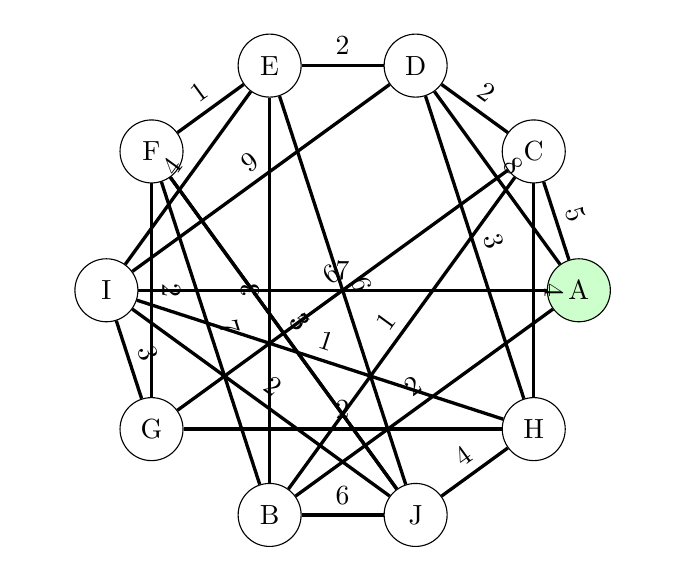
\begin{tikzpicture}
  \filldraw[fill=white!0, draw=none] (-4cm,0) rectangle (4cm, -3cm);
  \node[circle, draw, minimum size=8mm, fill=green!20] (A) at (0.0:3cm) {A};
  \node[circle, draw, minimum size=8mm, fill=white] (C) at (36.0:3cm) {C};
  \node[circle, draw, minimum size=8mm, fill=white] (D) at (72.0:3cm) {D};
  \node[circle, draw, minimum size=8mm, fill=white] (E) at (108.0:3cm) {E};
  \node[circle, draw, minimum size=8mm, fill=white] (F) at (144.0:3cm) {F};
  \node[circle, draw, minimum size=8mm, fill=white] (I) at (180.0:3cm) {I};
  \node[circle, draw, minimum size=8mm, fill=white] (G) at (216.0:3cm) {G};
  \node[circle, draw, minimum size=8mm, fill=white] (B) at (252.0:3cm) {B};
  \node[circle, draw, minimum size=8mm, fill=white] (J) at (288.0:3cm) {J};
  \node[circle, draw, minimum size=8mm, fill=white] (H) at (324.0:3cm) {H};
  \draw[black, line width=1.2pt] (A) -- node[midway, sloped, above] {2} (B);
  \draw[black, line width=1.2pt] (A) -- node[midway, sloped, above] {5} (C);
  \draw[black, line width=1.2pt] (A) -- node[midway, sloped, above] {8} (D);
  \draw[black, line width=1.2pt] (C) -- node[midway, sloped, above] {2} (D);
  \draw[black, line width=1.2pt] (C) -- node[midway, sloped, above] {6} (G);
  \draw[black, line width=1.2pt] (C) -- node[midway, sloped, above] {4} (H);
  \draw[black, line width=1.2pt] (D) -- node[midway, sloped, above] {2} (E);
  \draw[black, line width=1.2pt] (D) -- node[midway, sloped, above] {3} (H);
  \draw[black, line width=1.2pt] (D) -- node[midway, sloped, above] {9} (I);
  \draw[black, line width=1.2pt] (E) -- node[midway, sloped, above] {1} (F);
  \draw[black, line width=1.2pt] (E) -- node[midway, sloped, above] {4} (I);
  \draw[black, line width=1.2pt] (E) -- node[midway, sloped, above] {6} (J);
  \draw[black, line width=1.2pt] (F) -- node[midway, sloped, above] {2} (G);
  \draw[black, line width=1.2pt] (F) -- node[midway, sloped, above] {5} (J);
  \draw[black, line width=1.2pt] (I) -- node[midway, sloped, above] {2} (J);
  \draw[black, line width=1.2pt] (I) -- node[midway, sloped, above] {7} (A);
  \draw[black, line width=1.2pt] (G) -- node[midway, sloped, above] {2} (H);
  \draw[black, line width=1.2pt] (G) -- node[midway, sloped, above] {3} (I);
  \draw[black, line width=1.2pt] (B) -- node[midway, sloped, above] {1} (C);
  \draw[black, line width=1.2pt] (B) -- node[midway, sloped, above] {3} (E);
  \draw[black, line width=1.2pt] (B) -- node[midway, sloped, above] {7} (F);
  \draw[black, line width=1.2pt] (J) -- node[midway, sloped, above] {6} (B);
  \draw[black, line width=1.2pt] (J) -- node[midway, sloped, above] {3} (F);
  \draw[black, line width=1.2pt] (H) -- node[midway, sloped, above] {1} (I);
  \draw[black, line width=1.2pt] (H) -- node[midway, sloped, above] {4} (J);
\end{tikzpicture}
\end{center}
\noindent\rule{\linewidth}{0.3pt}
\begin{center}
\begin{flushleft}\textbf{Open Set}\\[1.75mm]\end{flushleft}
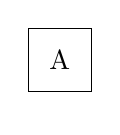
\begin{tikzpicture}
  \filldraw[fill=white!0, draw=none] (0cm,0cm) rectangle (0.8cm, -1cm);
  \filldraw[fill=white] (0cm,-0.8cm) rectangle (0.8cm,0cm);
  \node at (0.4cm,-0.4cm) {A};
\end{tikzpicture}
\end{center}
\noindent\rule{\linewidth}{0.3pt}
\begin{center}
\begin{flushleft}\textbf{Closed Set}\\[1.75mm]\end{flushleft}
\begin{tikzpicture}
  \filldraw[fill=white!0, draw=none] (0cm,0cm) rectangle (0cm, -1cm);
\end{tikzpicture}
\end{center}
\noindent\rule{\linewidth}{0.3pt}
\begin{center}
\begin{flushleft}\textbf{Node Costs}\\[1.75mm]\end{flushleft}
\begin{tikzpicture}
  \filldraw[fill=white!0, draw=none] (0cm,0) rectangle (0.5cm,3.5cm);
  \node[above] at (0.25cm,0cm) {0};
  \node[below] at (0.25cm,0) {A};
  \filldraw[fill=white!0, draw=none] (0.7cm,0) rectangle (1.2cm,3.5cm);
  \node[above] at (0.95cm,0cm) {0};
  \node[below] at (0.95cm,0) {C};
  \filldraw[fill=white!0, draw=none] (1.4cm,0) rectangle (1.9cm,3.5cm);
  \node[above] at (1.65cm,0cm) {0};
  \node[below] at (1.65cm,0) {D};
  \filldraw[fill=white!0, draw=none] (2.0999999999999996cm,0) rectangle (2.5999999999999996cm,3.5cm);
  \node[above] at (2.3499999999999996cm,0cm) {0};
  \node[below] at (2.3499999999999996cm,0) {E};
  \filldraw[fill=white!0, draw=none] (2.8cm,0) rectangle (3.3cm,3.5cm);
  \node[above] at (3.05cm,0cm) {0};
  \node[below] at (3.05cm,0) {F};
  \filldraw[fill=white!0, draw=none] (3.5cm,0) rectangle (4cm,3.5cm);
  \node[above] at (3.75cm,0cm) {0};
  \node[below] at (3.75cm,0) {I};
  \filldraw[fill=white!0, draw=none] (4.199999999999999cm,0) rectangle (4.699999999999999cm,3.5cm);
  \node[above] at (4.449999999999999cm,0cm) {0};
  \node[below] at (4.449999999999999cm,0) {G};
  \filldraw[fill=white!0, draw=none] (4.8999999999999995cm,0) rectangle (5.3999999999999995cm,3.5cm);
  \node[above] at (5.1499999999999995cm,0cm) {0};
  \node[below] at (5.1499999999999995cm,0) {B};
  \filldraw[fill=white!0, draw=none] (5.6cm,0) rectangle (6.1cm,3.5cm);
  \node[above] at (5.85cm,0cm) {0};
  \node[below] at (5.85cm,0) {J};
  \filldraw[fill=white!0, draw=none] (6.3cm,0) rectangle (6.8cm,3.5cm);
  \node[above] at (6.55cm,0cm) {0};
  \node[below] at (6.55cm,0) {H};
\end{tikzpicture}
\end{center}
\newpage
% --- Frame 1 ---
\begin{center}\LARGE\textbf{A* Algorithm}\\[6mm]\end{center}
\begin{center}
\begin{flushleft}\textbf{Log}\\[1.75mm]\end{flushleft}

\begin{tikzpicture}
  \filldraw[fill=white!0, draw=none] (0,0) rectangle (10cm, -0.25cm);
  \node[anchor=north, align=center, text=black] at (5cm,0) {\texttt{Grabbing first node from open set}};
\end{tikzpicture}
\end{center}
\noindent\rule{\linewidth}{0.3pt}
\begin{center}
\begin{flushleft}\textbf{Graph}\\[2mm]\end{flushleft}
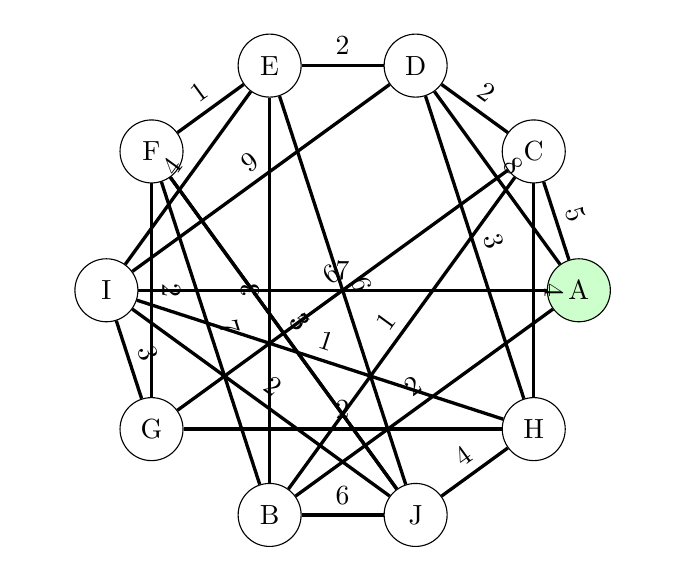
\begin{tikzpicture}
  \filldraw[fill=white!0, draw=none] (-4cm,0) rectangle (4cm, -3cm);
  \node[circle, draw, minimum size=8mm, fill=green!20] (A) at (0.0:3cm) {A};
  \node[circle, draw, minimum size=8mm, fill=white] (C) at (36.0:3cm) {C};
  \node[circle, draw, minimum size=8mm, fill=white] (D) at (72.0:3cm) {D};
  \node[circle, draw, minimum size=8mm, fill=white] (E) at (108.0:3cm) {E};
  \node[circle, draw, minimum size=8mm, fill=white] (F) at (144.0:3cm) {F};
  \node[circle, draw, minimum size=8mm, fill=white] (I) at (180.0:3cm) {I};
  \node[circle, draw, minimum size=8mm, fill=white] (G) at (216.0:3cm) {G};
  \node[circle, draw, minimum size=8mm, fill=white] (B) at (252.0:3cm) {B};
  \node[circle, draw, minimum size=8mm, fill=white] (J) at (288.0:3cm) {J};
  \node[circle, draw, minimum size=8mm, fill=white] (H) at (324.0:3cm) {H};
  \draw[black, line width=1.2pt] (A) -- node[midway, sloped, above] {2} (B);
  \draw[black, line width=1.2pt] (A) -- node[midway, sloped, above] {5} (C);
  \draw[black, line width=1.2pt] (A) -- node[midway, sloped, above] {8} (D);
  \draw[black, line width=1.2pt] (C) -- node[midway, sloped, above] {2} (D);
  \draw[black, line width=1.2pt] (C) -- node[midway, sloped, above] {6} (G);
  \draw[black, line width=1.2pt] (C) -- node[midway, sloped, above] {4} (H);
  \draw[black, line width=1.2pt] (D) -- node[midway, sloped, above] {2} (E);
  \draw[black, line width=1.2pt] (D) -- node[midway, sloped, above] {3} (H);
  \draw[black, line width=1.2pt] (D) -- node[midway, sloped, above] {9} (I);
  \draw[black, line width=1.2pt] (E) -- node[midway, sloped, above] {1} (F);
  \draw[black, line width=1.2pt] (E) -- node[midway, sloped, above] {4} (I);
  \draw[black, line width=1.2pt] (E) -- node[midway, sloped, above] {6} (J);
  \draw[black, line width=1.2pt] (F) -- node[midway, sloped, above] {2} (G);
  \draw[black, line width=1.2pt] (F) -- node[midway, sloped, above] {5} (J);
  \draw[black, line width=1.2pt] (I) -- node[midway, sloped, above] {2} (J);
  \draw[black, line width=1.2pt] (I) -- node[midway, sloped, above] {7} (A);
  \draw[black, line width=1.2pt] (G) -- node[midway, sloped, above] {2} (H);
  \draw[black, line width=1.2pt] (G) -- node[midway, sloped, above] {3} (I);
  \draw[black, line width=1.2pt] (B) -- node[midway, sloped, above] {1} (C);
  \draw[black, line width=1.2pt] (B) -- node[midway, sloped, above] {3} (E);
  \draw[black, line width=1.2pt] (B) -- node[midway, sloped, above] {7} (F);
  \draw[black, line width=1.2pt] (J) -- node[midway, sloped, above] {6} (B);
  \draw[black, line width=1.2pt] (J) -- node[midway, sloped, above] {3} (F);
  \draw[black, line width=1.2pt] (H) -- node[midway, sloped, above] {1} (I);
  \draw[black, line width=1.2pt] (H) -- node[midway, sloped, above] {4} (J);
\end{tikzpicture}
\end{center}
\noindent\rule{\linewidth}{0.3pt}
\begin{center}
\begin{flushleft}\textbf{Open Set}\\[1.75mm]\end{flushleft}
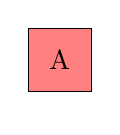
\begin{tikzpicture}
  \filldraw[fill=white!0, draw=none] (0cm,0cm) rectangle (0.8cm, -1cm);
  \filldraw[fill=red!50] (0cm,-0.8cm) rectangle (0.8cm,0cm);
  \node at (0.4cm,-0.4cm) {A};
\end{tikzpicture}
\end{center}
\noindent\rule{\linewidth}{0.3pt}
\begin{center}
\begin{flushleft}\textbf{Closed Set}\\[1.75mm]\end{flushleft}
\begin{tikzpicture}
  \filldraw[fill=white!0, draw=none] (0cm,0cm) rectangle (0cm, -1cm);
\end{tikzpicture}
\end{center}
\noindent\rule{\linewidth}{0.3pt}
\begin{center}
\begin{flushleft}\textbf{Node Costs}\\[1.75mm]\end{flushleft}
\begin{tikzpicture}
  \filldraw[fill=white!0, draw=none] (0cm,0) rectangle (0.5cm,3.5cm);
  \node[above] at (0.25cm,0cm) {0};
  \node[below] at (0.25cm,0) {A};
  \filldraw[fill=white!0, draw=none] (0.7cm,0) rectangle (1.2cm,3.5cm);
  \node[above] at (0.95cm,0cm) {0};
  \node[below] at (0.95cm,0) {C};
  \filldraw[fill=white!0, draw=none] (1.4cm,0) rectangle (1.9cm,3.5cm);
  \node[above] at (1.65cm,0cm) {0};
  \node[below] at (1.65cm,0) {D};
  \filldraw[fill=white!0, draw=none] (2.0999999999999996cm,0) rectangle (2.5999999999999996cm,3.5cm);
  \node[above] at (2.3499999999999996cm,0cm) {0};
  \node[below] at (2.3499999999999996cm,0) {E};
  \filldraw[fill=white!0, draw=none] (2.8cm,0) rectangle (3.3cm,3.5cm);
  \node[above] at (3.05cm,0cm) {0};
  \node[below] at (3.05cm,0) {F};
  \filldraw[fill=white!0, draw=none] (3.5cm,0) rectangle (4cm,3.5cm);
  \node[above] at (3.75cm,0cm) {0};
  \node[below] at (3.75cm,0) {I};
  \filldraw[fill=white!0, draw=none] (4.199999999999999cm,0) rectangle (4.699999999999999cm,3.5cm);
  \node[above] at (4.449999999999999cm,0cm) {0};
  \node[below] at (4.449999999999999cm,0) {G};
  \filldraw[fill=white!0, draw=none] (4.8999999999999995cm,0) rectangle (5.3999999999999995cm,3.5cm);
  \node[above] at (5.1499999999999995cm,0cm) {0};
  \node[below] at (5.1499999999999995cm,0) {B};
  \filldraw[fill=white!0, draw=none] (5.6cm,0) rectangle (6.1cm,3.5cm);
  \node[above] at (5.85cm,0cm) {0};
  \node[below] at (5.85cm,0) {J};
  \filldraw[fill=white!0, draw=none] (6.3cm,0) rectangle (6.8cm,3.5cm);
  \node[above] at (6.55cm,0cm) {0};
  \node[below] at (6.55cm,0) {H};
\end{tikzpicture}
\end{center}
\newpage
% --- Frame 2 ---
\begin{center}\LARGE\textbf{A* Algorithm}\\[6mm]\end{center}
\begin{center}
\begin{flushleft}\textbf{Log}\\[1.75mm]\end{flushleft}

\begin{tikzpicture}
  \filldraw[fill=white!0, draw=none] (0,0) rectangle (10cm, -0.25cm);
  \node[anchor=north, align=center, text=black] at (5cm,0) {\texttt{Visiting node A and adding it to closed set}};
\end{tikzpicture}
\end{center}
\noindent\rule{\linewidth}{0.3pt}
\begin{center}
\begin{flushleft}\textbf{Graph}\\[2mm]\end{flushleft}
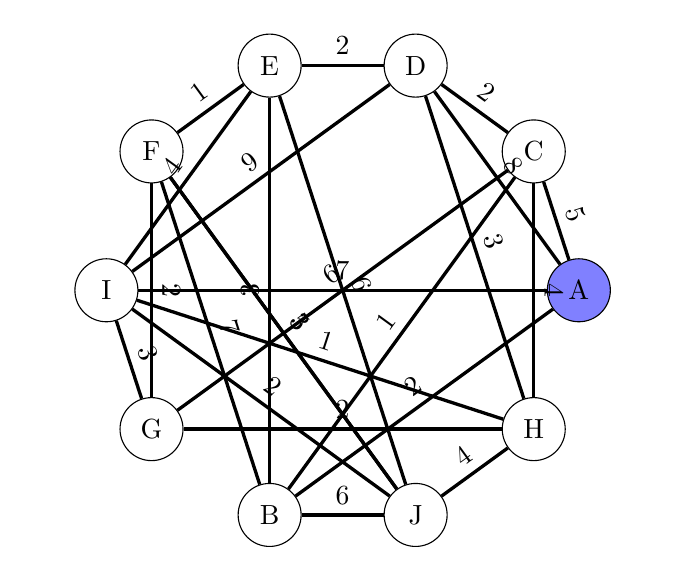
\begin{tikzpicture}
  \filldraw[fill=white!0, draw=none] (-4cm,0) rectangle (4cm, -3cm);
  \node[circle, draw, minimum size=8mm, fill=blue!50] (A) at (0.0:3cm) {A};
  \node[circle, draw, minimum size=8mm, fill=white] (C) at (36.0:3cm) {C};
  \node[circle, draw, minimum size=8mm, fill=white] (D) at (72.0:3cm) {D};
  \node[circle, draw, minimum size=8mm, fill=white] (E) at (108.0:3cm) {E};
  \node[circle, draw, minimum size=8mm, fill=white] (F) at (144.0:3cm) {F};
  \node[circle, draw, minimum size=8mm, fill=white] (I) at (180.0:3cm) {I};
  \node[circle, draw, minimum size=8mm, fill=white] (G) at (216.0:3cm) {G};
  \node[circle, draw, minimum size=8mm, fill=white] (B) at (252.0:3cm) {B};
  \node[circle, draw, minimum size=8mm, fill=white] (J) at (288.0:3cm) {J};
  \node[circle, draw, minimum size=8mm, fill=white] (H) at (324.0:3cm) {H};
  \draw[black, line width=1.2pt] (A) -- node[midway, sloped, above] {2} (B);
  \draw[black, line width=1.2pt] (A) -- node[midway, sloped, above] {5} (C);
  \draw[black, line width=1.2pt] (A) -- node[midway, sloped, above] {8} (D);
  \draw[black, line width=1.2pt] (C) -- node[midway, sloped, above] {2} (D);
  \draw[black, line width=1.2pt] (C) -- node[midway, sloped, above] {6} (G);
  \draw[black, line width=1.2pt] (C) -- node[midway, sloped, above] {4} (H);
  \draw[black, line width=1.2pt] (D) -- node[midway, sloped, above] {2} (E);
  \draw[black, line width=1.2pt] (D) -- node[midway, sloped, above] {3} (H);
  \draw[black, line width=1.2pt] (D) -- node[midway, sloped, above] {9} (I);
  \draw[black, line width=1.2pt] (E) -- node[midway, sloped, above] {1} (F);
  \draw[black, line width=1.2pt] (E) -- node[midway, sloped, above] {4} (I);
  \draw[black, line width=1.2pt] (E) -- node[midway, sloped, above] {6} (J);
  \draw[black, line width=1.2pt] (F) -- node[midway, sloped, above] {2} (G);
  \draw[black, line width=1.2pt] (F) -- node[midway, sloped, above] {5} (J);
  \draw[black, line width=1.2pt] (I) -- node[midway, sloped, above] {2} (J);
  \draw[black, line width=1.2pt] (I) -- node[midway, sloped, above] {7} (A);
  \draw[black, line width=1.2pt] (G) -- node[midway, sloped, above] {2} (H);
  \draw[black, line width=1.2pt] (G) -- node[midway, sloped, above] {3} (I);
  \draw[black, line width=1.2pt] (B) -- node[midway, sloped, above] {1} (C);
  \draw[black, line width=1.2pt] (B) -- node[midway, sloped, above] {3} (E);
  \draw[black, line width=1.2pt] (B) -- node[midway, sloped, above] {7} (F);
  \draw[black, line width=1.2pt] (J) -- node[midway, sloped, above] {6} (B);
  \draw[black, line width=1.2pt] (J) -- node[midway, sloped, above] {3} (F);
  \draw[black, line width=1.2pt] (H) -- node[midway, sloped, above] {1} (I);
  \draw[black, line width=1.2pt] (H) -- node[midway, sloped, above] {4} (J);
\end{tikzpicture}
\end{center}
\noindent\rule{\linewidth}{0.3pt}
\begin{center}
\begin{flushleft}\textbf{Open Set}\\[1.75mm]\end{flushleft}
\begin{tikzpicture}
  \filldraw[fill=white!0, draw=none] (0cm,0cm) rectangle (0cm, -1cm);
\end{tikzpicture}
\end{center}
\noindent\rule{\linewidth}{0.3pt}
\begin{center}
\begin{flushleft}\textbf{Closed Set}\\[1.75mm]\end{flushleft}
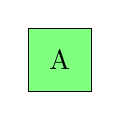
\begin{tikzpicture}
  \filldraw[fill=white!0, draw=none] (0cm,0cm) rectangle (0.8cm, -1cm);
  \filldraw[fill=green!50] (0cm,-0.8cm) rectangle (0.8cm,0cm);
  \node at (0.4cm,-0.4cm) {A};
\end{tikzpicture}
\end{center}
\noindent\rule{\linewidth}{0.3pt}
\begin{center}
\begin{flushleft}\textbf{Node Costs}\\[1.75mm]\end{flushleft}
\begin{tikzpicture}
  \filldraw[fill=white!0, draw=none] (0cm,0) rectangle (0.5cm,3.5cm);
  \node[above] at (0.25cm,0cm) {0};
  \node[below] at (0.25cm,0) {A};
  \filldraw[fill=white!0, draw=none] (0.7cm,0) rectangle (1.2cm,3.5cm);
  \node[above] at (0.95cm,0cm) {0};
  \node[below] at (0.95cm,0) {C};
  \filldraw[fill=white!0, draw=none] (1.4cm,0) rectangle (1.9cm,3.5cm);
  \node[above] at (1.65cm,0cm) {0};
  \node[below] at (1.65cm,0) {D};
  \filldraw[fill=white!0, draw=none] (2.0999999999999996cm,0) rectangle (2.5999999999999996cm,3.5cm);
  \node[above] at (2.3499999999999996cm,0cm) {0};
  \node[below] at (2.3499999999999996cm,0) {E};
  \filldraw[fill=white!0, draw=none] (2.8cm,0) rectangle (3.3cm,3.5cm);
  \node[above] at (3.05cm,0cm) {0};
  \node[below] at (3.05cm,0) {F};
  \filldraw[fill=white!0, draw=none] (3.5cm,0) rectangle (4cm,3.5cm);
  \node[above] at (3.75cm,0cm) {0};
  \node[below] at (3.75cm,0) {I};
  \filldraw[fill=white!0, draw=none] (4.199999999999999cm,0) rectangle (4.699999999999999cm,3.5cm);
  \node[above] at (4.449999999999999cm,0cm) {0};
  \node[below] at (4.449999999999999cm,0) {G};
  \filldraw[fill=white!0, draw=none] (4.8999999999999995cm,0) rectangle (5.3999999999999995cm,3.5cm);
  \node[above] at (5.1499999999999995cm,0cm) {0};
  \node[below] at (5.1499999999999995cm,0) {B};
  \filldraw[fill=white!0, draw=none] (5.6cm,0) rectangle (6.1cm,3.5cm);
  \node[above] at (5.85cm,0cm) {0};
  \node[below] at (5.85cm,0) {J};
  \filldraw[fill=white!0, draw=none] (6.3cm,0) rectangle (6.8cm,3.5cm);
  \node[above] at (6.55cm,0cm) {0};
  \node[below] at (6.55cm,0) {H};
\end{tikzpicture}
\end{center}
\newpage
% --- Frame 3 ---
\begin{center}\LARGE\textbf{A* Algorithm}\\[6mm]\end{center}
\begin{center}
\begin{flushleft}\textbf{Log}\\[1.75mm]\end{flushleft}

\begin{tikzpicture}
  \filldraw[fill=white!0, draw=none] (0,0) rectangle (10cm, -0.25cm);
  \node[anchor=north, align=center, text=black] at (5cm,0) {\texttt{Checking neighbor B}};
\end{tikzpicture}
\end{center}
\noindent\rule{\linewidth}{0.3pt}
\begin{center}
\begin{flushleft}\textbf{Graph}\\[2mm]\end{flushleft}
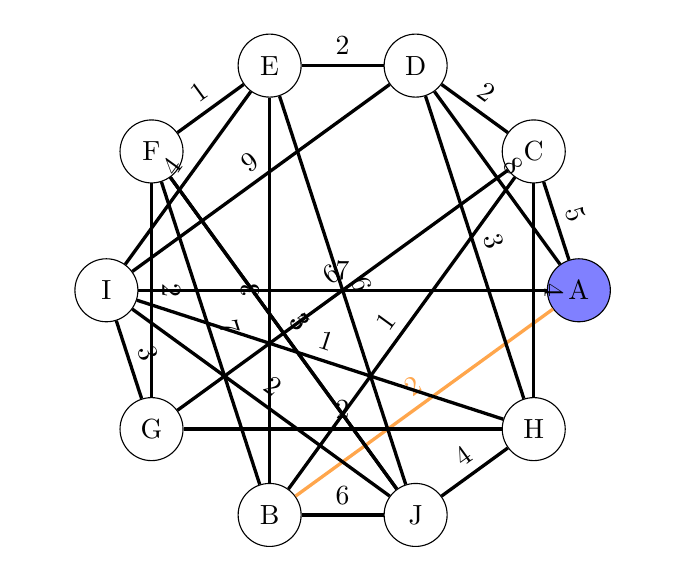
\begin{tikzpicture}
  \filldraw[fill=white!0, draw=none] (-4cm,0) rectangle (4cm, -3cm);
  \node[circle, draw, minimum size=8mm, fill=blue!50] (A) at (0.0:3cm) {A};
  \node[circle, draw, minimum size=8mm, fill=white] (C) at (36.0:3cm) {C};
  \node[circle, draw, minimum size=8mm, fill=white] (D) at (72.0:3cm) {D};
  \node[circle, draw, minimum size=8mm, fill=white] (E) at (108.0:3cm) {E};
  \node[circle, draw, minimum size=8mm, fill=white] (F) at (144.0:3cm) {F};
  \node[circle, draw, minimum size=8mm, fill=white] (I) at (180.0:3cm) {I};
  \node[circle, draw, minimum size=8mm, fill=white] (G) at (216.0:3cm) {G};
  \node[circle, draw, minimum size=8mm, fill=white] (B) at (252.0:3cm) {B};
  \node[circle, draw, minimum size=8mm, fill=white] (J) at (288.0:3cm) {J};
  \node[circle, draw, minimum size=8mm, fill=white] (H) at (324.0:3cm) {H};
  \draw[orange!70, line width=1.2pt] (A) -- node[midway, sloped, above] {2} (B);
  \draw[black, line width=1.2pt] (A) -- node[midway, sloped, above] {5} (C);
  \draw[black, line width=1.2pt] (A) -- node[midway, sloped, above] {8} (D);
  \draw[black, line width=1.2pt] (C) -- node[midway, sloped, above] {2} (D);
  \draw[black, line width=1.2pt] (C) -- node[midway, sloped, above] {6} (G);
  \draw[black, line width=1.2pt] (C) -- node[midway, sloped, above] {4} (H);
  \draw[black, line width=1.2pt] (D) -- node[midway, sloped, above] {2} (E);
  \draw[black, line width=1.2pt] (D) -- node[midway, sloped, above] {3} (H);
  \draw[black, line width=1.2pt] (D) -- node[midway, sloped, above] {9} (I);
  \draw[black, line width=1.2pt] (E) -- node[midway, sloped, above] {1} (F);
  \draw[black, line width=1.2pt] (E) -- node[midway, sloped, above] {4} (I);
  \draw[black, line width=1.2pt] (E) -- node[midway, sloped, above] {6} (J);
  \draw[black, line width=1.2pt] (F) -- node[midway, sloped, above] {2} (G);
  \draw[black, line width=1.2pt] (F) -- node[midway, sloped, above] {5} (J);
  \draw[black, line width=1.2pt] (I) -- node[midway, sloped, above] {2} (J);
  \draw[black, line width=1.2pt] (I) -- node[midway, sloped, above] {7} (A);
  \draw[black, line width=1.2pt] (G) -- node[midway, sloped, above] {2} (H);
  \draw[black, line width=1.2pt] (G) -- node[midway, sloped, above] {3} (I);
  \draw[black, line width=1.2pt] (B) -- node[midway, sloped, above] {1} (C);
  \draw[black, line width=1.2pt] (B) -- node[midway, sloped, above] {3} (E);
  \draw[black, line width=1.2pt] (B) -- node[midway, sloped, above] {7} (F);
  \draw[black, line width=1.2pt] (J) -- node[midway, sloped, above] {6} (B);
  \draw[black, line width=1.2pt] (J) -- node[midway, sloped, above] {3} (F);
  \draw[black, line width=1.2pt] (H) -- node[midway, sloped, above] {1} (I);
  \draw[black, line width=1.2pt] (H) -- node[midway, sloped, above] {4} (J);
\end{tikzpicture}
\end{center}
\noindent\rule{\linewidth}{0.3pt}
\begin{center}
\begin{flushleft}\textbf{Open Set}\\[1.75mm]\end{flushleft}
\begin{tikzpicture}
  \filldraw[fill=white!0, draw=none] (0cm,0cm) rectangle (0cm, -1cm);
\end{tikzpicture}
\end{center}
\noindent\rule{\linewidth}{0.3pt}
\begin{center}
\begin{flushleft}\textbf{Closed Set}\\[1.75mm]\end{flushleft}
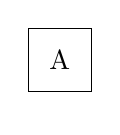
\begin{tikzpicture}
  \filldraw[fill=white!0, draw=none] (0cm,0cm) rectangle (0.8cm, -1cm);
  \filldraw[fill=white] (0cm,-0.8cm) rectangle (0.8cm,0cm);
  \node at (0.4cm,-0.4cm) {A};
\end{tikzpicture}
\end{center}
\noindent\rule{\linewidth}{0.3pt}
\begin{center}
\begin{flushleft}\textbf{Node Costs}\\[1.75mm]\end{flushleft}
\begin{tikzpicture}
  \filldraw[fill=white!0, draw=none] (0cm,0) rectangle (0.5cm,3.5cm);
  \node[above] at (0.25cm,0cm) {0};
  \node[below] at (0.25cm,0) {A};
  \filldraw[fill=white!0, draw=none] (0.7cm,0) rectangle (1.2cm,3.5cm);
  \node[above] at (0.95cm,0cm) {0};
  \node[below] at (0.95cm,0) {C};
  \filldraw[fill=white!0, draw=none] (1.4cm,0) rectangle (1.9cm,3.5cm);
  \node[above] at (1.65cm,0cm) {0};
  \node[below] at (1.65cm,0) {D};
  \filldraw[fill=white!0, draw=none] (2.0999999999999996cm,0) rectangle (2.5999999999999996cm,3.5cm);
  \node[above] at (2.3499999999999996cm,0cm) {0};
  \node[below] at (2.3499999999999996cm,0) {E};
  \filldraw[fill=white!0, draw=none] (2.8cm,0) rectangle (3.3cm,3.5cm);
  \node[above] at (3.05cm,0cm) {0};
  \node[below] at (3.05cm,0) {F};
  \filldraw[fill=white!0, draw=none] (3.5cm,0) rectangle (4cm,3.5cm);
  \node[above] at (3.75cm,0cm) {0};
  \node[below] at (3.75cm,0) {I};
  \filldraw[fill=white!0, draw=none] (4.199999999999999cm,0) rectangle (4.699999999999999cm,3.5cm);
  \node[above] at (4.449999999999999cm,0cm) {0};
  \node[below] at (4.449999999999999cm,0) {G};
  \filldraw[fill=white!0, draw=none] (4.8999999999999995cm,0) rectangle (5.3999999999999995cm,3.5cm);
  \node[above] at (5.1499999999999995cm,0cm) {0};
  \node[below] at (5.1499999999999995cm,0) {B};
  \filldraw[fill=white!0, draw=none] (5.6cm,0) rectangle (6.1cm,3.5cm);
  \node[above] at (5.85cm,0cm) {0};
  \node[below] at (5.85cm,0) {J};
  \filldraw[fill=white!0, draw=none] (6.3cm,0) rectangle (6.8cm,3.5cm);
  \node[above] at (6.55cm,0cm) {0};
  \node[below] at (6.55cm,0) {H};
\end{tikzpicture}
\end{center}
\newpage
% --- Frame 4 ---
\begin{center}\LARGE\textbf{A* Algorithm}\\[6mm]\end{center}
\begin{center}
\begin{flushleft}\textbf{Log}\\[1.75mm]\end{flushleft}

\begin{tikzpicture}
  \filldraw[fill=white!0, draw=none] (0,0) rectangle (10cm, -0.25cm);
  \node[anchor=north, align=center, text=black] at (5cm,0) {\texttt{Adding neighbor B to open set}};
\end{tikzpicture}
\end{center}
\noindent\rule{\linewidth}{0.3pt}
\begin{center}
\begin{flushleft}\textbf{Graph}\\[2mm]\end{flushleft}
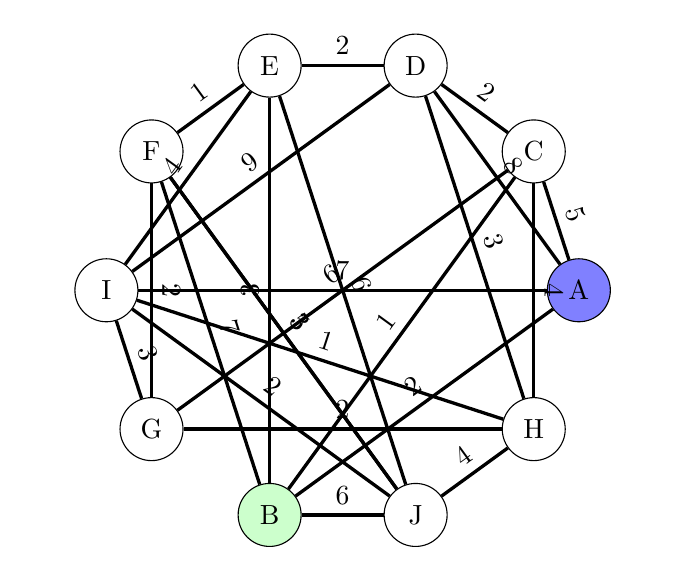
\begin{tikzpicture}
  \filldraw[fill=white!0, draw=none] (-4cm,0) rectangle (4cm, -3cm);
  \node[circle, draw, minimum size=8mm, fill=blue!50] (A) at (0.0:3cm) {A};
  \node[circle, draw, minimum size=8mm, fill=white] (C) at (36.0:3cm) {C};
  \node[circle, draw, minimum size=8mm, fill=white] (D) at (72.0:3cm) {D};
  \node[circle, draw, minimum size=8mm, fill=white] (E) at (108.0:3cm) {E};
  \node[circle, draw, minimum size=8mm, fill=white] (F) at (144.0:3cm) {F};
  \node[circle, draw, minimum size=8mm, fill=white] (I) at (180.0:3cm) {I};
  \node[circle, draw, minimum size=8mm, fill=white] (G) at (216.0:3cm) {G};
  \node[circle, draw, minimum size=8mm, fill=green!20] (B) at (252.0:3cm) {B};
  \node[circle, draw, minimum size=8mm, fill=white] (J) at (288.0:3cm) {J};
  \node[circle, draw, minimum size=8mm, fill=white] (H) at (324.0:3cm) {H};
  \draw[black, line width=1.2pt] (A) -- node[midway, sloped, above] {2} (B);
  \draw[black, line width=1.2pt] (A) -- node[midway, sloped, above] {5} (C);
  \draw[black, line width=1.2pt] (A) -- node[midway, sloped, above] {8} (D);
  \draw[black, line width=1.2pt] (C) -- node[midway, sloped, above] {2} (D);
  \draw[black, line width=1.2pt] (C) -- node[midway, sloped, above] {6} (G);
  \draw[black, line width=1.2pt] (C) -- node[midway, sloped, above] {4} (H);
  \draw[black, line width=1.2pt] (D) -- node[midway, sloped, above] {2} (E);
  \draw[black, line width=1.2pt] (D) -- node[midway, sloped, above] {3} (H);
  \draw[black, line width=1.2pt] (D) -- node[midway, sloped, above] {9} (I);
  \draw[black, line width=1.2pt] (E) -- node[midway, sloped, above] {1} (F);
  \draw[black, line width=1.2pt] (E) -- node[midway, sloped, above] {4} (I);
  \draw[black, line width=1.2pt] (E) -- node[midway, sloped, above] {6} (J);
  \draw[black, line width=1.2pt] (F) -- node[midway, sloped, above] {2} (G);
  \draw[black, line width=1.2pt] (F) -- node[midway, sloped, above] {5} (J);
  \draw[black, line width=1.2pt] (I) -- node[midway, sloped, above] {2} (J);
  \draw[black, line width=1.2pt] (I) -- node[midway, sloped, above] {7} (A);
  \draw[black, line width=1.2pt] (G) -- node[midway, sloped, above] {2} (H);
  \draw[black, line width=1.2pt] (G) -- node[midway, sloped, above] {3} (I);
  \draw[black, line width=1.2pt] (B) -- node[midway, sloped, above] {1} (C);
  \draw[black, line width=1.2pt] (B) -- node[midway, sloped, above] {3} (E);
  \draw[black, line width=1.2pt] (B) -- node[midway, sloped, above] {7} (F);
  \draw[black, line width=1.2pt] (J) -- node[midway, sloped, above] {6} (B);
  \draw[black, line width=1.2pt] (J) -- node[midway, sloped, above] {3} (F);
  \draw[black, line width=1.2pt] (H) -- node[midway, sloped, above] {1} (I);
  \draw[black, line width=1.2pt] (H) -- node[midway, sloped, above] {4} (J);
\end{tikzpicture}
\end{center}
\noindent\rule{\linewidth}{0.3pt}
\begin{center}
\begin{flushleft}\textbf{Open Set}\\[1.75mm]\end{flushleft}
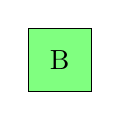
\begin{tikzpicture}
  \filldraw[fill=white!0, draw=none] (0cm,0cm) rectangle (0.8cm, -1cm);
  \filldraw[fill=green!50] (0cm,-0.8cm) rectangle (0.8cm,0cm);
  \node at (0.4cm,-0.4cm) {B};
\end{tikzpicture}
\end{center}
\noindent\rule{\linewidth}{0.3pt}
\begin{center}
\begin{flushleft}\textbf{Closed Set}\\[1.75mm]\end{flushleft}
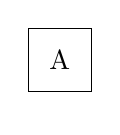
\begin{tikzpicture}
  \filldraw[fill=white!0, draw=none] (0cm,0cm) rectangle (0.8cm, -1cm);
  \filldraw[fill=white] (0cm,-0.8cm) rectangle (0.8cm,0cm);
  \node at (0.4cm,-0.4cm) {A};
\end{tikzpicture}
\end{center}
\noindent\rule{\linewidth}{0.3pt}
\begin{center}
\begin{flushleft}\textbf{Node Costs}\\[1.75mm]\end{flushleft}
\begin{tikzpicture}
  \filldraw[fill=white!0, draw=none] (0cm,0) rectangle (0.5cm,3.5cm);
  \node[above] at (0.25cm,0cm) {0};
  \node[below] at (0.25cm,0) {A};
  \filldraw[fill=white!0, draw=none] (0.7cm,0) rectangle (1.2cm,3.5cm);
  \node[above] at (0.95cm,0cm) {0};
  \node[below] at (0.95cm,0) {C};
  \filldraw[fill=white!0, draw=none] (1.4cm,0) rectangle (1.9cm,3.5cm);
  \node[above] at (1.65cm,0cm) {0};
  \node[below] at (1.65cm,0) {D};
  \filldraw[fill=white!0, draw=none] (2.0999999999999996cm,0) rectangle (2.5999999999999996cm,3.5cm);
  \node[above] at (2.3499999999999996cm,0cm) {0};
  \node[below] at (2.3499999999999996cm,0) {E};
  \filldraw[fill=white!0, draw=none] (2.8cm,0) rectangle (3.3cm,3.5cm);
  \node[above] at (3.05cm,0cm) {0};
  \node[below] at (3.05cm,0) {F};
  \filldraw[fill=white!0, draw=none] (3.5cm,0) rectangle (4cm,3.5cm);
  \node[above] at (3.75cm,0cm) {0};
  \node[below] at (3.75cm,0) {I};
  \filldraw[fill=white!0, draw=none] (4.199999999999999cm,0) rectangle (4.699999999999999cm,3.5cm);
  \node[above] at (4.449999999999999cm,0cm) {0};
  \node[below] at (4.449999999999999cm,0) {G};
  \filldraw[fill=white!0, draw=none] (4.8999999999999995cm,0) rectangle (5.3999999999999995cm,3.5cm);
  \node[above] at (5.1499999999999995cm,0cm) {0};
  \node[below] at (5.1499999999999995cm,0) {B};
  \filldraw[fill=white!0, draw=none] (5.6cm,0) rectangle (6.1cm,3.5cm);
  \node[above] at (5.85cm,0cm) {0};
  \node[below] at (5.85cm,0) {J};
  \filldraw[fill=white!0, draw=none] (6.3cm,0) rectangle (6.8cm,3.5cm);
  \node[above] at (6.55cm,0cm) {0};
  \node[below] at (6.55cm,0) {H};
\end{tikzpicture}
\end{center}
\newpage
% --- Frame 5 ---
\begin{center}\LARGE\textbf{A* Algorithm}\\[6mm]\end{center}
\begin{center}
\begin{flushleft}\textbf{Log}\\[1.75mm]\end{flushleft}

\begin{tikzpicture}
  \filldraw[fill=white!0, draw=none] (0,0) rectangle (10cm, -0.25cm);
  \node[anchor=north, align=center, text=black] at (5cm,0) {\texttt{Updating cost for neighbor B (cost: 2)}};
\end{tikzpicture}
\end{center}
\noindent\rule{\linewidth}{0.3pt}
\begin{center}
\begin{flushleft}\textbf{Graph}\\[2mm]\end{flushleft}
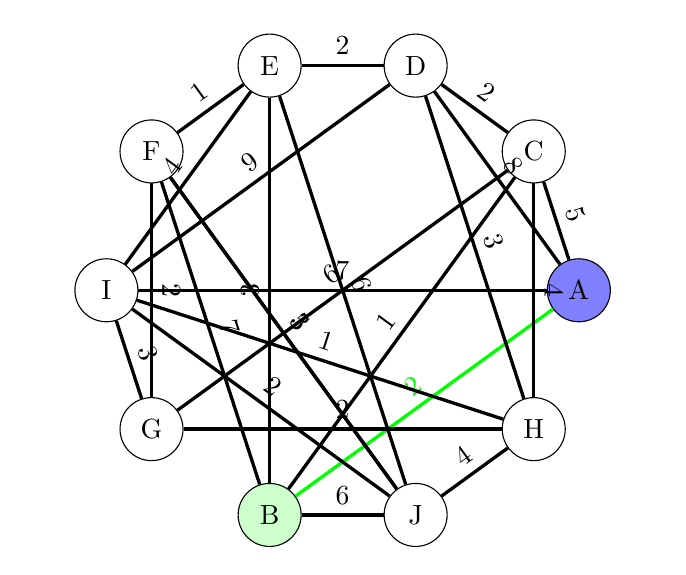
\begin{tikzpicture}
  \filldraw[fill=white!0, draw=none] (-4cm,0) rectangle (4cm, -3cm);
  \node[circle, draw, minimum size=8mm, fill=blue!50] (A) at (0.0:3cm) {A};
  \node[circle, draw, minimum size=8mm, fill=white] (C) at (36.0:3cm) {C};
  \node[circle, draw, minimum size=8mm, fill=white] (D) at (72.0:3cm) {D};
  \node[circle, draw, minimum size=8mm, fill=white] (E) at (108.0:3cm) {E};
  \node[circle, draw, minimum size=8mm, fill=white] (F) at (144.0:3cm) {F};
  \node[circle, draw, minimum size=8mm, fill=white] (I) at (180.0:3cm) {I};
  \node[circle, draw, minimum size=8mm, fill=white] (G) at (216.0:3cm) {G};
  \node[circle, draw, minimum size=8mm, fill=green!20] (B) at (252.0:3cm) {B};
  \node[circle, draw, minimum size=8mm, fill=white] (J) at (288.0:3cm) {J};
  \node[circle, draw, minimum size=8mm, fill=white] (H) at (324.0:3cm) {H};
  \draw[green!100, line width=1.2pt] (A) -- node[midway, sloped, above] {2} (B);
  \draw[black, line width=1.2pt] (A) -- node[midway, sloped, above] {5} (C);
  \draw[black, line width=1.2pt] (A) -- node[midway, sloped, above] {8} (D);
  \draw[black, line width=1.2pt] (C) -- node[midway, sloped, above] {2} (D);
  \draw[black, line width=1.2pt] (C) -- node[midway, sloped, above] {6} (G);
  \draw[black, line width=1.2pt] (C) -- node[midway, sloped, above] {4} (H);
  \draw[black, line width=1.2pt] (D) -- node[midway, sloped, above] {2} (E);
  \draw[black, line width=1.2pt] (D) -- node[midway, sloped, above] {3} (H);
  \draw[black, line width=1.2pt] (D) -- node[midway, sloped, above] {9} (I);
  \draw[black, line width=1.2pt] (E) -- node[midway, sloped, above] {1} (F);
  \draw[black, line width=1.2pt] (E) -- node[midway, sloped, above] {4} (I);
  \draw[black, line width=1.2pt] (E) -- node[midway, sloped, above] {6} (J);
  \draw[black, line width=1.2pt] (F) -- node[midway, sloped, above] {2} (G);
  \draw[black, line width=1.2pt] (F) -- node[midway, sloped, above] {5} (J);
  \draw[black, line width=1.2pt] (I) -- node[midway, sloped, above] {2} (J);
  \draw[black, line width=1.2pt] (I) -- node[midway, sloped, above] {7} (A);
  \draw[black, line width=1.2pt] (G) -- node[midway, sloped, above] {2} (H);
  \draw[black, line width=1.2pt] (G) -- node[midway, sloped, above] {3} (I);
  \draw[black, line width=1.2pt] (B) -- node[midway, sloped, above] {1} (C);
  \draw[black, line width=1.2pt] (B) -- node[midway, sloped, above] {3} (E);
  \draw[black, line width=1.2pt] (B) -- node[midway, sloped, above] {7} (F);
  \draw[black, line width=1.2pt] (J) -- node[midway, sloped, above] {6} (B);
  \draw[black, line width=1.2pt] (J) -- node[midway, sloped, above] {3} (F);
  \draw[black, line width=1.2pt] (H) -- node[midway, sloped, above] {1} (I);
  \draw[black, line width=1.2pt] (H) -- node[midway, sloped, above] {4} (J);
\end{tikzpicture}
\end{center}
\noindent\rule{\linewidth}{0.3pt}
\begin{center}
\begin{flushleft}\textbf{Open Set}\\[1.75mm]\end{flushleft}
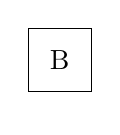
\begin{tikzpicture}
  \filldraw[fill=white!0, draw=none] (0cm,0cm) rectangle (0.8cm, -1cm);
  \filldraw[fill=white] (0cm,-0.8cm) rectangle (0.8cm,0cm);
  \node at (0.4cm,-0.4cm) {B};
\end{tikzpicture}
\end{center}
\noindent\rule{\linewidth}{0.3pt}
\begin{center}
\begin{flushleft}\textbf{Closed Set}\\[1.75mm]\end{flushleft}
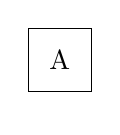
\begin{tikzpicture}
  \filldraw[fill=white!0, draw=none] (0cm,0cm) rectangle (0.8cm, -1cm);
  \filldraw[fill=white] (0cm,-0.8cm) rectangle (0.8cm,0cm);
  \node at (0.4cm,-0.4cm) {A};
\end{tikzpicture}
\end{center}
\noindent\rule{\linewidth}{0.3pt}
\begin{center}
\begin{flushleft}\textbf{Node Costs}\\[1.75mm]\end{flushleft}
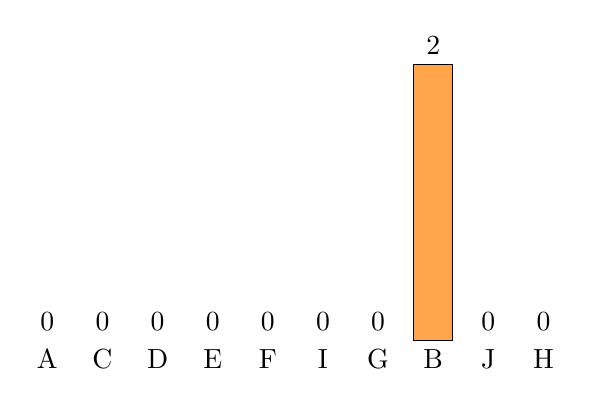
\begin{tikzpicture}
  \filldraw[fill=white!0, draw=none] (0cm,0) rectangle (0.5cm,3.5cm);
  \node[above] at (0.25cm,0cm) {0};
  \node[below] at (0.25cm,0) {A};
  \filldraw[fill=white!0, draw=none] (0.7cm,0) rectangle (1.2cm,3.5cm);
  \node[above] at (0.95cm,0cm) {0};
  \node[below] at (0.95cm,0) {C};
  \filldraw[fill=white!0, draw=none] (1.4cm,0) rectangle (1.9cm,3.5cm);
  \node[above] at (1.65cm,0cm) {0};
  \node[below] at (1.65cm,0) {D};
  \filldraw[fill=white!0, draw=none] (2.0999999999999996cm,0) rectangle (2.5999999999999996cm,3.5cm);
  \node[above] at (2.3499999999999996cm,0cm) {0};
  \node[below] at (2.3499999999999996cm,0) {E};
  \filldraw[fill=white!0, draw=none] (2.8cm,0) rectangle (3.3cm,3.5cm);
  \node[above] at (3.05cm,0cm) {0};
  \node[below] at (3.05cm,0) {F};
  \filldraw[fill=white!0, draw=none] (3.5cm,0) rectangle (4cm,3.5cm);
  \node[above] at (3.75cm,0cm) {0};
  \node[below] at (3.75cm,0) {I};
  \filldraw[fill=white!0, draw=none] (4.199999999999999cm,0) rectangle (4.699999999999999cm,3.5cm);
  \node[above] at (4.449999999999999cm,0cm) {0};
  \node[below] at (4.449999999999999cm,0) {G};
  \filldraw[fill=white!0, draw=none] (4.8999999999999995cm,0) rectangle (5.3999999999999995cm,3.5cm);
  \filldraw[fill=orange!70] (4.8999999999999995cm,0cm) rectangle (5.3999999999999995cm,3.5cm);
  \node[above] at (5.1499999999999995cm,3.5cm) {2};
  \node[below] at (5.1499999999999995cm,0) {B};
  \filldraw[fill=white!0, draw=none] (5.6cm,0) rectangle (6.1cm,3.5cm);
  \node[above] at (5.85cm,0cm) {0};
  \node[below] at (5.85cm,0) {J};
  \filldraw[fill=white!0, draw=none] (6.3cm,0) rectangle (6.8cm,3.5cm);
  \node[above] at (6.55cm,0cm) {0};
  \node[below] at (6.55cm,0) {H};
\end{tikzpicture}
\end{center}
\newpage
% --- Frame 6 ---
\begin{center}\LARGE\textbf{A* Algorithm}\\[6mm]\end{center}
\begin{center}
\begin{flushleft}\textbf{Log}\\[1.75mm]\end{flushleft}

\begin{tikzpicture}
  \filldraw[fill=white!0, draw=none] (0,0) rectangle (10cm, -0.25cm);
  \node[anchor=north, align=center, text=black] at (5cm,0) {\texttt{Checking neighbor C}};
\end{tikzpicture}
\end{center}
\noindent\rule{\linewidth}{0.3pt}
\begin{center}
\begin{flushleft}\textbf{Graph}\\[2mm]\end{flushleft}
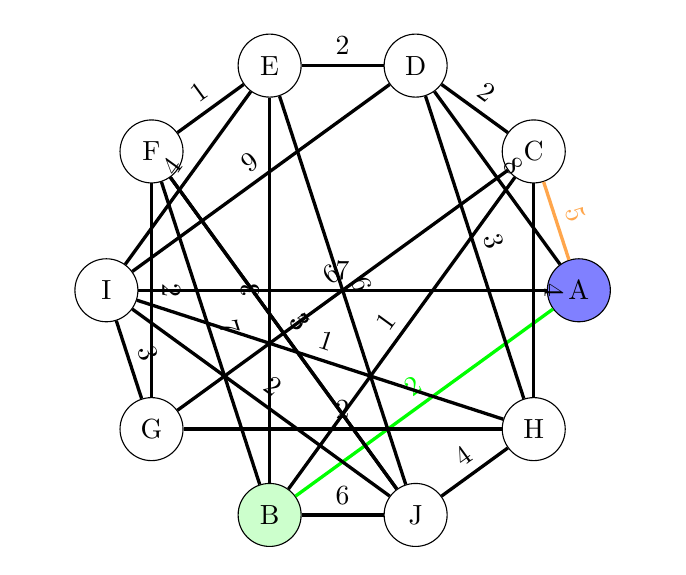
\begin{tikzpicture}
  \filldraw[fill=white!0, draw=none] (-4cm,0) rectangle (4cm, -3cm);
  \node[circle, draw, minimum size=8mm, fill=blue!50] (A) at (0.0:3cm) {A};
  \node[circle, draw, minimum size=8mm, fill=white] (C) at (36.0:3cm) {C};
  \node[circle, draw, minimum size=8mm, fill=white] (D) at (72.0:3cm) {D};
  \node[circle, draw, minimum size=8mm, fill=white] (E) at (108.0:3cm) {E};
  \node[circle, draw, minimum size=8mm, fill=white] (F) at (144.0:3cm) {F};
  \node[circle, draw, minimum size=8mm, fill=white] (I) at (180.0:3cm) {I};
  \node[circle, draw, minimum size=8mm, fill=white] (G) at (216.0:3cm) {G};
  \node[circle, draw, minimum size=8mm, fill=green!20] (B) at (252.0:3cm) {B};
  \node[circle, draw, minimum size=8mm, fill=white] (J) at (288.0:3cm) {J};
  \node[circle, draw, minimum size=8mm, fill=white] (H) at (324.0:3cm) {H};
  \draw[green!100, line width=1.2pt] (A) -- node[midway, sloped, above] {2} (B);
  \draw[orange!70, line width=1.2pt] (A) -- node[midway, sloped, above] {5} (C);
  \draw[black, line width=1.2pt] (A) -- node[midway, sloped, above] {8} (D);
  \draw[black, line width=1.2pt] (C) -- node[midway, sloped, above] {2} (D);
  \draw[black, line width=1.2pt] (C) -- node[midway, sloped, above] {6} (G);
  \draw[black, line width=1.2pt] (C) -- node[midway, sloped, above] {4} (H);
  \draw[black, line width=1.2pt] (D) -- node[midway, sloped, above] {2} (E);
  \draw[black, line width=1.2pt] (D) -- node[midway, sloped, above] {3} (H);
  \draw[black, line width=1.2pt] (D) -- node[midway, sloped, above] {9} (I);
  \draw[black, line width=1.2pt] (E) -- node[midway, sloped, above] {1} (F);
  \draw[black, line width=1.2pt] (E) -- node[midway, sloped, above] {4} (I);
  \draw[black, line width=1.2pt] (E) -- node[midway, sloped, above] {6} (J);
  \draw[black, line width=1.2pt] (F) -- node[midway, sloped, above] {2} (G);
  \draw[black, line width=1.2pt] (F) -- node[midway, sloped, above] {5} (J);
  \draw[black, line width=1.2pt] (I) -- node[midway, sloped, above] {2} (J);
  \draw[black, line width=1.2pt] (I) -- node[midway, sloped, above] {7} (A);
  \draw[black, line width=1.2pt] (G) -- node[midway, sloped, above] {2} (H);
  \draw[black, line width=1.2pt] (G) -- node[midway, sloped, above] {3} (I);
  \draw[black, line width=1.2pt] (B) -- node[midway, sloped, above] {1} (C);
  \draw[black, line width=1.2pt] (B) -- node[midway, sloped, above] {3} (E);
  \draw[black, line width=1.2pt] (B) -- node[midway, sloped, above] {7} (F);
  \draw[black, line width=1.2pt] (J) -- node[midway, sloped, above] {6} (B);
  \draw[black, line width=1.2pt] (J) -- node[midway, sloped, above] {3} (F);
  \draw[black, line width=1.2pt] (H) -- node[midway, sloped, above] {1} (I);
  \draw[black, line width=1.2pt] (H) -- node[midway, sloped, above] {4} (J);
\end{tikzpicture}
\end{center}
\noindent\rule{\linewidth}{0.3pt}
\begin{center}
\begin{flushleft}\textbf{Open Set}\\[1.75mm]\end{flushleft}
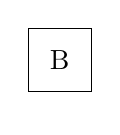
\begin{tikzpicture}
  \filldraw[fill=white!0, draw=none] (0cm,0cm) rectangle (0.8cm, -1cm);
  \filldraw[fill=white] (0cm,-0.8cm) rectangle (0.8cm,0cm);
  \node at (0.4cm,-0.4cm) {B};
\end{tikzpicture}
\end{center}
\noindent\rule{\linewidth}{0.3pt}
\begin{center}
\begin{flushleft}\textbf{Closed Set}\\[1.75mm]\end{flushleft}
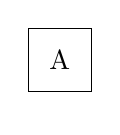
\begin{tikzpicture}
  \filldraw[fill=white!0, draw=none] (0cm,0cm) rectangle (0.8cm, -1cm);
  \filldraw[fill=white] (0cm,-0.8cm) rectangle (0.8cm,0cm);
  \node at (0.4cm,-0.4cm) {A};
\end{tikzpicture}
\end{center}
\noindent\rule{\linewidth}{0.3pt}
\begin{center}
\begin{flushleft}\textbf{Node Costs}\\[1.75mm]\end{flushleft}
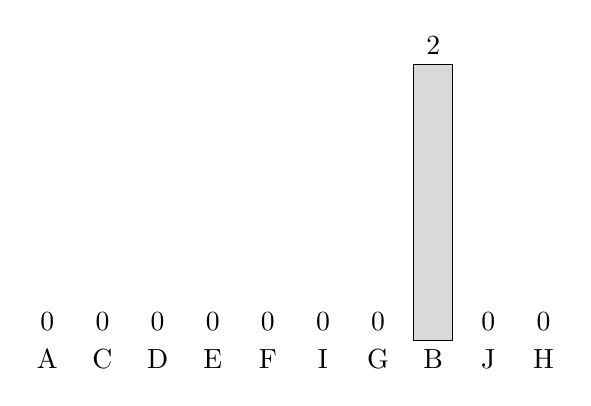
\begin{tikzpicture}
  \filldraw[fill=white!0, draw=none] (0cm,0) rectangle (0.5cm,3.5cm);
  \node[above] at (0.25cm,0cm) {0};
  \node[below] at (0.25cm,0) {A};
  \filldraw[fill=white!0, draw=none] (0.7cm,0) rectangle (1.2cm,3.5cm);
  \node[above] at (0.95cm,0cm) {0};
  \node[below] at (0.95cm,0) {C};
  \filldraw[fill=white!0, draw=none] (1.4cm,0) rectangle (1.9cm,3.5cm);
  \node[above] at (1.65cm,0cm) {0};
  \node[below] at (1.65cm,0) {D};
  \filldraw[fill=white!0, draw=none] (2.0999999999999996cm,0) rectangle (2.5999999999999996cm,3.5cm);
  \node[above] at (2.3499999999999996cm,0cm) {0};
  \node[below] at (2.3499999999999996cm,0) {E};
  \filldraw[fill=white!0, draw=none] (2.8cm,0) rectangle (3.3cm,3.5cm);
  \node[above] at (3.05cm,0cm) {0};
  \node[below] at (3.05cm,0) {F};
  \filldraw[fill=white!0, draw=none] (3.5cm,0) rectangle (4cm,3.5cm);
  \node[above] at (3.75cm,0cm) {0};
  \node[below] at (3.75cm,0) {I};
  \filldraw[fill=white!0, draw=none] (4.199999999999999cm,0) rectangle (4.699999999999999cm,3.5cm);
  \node[above] at (4.449999999999999cm,0cm) {0};
  \node[below] at (4.449999999999999cm,0) {G};
  \filldraw[fill=white!0, draw=none] (4.8999999999999995cm,0) rectangle (5.3999999999999995cm,3.5cm);
  \filldraw[fill=gray!30] (4.8999999999999995cm,0) rectangle (5.3999999999999995cm,3.5cm);
  \node[above] at (5.1499999999999995cm,3.5cm) {2};
  \node[below] at (5.1499999999999995cm,0) {B};
  \filldraw[fill=white!0, draw=none] (5.6cm,0) rectangle (6.1cm,3.5cm);
  \node[above] at (5.85cm,0cm) {0};
  \node[below] at (5.85cm,0) {J};
  \filldraw[fill=white!0, draw=none] (6.3cm,0) rectangle (6.8cm,3.5cm);
  \node[above] at (6.55cm,0cm) {0};
  \node[below] at (6.55cm,0) {H};
\end{tikzpicture}
\end{center}
\newpage
% --- Frame 7 ---
\begin{center}\LARGE\textbf{A* Algorithm}\\[6mm]\end{center}
\begin{center}
\begin{flushleft}\textbf{Log}\\[1.75mm]\end{flushleft}

\begin{tikzpicture}
  \filldraw[fill=white!0, draw=none] (0,0) rectangle (10cm, -0.25cm);
  \node[anchor=north, align=center, text=black] at (5cm,0) {\texttt{Adding neighbor C to open set}};
\end{tikzpicture}
\end{center}
\noindent\rule{\linewidth}{0.3pt}
\begin{center}
\begin{flushleft}\textbf{Graph}\\[2mm]\end{flushleft}
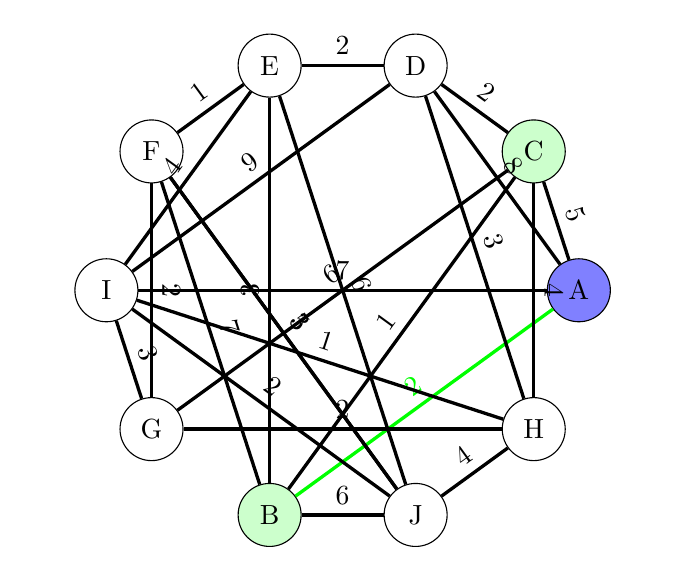
\begin{tikzpicture}
  \filldraw[fill=white!0, draw=none] (-4cm,0) rectangle (4cm, -3cm);
  \node[circle, draw, minimum size=8mm, fill=blue!50] (A) at (0.0:3cm) {A};
  \node[circle, draw, minimum size=8mm, fill=green!20] (C) at (36.0:3cm) {C};
  \node[circle, draw, minimum size=8mm, fill=white] (D) at (72.0:3cm) {D};
  \node[circle, draw, minimum size=8mm, fill=white] (E) at (108.0:3cm) {E};
  \node[circle, draw, minimum size=8mm, fill=white] (F) at (144.0:3cm) {F};
  \node[circle, draw, minimum size=8mm, fill=white] (I) at (180.0:3cm) {I};
  \node[circle, draw, minimum size=8mm, fill=white] (G) at (216.0:3cm) {G};
  \node[circle, draw, minimum size=8mm, fill=green!20] (B) at (252.0:3cm) {B};
  \node[circle, draw, minimum size=8mm, fill=white] (J) at (288.0:3cm) {J};
  \node[circle, draw, minimum size=8mm, fill=white] (H) at (324.0:3cm) {H};
  \draw[green!100, line width=1.2pt] (A) -- node[midway, sloped, above] {2} (B);
  \draw[black, line width=1.2pt] (A) -- node[midway, sloped, above] {5} (C);
  \draw[black, line width=1.2pt] (A) -- node[midway, sloped, above] {8} (D);
  \draw[black, line width=1.2pt] (C) -- node[midway, sloped, above] {2} (D);
  \draw[black, line width=1.2pt] (C) -- node[midway, sloped, above] {6} (G);
  \draw[black, line width=1.2pt] (C) -- node[midway, sloped, above] {4} (H);
  \draw[black, line width=1.2pt] (D) -- node[midway, sloped, above] {2} (E);
  \draw[black, line width=1.2pt] (D) -- node[midway, sloped, above] {3} (H);
  \draw[black, line width=1.2pt] (D) -- node[midway, sloped, above] {9} (I);
  \draw[black, line width=1.2pt] (E) -- node[midway, sloped, above] {1} (F);
  \draw[black, line width=1.2pt] (E) -- node[midway, sloped, above] {4} (I);
  \draw[black, line width=1.2pt] (E) -- node[midway, sloped, above] {6} (J);
  \draw[black, line width=1.2pt] (F) -- node[midway, sloped, above] {2} (G);
  \draw[black, line width=1.2pt] (F) -- node[midway, sloped, above] {5} (J);
  \draw[black, line width=1.2pt] (I) -- node[midway, sloped, above] {2} (J);
  \draw[black, line width=1.2pt] (I) -- node[midway, sloped, above] {7} (A);
  \draw[black, line width=1.2pt] (G) -- node[midway, sloped, above] {2} (H);
  \draw[black, line width=1.2pt] (G) -- node[midway, sloped, above] {3} (I);
  \draw[black, line width=1.2pt] (B) -- node[midway, sloped, above] {1} (C);
  \draw[black, line width=1.2pt] (B) -- node[midway, sloped, above] {3} (E);
  \draw[black, line width=1.2pt] (B) -- node[midway, sloped, above] {7} (F);
  \draw[black, line width=1.2pt] (J) -- node[midway, sloped, above] {6} (B);
  \draw[black, line width=1.2pt] (J) -- node[midway, sloped, above] {3} (F);
  \draw[black, line width=1.2pt] (H) -- node[midway, sloped, above] {1} (I);
  \draw[black, line width=1.2pt] (H) -- node[midway, sloped, above] {4} (J);
\end{tikzpicture}
\end{center}
\noindent\rule{\linewidth}{0.3pt}
\begin{center}
\begin{flushleft}\textbf{Open Set}\\[1.75mm]\end{flushleft}
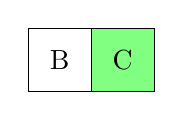
\begin{tikzpicture}
  \filldraw[fill=white!0, draw=none] (0cm,0cm) rectangle (1.6cm, -1cm);
  \filldraw[fill=white] (0cm,-0.8cm) rectangle (0.8cm,0cm);
  \node at (0.4cm,-0.4cm) {B};
  \filldraw[fill=green!50] (0.8cm,-0.8cm) rectangle (1.6cm,0cm);
  \node at (1.2000000000000002cm,-0.4cm) {C};
\end{tikzpicture}
\end{center}
\noindent\rule{\linewidth}{0.3pt}
\begin{center}
\begin{flushleft}\textbf{Closed Set}\\[1.75mm]\end{flushleft}
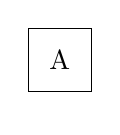
\begin{tikzpicture}
  \filldraw[fill=white!0, draw=none] (0cm,0cm) rectangle (0.8cm, -1cm);
  \filldraw[fill=white] (0cm,-0.8cm) rectangle (0.8cm,0cm);
  \node at (0.4cm,-0.4cm) {A};
\end{tikzpicture}
\end{center}
\noindent\rule{\linewidth}{0.3pt}
\begin{center}
\begin{flushleft}\textbf{Node Costs}\\[1.75mm]\end{flushleft}
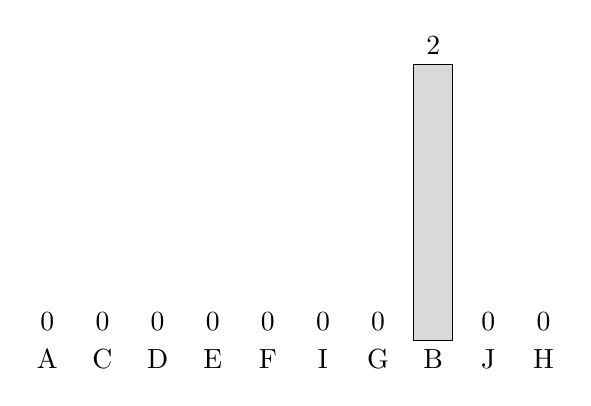
\begin{tikzpicture}
  \filldraw[fill=white!0, draw=none] (0cm,0) rectangle (0.5cm,3.5cm);
  \node[above] at (0.25cm,0cm) {0};
  \node[below] at (0.25cm,0) {A};
  \filldraw[fill=white!0, draw=none] (0.7cm,0) rectangle (1.2cm,3.5cm);
  \node[above] at (0.95cm,0cm) {0};
  \node[below] at (0.95cm,0) {C};
  \filldraw[fill=white!0, draw=none] (1.4cm,0) rectangle (1.9cm,3.5cm);
  \node[above] at (1.65cm,0cm) {0};
  \node[below] at (1.65cm,0) {D};
  \filldraw[fill=white!0, draw=none] (2.0999999999999996cm,0) rectangle (2.5999999999999996cm,3.5cm);
  \node[above] at (2.3499999999999996cm,0cm) {0};
  \node[below] at (2.3499999999999996cm,0) {E};
  \filldraw[fill=white!0, draw=none] (2.8cm,0) rectangle (3.3cm,3.5cm);
  \node[above] at (3.05cm,0cm) {0};
  \node[below] at (3.05cm,0) {F};
  \filldraw[fill=white!0, draw=none] (3.5cm,0) rectangle (4cm,3.5cm);
  \node[above] at (3.75cm,0cm) {0};
  \node[below] at (3.75cm,0) {I};
  \filldraw[fill=white!0, draw=none] (4.199999999999999cm,0) rectangle (4.699999999999999cm,3.5cm);
  \node[above] at (4.449999999999999cm,0cm) {0};
  \node[below] at (4.449999999999999cm,0) {G};
  \filldraw[fill=white!0, draw=none] (4.8999999999999995cm,0) rectangle (5.3999999999999995cm,3.5cm);
  \filldraw[fill=gray!30] (4.8999999999999995cm,0) rectangle (5.3999999999999995cm,3.5cm);
  \node[above] at (5.1499999999999995cm,3.5cm) {2};
  \node[below] at (5.1499999999999995cm,0) {B};
  \filldraw[fill=white!0, draw=none] (5.6cm,0) rectangle (6.1cm,3.5cm);
  \node[above] at (5.85cm,0cm) {0};
  \node[below] at (5.85cm,0) {J};
  \filldraw[fill=white!0, draw=none] (6.3cm,0) rectangle (6.8cm,3.5cm);
  \node[above] at (6.55cm,0cm) {0};
  \node[below] at (6.55cm,0) {H};
\end{tikzpicture}
\end{center}
\newpage
% --- Frame 8 ---
\begin{center}\LARGE\textbf{A* Algorithm}\\[6mm]\end{center}
\begin{center}
\begin{flushleft}\textbf{Log}\\[1.75mm]\end{flushleft}

\begin{tikzpicture}
  \filldraw[fill=white!0, draw=none] (0,0) rectangle (10cm, -0.25cm);
  \node[anchor=north, align=center, text=black] at (5cm,0) {\texttt{Updating cost for neighbor C (cost: 5)}};
\end{tikzpicture}
\end{center}
\noindent\rule{\linewidth}{0.3pt}
\begin{center}
\begin{flushleft}\textbf{Graph}\\[2mm]\end{flushleft}
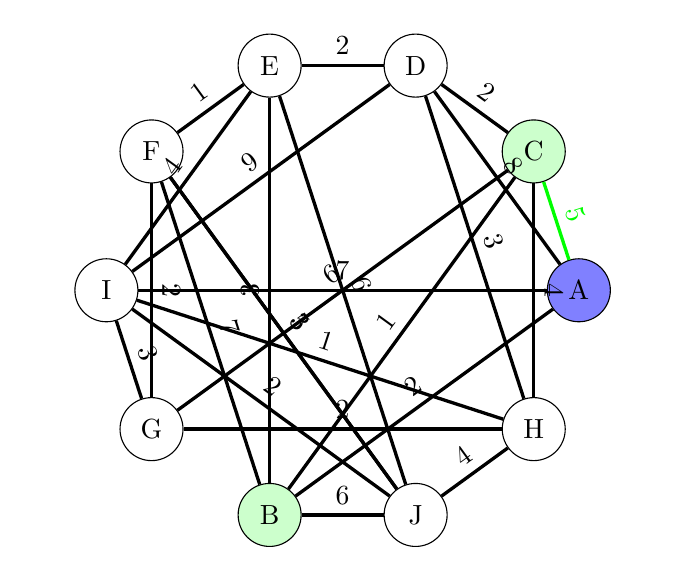
\begin{tikzpicture}
  \filldraw[fill=white!0, draw=none] (-4cm,0) rectangle (4cm, -3cm);
  \node[circle, draw, minimum size=8mm, fill=blue!50] (A) at (0.0:3cm) {A};
  \node[circle, draw, minimum size=8mm, fill=green!20] (C) at (36.0:3cm) {C};
  \node[circle, draw, minimum size=8mm, fill=white] (D) at (72.0:3cm) {D};
  \node[circle, draw, minimum size=8mm, fill=white] (E) at (108.0:3cm) {E};
  \node[circle, draw, minimum size=8mm, fill=white] (F) at (144.0:3cm) {F};
  \node[circle, draw, minimum size=8mm, fill=white] (I) at (180.0:3cm) {I};
  \node[circle, draw, minimum size=8mm, fill=white] (G) at (216.0:3cm) {G};
  \node[circle, draw, minimum size=8mm, fill=green!20] (B) at (252.0:3cm) {B};
  \node[circle, draw, minimum size=8mm, fill=white] (J) at (288.0:3cm) {J};
  \node[circle, draw, minimum size=8mm, fill=white] (H) at (324.0:3cm) {H};
  \draw[black, line width=1.2pt] (A) -- node[midway, sloped, above] {2} (B);
  \draw[green!100, line width=1.2pt] (A) -- node[midway, sloped, above] {5} (C);
  \draw[black, line width=1.2pt] (A) -- node[midway, sloped, above] {8} (D);
  \draw[black, line width=1.2pt] (C) -- node[midway, sloped, above] {2} (D);
  \draw[black, line width=1.2pt] (C) -- node[midway, sloped, above] {6} (G);
  \draw[black, line width=1.2pt] (C) -- node[midway, sloped, above] {4} (H);
  \draw[black, line width=1.2pt] (D) -- node[midway, sloped, above] {2} (E);
  \draw[black, line width=1.2pt] (D) -- node[midway, sloped, above] {3} (H);
  \draw[black, line width=1.2pt] (D) -- node[midway, sloped, above] {9} (I);
  \draw[black, line width=1.2pt] (E) -- node[midway, sloped, above] {1} (F);
  \draw[black, line width=1.2pt] (E) -- node[midway, sloped, above] {4} (I);
  \draw[black, line width=1.2pt] (E) -- node[midway, sloped, above] {6} (J);
  \draw[black, line width=1.2pt] (F) -- node[midway, sloped, above] {2} (G);
  \draw[black, line width=1.2pt] (F) -- node[midway, sloped, above] {5} (J);
  \draw[black, line width=1.2pt] (I) -- node[midway, sloped, above] {2} (J);
  \draw[black, line width=1.2pt] (I) -- node[midway, sloped, above] {7} (A);
  \draw[black, line width=1.2pt] (G) -- node[midway, sloped, above] {2} (H);
  \draw[black, line width=1.2pt] (G) -- node[midway, sloped, above] {3} (I);
  \draw[black, line width=1.2pt] (B) -- node[midway, sloped, above] {1} (C);
  \draw[black, line width=1.2pt] (B) -- node[midway, sloped, above] {3} (E);
  \draw[black, line width=1.2pt] (B) -- node[midway, sloped, above] {7} (F);
  \draw[black, line width=1.2pt] (J) -- node[midway, sloped, above] {6} (B);
  \draw[black, line width=1.2pt] (J) -- node[midway, sloped, above] {3} (F);
  \draw[black, line width=1.2pt] (H) -- node[midway, sloped, above] {1} (I);
  \draw[black, line width=1.2pt] (H) -- node[midway, sloped, above] {4} (J);
\end{tikzpicture}
\end{center}
\noindent\rule{\linewidth}{0.3pt}
\begin{center}
\begin{flushleft}\textbf{Open Set}\\[1.75mm]\end{flushleft}
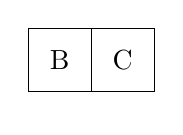
\begin{tikzpicture}
  \filldraw[fill=white!0, draw=none] (0cm,0cm) rectangle (1.6cm, -1cm);
  \filldraw[fill=white] (0cm,-0.8cm) rectangle (0.8cm,0cm);
  \node at (0.4cm,-0.4cm) {B};
  \filldraw[fill=white] (0.8cm,-0.8cm) rectangle (1.6cm,0cm);
  \node at (1.2000000000000002cm,-0.4cm) {C};
\end{tikzpicture}
\end{center}
\noindent\rule{\linewidth}{0.3pt}
\begin{center}
\begin{flushleft}\textbf{Closed Set}\\[1.75mm]\end{flushleft}
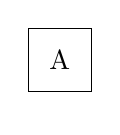
\begin{tikzpicture}
  \filldraw[fill=white!0, draw=none] (0cm,0cm) rectangle (0.8cm, -1cm);
  \filldraw[fill=white] (0cm,-0.8cm) rectangle (0.8cm,0cm);
  \node at (0.4cm,-0.4cm) {A};
\end{tikzpicture}
\end{center}
\noindent\rule{\linewidth}{0.3pt}
\begin{center}
\begin{flushleft}\textbf{Node Costs}\\[1.75mm]\end{flushleft}
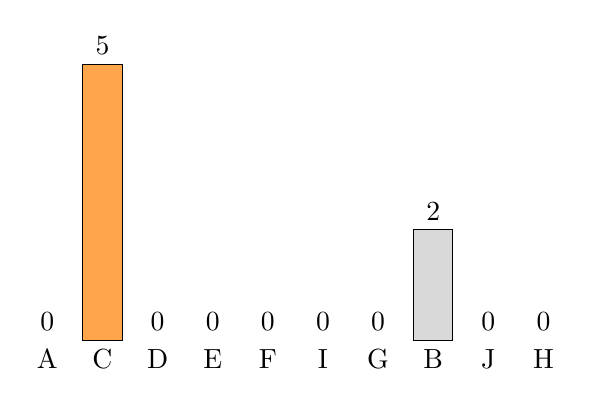
\begin{tikzpicture}
  \filldraw[fill=white!0, draw=none] (0cm,0) rectangle (0.5cm,3.5cm);
  \node[above] at (0.25cm,0cm) {0};
  \node[below] at (0.25cm,0) {A};
  \filldraw[fill=white!0, draw=none] (0.7cm,0) rectangle (1.2cm,3.5cm);
  \filldraw[fill=orange!70] (0.7cm,0cm) rectangle (1.2cm,3.5cm);
  \node[above] at (0.95cm,3.5cm) {5};
  \node[below] at (0.95cm,0) {C};
  \filldraw[fill=white!0, draw=none] (1.4cm,0) rectangle (1.9cm,3.5cm);
  \node[above] at (1.65cm,0cm) {0};
  \node[below] at (1.65cm,0) {D};
  \filldraw[fill=white!0, draw=none] (2.0999999999999996cm,0) rectangle (2.5999999999999996cm,3.5cm);
  \node[above] at (2.3499999999999996cm,0cm) {0};
  \node[below] at (2.3499999999999996cm,0) {E};
  \filldraw[fill=white!0, draw=none] (2.8cm,0) rectangle (3.3cm,3.5cm);
  \node[above] at (3.05cm,0cm) {0};
  \node[below] at (3.05cm,0) {F};
  \filldraw[fill=white!0, draw=none] (3.5cm,0) rectangle (4cm,3.5cm);
  \node[above] at (3.75cm,0cm) {0};
  \node[below] at (3.75cm,0) {I};
  \filldraw[fill=white!0, draw=none] (4.199999999999999cm,0) rectangle (4.699999999999999cm,3.5cm);
  \node[above] at (4.449999999999999cm,0cm) {0};
  \node[below] at (4.449999999999999cm,0) {G};
  \filldraw[fill=white!0, draw=none] (4.8999999999999995cm,0) rectangle (5.3999999999999995cm,3.5cm);
  \filldraw[fill=gray!30] (4.8999999999999995cm,0) rectangle (5.3999999999999995cm,1.4cm);
  \node[above] at (5.1499999999999995cm,1.4cm) {2};
  \node[below] at (5.1499999999999995cm,0) {B};
  \filldraw[fill=white!0, draw=none] (5.6cm,0) rectangle (6.1cm,3.5cm);
  \node[above] at (5.85cm,0cm) {0};
  \node[below] at (5.85cm,0) {J};
  \filldraw[fill=white!0, draw=none] (6.3cm,0) rectangle (6.8cm,3.5cm);
  \node[above] at (6.55cm,0cm) {0};
  \node[below] at (6.55cm,0) {H};
\end{tikzpicture}
\end{center}
\newpage
% --- Frame 9 ---
\begin{center}\LARGE\textbf{A* Algorithm}\\[6mm]\end{center}
\begin{center}
\begin{flushleft}\textbf{Log}\\[1.75mm]\end{flushleft}

\begin{tikzpicture}
  \filldraw[fill=white!0, draw=none] (0,0) rectangle (10cm, -0.25cm);
  \node[anchor=north, align=center, text=black] at (5cm,0) {\texttt{Checking neighbor D}};
\end{tikzpicture}
\end{center}
\noindent\rule{\linewidth}{0.3pt}
\begin{center}
\begin{flushleft}\textbf{Graph}\\[2mm]\end{flushleft}
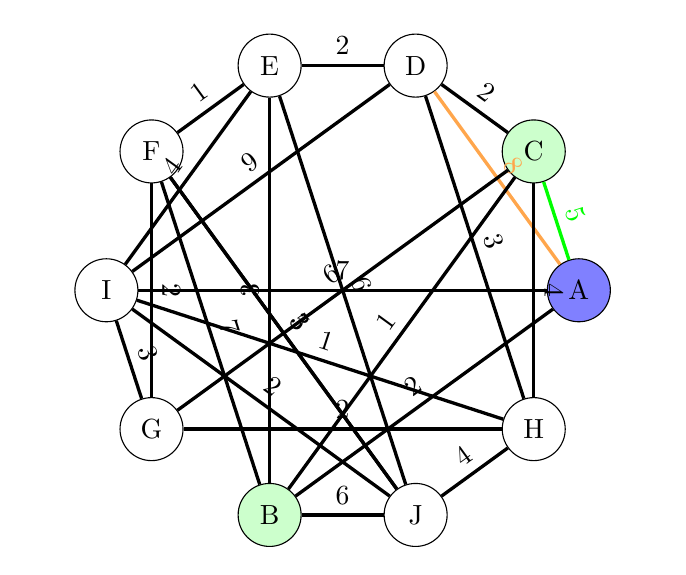
\begin{tikzpicture}
  \filldraw[fill=white!0, draw=none] (-4cm,0) rectangle (4cm, -3cm);
  \node[circle, draw, minimum size=8mm, fill=blue!50] (A) at (0.0:3cm) {A};
  \node[circle, draw, minimum size=8mm, fill=green!20] (C) at (36.0:3cm) {C};
  \node[circle, draw, minimum size=8mm, fill=white] (D) at (72.0:3cm) {D};
  \node[circle, draw, minimum size=8mm, fill=white] (E) at (108.0:3cm) {E};
  \node[circle, draw, minimum size=8mm, fill=white] (F) at (144.0:3cm) {F};
  \node[circle, draw, minimum size=8mm, fill=white] (I) at (180.0:3cm) {I};
  \node[circle, draw, minimum size=8mm, fill=white] (G) at (216.0:3cm) {G};
  \node[circle, draw, minimum size=8mm, fill=green!20] (B) at (252.0:3cm) {B};
  \node[circle, draw, minimum size=8mm, fill=white] (J) at (288.0:3cm) {J};
  \node[circle, draw, minimum size=8mm, fill=white] (H) at (324.0:3cm) {H};
  \draw[black, line width=1.2pt] (A) -- node[midway, sloped, above] {2} (B);
  \draw[green!100, line width=1.2pt] (A) -- node[midway, sloped, above] {5} (C);
  \draw[orange!70, line width=1.2pt] (A) -- node[midway, sloped, above] {8} (D);
  \draw[black, line width=1.2pt] (C) -- node[midway, sloped, above] {2} (D);
  \draw[black, line width=1.2pt] (C) -- node[midway, sloped, above] {6} (G);
  \draw[black, line width=1.2pt] (C) -- node[midway, sloped, above] {4} (H);
  \draw[black, line width=1.2pt] (D) -- node[midway, sloped, above] {2} (E);
  \draw[black, line width=1.2pt] (D) -- node[midway, sloped, above] {3} (H);
  \draw[black, line width=1.2pt] (D) -- node[midway, sloped, above] {9} (I);
  \draw[black, line width=1.2pt] (E) -- node[midway, sloped, above] {1} (F);
  \draw[black, line width=1.2pt] (E) -- node[midway, sloped, above] {4} (I);
  \draw[black, line width=1.2pt] (E) -- node[midway, sloped, above] {6} (J);
  \draw[black, line width=1.2pt] (F) -- node[midway, sloped, above] {2} (G);
  \draw[black, line width=1.2pt] (F) -- node[midway, sloped, above] {5} (J);
  \draw[black, line width=1.2pt] (I) -- node[midway, sloped, above] {2} (J);
  \draw[black, line width=1.2pt] (I) -- node[midway, sloped, above] {7} (A);
  \draw[black, line width=1.2pt] (G) -- node[midway, sloped, above] {2} (H);
  \draw[black, line width=1.2pt] (G) -- node[midway, sloped, above] {3} (I);
  \draw[black, line width=1.2pt] (B) -- node[midway, sloped, above] {1} (C);
  \draw[black, line width=1.2pt] (B) -- node[midway, sloped, above] {3} (E);
  \draw[black, line width=1.2pt] (B) -- node[midway, sloped, above] {7} (F);
  \draw[black, line width=1.2pt] (J) -- node[midway, sloped, above] {6} (B);
  \draw[black, line width=1.2pt] (J) -- node[midway, sloped, above] {3} (F);
  \draw[black, line width=1.2pt] (H) -- node[midway, sloped, above] {1} (I);
  \draw[black, line width=1.2pt] (H) -- node[midway, sloped, above] {4} (J);
\end{tikzpicture}
\end{center}
\noindent\rule{\linewidth}{0.3pt}
\begin{center}
\begin{flushleft}\textbf{Open Set}\\[1.75mm]\end{flushleft}
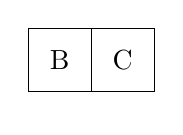
\begin{tikzpicture}
  \filldraw[fill=white!0, draw=none] (0cm,0cm) rectangle (1.6cm, -1cm);
  \filldraw[fill=white] (0cm,-0.8cm) rectangle (0.8cm,0cm);
  \node at (0.4cm,-0.4cm) {B};
  \filldraw[fill=white] (0.8cm,-0.8cm) rectangle (1.6cm,0cm);
  \node at (1.2000000000000002cm,-0.4cm) {C};
\end{tikzpicture}
\end{center}
\noindent\rule{\linewidth}{0.3pt}
\begin{center}
\begin{flushleft}\textbf{Closed Set}\\[1.75mm]\end{flushleft}
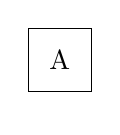
\begin{tikzpicture}
  \filldraw[fill=white!0, draw=none] (0cm,0cm) rectangle (0.8cm, -1cm);
  \filldraw[fill=white] (0cm,-0.8cm) rectangle (0.8cm,0cm);
  \node at (0.4cm,-0.4cm) {A};
\end{tikzpicture}
\end{center}
\noindent\rule{\linewidth}{0.3pt}
\begin{center}
\begin{flushleft}\textbf{Node Costs}\\[1.75mm]\end{flushleft}
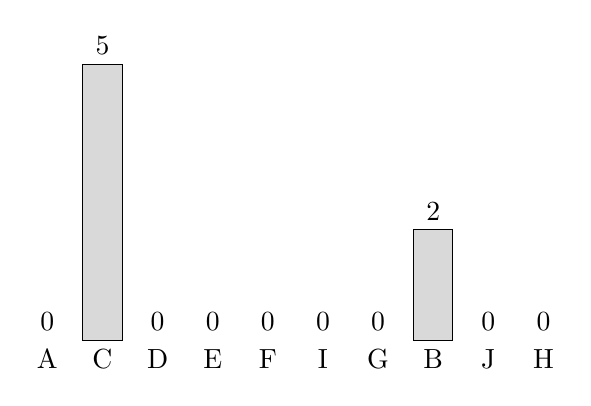
\begin{tikzpicture}
  \filldraw[fill=white!0, draw=none] (0cm,0) rectangle (0.5cm,3.5cm);
  \node[above] at (0.25cm,0cm) {0};
  \node[below] at (0.25cm,0) {A};
  \filldraw[fill=white!0, draw=none] (0.7cm,0) rectangle (1.2cm,3.5cm);
  \filldraw[fill=gray!30] (0.7cm,0) rectangle (1.2cm,3.5cm);
  \node[above] at (0.95cm,3.5cm) {5};
  \node[below] at (0.95cm,0) {C};
  \filldraw[fill=white!0, draw=none] (1.4cm,0) rectangle (1.9cm,3.5cm);
  \node[above] at (1.65cm,0cm) {0};
  \node[below] at (1.65cm,0) {D};
  \filldraw[fill=white!0, draw=none] (2.0999999999999996cm,0) rectangle (2.5999999999999996cm,3.5cm);
  \node[above] at (2.3499999999999996cm,0cm) {0};
  \node[below] at (2.3499999999999996cm,0) {E};
  \filldraw[fill=white!0, draw=none] (2.8cm,0) rectangle (3.3cm,3.5cm);
  \node[above] at (3.05cm,0cm) {0};
  \node[below] at (3.05cm,0) {F};
  \filldraw[fill=white!0, draw=none] (3.5cm,0) rectangle (4cm,3.5cm);
  \node[above] at (3.75cm,0cm) {0};
  \node[below] at (3.75cm,0) {I};
  \filldraw[fill=white!0, draw=none] (4.199999999999999cm,0) rectangle (4.699999999999999cm,3.5cm);
  \node[above] at (4.449999999999999cm,0cm) {0};
  \node[below] at (4.449999999999999cm,0) {G};
  \filldraw[fill=white!0, draw=none] (4.8999999999999995cm,0) rectangle (5.3999999999999995cm,3.5cm);
  \filldraw[fill=gray!30] (4.8999999999999995cm,0) rectangle (5.3999999999999995cm,1.4cm);
  \node[above] at (5.1499999999999995cm,1.4cm) {2};
  \node[below] at (5.1499999999999995cm,0) {B};
  \filldraw[fill=white!0, draw=none] (5.6cm,0) rectangle (6.1cm,3.5cm);
  \node[above] at (5.85cm,0cm) {0};
  \node[below] at (5.85cm,0) {J};
  \filldraw[fill=white!0, draw=none] (6.3cm,0) rectangle (6.8cm,3.5cm);
  \node[above] at (6.55cm,0cm) {0};
  \node[below] at (6.55cm,0) {H};
\end{tikzpicture}
\end{center}
\newpage
% --- Frame 10 ---
\begin{center}\LARGE\textbf{A* Algorithm}\\[6mm]\end{center}
\begin{center}
\begin{flushleft}\textbf{Log}\\[1.75mm]\end{flushleft}
\begin{tikzpicture}
  \filldraw[fill=white!0, draw=none] (0,0) rectangle (10cm, -0.25cm);
  \node[anchor=north, align=center, text=black] at (5cm,0) {\texttt{Adding neighbor D to open set}};
\end{tikzpicture}
\end{center}
\noindent\rule{\linewidth}{0.3pt}
\begin{center}
\begin{flushleft}\textbf{Graph}\\[2mm]\end{flushleft}
\begin{tikzpicture}
  \filldraw[fill=white!0, draw=none] (-4cm,0) rectangle (4cm, -3cm);
  \node[circle, draw, minimum size=8mm, fill=blue!50] (A) at (0.0:3cm) {A};
  \node[circle, draw, minimum size=8mm, fill=green!20] (C) at (36.0:3cm) {C};
  \node[circle, draw, minimum size=8mm, fill=green!20] (D) at (72.0:3cm) {D};
  \node[circle, draw, minimum size=8mm, fill=white] (E) at (108.0:3cm) {E};
  \node[circle, draw, minimum size=8mm, fill=white] (F) at (144.0:3cm) {F};
  \node[circle, draw, minimum size=8mm, fill=white] (I) at (180.0:3cm) {I};
  \node[circle, draw, minimum size=8mm, fill=white] (G) at (216.0:3cm) {G};
  \node[circle, draw, minimum size=8mm, fill=green!20] (B) at (252.0:3cm) {B};
  \node[circle, draw, minimum size=8mm, fill=white] (J) at (288.0:3cm) {J};
  \node[circle, draw, minimum size=8mm, fill=white] (H) at (324.0:3cm) {H};
  \draw[black, line width=1.2pt] (A) -- node[midway, sloped, above] {2} (B);
  \draw[green!100, line width=1.2pt] (A) -- node[midway, sloped, above] {5} (C);
  \draw[black, line width=1.2pt] (A) -- node[midway, sloped, above] {8} (D);
  \draw[black, line width=1.2pt] (C) -- node[midway, sloped, above] {2} (D);
  \draw[black, line width=1.2pt] (C) -- node[midway, sloped, above] {6} (G);
  \draw[black, line width=1.2pt] (C) -- node[midway, sloped, above] {4} (H);
  \draw[black, line width=1.2pt] (D) -- node[midway, sloped, above] {2} (E);
  \draw[black, line width=1.2pt] (D) -- node[midway, sloped, above] {3} (H);
  \draw[black, line width=1.2pt] (D) -- node[midway, sloped, above] {9} (I);
  \draw[black, line width=1.2pt] (E) -- node[midway, sloped, above] {1} (F);
  \draw[black, line width=1.2pt] (E) -- node[midway, sloped, above] {4} (I);
  \draw[black, line width=1.2pt] (E) -- node[midway, sloped, above] {6} (J);
  \draw[black, line width=1.2pt] (F) -- node[midway, sloped, above] {2} (G);
  \draw[black, line width=1.2pt] (F) -- node[midway, sloped, above] {5} (J);
  \draw[black, line width=1.2pt] (I) -- node[midway, sloped, above] {2} (J);
  \draw[black, line width=1.2pt] (I) -- node[midway, sloped, above] {7} (A);
  \draw[black, line width=1.2pt] (G) -- node[midway, sloped, above] {2} (H);
  \draw[black, line width=1.2pt] (G) -- node[midway, sloped, above] {3} (I);
  \draw[black, line width=1.2pt] (B) -- node[midway, sloped, above] {1} (C);
  \draw[black, line width=1.2pt] (B) -- node[midway, sloped, above] {3} (E);
  \draw[black, line width=1.2pt] (B) -- node[midway, sloped, above] {7} (F);
  \draw[black, line width=1.2pt] (J) -- node[midway, sloped, above] {6} (B);
  \draw[black, line width=1.2pt] (J) -- node[midway, sloped, above] {3} (F);
  \draw[black, line width=1.2pt] (H) -- node[midway, sloped, above] {1} (I);
  \draw[black, line width=1.2pt] (H) -- node[midway, sloped, above] {4} (J);
\end{tikzpicture}
\end{center}
\noindent\rule{\linewidth}{0.3pt}
\begin{center}
\begin{flushleft}\textbf{Open Set}\\[1.75mm]\end{flushleft}
\begin{tikzpicture}
  \filldraw[fill=white!0, draw=none] (0cm,0cm) rectangle (2.4000000000000004cm, -1cm);
  \filldraw[fill=white] (0cm,-0.8cm) rectangle (0.8cm,0cm);
  \node at (0.4cm,-0.4cm) {B};
  \filldraw[fill=white] (0.8cm,-0.8cm) rectangle (1.6cm,0cm);
  \node at (1.2000000000000002cm,-0.4cm) {C};
  \filldraw[fill=green!50] (1.6cm,-0.8cm) rectangle (2.4000000000000004cm,0cm);
  \node at (2cm,-0.4cm) {D};
\end{tikzpicture}
\end{center}
\noindent\rule{\linewidth}{0.3pt}
\begin{center}
\begin{flushleft}\textbf{Closed Set}\\[1.75mm]\end{flushleft}
\begin{tikzpicture}
  \filldraw[fill=white!0, draw=none] (0cm,0cm) rectangle (0.8cm, -1cm);
  \filldraw[fill=white] (0cm,-0.8cm) rectangle (0.8cm,0cm);
  \node at (0.4cm,-0.4cm) {A};
\end{tikzpicture}
\end{center}
\noindent\rule{\linewidth}{0.3pt}
\begin{center}
\begin{flushleft}\textbf{Node Costs}\\[1.75mm]\end{flushleft}
\begin{tikzpicture}
  \filldraw[fill=white!0, draw=none] (0cm,0) rectangle (0.5cm,3.5cm);
  \node[above] at (0.25cm,0cm) {0};
  \node[below] at (0.25cm,0) {A};
  \filldraw[fill=white!0, draw=none] (0.7cm,0) rectangle (1.2cm,3.5cm);
  \filldraw[fill=gray!30] (0.7cm,0) rectangle (1.2cm,3.5cm);
  \node[above] at (0.95cm,3.5cm) {5};
  \node[below] at (0.95cm,0) {C};
  \filldraw[fill=white!0, draw=none] (1.4cm,0) rectangle (1.9cm,3.5cm);
  \node[above] at (1.65cm,0cm) {0};
  \node[below] at (1.65cm,0) {D};
  \filldraw[fill=white!0, draw=none] (2.0999999999999996cm,0) rectangle (2.5999999999999996cm,3.5cm);
  \node[above] at (2.3499999999999996cm,0cm) {0};
  \node[below] at (2.3499999999999996cm,0) {E};
  \filldraw[fill=white!0, draw=none] (2.8cm,0) rectangle (3.3cm,3.5cm);
  \node[above] at (3.05cm,0cm) {0};
  \node[below] at (3.05cm,0) {F};
  \filldraw[fill=white!0, draw=none] (3.5cm,0) rectangle (4cm,3.5cm);
  \node[above] at (3.75cm,0cm) {0};
  \node[below] at (3.75cm,0) {I};
  \filldraw[fill=white!0, draw=none] (4.199999999999999cm,0) rectangle (4.699999999999999cm,3.5cm);
  \node[above] at (4.449999999999999cm,0cm) {0};
  \node[below] at (4.449999999999999cm,0) {G};
  \filldraw[fill=white!0, draw=none] (4.8999999999999995cm,0) rectangle (5.3999999999999995cm,3.5cm);
  \filldraw[fill=gray!30] (4.8999999999999995cm,0) rectangle (5.3999999999999995cm,1.4cm);
  \node[above] at (5.1499999999999995cm,1.4cm) {2};
  \node[below] at (5.1499999999999995cm,0) {B};
  \filldraw[fill=white!0, draw=none] (5.6cm,0) rectangle (6.1cm,3.5cm);
  \node[above] at (5.85cm,0cm) {0};
  \node[below] at (5.85cm,0) {J};
  \filldraw[fill=white!0, draw=none] (6.3cm,0) rectangle (6.8cm,3.5cm);
  \node[above] at (6.55cm,0cm) {0};
  \node[below] at (6.55cm,0) {H};
\end{tikzpicture}
\end{center}
\newpage
% --- Frame 11 ---
\begin{center}\LARGE\textbf{A* Algorithm}\\[6mm]\end{center}
\begin{center}
\begin{flushleft}\textbf{Log}\\[1.75mm]\end{flushleft}
\begin{tikzpicture}
  \filldraw[fill=white!0, draw=none] (0,0) rectangle (10cm, -0.25cm);
  \node[anchor=north, align=center, text=black] at (5cm,0) {\texttt{Updating cost for neighbor D (cost: 8)}};
\end{tikzpicture}
\end{center}
\noindent\rule{\linewidth}{0.3pt}
\begin{center}
\begin{flushleft}\textbf{Graph}\\[2mm]\end{flushleft}
\begin{tikzpicture}
  \filldraw[fill=white!0, draw=none] (-4cm,0) rectangle (4cm, -3cm);
  \node[circle, draw, minimum size=8mm, fill=blue!50] (A) at (0.0:3cm) {A};
  \node[circle, draw, minimum size=8mm, fill=green!20] (C) at (36.0:3cm) {C};
  \node[circle, draw, minimum size=8mm, fill=green!20] (D) at (72.0:3cm) {D};
  \node[circle, draw, minimum size=8mm, fill=white] (E) at (108.0:3cm) {E};
  \node[circle, draw, minimum size=8mm, fill=white] (F) at (144.0:3cm) {F};
  \node[circle, draw, minimum size=8mm, fill=white] (I) at (180.0:3cm) {I};
  \node[circle, draw, minimum size=8mm, fill=white] (G) at (216.0:3cm) {G};
  \node[circle, draw, minimum size=8mm, fill=green!20] (B) at (252.0:3cm) {B};
  \node[circle, draw, minimum size=8mm, fill=white] (J) at (288.0:3cm) {J};
  \node[circle, draw, minimum size=8mm, fill=white] (H) at (324.0:3cm) {H};
  \draw[black, line width=1.2pt] (A) -- node[midway, sloped, above] {2} (B);
  \draw[black, line width=1.2pt] (A) -- node[midway, sloped, above] {5} (C);
  \draw[green!100, line width=1.2pt] (A) -- node[midway, sloped, above] {8} (D);
  \draw[black, line width=1.2pt] (C) -- node[midway, sloped, above] {2} (D);
  \draw[black, line width=1.2pt] (C) -- node[midway, sloped, above] {6} (G);
  \draw[black, line width=1.2pt] (C) -- node[midway, sloped, above] {4} (H);
  \draw[black, line width=1.2pt] (D) -- node[midway, sloped, above] {2} (E);
  \draw[black, line width=1.2pt] (D) -- node[midway, sloped, above] {3} (H);
  \draw[black, line width=1.2pt] (D) -- node[midway, sloped, above] {9} (I);
  \draw[black, line width=1.2pt] (E) -- node[midway, sloped, above] {1} (F);
  \draw[black, line width=1.2pt] (E) -- node[midway, sloped, above] {4} (I);
  \draw[black, line width=1.2pt] (E) -- node[midway, sloped, above] {6} (J);
  \draw[black, line width=1.2pt] (F) -- node[midway, sloped, above] {2} (G);
  \draw[black, line width=1.2pt] (F) -- node[midway, sloped, above] {5} (J);
  \draw[black, line width=1.2pt] (I) -- node[midway, sloped, above] {2} (J);
  \draw[black, line width=1.2pt] (I) -- node[midway, sloped, above] {7} (A);
  \draw[black, line width=1.2pt] (G) -- node[midway, sloped, above] {2} (H);
  \draw[black, line width=1.2pt] (G) -- node[midway, sloped, above] {3} (I);
  \draw[black, line width=1.2pt] (B) -- node[midway, sloped, above] {1} (C);
  \draw[black, line width=1.2pt] (B) -- node[midway, sloped, above] {3} (E);
  \draw[black, line width=1.2pt] (B) -- node[midway, sloped, above] {7} (F);
  \draw[black, line width=1.2pt] (J) -- node[midway, sloped, above] {6} (B);
  \draw[black, line width=1.2pt] (J) -- node[midway, sloped, above] {3} (F);
  \draw[black, line width=1.2pt] (H) -- node[midway, sloped, above] {1} (I);
  \draw[black, line width=1.2pt] (H) -- node[midway, sloped, above] {4} (J);
\end{tikzpicture}
\end{center}
\noindent\rule{\linewidth}{0.3pt}
\begin{center}
\begin{flushleft}\textbf{Open Set}\\[1.75mm]\end{flushleft}
\begin{tikzpicture}
  \filldraw[fill=white!0, draw=none] (0cm,0cm) rectangle (2.4000000000000004cm, -1cm);
  \filldraw[fill=white] (0cm,-0.8cm) rectangle (0.8cm,0cm);
  \node at (0.4cm,-0.4cm) {B};
  \filldraw[fill=white] (0.8cm,-0.8cm) rectangle (1.6cm,0cm);
  \node at (1.2000000000000002cm,-0.4cm) {C};
  \filldraw[fill=white] (1.6cm,-0.8cm) rectangle (2.4000000000000004cm,0cm);
  \node at (2cm,-0.4cm) {D};
\end{tikzpicture}
\end{center}
\noindent\rule{\linewidth}{0.3pt}
\begin{center}
\begin{flushleft}\textbf{Closed Set}\\[1.75mm]\end{flushleft}
\begin{tikzpicture}
  \filldraw[fill=white!0, draw=none] (0cm,0cm) rectangle (0.8cm, -1cm);
  \filldraw[fill=white] (0cm,-0.8cm) rectangle (0.8cm,0cm);
  \node at (0.4cm,-0.4cm) {A};
\end{tikzpicture}
\end{center}
\noindent\rule{\linewidth}{0.3pt}
\begin{center}
\begin{flushleft}\textbf{Node Costs}\\[1.75mm]\end{flushleft}
\begin{tikzpicture}
  \filldraw[fill=white!0, draw=none] (0cm,0) rectangle (0.5cm,3.5cm);
  \node[above] at (0.25cm,0cm) {0};
  \node[below] at (0.25cm,0) {A};
  \filldraw[fill=white!0, draw=none] (0.7cm,0) rectangle (1.2cm,3.5cm);
  \filldraw[fill=gray!30] (0.7cm,0) rectangle (1.2cm,2.1875cm);
  \node[above] at (0.95cm,2.1875cm) {5};
  \node[below] at (0.95cm,0) {C};
  \filldraw[fill=white!0, draw=none] (1.4cm,0) rectangle (1.9cm,3.5cm);
  \filldraw[fill=orange!70] (1.4cm,0cm) rectangle (1.9cm,3.5cm);
  \node[above] at (1.65cm,3.5cm) {8};
  \node[below] at (1.65cm,0) {D};
  \filldraw[fill=white!0, draw=none] (2.0999999999999996cm,0) rectangle (2.5999999999999996cm,3.5cm);
  \node[above] at (2.3499999999999996cm,0cm) {0};
  \node[below] at (2.3499999999999996cm,0) {E};
  \filldraw[fill=white!0, draw=none] (2.8cm,0) rectangle (3.3cm,3.5cm);
  \node[above] at (3.05cm,0cm) {0};
  \node[below] at (3.05cm,0) {F};
  \filldraw[fill=white!0, draw=none] (3.5cm,0) rectangle (4cm,3.5cm);
  \node[above] at (3.75cm,0cm) {0};
  \node[below] at (3.75cm,0) {I};
  \filldraw[fill=white!0, draw=none] (4.199999999999999cm,0) rectangle (4.699999999999999cm,3.5cm);
  \node[above] at (4.449999999999999cm,0cm) {0};
  \node[below] at (4.449999999999999cm,0) {G};
  \filldraw[fill=white!0, draw=none] (4.8999999999999995cm,0) rectangle (5.3999999999999995cm,3.5cm);
  \filldraw[fill=gray!30] (4.8999999999999995cm,0) rectangle (5.3999999999999995cm,0.875cm);
  \node[above] at (5.1499999999999995cm,0.875cm) {2};
  \node[below] at (5.1499999999999995cm,0) {B};
  \filldraw[fill=white!0, draw=none] (5.6cm,0) rectangle (6.1cm,3.5cm);
  \node[above] at (5.85cm,0cm) {0};
  \node[below] at (5.85cm,0) {J};
  \filldraw[fill=white!0, draw=none] (6.3cm,0) rectangle (6.8cm,3.5cm);
  \node[above] at (6.55cm,0cm) {0};
  \node[below] at (6.55cm,0) {H};
\end{tikzpicture}
\end{center}
\newpage
% --- Frame 12 ---
\begin{center}\LARGE\textbf{A* Algorithm}\\[6mm]\end{center}
\begin{center}
\begin{flushleft}\textbf{Log}\\[1.75mm]\end{flushleft}
\begin{tikzpicture}
  \filldraw[fill=white!0, draw=none] (0,0) rectangle (10cm, -0.25cm);
  \node[anchor=north, align=center, text=black] at (5cm,0) {\texttt{Grabbing first node from open set}};
\end{tikzpicture}
\end{center}
\noindent\rule{\linewidth}{0.3pt}
\begin{center}
\begin{flushleft}\textbf{Graph}\\[2mm]\end{flushleft}
\begin{tikzpicture}
  \filldraw[fill=white!0, draw=none] (-4cm,0) rectangle (4cm, -3cm);
  \node[circle, draw, minimum size=8mm, fill=blue!20] (A) at (0.0:3cm) {A};
  \node[circle, draw, minimum size=8mm, fill=green!20] (C) at (36.0:3cm) {C};
  \node[circle, draw, minimum size=8mm, fill=green!20] (D) at (72.0:3cm) {D};
  \node[circle, draw, minimum size=8mm, fill=white] (E) at (108.0:3cm) {E};
  \node[circle, draw, minimum size=8mm, fill=white] (F) at (144.0:3cm) {F};
  \node[circle, draw, minimum size=8mm, fill=white] (I) at (180.0:3cm) {I};
  \node[circle, draw, minimum size=8mm, fill=white] (G) at (216.0:3cm) {G};
  \node[circle, draw, minimum size=8mm, fill=green!20] (B) at (252.0:3cm) {B};
  \node[circle, draw, minimum size=8mm, fill=white] (J) at (288.0:3cm) {J};
  \node[circle, draw, minimum size=8mm, fill=white] (H) at (324.0:3cm) {H};
  \draw[black, line width=1.2pt] (A) -- node[midway, sloped, above] {2} (B);
  \draw[black, line width=1.2pt] (A) -- node[midway, sloped, above] {5} (C);
  \draw[green!100, line width=1.2pt] (A) -- node[midway, sloped, above] {8} (D);
  \draw[black, line width=1.2pt] (C) -- node[midway, sloped, above] {2} (D);
  \draw[black, line width=1.2pt] (C) -- node[midway, sloped, above] {6} (G);
  \draw[black, line width=1.2pt] (C) -- node[midway, sloped, above] {4} (H);
  \draw[black, line width=1.2pt] (D) -- node[midway, sloped, above] {2} (E);
  \draw[black, line width=1.2pt] (D) -- node[midway, sloped, above] {3} (H);
  \draw[black, line width=1.2pt] (D) -- node[midway, sloped, above] {9} (I);
  \draw[black, line width=1.2pt] (E) -- node[midway, sloped, above] {1} (F);
  \draw[black, line width=1.2pt] (E) -- node[midway, sloped, above] {4} (I);
  \draw[black, line width=1.2pt] (E) -- node[midway, sloped, above] {6} (J);
  \draw[black, line width=1.2pt] (F) -- node[midway, sloped, above] {2} (G);
  \draw[black, line width=1.2pt] (F) -- node[midway, sloped, above] {5} (J);
  \draw[black, line width=1.2pt] (I) -- node[midway, sloped, above] {2} (J);
  \draw[black, line width=1.2pt] (I) -- node[midway, sloped, above] {7} (A);
  \draw[black, line width=1.2pt] (G) -- node[midway, sloped, above] {2} (H);
  \draw[black, line width=1.2pt] (G) -- node[midway, sloped, above] {3} (I);
  \draw[black, line width=1.2pt] (B) -- node[midway, sloped, above] {1} (C);
  \draw[black, line width=1.2pt] (B) -- node[midway, sloped, above] {3} (E);
  \draw[black, line width=1.2pt] (B) -- node[midway, sloped, above] {7} (F);
  \draw[black, line width=1.2pt] (J) -- node[midway, sloped, above] {6} (B);
  \draw[black, line width=1.2pt] (J) -- node[midway, sloped, above] {3} (F);
  \draw[black, line width=1.2pt] (H) -- node[midway, sloped, above] {1} (I);
  \draw[black, line width=1.2pt] (H) -- node[midway, sloped, above] {4} (J);
\end{tikzpicture}
\end{center}
\noindent\rule{\linewidth}{0.3pt}
\begin{center}
\begin{flushleft}\textbf{Open Set}\\[1.75mm]\end{flushleft}
\begin{tikzpicture}
  \filldraw[fill=white!0, draw=none] (0cm,0cm) rectangle (2.4000000000000004cm, -1cm);
  \filldraw[fill=red!50] (0cm,-0.8cm) rectangle (0.8cm,0cm);
  \node at (0.4cm,-0.4cm) {B};
  \filldraw[fill=white] (0.8cm,-0.8cm) rectangle (1.6cm,0cm);
  \node at (1.2000000000000002cm,-0.4cm) {C};
  \filldraw[fill=white] (1.6cm,-0.8cm) rectangle (2.4000000000000004cm,0cm);
  \node at (2cm,-0.4cm) {D};
\end{tikzpicture}
\end{center}
\noindent\rule{\linewidth}{0.3pt}
\begin{center}
\begin{flushleft}\textbf{Closed Set}\\[1.75mm]\end{flushleft}
\begin{tikzpicture}
  \filldraw[fill=white!0, draw=none] (0cm,0cm) rectangle (0.8cm, -1cm);
  \filldraw[fill=white] (0cm,-0.8cm) rectangle (0.8cm,0cm);
  \node at (0.4cm,-0.4cm) {A};
\end{tikzpicture}
\end{center}
\noindent\rule{\linewidth}{0.3pt}
\begin{center}
\begin{flushleft}\textbf{Node Costs}\\[1.75mm]\end{flushleft}
\begin{tikzpicture}
  \filldraw[fill=white!0, draw=none] (0cm,0) rectangle (0.5cm,3.5cm);
  \node[above] at (0.25cm,0cm) {0};
  \node[below] at (0.25cm,0) {A};
  \filldraw[fill=white!0, draw=none] (0.7cm,0) rectangle (1.2cm,3.5cm);
  \filldraw[fill=gray!30] (0.7cm,0) rectangle (1.2cm,2.1875cm);
  \node[above] at (0.95cm,2.1875cm) {5};
  \node[below] at (0.95cm,0) {C};
  \filldraw[fill=white!0, draw=none] (1.4cm,0) rectangle (1.9cm,3.5cm);
  \filldraw[fill=gray!30] (1.4cm,0) rectangle (1.9cm,3.5cm);
  \node[above] at (1.65cm,3.5cm) {8};
  \node[below] at (1.65cm,0) {D};
  \filldraw[fill=white!0, draw=none] (2.0999999999999996cm,0) rectangle (2.5999999999999996cm,3.5cm);
  \node[above] at (2.3499999999999996cm,0cm) {0};
  \node[below] at (2.3499999999999996cm,0) {E};
  \filldraw[fill=white!0, draw=none] (2.8cm,0) rectangle (3.3cm,3.5cm);
  \node[above] at (3.05cm,0cm) {0};
  \node[below] at (3.05cm,0) {F};
  \filldraw[fill=white!0, draw=none] (3.5cm,0) rectangle (4cm,3.5cm);
  \node[above] at (3.75cm,0cm) {0};
  \node[below] at (3.75cm,0) {I};
  \filldraw[fill=white!0, draw=none] (4.199999999999999cm,0) rectangle (4.699999999999999cm,3.5cm);
  \node[above] at (4.449999999999999cm,0cm) {0};
  \node[below] at (4.449999999999999cm,0) {G};
  \filldraw[fill=white!0, draw=none] (4.8999999999999995cm,0) rectangle (5.3999999999999995cm,3.5cm);
  \filldraw[fill=gray!30] (4.8999999999999995cm,0) rectangle (5.3999999999999995cm,0.875cm);
  \node[above] at (5.1499999999999995cm,0.875cm) {2};
  \node[below] at (5.1499999999999995cm,0) {B};
  \filldraw[fill=white!0, draw=none] (5.6cm,0) rectangle (6.1cm,3.5cm);
  \node[above] at (5.85cm,0cm) {0};
  \node[below] at (5.85cm,0) {J};
  \filldraw[fill=white!0, draw=none] (6.3cm,0) rectangle (6.8cm,3.5cm);
  \node[above] at (6.55cm,0cm) {0};
  \node[below] at (6.55cm,0) {H};
\end{tikzpicture}
\end{center}
\newpage
% --- Frame 13 ---
\begin{center}\LARGE\textbf{A* Algorithm}\\[6mm]\end{center}
\begin{center}
\begin{flushleft}\textbf{Log}\\[1.75mm]\end{flushleft}
\begin{tikzpicture}
  \filldraw[fill=white!0, draw=none] (0,0) rectangle (10cm, -0.25cm);
  \node[anchor=north, align=center, text=black] at (5cm,0) {\texttt{Visiting node B and adding it to closed set}};
\end{tikzpicture}
\end{center}
\noindent\rule{\linewidth}{0.3pt}
\begin{center}
\begin{flushleft}\textbf{Graph}\\[2mm]\end{flushleft}
\begin{tikzpicture}
  \filldraw[fill=white!0, draw=none] (-4cm,0) rectangle (4cm, -3cm);
  \node[circle, draw, minimum size=8mm, fill=blue!20] (A) at (0.0:3cm) {A};
  \node[circle, draw, minimum size=8mm, fill=green!20] (C) at (36.0:3cm) {C};
  \node[circle, draw, minimum size=8mm, fill=green!20] (D) at (72.0:3cm) {D};
  \node[circle, draw, minimum size=8mm, fill=white] (E) at (108.0:3cm) {E};
  \node[circle, draw, minimum size=8mm, fill=white] (F) at (144.0:3cm) {F};
  \node[circle, draw, minimum size=8mm, fill=white] (I) at (180.0:3cm) {I};
  \node[circle, draw, minimum size=8mm, fill=white] (G) at (216.0:3cm) {G};
  \node[circle, draw, minimum size=8mm, fill=blue!50] (B) at (252.0:3cm) {B};
  \node[circle, draw, minimum size=8mm, fill=white] (J) at (288.0:3cm) {J};
  \node[circle, draw, minimum size=8mm, fill=white] (H) at (324.0:3cm) {H};
  \draw[black, line width=1.2pt] (A) -- node[midway, sloped, above] {2} (B);
  \draw[black, line width=1.2pt] (A) -- node[midway, sloped, above] {5} (C);
  \draw[green!100, line width=1.2pt] (A) -- node[midway, sloped, above] {8} (D);
  \draw[black, line width=1.2pt] (C) -- node[midway, sloped, above] {2} (D);
  \draw[black, line width=1.2pt] (C) -- node[midway, sloped, above] {6} (G);
  \draw[black, line width=1.2pt] (C) -- node[midway, sloped, above] {4} (H);
  \draw[black, line width=1.2pt] (D) -- node[midway, sloped, above] {2} (E);
  \draw[black, line width=1.2pt] (D) -- node[midway, sloped, above] {3} (H);
  \draw[black, line width=1.2pt] (D) -- node[midway, sloped, above] {9} (I);
  \draw[black, line width=1.2pt] (E) -- node[midway, sloped, above] {1} (F);
  \draw[black, line width=1.2pt] (E) -- node[midway, sloped, above] {4} (I);
  \draw[black, line width=1.2pt] (E) -- node[midway, sloped, above] {6} (J);
  \draw[black, line width=1.2pt] (F) -- node[midway, sloped, above] {2} (G);
  \draw[black, line width=1.2pt] (F) -- node[midway, sloped, above] {5} (J);
  \draw[black, line width=1.2pt] (I) -- node[midway, sloped, above] {2} (J);
  \draw[black, line width=1.2pt] (I) -- node[midway, sloped, above] {7} (A);
  \draw[black, line width=1.2pt] (G) -- node[midway, sloped, above] {2} (H);
  \draw[black, line width=1.2pt] (G) -- node[midway, sloped, above] {3} (I);
  \draw[black, line width=1.2pt] (B) -- node[midway, sloped, above] {1} (C);
  \draw[black, line width=1.2pt] (B) -- node[midway, sloped, above] {3} (E);
  \draw[black, line width=1.2pt] (B) -- node[midway, sloped, above] {7} (F);
  \draw[black, line width=1.2pt] (J) -- node[midway, sloped, above] {6} (B);
  \draw[black, line width=1.2pt] (J) -- node[midway, sloped, above] {3} (F);
  \draw[black, line width=1.2pt] (H) -- node[midway, sloped, above] {1} (I);
  \draw[black, line width=1.2pt] (H) -- node[midway, sloped, above] {4} (J);
\end{tikzpicture}
\end{center}
\noindent\rule{\linewidth}{0.3pt}
\begin{center}
\begin{flushleft}\textbf{Open Set}\\[1.75mm]\end{flushleft}
\begin{tikzpicture}
  \filldraw[fill=white!0, draw=none] (0cm,0cm) rectangle (1.6cm, -1cm);
  \filldraw[fill=white] (0cm,-0.8cm) rectangle (0.8cm,0cm);
  \node at (0.4cm,-0.4cm) {C};
  \filldraw[fill=white] (0.8cm,-0.8cm) rectangle (1.6cm,0cm);
  \node at (1.2000000000000002cm,-0.4cm) {D};
\end{tikzpicture}
\end{center}
\noindent\rule{\linewidth}{0.3pt}
\begin{center}
\begin{flushleft}\textbf{Closed Set}\\[1.75mm]\end{flushleft}
\begin{tikzpicture}
  \filldraw[fill=white!0, draw=none] (0cm,0cm) rectangle (1.6cm, -1cm);
  \filldraw[fill=white] (0cm,-0.8cm) rectangle (0.8cm,0cm);
  \node at (0.4cm,-0.4cm) {A};
  \filldraw[fill=green!50] (0.8cm,-0.8cm) rectangle (1.6cm,0cm);
  \node at (1.2000000000000002cm,-0.4cm) {B};
\end{tikzpicture}
\end{center}
\noindent\rule{\linewidth}{0.3pt}
\begin{center}
\begin{flushleft}\textbf{Node Costs}\\[1.75mm]\end{flushleft}
\begin{tikzpicture}
  \filldraw[fill=white!0, draw=none] (0cm,0) rectangle (0.5cm,3.5cm);
  \node[above] at (0.25cm,0cm) {0};
  \node[below] at (0.25cm,0) {A};
  \filldraw[fill=white!0, draw=none] (0.7cm,0) rectangle (1.2cm,3.5cm);
  \filldraw[fill=gray!30] (0.7cm,0) rectangle (1.2cm,2.1875cm);
  \node[above] at (0.95cm,2.1875cm) {5};
  \node[below] at (0.95cm,0) {C};
  \filldraw[fill=white!0, draw=none] (1.4cm,0) rectangle (1.9cm,3.5cm);
  \filldraw[fill=gray!30] (1.4cm,0) rectangle (1.9cm,3.5cm);
  \node[above] at (1.65cm,3.5cm) {8};
  \node[below] at (1.65cm,0) {D};
  \filldraw[fill=white!0, draw=none] (2.0999999999999996cm,0) rectangle (2.5999999999999996cm,3.5cm);
  \node[above] at (2.3499999999999996cm,0cm) {0};
  \node[below] at (2.3499999999999996cm,0) {E};
  \filldraw[fill=white!0, draw=none] (2.8cm,0) rectangle (3.3cm,3.5cm);
  \node[above] at (3.05cm,0cm) {0};
  \node[below] at (3.05cm,0) {F};
  \filldraw[fill=white!0, draw=none] (3.5cm,0) rectangle (4cm,3.5cm);
  \node[above] at (3.75cm,0cm) {0};
  \node[below] at (3.75cm,0) {I};
  \filldraw[fill=white!0, draw=none] (4.199999999999999cm,0) rectangle (4.699999999999999cm,3.5cm);
  \node[above] at (4.449999999999999cm,0cm) {0};
  \node[below] at (4.449999999999999cm,0) {G};
  \filldraw[fill=white!0, draw=none] (4.8999999999999995cm,0) rectangle (5.3999999999999995cm,3.5cm);
  \filldraw[fill=gray!30] (4.8999999999999995cm,0) rectangle (5.3999999999999995cm,0.875cm);
  \node[above] at (5.1499999999999995cm,0.875cm) {2};
  \node[below] at (5.1499999999999995cm,0) {B};
  \filldraw[fill=white!0, draw=none] (5.6cm,0) rectangle (6.1cm,3.5cm);
  \node[above] at (5.85cm,0cm) {0};
  \node[below] at (5.85cm,0) {J};
  \filldraw[fill=white!0, draw=none] (6.3cm,0) rectangle (6.8cm,3.5cm);
  \node[above] at (6.55cm,0cm) {0};
  \node[below] at (6.55cm,0) {H};
\end{tikzpicture}
\end{center}
\newpage
% --- Frame 14 ---
\begin{center}\LARGE\textbf{A* Algorithm}\\[6mm]\end{center}
\begin{center}
\begin{flushleft}\textbf{Log}\\[1.75mm]\end{flushleft}
\begin{tikzpicture}
  \filldraw[fill=white!0, draw=none] (0,0) rectangle (10cm, -0.25cm);
  \node[anchor=north, align=center, text=black] at (5cm,0) {\texttt{Checking neighbor C}};
\end{tikzpicture}
\end{center}
\noindent\rule{\linewidth}{0.3pt}
\begin{center}
\begin{flushleft}\textbf{Graph}\\[2mm]\end{flushleft}
\begin{tikzpicture}
  \filldraw[fill=white!0, draw=none] (-4cm,0) rectangle (4cm, -3cm);
  \node[circle, draw, minimum size=8mm, fill=blue!20] (A) at (0.0:3cm) {A};
  \node[circle, draw, minimum size=8mm, fill=green!20] (C) at (36.0:3cm) {C};
  \node[circle, draw, minimum size=8mm, fill=green!20] (D) at (72.0:3cm) {D};
  \node[circle, draw, minimum size=8mm, fill=white] (E) at (108.0:3cm) {E};
  \node[circle, draw, minimum size=8mm, fill=white] (F) at (144.0:3cm) {F};
  \node[circle, draw, minimum size=8mm, fill=white] (I) at (180.0:3cm) {I};
  \node[circle, draw, minimum size=8mm, fill=white] (G) at (216.0:3cm) {G};
  \node[circle, draw, minimum size=8mm, fill=blue!50] (B) at (252.0:3cm) {B};
  \node[circle, draw, minimum size=8mm, fill=white] (J) at (288.0:3cm) {J};
  \node[circle, draw, minimum size=8mm, fill=white] (H) at (324.0:3cm) {H};
  \draw[black, line width=1.2pt] (A) -- node[midway, sloped, above] {2} (B);
  \draw[black, line width=1.2pt] (A) -- node[midway, sloped, above] {5} (C);
  \draw[green!100, line width=1.2pt] (A) -- node[midway, sloped, above] {8} (D);
  \draw[black, line width=1.2pt] (C) -- node[midway, sloped, above] {2} (D);
  \draw[black, line width=1.2pt] (C) -- node[midway, sloped, above] {6} (G);
  \draw[black, line width=1.2pt] (C) -- node[midway, sloped, above] {4} (H);
  \draw[black, line width=1.2pt] (D) -- node[midway, sloped, above] {2} (E);
  \draw[black, line width=1.2pt] (D) -- node[midway, sloped, above] {3} (H);
  \draw[black, line width=1.2pt] (D) -- node[midway, sloped, above] {9} (I);
  \draw[black, line width=1.2pt] (E) -- node[midway, sloped, above] {1} (F);
  \draw[black, line width=1.2pt] (E) -- node[midway, sloped, above] {4} (I);
  \draw[black, line width=1.2pt] (E) -- node[midway, sloped, above] {6} (J);
  \draw[black, line width=1.2pt] (F) -- node[midway, sloped, above] {2} (G);
  \draw[black, line width=1.2pt] (F) -- node[midway, sloped, above] {5} (J);
  \draw[black, line width=1.2pt] (I) -- node[midway, sloped, above] {2} (J);
  \draw[black, line width=1.2pt] (I) -- node[midway, sloped, above] {7} (A);
  \draw[black, line width=1.2pt] (G) -- node[midway, sloped, above] {2} (H);
  \draw[black, line width=1.2pt] (G) -- node[midway, sloped, above] {3} (I);
  \draw[orange!70, line width=1.2pt] (B) -- node[midway, sloped, above] {1} (C);
  \draw[black, line width=1.2pt] (B) -- node[midway, sloped, above] {3} (E);
  \draw[black, line width=1.2pt] (B) -- node[midway, sloped, above] {7} (F);
  \draw[black, line width=1.2pt] (J) -- node[midway, sloped, above] {6} (B);
  \draw[black, line width=1.2pt] (J) -- node[midway, sloped, above] {3} (F);
  \draw[black, line width=1.2pt] (H) -- node[midway, sloped, above] {1} (I);
  \draw[black, line width=1.2pt] (H) -- node[midway, sloped, above] {4} (J);
\end{tikzpicture}
\end{center}
\noindent\rule{\linewidth}{0.3pt}
\begin{center}
\begin{flushleft}\textbf{Open Set}\\[1.75mm]\end{flushleft}
\begin{tikzpicture}
  \filldraw[fill=white!0, draw=none] (0cm,0cm) rectangle (1.6cm, -1cm);
  \filldraw[fill=white] (0cm,-0.8cm) rectangle (0.8cm,0cm);
  \node at (0.4cm,-0.4cm) {C};
  \filldraw[fill=white] (0.8cm,-0.8cm) rectangle (1.6cm,0cm);
  \node at (1.2000000000000002cm,-0.4cm) {D};
\end{tikzpicture}
\end{center}
\noindent\rule{\linewidth}{0.3pt}
\begin{center}
\begin{flushleft}\textbf{Closed Set}\\[1.75mm]\end{flushleft}
\begin{tikzpicture}
  \filldraw[fill=white!0, draw=none] (0cm,0cm) rectangle (1.6cm, -1cm);
  \filldraw[fill=white] (0cm,-0.8cm) rectangle (0.8cm,0cm);
  \node at (0.4cm,-0.4cm) {A};
  \filldraw[fill=white] (0.8cm,-0.8cm) rectangle (1.6cm,0cm);
  \node at (1.2000000000000002cm,-0.4cm) {B};
\end{tikzpicture}
\end{center}
\noindent\rule{\linewidth}{0.3pt}
\begin{center}
\begin{flushleft}\textbf{Node Costs}\\[1.75mm]\end{flushleft}
\begin{tikzpicture}
  \filldraw[fill=white!0, draw=none] (0cm,0) rectangle (0.5cm,3.5cm);
  \node[above] at (0.25cm,0cm) {0};
  \node[below] at (0.25cm,0) {A};
  \filldraw[fill=white!0, draw=none] (0.7cm,0) rectangle (1.2cm,3.5cm);
  \filldraw[fill=gray!30] (0.7cm,0) rectangle (1.2cm,2.1875cm);
  \node[above] at (0.95cm,2.1875cm) {5};
  \node[below] at (0.95cm,0) {C};
  \filldraw[fill=white!0, draw=none] (1.4cm,0) rectangle (1.9cm,3.5cm);
  \filldraw[fill=gray!30] (1.4cm,0) rectangle (1.9cm,3.5cm);
  \node[above] at (1.65cm,3.5cm) {8};
  \node[below] at (1.65cm,0) {D};
  \filldraw[fill=white!0, draw=none] (2.0999999999999996cm,0) rectangle (2.5999999999999996cm,3.5cm);
  \node[above] at (2.3499999999999996cm,0cm) {0};
  \node[below] at (2.3499999999999996cm,0) {E};
  \filldraw[fill=white!0, draw=none] (2.8cm,0) rectangle (3.3cm,3.5cm);
  \node[above] at (3.05cm,0cm) {0};
  \node[below] at (3.05cm,0) {F};
  \filldraw[fill=white!0, draw=none] (3.5cm,0) rectangle (4cm,3.5cm);
  \node[above] at (3.75cm,0cm) {0};
  \node[below] at (3.75cm,0) {I};
  \filldraw[fill=white!0, draw=none] (4.199999999999999cm,0) rectangle (4.699999999999999cm,3.5cm);
  \node[above] at (4.449999999999999cm,0cm) {0};
  \node[below] at (4.449999999999999cm,0) {G};
  \filldraw[fill=white!0, draw=none] (4.8999999999999995cm,0) rectangle (5.3999999999999995cm,3.5cm);
  \filldraw[fill=gray!30] (4.8999999999999995cm,0) rectangle (5.3999999999999995cm,0.875cm);
  \node[above] at (5.1499999999999995cm,0.875cm) {2};
  \node[below] at (5.1499999999999995cm,0) {B};
  \filldraw[fill=white!0, draw=none] (5.6cm,0) rectangle (6.1cm,3.5cm);
  \node[above] at (5.85cm,0cm) {0};
  \node[below] at (5.85cm,0) {J};
  \filldraw[fill=white!0, draw=none] (6.3cm,0) rectangle (6.8cm,3.5cm);
  \node[above] at (6.55cm,0cm) {0};
  \node[below] at (6.55cm,0) {H};
\end{tikzpicture}
\end{center}
\newpage
% --- Frame 15 ---
\begin{center}\LARGE\textbf{A* Algorithm}\\[6mm]\end{center}
\begin{center}
\begin{flushleft}\textbf{Log}\\[1.75mm]\end{flushleft}
\begin{tikzpicture}
  \filldraw[fill=white!0, draw=none] (0,0) rectangle (10cm, -0.25cm);
  \node[anchor=north, align=center, text=black] at (5cm,0) {\texttt{Updating cost for neighbor C (cost: 3)}};
\end{tikzpicture}
\end{center}
\noindent\rule{\linewidth}{0.3pt}
\begin{center}
\begin{flushleft}\textbf{Graph}\\[2mm]\end{flushleft}
\begin{tikzpicture}
  \filldraw[fill=white!0, draw=none] (-4cm,0) rectangle (4cm, -3cm);
  \node[circle, draw, minimum size=8mm, fill=blue!20] (A) at (0.0:3cm) {A};
  \node[circle, draw, minimum size=8mm, fill=green!20] (C) at (36.0:3cm) {C};
  \node[circle, draw, minimum size=8mm, fill=green!20] (D) at (72.0:3cm) {D};
  \node[circle, draw, minimum size=8mm, fill=white] (E) at (108.0:3cm) {E};
  \node[circle, draw, minimum size=8mm, fill=white] (F) at (144.0:3cm) {F};
  \node[circle, draw, minimum size=8mm, fill=white] (I) at (180.0:3cm) {I};
  \node[circle, draw, minimum size=8mm, fill=white] (G) at (216.0:3cm) {G};
  \node[circle, draw, minimum size=8mm, fill=blue!50] (B) at (252.0:3cm) {B};
  \node[circle, draw, minimum size=8mm, fill=white] (J) at (288.0:3cm) {J};
  \node[circle, draw, minimum size=8mm, fill=white] (H) at (324.0:3cm) {H};
  \draw[green!100, line width=1.2pt] (A) -- node[midway, sloped, above] {2} (B);
  \draw[black, line width=1.2pt] (A) -- node[midway, sloped, above] {5} (C);
  \draw[black, line width=1.2pt] (A) -- node[midway, sloped, above] {8} (D);
  \draw[black, line width=1.2pt] (C) -- node[midway, sloped, above] {2} (D);
  \draw[black, line width=1.2pt] (C) -- node[midway, sloped, above] {6} (G);
  \draw[black, line width=1.2pt] (C) -- node[midway, sloped, above] {4} (H);
  \draw[black, line width=1.2pt] (D) -- node[midway, sloped, above] {2} (E);
  \draw[black, line width=1.2pt] (D) -- node[midway, sloped, above] {3} (H);
  \draw[black, line width=1.2pt] (D) -- node[midway, sloped, above] {9} (I);
  \draw[black, line width=1.2pt] (E) -- node[midway, sloped, above] {1} (F);
  \draw[black, line width=1.2pt] (E) -- node[midway, sloped, above] {4} (I);
  \draw[black, line width=1.2pt] (E) -- node[midway, sloped, above] {6} (J);
  \draw[black, line width=1.2pt] (F) -- node[midway, sloped, above] {2} (G);
  \draw[black, line width=1.2pt] (F) -- node[midway, sloped, above] {5} (J);
  \draw[black, line width=1.2pt] (I) -- node[midway, sloped, above] {2} (J);
  \draw[black, line width=1.2pt] (I) -- node[midway, sloped, above] {7} (A);
  \draw[black, line width=1.2pt] (G) -- node[midway, sloped, above] {2} (H);
  \draw[black, line width=1.2pt] (G) -- node[midway, sloped, above] {3} (I);
  \draw[green!100, line width=1.2pt] (B) -- node[midway, sloped, above] {1} (C);
  \draw[black, line width=1.2pt] (B) -- node[midway, sloped, above] {3} (E);
  \draw[black, line width=1.2pt] (B) -- node[midway, sloped, above] {7} (F);
  \draw[black, line width=1.2pt] (J) -- node[midway, sloped, above] {6} (B);
  \draw[black, line width=1.2pt] (J) -- node[midway, sloped, above] {3} (F);
  \draw[black, line width=1.2pt] (H) -- node[midway, sloped, above] {1} (I);
  \draw[black, line width=1.2pt] (H) -- node[midway, sloped, above] {4} (J);
\end{tikzpicture}
\end{center}
\noindent\rule{\linewidth}{0.3pt}
\begin{center}
\begin{flushleft}\textbf{Open Set}\\[1.75mm]\end{flushleft}
\begin{tikzpicture}
  \filldraw[fill=white!0, draw=none] (0cm,0cm) rectangle (1.6cm, -1cm);
  \filldraw[fill=white] (0cm,-0.8cm) rectangle (0.8cm,0cm);
  \node at (0.4cm,-0.4cm) {C};
  \filldraw[fill=white] (0.8cm,-0.8cm) rectangle (1.6cm,0cm);
  \node at (1.2000000000000002cm,-0.4cm) {D};
\end{tikzpicture}
\end{center}
\noindent\rule{\linewidth}{0.3pt}
\begin{center}
\begin{flushleft}\textbf{Closed Set}\\[1.75mm]\end{flushleft}
\begin{tikzpicture}
  \filldraw[fill=white!0, draw=none] (0cm,0cm) rectangle (1.6cm, -1cm);
  \filldraw[fill=white] (0cm,-0.8cm) rectangle (0.8cm,0cm);
  \node at (0.4cm,-0.4cm) {A};
  \filldraw[fill=white] (0.8cm,-0.8cm) rectangle (1.6cm,0cm);
  \node at (1.2000000000000002cm,-0.4cm) {B};
\end{tikzpicture}
\end{center}
\noindent\rule{\linewidth}{0.3pt}
\begin{center}
\begin{flushleft}\textbf{Node Costs}\\[1.75mm]\end{flushleft}
\begin{tikzpicture}
  \filldraw[fill=white!0, draw=none] (0cm,0) rectangle (0.5cm,3.5cm);
  \node[above] at (0.25cm,0cm) {0};
  \node[below] at (0.25cm,0) {A};
  \filldraw[fill=white!0, draw=none] (0.7cm,0) rectangle (1.2cm,3.5cm);
  \filldraw[fill=orange!70] (0.7cm,0cm) rectangle (1.2cm,1.3125cm);
  \node[above] at (0.95cm,1.3125cm) {3};
  \node[below] at (0.95cm,0) {C};
  \filldraw[fill=white!0, draw=none] (1.4cm,0) rectangle (1.9cm,3.5cm);
  \filldraw[fill=gray!30] (1.4cm,0) rectangle (1.9cm,3.5cm);
  \node[above] at (1.65cm,3.5cm) {8};
  \node[below] at (1.65cm,0) {D};
  \filldraw[fill=white!0, draw=none] (2.0999999999999996cm,0) rectangle (2.5999999999999996cm,3.5cm);
  \node[above] at (2.3499999999999996cm,0cm) {0};
  \node[below] at (2.3499999999999996cm,0) {E};
  \filldraw[fill=white!0, draw=none] (2.8cm,0) rectangle (3.3cm,3.5cm);
  \node[above] at (3.05cm,0cm) {0};
  \node[below] at (3.05cm,0) {F};
  \filldraw[fill=white!0, draw=none] (3.5cm,0) rectangle (4cm,3.5cm);
  \node[above] at (3.75cm,0cm) {0};
  \node[below] at (3.75cm,0) {I};
  \filldraw[fill=white!0, draw=none] (4.199999999999999cm,0) rectangle (4.699999999999999cm,3.5cm);
  \node[above] at (4.449999999999999cm,0cm) {0};
  \node[below] at (4.449999999999999cm,0) {G};
  \filldraw[fill=white!0, draw=none] (4.8999999999999995cm,0) rectangle (5.3999999999999995cm,3.5cm);
  \filldraw[fill=gray!30] (4.8999999999999995cm,0) rectangle (5.3999999999999995cm,0.875cm);
  \node[above] at (5.1499999999999995cm,0.875cm) {2};
  \node[below] at (5.1499999999999995cm,0) {B};
  \filldraw[fill=white!0, draw=none] (5.6cm,0) rectangle (6.1cm,3.5cm);
  \node[above] at (5.85cm,0cm) {0};
  \node[below] at (5.85cm,0) {J};
  \filldraw[fill=white!0, draw=none] (6.3cm,0) rectangle (6.8cm,3.5cm);
  \node[above] at (6.55cm,0cm) {0};
  \node[below] at (6.55cm,0) {H};
\end{tikzpicture}
\end{center}
\newpage
% --- Frame 16 ---
\begin{center}\LARGE\textbf{A* Algorithm}\\[6mm]\end{center}
\begin{center}
\begin{flushleft}\textbf{Log}\\[1.75mm]\end{flushleft}
\begin{tikzpicture}
  \filldraw[fill=white!0, draw=none] (0,0) rectangle (10cm, -0.25cm);
  \node[anchor=north, align=center, text=black] at (5cm,0) {\texttt{Checking neighbor E}};
\end{tikzpicture}
\end{center}
\noindent\rule{\linewidth}{0.3pt}
\begin{center}
\begin{flushleft}\textbf{Graph}\\[2mm]\end{flushleft}
\begin{tikzpicture}
  \filldraw[fill=white!0, draw=none] (-4cm,0) rectangle (4cm, -3cm);
  \node[circle, draw, minimum size=8mm, fill=blue!20] (A) at (0.0:3cm) {A};
  \node[circle, draw, minimum size=8mm, fill=green!20] (C) at (36.0:3cm) {C};
  \node[circle, draw, minimum size=8mm, fill=green!20] (D) at (72.0:3cm) {D};
  \node[circle, draw, minimum size=8mm, fill=white] (E) at (108.0:3cm) {E};
  \node[circle, draw, minimum size=8mm, fill=white] (F) at (144.0:3cm) {F};
  \node[circle, draw, minimum size=8mm, fill=white] (I) at (180.0:3cm) {I};
  \node[circle, draw, minimum size=8mm, fill=white] (G) at (216.0:3cm) {G};
  \node[circle, draw, minimum size=8mm, fill=blue!50] (B) at (252.0:3cm) {B};
  \node[circle, draw, minimum size=8mm, fill=white] (J) at (288.0:3cm) {J};
  \node[circle, draw, minimum size=8mm, fill=white] (H) at (324.0:3cm) {H};
  \draw[green!100, line width=1.2pt] (A) -- node[midway, sloped, above] {2} (B);
  \draw[black, line width=1.2pt] (A) -- node[midway, sloped, above] {5} (C);
  \draw[black, line width=1.2pt] (A) -- node[midway, sloped, above] {8} (D);
  \draw[black, line width=1.2pt] (C) -- node[midway, sloped, above] {2} (D);
  \draw[black, line width=1.2pt] (C) -- node[midway, sloped, above] {6} (G);
  \draw[black, line width=1.2pt] (C) -- node[midway, sloped, above] {4} (H);
  \draw[black, line width=1.2pt] (D) -- node[midway, sloped, above] {2} (E);
  \draw[black, line width=1.2pt] (D) -- node[midway, sloped, above] {3} (H);
  \draw[black, line width=1.2pt] (D) -- node[midway, sloped, above] {9} (I);
  \draw[black, line width=1.2pt] (E) -- node[midway, sloped, above] {1} (F);
  \draw[black, line width=1.2pt] (E) -- node[midway, sloped, above] {4} (I);
  \draw[black, line width=1.2pt] (E) -- node[midway, sloped, above] {6} (J);
  \draw[black, line width=1.2pt] (F) -- node[midway, sloped, above] {2} (G);
  \draw[black, line width=1.2pt] (F) -- node[midway, sloped, above] {5} (J);
  \draw[black, line width=1.2pt] (I) -- node[midway, sloped, above] {2} (J);
  \draw[black, line width=1.2pt] (I) -- node[midway, sloped, above] {7} (A);
  \draw[black, line width=1.2pt] (G) -- node[midway, sloped, above] {2} (H);
  \draw[black, line width=1.2pt] (G) -- node[midway, sloped, above] {3} (I);
  \draw[green!100, line width=1.2pt] (B) -- node[midway, sloped, above] {1} (C);
  \draw[orange!70, line width=1.2pt] (B) -- node[midway, sloped, above] {3} (E);
  \draw[black, line width=1.2pt] (B) -- node[midway, sloped, above] {7} (F);
  \draw[black, line width=1.2pt] (J) -- node[midway, sloped, above] {6} (B);
  \draw[black, line width=1.2pt] (J) -- node[midway, sloped, above] {3} (F);
  \draw[black, line width=1.2pt] (H) -- node[midway, sloped, above] {1} (I);
  \draw[black, line width=1.2pt] (H) -- node[midway, sloped, above] {4} (J);
\end{tikzpicture}
\end{center}
\noindent\rule{\linewidth}{0.3pt}
\begin{center}
\begin{flushleft}\textbf{Open Set}\\[1.75mm]\end{flushleft}
\begin{tikzpicture}
  \filldraw[fill=white!0, draw=none] (0cm,0cm) rectangle (1.6cm, -1cm);
  \filldraw[fill=white] (0cm,-0.8cm) rectangle (0.8cm,0cm);
  \node at (0.4cm,-0.4cm) {C};
  \filldraw[fill=white] (0.8cm,-0.8cm) rectangle (1.6cm,0cm);
  \node at (1.2000000000000002cm,-0.4cm) {D};
\end{tikzpicture}
\end{center}
\noindent\rule{\linewidth}{0.3pt}
\begin{center}
\begin{flushleft}\textbf{Closed Set}\\[1.75mm]\end{flushleft}
\begin{tikzpicture}
  \filldraw[fill=white!0, draw=none] (0cm,0cm) rectangle (1.6cm, -1cm);
  \filldraw[fill=white] (0cm,-0.8cm) rectangle (0.8cm,0cm);
  \node at (0.4cm,-0.4cm) {A};
  \filldraw[fill=white] (0.8cm,-0.8cm) rectangle (1.6cm,0cm);
  \node at (1.2000000000000002cm,-0.4cm) {B};
\end{tikzpicture}
\end{center}
\noindent\rule{\linewidth}{0.3pt}
\begin{center}
\begin{flushleft}\textbf{Node Costs}\\[1.75mm]\end{flushleft}
\begin{tikzpicture}
  \filldraw[fill=white!0, draw=none] (0cm,0) rectangle (0.5cm,3.5cm);
  \node[above] at (0.25cm,0cm) {0};
  \node[below] at (0.25cm,0) {A};
  \filldraw[fill=white!0, draw=none] (0.7cm,0) rectangle (1.2cm,3.5cm);
  \filldraw[fill=gray!30] (0.7cm,0) rectangle (1.2cm,1.3125cm);
  \node[above] at (0.95cm,1.3125cm) {3};
  \node[below] at (0.95cm,0) {C};
  \filldraw[fill=white!0, draw=none] (1.4cm,0) rectangle (1.9cm,3.5cm);
  \filldraw[fill=gray!30] (1.4cm,0) rectangle (1.9cm,3.5cm);
  \node[above] at (1.65cm,3.5cm) {8};
  \node[below] at (1.65cm,0) {D};
  \filldraw[fill=white!0, draw=none] (2.0999999999999996cm,0) rectangle (2.5999999999999996cm,3.5cm);
  \node[above] at (2.3499999999999996cm,0cm) {0};
  \node[below] at (2.3499999999999996cm,0) {E};
  \filldraw[fill=white!0, draw=none] (2.8cm,0) rectangle (3.3cm,3.5cm);
  \node[above] at (3.05cm,0cm) {0};
  \node[below] at (3.05cm,0) {F};
  \filldraw[fill=white!0, draw=none] (3.5cm,0) rectangle (4cm,3.5cm);
  \node[above] at (3.75cm,0cm) {0};
  \node[below] at (3.75cm,0) {I};
  \filldraw[fill=white!0, draw=none] (4.199999999999999cm,0) rectangle (4.699999999999999cm,3.5cm);
  \node[above] at (4.449999999999999cm,0cm) {0};
  \node[below] at (4.449999999999999cm,0) {G};
  \filldraw[fill=white!0, draw=none] (4.8999999999999995cm,0) rectangle (5.3999999999999995cm,3.5cm);
  \filldraw[fill=gray!30] (4.8999999999999995cm,0) rectangle (5.3999999999999995cm,0.875cm);
  \node[above] at (5.1499999999999995cm,0.875cm) {2};
  \node[below] at (5.1499999999999995cm,0) {B};
  \filldraw[fill=white!0, draw=none] (5.6cm,0) rectangle (6.1cm,3.5cm);
  \node[above] at (5.85cm,0cm) {0};
  \node[below] at (5.85cm,0) {J};
  \filldraw[fill=white!0, draw=none] (6.3cm,0) rectangle (6.8cm,3.5cm);
  \node[above] at (6.55cm,0cm) {0};
  \node[below] at (6.55cm,0) {H};
\end{tikzpicture}
\end{center}
\newpage
% --- Frame 17 ---
\begin{center}\LARGE\textbf{A* Algorithm}\\[6mm]\end{center}
\begin{center}
\begin{flushleft}\textbf{Log}\\[1.75mm]\end{flushleft}
\begin{tikzpicture}
  \filldraw[fill=white!0, draw=none] (0,0) rectangle (10cm, -0.25cm);
  \node[anchor=north, align=center, text=black] at (5cm,0) {\texttt{Adding neighbor E to open set}};
\end{tikzpicture}
\end{center}
\noindent\rule{\linewidth}{0.3pt}
\begin{center}
\begin{flushleft}\textbf{Graph}\\[2mm]\end{flushleft}
\begin{tikzpicture}
  \filldraw[fill=white!0, draw=none] (-4cm,0) rectangle (4cm, -3cm);
  \node[circle, draw, minimum size=8mm, fill=blue!20] (A) at (0.0:3cm) {A};
  \node[circle, draw, minimum size=8mm, fill=green!20] (C) at (36.0:3cm) {C};
  \node[circle, draw, minimum size=8mm, fill=green!20] (D) at (72.0:3cm) {D};
  \node[circle, draw, minimum size=8mm, fill=green!20] (E) at (108.0:3cm) {E};
  \node[circle, draw, minimum size=8mm, fill=white] (F) at (144.0:3cm) {F};
  \node[circle, draw, minimum size=8mm, fill=white] (I) at (180.0:3cm) {I};
  \node[circle, draw, minimum size=8mm, fill=white] (G) at (216.0:3cm) {G};
  \node[circle, draw, minimum size=8mm, fill=blue!50] (B) at (252.0:3cm) {B};
  \node[circle, draw, minimum size=8mm, fill=white] (J) at (288.0:3cm) {J};
  \node[circle, draw, minimum size=8mm, fill=white] (H) at (324.0:3cm) {H};
  \draw[green!100, line width=1.2pt] (A) -- node[midway, sloped, above] {2} (B);
  \draw[black, line width=1.2pt] (A) -- node[midway, sloped, above] {5} (C);
  \draw[black, line width=1.2pt] (A) -- node[midway, sloped, above] {8} (D);
  \draw[black, line width=1.2pt] (C) -- node[midway, sloped, above] {2} (D);
  \draw[black, line width=1.2pt] (C) -- node[midway, sloped, above] {6} (G);
  \draw[black, line width=1.2pt] (C) -- node[midway, sloped, above] {4} (H);
  \draw[black, line width=1.2pt] (D) -- node[midway, sloped, above] {2} (E);
  \draw[black, line width=1.2pt] (D) -- node[midway, sloped, above] {3} (H);
  \draw[black, line width=1.2pt] (D) -- node[midway, sloped, above] {9} (I);
  \draw[black, line width=1.2pt] (E) -- node[midway, sloped, above] {1} (F);
  \draw[black, line width=1.2pt] (E) -- node[midway, sloped, above] {4} (I);
  \draw[black, line width=1.2pt] (E) -- node[midway, sloped, above] {6} (J);
  \draw[black, line width=1.2pt] (F) -- node[midway, sloped, above] {2} (G);
  \draw[black, line width=1.2pt] (F) -- node[midway, sloped, above] {5} (J);
  \draw[black, line width=1.2pt] (I) -- node[midway, sloped, above] {2} (J);
  \draw[black, line width=1.2pt] (I) -- node[midway, sloped, above] {7} (A);
  \draw[black, line width=1.2pt] (G) -- node[midway, sloped, above] {2} (H);
  \draw[black, line width=1.2pt] (G) -- node[midway, sloped, above] {3} (I);
  \draw[green!100, line width=1.2pt] (B) -- node[midway, sloped, above] {1} (C);
  \draw[black, line width=1.2pt] (B) -- node[midway, sloped, above] {3} (E);
  \draw[black, line width=1.2pt] (B) -- node[midway, sloped, above] {7} (F);
  \draw[black, line width=1.2pt] (J) -- node[midway, sloped, above] {6} (B);
  \draw[black, line width=1.2pt] (J) -- node[midway, sloped, above] {3} (F);
  \draw[black, line width=1.2pt] (H) -- node[midway, sloped, above] {1} (I);
  \draw[black, line width=1.2pt] (H) -- node[midway, sloped, above] {4} (J);
\end{tikzpicture}
\end{center}
\noindent\rule{\linewidth}{0.3pt}
\begin{center}
\begin{flushleft}\textbf{Open Set}\\[1.75mm]\end{flushleft}
\begin{tikzpicture}
  \filldraw[fill=white!0, draw=none] (0cm,0cm) rectangle (2.4000000000000004cm, -1cm);
  \filldraw[fill=white] (0cm,-0.8cm) rectangle (0.8cm,0cm);
  \node at (0.4cm,-0.4cm) {C};
  \filldraw[fill=white] (0.8cm,-0.8cm) rectangle (1.6cm,0cm);
  \node at (1.2000000000000002cm,-0.4cm) {D};
  \filldraw[fill=green!50] (1.6cm,-0.8cm) rectangle (2.4000000000000004cm,0cm);
  \node at (2cm,-0.4cm) {E};
\end{tikzpicture}
\end{center}
\noindent\rule{\linewidth}{0.3pt}
\begin{center}
\begin{flushleft}\textbf{Closed Set}\\[1.75mm]\end{flushleft}
\begin{tikzpicture}
  \filldraw[fill=white!0, draw=none] (0cm,0cm) rectangle (1.6cm, -1cm);
  \filldraw[fill=white] (0cm,-0.8cm) rectangle (0.8cm,0cm);
  \node at (0.4cm,-0.4cm) {A};
  \filldraw[fill=white] (0.8cm,-0.8cm) rectangle (1.6cm,0cm);
  \node at (1.2000000000000002cm,-0.4cm) {B};
\end{tikzpicture}
\end{center}
\noindent\rule{\linewidth}{0.3pt}
\begin{center}
\begin{flushleft}\textbf{Node Costs}\\[1.75mm]\end{flushleft}
\begin{tikzpicture}
  \filldraw[fill=white!0, draw=none] (0cm,0) rectangle (0.5cm,3.5cm);
  \node[above] at (0.25cm,0cm) {0};
  \node[below] at (0.25cm,0) {A};
  \filldraw[fill=white!0, draw=none] (0.7cm,0) rectangle (1.2cm,3.5cm);
  \filldraw[fill=gray!30] (0.7cm,0) rectangle (1.2cm,1.3125cm);
  \node[above] at (0.95cm,1.3125cm) {3};
  \node[below] at (0.95cm,0) {C};
  \filldraw[fill=white!0, draw=none] (1.4cm,0) rectangle (1.9cm,3.5cm);
  \filldraw[fill=gray!30] (1.4cm,0) rectangle (1.9cm,3.5cm);
  \node[above] at (1.65cm,3.5cm) {8};
  \node[below] at (1.65cm,0) {D};
  \filldraw[fill=white!0, draw=none] (2.0999999999999996cm,0) rectangle (2.5999999999999996cm,3.5cm);
  \node[above] at (2.3499999999999996cm,0cm) {0};
  \node[below] at (2.3499999999999996cm,0) {E};
  \filldraw[fill=white!0, draw=none] (2.8cm,0) rectangle (3.3cm,3.5cm);
  \node[above] at (3.05cm,0cm) {0};
  \node[below] at (3.05cm,0) {F};
  \filldraw[fill=white!0, draw=none] (3.5cm,0) rectangle (4cm,3.5cm);
  \node[above] at (3.75cm,0cm) {0};
  \node[below] at (3.75cm,0) {I};
  \filldraw[fill=white!0, draw=none] (4.199999999999999cm,0) rectangle (4.699999999999999cm,3.5cm);
  \node[above] at (4.449999999999999cm,0cm) {0};
  \node[below] at (4.449999999999999cm,0) {G};
  \filldraw[fill=white!0, draw=none] (4.8999999999999995cm,0) rectangle (5.3999999999999995cm,3.5cm);
  \filldraw[fill=gray!30] (4.8999999999999995cm,0) rectangle (5.3999999999999995cm,0.875cm);
  \node[above] at (5.1499999999999995cm,0.875cm) {2};
  \node[below] at (5.1499999999999995cm,0) {B};
  \filldraw[fill=white!0, draw=none] (5.6cm,0) rectangle (6.1cm,3.5cm);
  \node[above] at (5.85cm,0cm) {0};
  \node[below] at (5.85cm,0) {J};
  \filldraw[fill=white!0, draw=none] (6.3cm,0) rectangle (6.8cm,3.5cm);
  \node[above] at (6.55cm,0cm) {0};
  \node[below] at (6.55cm,0) {H};
\end{tikzpicture}
\end{center}
\newpage
% --- Frame 18 ---
\begin{center}\LARGE\textbf{A* Algorithm}\\[6mm]\end{center}
\begin{center}
\begin{flushleft}\textbf{Log}\\[1.75mm]\end{flushleft}
\begin{tikzpicture}
  \filldraw[fill=white!0, draw=none] (0,0) rectangle (10cm, -0.25cm);
  \node[anchor=north, align=center, text=black] at (5cm,0) {\texttt{Updating cost for neighbor E (cost: 5)}};
\end{tikzpicture}
\end{center}
\noindent\rule{\linewidth}{0.3pt}
\begin{center}
\begin{flushleft}\textbf{Graph}\\[2mm]\end{flushleft}
\begin{tikzpicture}
  \filldraw[fill=white!0, draw=none] (-4cm,0) rectangle (4cm, -3cm);
  \node[circle, draw, minimum size=8mm, fill=blue!20] (A) at (0.0:3cm) {A};
  \node[circle, draw, minimum size=8mm, fill=green!20] (C) at (36.0:3cm) {C};
  \node[circle, draw, minimum size=8mm, fill=green!20] (D) at (72.0:3cm) {D};
  \node[circle, draw, minimum size=8mm, fill=green!20] (E) at (108.0:3cm) {E};
  \node[circle, draw, minimum size=8mm, fill=white] (F) at (144.0:3cm) {F};
  \node[circle, draw, minimum size=8mm, fill=white] (I) at (180.0:3cm) {I};
  \node[circle, draw, minimum size=8mm, fill=white] (G) at (216.0:3cm) {G};
  \node[circle, draw, minimum size=8mm, fill=blue!50] (B) at (252.0:3cm) {B};
  \node[circle, draw, minimum size=8mm, fill=white] (J) at (288.0:3cm) {J};
  \node[circle, draw, minimum size=8mm, fill=white] (H) at (324.0:3cm) {H};
  \draw[green!100, line width=1.2pt] (A) -- node[midway, sloped, above] {2} (B);
  \draw[black, line width=1.2pt] (A) -- node[midway, sloped, above] {5} (C);
  \draw[black, line width=1.2pt] (A) -- node[midway, sloped, above] {8} (D);
  \draw[black, line width=1.2pt] (C) -- node[midway, sloped, above] {2} (D);
  \draw[black, line width=1.2pt] (C) -- node[midway, sloped, above] {6} (G);
  \draw[black, line width=1.2pt] (C) -- node[midway, sloped, above] {4} (H);
  \draw[black, line width=1.2pt] (D) -- node[midway, sloped, above] {2} (E);
  \draw[black, line width=1.2pt] (D) -- node[midway, sloped, above] {3} (H);
  \draw[black, line width=1.2pt] (D) -- node[midway, sloped, above] {9} (I);
  \draw[black, line width=1.2pt] (E) -- node[midway, sloped, above] {1} (F);
  \draw[black, line width=1.2pt] (E) -- node[midway, sloped, above] {4} (I);
  \draw[black, line width=1.2pt] (E) -- node[midway, sloped, above] {6} (J);
  \draw[black, line width=1.2pt] (F) -- node[midway, sloped, above] {2} (G);
  \draw[black, line width=1.2pt] (F) -- node[midway, sloped, above] {5} (J);
  \draw[black, line width=1.2pt] (I) -- node[midway, sloped, above] {2} (J);
  \draw[black, line width=1.2pt] (I) -- node[midway, sloped, above] {7} (A);
  \draw[black, line width=1.2pt] (G) -- node[midway, sloped, above] {2} (H);
  \draw[black, line width=1.2pt] (G) -- node[midway, sloped, above] {3} (I);
  \draw[black, line width=1.2pt] (B) -- node[midway, sloped, above] {1} (C);
  \draw[green!100, line width=1.2pt] (B) -- node[midway, sloped, above] {3} (E);
  \draw[black, line width=1.2pt] (B) -- node[midway, sloped, above] {7} (F);
  \draw[black, line width=1.2pt] (J) -- node[midway, sloped, above] {6} (B);
  \draw[black, line width=1.2pt] (J) -- node[midway, sloped, above] {3} (F);
  \draw[black, line width=1.2pt] (H) -- node[midway, sloped, above] {1} (I);
  \draw[black, line width=1.2pt] (H) -- node[midway, sloped, above] {4} (J);
\end{tikzpicture}
\end{center}
\noindent\rule{\linewidth}{0.3pt}
\begin{center}
\begin{flushleft}\textbf{Open Set}\\[1.75mm]\end{flushleft}
\begin{tikzpicture}
  \filldraw[fill=white!0, draw=none] (0cm,0cm) rectangle (2.4000000000000004cm, -1cm);
  \filldraw[fill=white] (0cm,-0.8cm) rectangle (0.8cm,0cm);
  \node at (0.4cm,-0.4cm) {C};
  \filldraw[fill=white] (0.8cm,-0.8cm) rectangle (1.6cm,0cm);
  \node at (1.2000000000000002cm,-0.4cm) {D};
  \filldraw[fill=white] (1.6cm,-0.8cm) rectangle (2.4000000000000004cm,0cm);
  \node at (2cm,-0.4cm) {E};
\end{tikzpicture}
\end{center}
\noindent\rule{\linewidth}{0.3pt}
\begin{center}
\begin{flushleft}\textbf{Closed Set}\\[1.75mm]\end{flushleft}
\begin{tikzpicture}
  \filldraw[fill=white!0, draw=none] (0cm,0cm) rectangle (1.6cm, -1cm);
  \filldraw[fill=white] (0cm,-0.8cm) rectangle (0.8cm,0cm);
  \node at (0.4cm,-0.4cm) {A};
  \filldraw[fill=white] (0.8cm,-0.8cm) rectangle (1.6cm,0cm);
  \node at (1.2000000000000002cm,-0.4cm) {B};
\end{tikzpicture}
\end{center}
\noindent\rule{\linewidth}{0.3pt}
\begin{center}
\begin{flushleft}\textbf{Node Costs}\\[1.75mm]\end{flushleft}
\begin{tikzpicture}
  \filldraw[fill=white!0, draw=none] (0cm,0) rectangle (0.5cm,3.5cm);
  \node[above] at (0.25cm,0cm) {0};
  \node[below] at (0.25cm,0) {A};
  \filldraw[fill=white!0, draw=none] (0.7cm,0) rectangle (1.2cm,3.5cm);
  \filldraw[fill=gray!30] (0.7cm,0) rectangle (1.2cm,1.3125cm);
  \node[above] at (0.95cm,1.3125cm) {3};
  \node[below] at (0.95cm,0) {C};
  \filldraw[fill=white!0, draw=none] (1.4cm,0) rectangle (1.9cm,3.5cm);
  \filldraw[fill=gray!30] (1.4cm,0) rectangle (1.9cm,3.5cm);
  \node[above] at (1.65cm,3.5cm) {8};
  \node[below] at (1.65cm,0) {D};
  \filldraw[fill=white!0, draw=none] (2.0999999999999996cm,0) rectangle (2.5999999999999996cm,3.5cm);
  \filldraw[fill=orange!70] (2.0999999999999996cm,0cm) rectangle (2.5999999999999996cm,2.1875cm);
  \node[above] at (2.3499999999999996cm,2.1875cm) {5};
  \node[below] at (2.3499999999999996cm,0) {E};
  \filldraw[fill=white!0, draw=none] (2.8cm,0) rectangle (3.3cm,3.5cm);
  \node[above] at (3.05cm,0cm) {0};
  \node[below] at (3.05cm,0) {F};
  \filldraw[fill=white!0, draw=none] (3.5cm,0) rectangle (4cm,3.5cm);
  \node[above] at (3.75cm,0cm) {0};
  \node[below] at (3.75cm,0) {I};
  \filldraw[fill=white!0, draw=none] (4.199999999999999cm,0) rectangle (4.699999999999999cm,3.5cm);
  \node[above] at (4.449999999999999cm,0cm) {0};
  \node[below] at (4.449999999999999cm,0) {G};
  \filldraw[fill=white!0, draw=none] (4.8999999999999995cm,0) rectangle (5.3999999999999995cm,3.5cm);
  \filldraw[fill=gray!30] (4.8999999999999995cm,0) rectangle (5.3999999999999995cm,0.875cm);
  \node[above] at (5.1499999999999995cm,0.875cm) {2};
  \node[below] at (5.1499999999999995cm,0) {B};
  \filldraw[fill=white!0, draw=none] (5.6cm,0) rectangle (6.1cm,3.5cm);
  \node[above] at (5.85cm,0cm) {0};
  \node[below] at (5.85cm,0) {J};
  \filldraw[fill=white!0, draw=none] (6.3cm,0) rectangle (6.8cm,3.5cm);
  \node[above] at (6.55cm,0cm) {0};
  \node[below] at (6.55cm,0) {H};
\end{tikzpicture}
\end{center}
\newpage
% --- Frame 19 ---
\begin{center}\LARGE\textbf{A* Algorithm}\\[6mm]\end{center}
\begin{center}
\begin{flushleft}\textbf{Log}\\[1.75mm]\end{flushleft}
\begin{tikzpicture}
  \filldraw[fill=white!0, draw=none] (0,0) rectangle (10cm, -0.25cm);
  \node[anchor=north, align=center, text=black] at (5cm,0) {\texttt{Checking neighbor F}};
\end{tikzpicture}
\end{center}
\noindent\rule{\linewidth}{0.3pt}
\begin{center}
\begin{flushleft}\textbf{Graph}\\[2mm]\end{flushleft}
\begin{tikzpicture}
  \filldraw[fill=white!0, draw=none] (-4cm,0) rectangle (4cm, -3cm);
  \node[circle, draw, minimum size=8mm, fill=blue!20] (A) at (0.0:3cm) {A};
  \node[circle, draw, minimum size=8mm, fill=green!20] (C) at (36.0:3cm) {C};
  \node[circle, draw, minimum size=8mm, fill=green!20] (D) at (72.0:3cm) {D};
  \node[circle, draw, minimum size=8mm, fill=green!20] (E) at (108.0:3cm) {E};
  \node[circle, draw, minimum size=8mm, fill=white] (F) at (144.0:3cm) {F};
  \node[circle, draw, minimum size=8mm, fill=white] (I) at (180.0:3cm) {I};
  \node[circle, draw, minimum size=8mm, fill=white] (G) at (216.0:3cm) {G};
  \node[circle, draw, minimum size=8mm, fill=blue!50] (B) at (252.0:3cm) {B};
  \node[circle, draw, minimum size=8mm, fill=white] (J) at (288.0:3cm) {J};
  \node[circle, draw, minimum size=8mm, fill=white] (H) at (324.0:3cm) {H};
  \draw[green!100, line width=1.2pt] (A) -- node[midway, sloped, above] {2} (B);
  \draw[black, line width=1.2pt] (A) -- node[midway, sloped, above] {5} (C);
  \draw[black, line width=1.2pt] (A) -- node[midway, sloped, above] {8} (D);
  \draw[black, line width=1.2pt] (C) -- node[midway, sloped, above] {2} (D);
  \draw[black, line width=1.2pt] (C) -- node[midway, sloped, above] {6} (G);
  \draw[black, line width=1.2pt] (C) -- node[midway, sloped, above] {4} (H);
  \draw[black, line width=1.2pt] (D) -- node[midway, sloped, above] {2} (E);
  \draw[black, line width=1.2pt] (D) -- node[midway, sloped, above] {3} (H);
  \draw[black, line width=1.2pt] (D) -- node[midway, sloped, above] {9} (I);
  \draw[black, line width=1.2pt] (E) -- node[midway, sloped, above] {1} (F);
  \draw[black, line width=1.2pt] (E) -- node[midway, sloped, above] {4} (I);
  \draw[black, line width=1.2pt] (E) -- node[midway, sloped, above] {6} (J);
  \draw[black, line width=1.2pt] (F) -- node[midway, sloped, above] {2} (G);
  \draw[black, line width=1.2pt] (F) -- node[midway, sloped, above] {5} (J);
  \draw[black, line width=1.2pt] (I) -- node[midway, sloped, above] {2} (J);
  \draw[black, line width=1.2pt] (I) -- node[midway, sloped, above] {7} (A);
  \draw[black, line width=1.2pt] (G) -- node[midway, sloped, above] {2} (H);
  \draw[black, line width=1.2pt] (G) -- node[midway, sloped, above] {3} (I);
  \draw[black, line width=1.2pt] (B) -- node[midway, sloped, above] {1} (C);
  \draw[green!100, line width=1.2pt] (B) -- node[midway, sloped, above] {3} (E);
  \draw[orange!70, line width=1.2pt] (B) -- node[midway, sloped, above] {7} (F);
  \draw[black, line width=1.2pt] (J) -- node[midway, sloped, above] {6} (B);
  \draw[black, line width=1.2pt] (J) -- node[midway, sloped, above] {3} (F);
  \draw[black, line width=1.2pt] (H) -- node[midway, sloped, above] {1} (I);
  \draw[black, line width=1.2pt] (H) -- node[midway, sloped, above] {4} (J);
\end{tikzpicture}
\end{center}
\noindent\rule{\linewidth}{0.3pt}
\begin{center}
\begin{flushleft}\textbf{Open Set}\\[1.75mm]\end{flushleft}
\begin{tikzpicture}
  \filldraw[fill=white!0, draw=none] (0cm,0cm) rectangle (2.4000000000000004cm, -1cm);
  \filldraw[fill=white] (0cm,-0.8cm) rectangle (0.8cm,0cm);
  \node at (0.4cm,-0.4cm) {C};
  \filldraw[fill=white] (0.8cm,-0.8cm) rectangle (1.6cm,0cm);
  \node at (1.2000000000000002cm,-0.4cm) {D};
  \filldraw[fill=white] (1.6cm,-0.8cm) rectangle (2.4000000000000004cm,0cm);
  \node at (2cm,-0.4cm) {E};
\end{tikzpicture}
\end{center}
\noindent\rule{\linewidth}{0.3pt}
\begin{center}
\begin{flushleft}\textbf{Closed Set}\\[1.75mm]\end{flushleft}
\begin{tikzpicture}
  \filldraw[fill=white!0, draw=none] (0cm,0cm) rectangle (1.6cm, -1cm);
  \filldraw[fill=white] (0cm,-0.8cm) rectangle (0.8cm,0cm);
  \node at (0.4cm,-0.4cm) {A};
  \filldraw[fill=white] (0.8cm,-0.8cm) rectangle (1.6cm,0cm);
  \node at (1.2000000000000002cm,-0.4cm) {B};
\end{tikzpicture}
\end{center}
\noindent\rule{\linewidth}{0.3pt}
\begin{center}
\begin{flushleft}\textbf{Node Costs}\\[1.75mm]\end{flushleft}
\begin{tikzpicture}
  \filldraw[fill=white!0, draw=none] (0cm,0) rectangle (0.5cm,3.5cm);
  \node[above] at (0.25cm,0cm) {0};
  \node[below] at (0.25cm,0) {A};
  \filldraw[fill=white!0, draw=none] (0.7cm,0) rectangle (1.2cm,3.5cm);
  \filldraw[fill=gray!30] (0.7cm,0) rectangle (1.2cm,1.3125cm);
  \node[above] at (0.95cm,1.3125cm) {3};
  \node[below] at (0.95cm,0) {C};
  \filldraw[fill=white!0, draw=none] (1.4cm,0) rectangle (1.9cm,3.5cm);
  \filldraw[fill=gray!30] (1.4cm,0) rectangle (1.9cm,3.5cm);
  \node[above] at (1.65cm,3.5cm) {8};
  \node[below] at (1.65cm,0) {D};
  \filldraw[fill=white!0, draw=none] (2.0999999999999996cm,0) rectangle (2.5999999999999996cm,3.5cm);
  \filldraw[fill=gray!30] (2.0999999999999996cm,0) rectangle (2.5999999999999996cm,2.1875cm);
  \node[above] at (2.3499999999999996cm,2.1875cm) {5};
  \node[below] at (2.3499999999999996cm,0) {E};
  \filldraw[fill=white!0, draw=none] (2.8cm,0) rectangle (3.3cm,3.5cm);
  \node[above] at (3.05cm,0cm) {0};
  \node[below] at (3.05cm,0) {F};
  \filldraw[fill=white!0, draw=none] (3.5cm,0) rectangle (4cm,3.5cm);
  \node[above] at (3.75cm,0cm) {0};
  \node[below] at (3.75cm,0) {I};
  \filldraw[fill=white!0, draw=none] (4.199999999999999cm,0) rectangle (4.699999999999999cm,3.5cm);
  \node[above] at (4.449999999999999cm,0cm) {0};
  \node[below] at (4.449999999999999cm,0) {G};
  \filldraw[fill=white!0, draw=none] (4.8999999999999995cm,0) rectangle (5.3999999999999995cm,3.5cm);
  \filldraw[fill=gray!30] (4.8999999999999995cm,0) rectangle (5.3999999999999995cm,0.875cm);
  \node[above] at (5.1499999999999995cm,0.875cm) {2};
  \node[below] at (5.1499999999999995cm,0) {B};
  \filldraw[fill=white!0, draw=none] (5.6cm,0) rectangle (6.1cm,3.5cm);
  \node[above] at (5.85cm,0cm) {0};
  \node[below] at (5.85cm,0) {J};
  \filldraw[fill=white!0, draw=none] (6.3cm,0) rectangle (6.8cm,3.5cm);
  \node[above] at (6.55cm,0cm) {0};
  \node[below] at (6.55cm,0) {H};
\end{tikzpicture}
\end{center}
\newpage
% --- Frame 20 ---
\begin{center}\LARGE\textbf{A* Algorithm}\\[6mm]\end{center}
\begin{center}
\begin{flushleft}\textbf{Log}\\[1.75mm]\end{flushleft}
\begin{tikzpicture}
  \filldraw[fill=white!0, draw=none] (0,0) rectangle (10cm, -0.25cm);
  \node[anchor=north, align=center, text=black] at (5cm,0) {\texttt{Adding neighbor F to open set}};
\end{tikzpicture}
\end{center}
\noindent\rule{\linewidth}{0.3pt}
\begin{center}
\begin{flushleft}\textbf{Graph}\\[2mm]\end{flushleft}
\begin{tikzpicture}
  \filldraw[fill=white!0, draw=none] (-4cm,0) rectangle (4cm, -3cm);
  \node[circle, draw, minimum size=8mm, fill=blue!20] (A) at (0.0:3cm) {A};
  \node[circle, draw, minimum size=8mm, fill=green!20] (C) at (36.0:3cm) {C};
  \node[circle, draw, minimum size=8mm, fill=green!20] (D) at (72.0:3cm) {D};
  \node[circle, draw, minimum size=8mm, fill=green!20] (E) at (108.0:3cm) {E};
  \node[circle, draw, minimum size=8mm, fill=green!20] (F) at (144.0:3cm) {F};
  \node[circle, draw, minimum size=8mm, fill=white] (I) at (180.0:3cm) {I};
  \node[circle, draw, minimum size=8mm, fill=white] (G) at (216.0:3cm) {G};
  \node[circle, draw, minimum size=8mm, fill=blue!50] (B) at (252.0:3cm) {B};
  \node[circle, draw, minimum size=8mm, fill=white] (J) at (288.0:3cm) {J};
  \node[circle, draw, minimum size=8mm, fill=white] (H) at (324.0:3cm) {H};
  \draw[green!100, line width=1.2pt] (A) -- node[midway, sloped, above] {2} (B);
  \draw[black, line width=1.2pt] (A) -- node[midway, sloped, above] {5} (C);
  \draw[black, line width=1.2pt] (A) -- node[midway, sloped, above] {8} (D);
  \draw[black, line width=1.2pt] (C) -- node[midway, sloped, above] {2} (D);
  \draw[black, line width=1.2pt] (C) -- node[midway, sloped, above] {6} (G);
  \draw[black, line width=1.2pt] (C) -- node[midway, sloped, above] {4} (H);
  \draw[black, line width=1.2pt] (D) -- node[midway, sloped, above] {2} (E);
  \draw[black, line width=1.2pt] (D) -- node[midway, sloped, above] {3} (H);
  \draw[black, line width=1.2pt] (D) -- node[midway, sloped, above] {9} (I);
  \draw[black, line width=1.2pt] (E) -- node[midway, sloped, above] {1} (F);
  \draw[black, line width=1.2pt] (E) -- node[midway, sloped, above] {4} (I);
  \draw[black, line width=1.2pt] (E) -- node[midway, sloped, above] {6} (J);
  \draw[black, line width=1.2pt] (F) -- node[midway, sloped, above] {2} (G);
  \draw[black, line width=1.2pt] (F) -- node[midway, sloped, above] {5} (J);
  \draw[black, line width=1.2pt] (I) -- node[midway, sloped, above] {2} (J);
  \draw[black, line width=1.2pt] (I) -- node[midway, sloped, above] {7} (A);
  \draw[black, line width=1.2pt] (G) -- node[midway, sloped, above] {2} (H);
  \draw[black, line width=1.2pt] (G) -- node[midway, sloped, above] {3} (I);
  \draw[black, line width=1.2pt] (B) -- node[midway, sloped, above] {1} (C);
  \draw[green!100, line width=1.2pt] (B) -- node[midway, sloped, above] {3} (E);
  \draw[black, line width=1.2pt] (B) -- node[midway, sloped, above] {7} (F);
  \draw[black, line width=1.2pt] (J) -- node[midway, sloped, above] {6} (B);
  \draw[black, line width=1.2pt] (J) -- node[midway, sloped, above] {3} (F);
  \draw[black, line width=1.2pt] (H) -- node[midway, sloped, above] {1} (I);
  \draw[black, line width=1.2pt] (H) -- node[midway, sloped, above] {4} (J);
\end{tikzpicture}
\end{center}
\noindent\rule{\linewidth}{0.3pt}
\begin{center}
\begin{flushleft}\textbf{Open Set}\\[1.75mm]\end{flushleft}
\begin{tikzpicture}
  \filldraw[fill=white!0, draw=none] (0cm,0cm) rectangle (3.2cm, -1cm);
  \filldraw[fill=white] (0cm,-0.8cm) rectangle (0.8cm,0cm);
  \node at (0.4cm,-0.4cm) {C};
  \filldraw[fill=white] (0.8cm,-0.8cm) rectangle (1.6cm,0cm);
  \node at (1.2000000000000002cm,-0.4cm) {D};
  \filldraw[fill=white] (1.6cm,-0.8cm) rectangle (2.4000000000000004cm,0cm);
  \node at (2cm,-0.4cm) {E};
  \filldraw[fill=green!50] (2.4000000000000004cm,-0.8cm) rectangle (3.2cm,0cm);
  \node at (2.8000000000000003cm,-0.4cm) {F};
\end{tikzpicture}
\end{center}
\noindent\rule{\linewidth}{0.3pt}
\begin{center}
\begin{flushleft}\textbf{Closed Set}\\[1.75mm]\end{flushleft}
\begin{tikzpicture}
  \filldraw[fill=white!0, draw=none] (0cm,0cm) rectangle (1.6cm, -1cm);
  \filldraw[fill=white] (0cm,-0.8cm) rectangle (0.8cm,0cm);
  \node at (0.4cm,-0.4cm) {A};
  \filldraw[fill=white] (0.8cm,-0.8cm) rectangle (1.6cm,0cm);
  \node at (1.2000000000000002cm,-0.4cm) {B};
\end{tikzpicture}
\end{center}
\noindent\rule{\linewidth}{0.3pt}
\begin{center}
\begin{flushleft}\textbf{Node Costs}\\[1.75mm]\end{flushleft}
\begin{tikzpicture}
  \filldraw[fill=white!0, draw=none] (0cm,0) rectangle (0.5cm,3.5cm);
  \node[above] at (0.25cm,0cm) {0};
  \node[below] at (0.25cm,0) {A};
  \filldraw[fill=white!0, draw=none] (0.7cm,0) rectangle (1.2cm,3.5cm);
  \filldraw[fill=gray!30] (0.7cm,0) rectangle (1.2cm,1.3125cm);
  \node[above] at (0.95cm,1.3125cm) {3};
  \node[below] at (0.95cm,0) {C};
  \filldraw[fill=white!0, draw=none] (1.4cm,0) rectangle (1.9cm,3.5cm);
  \filldraw[fill=gray!30] (1.4cm,0) rectangle (1.9cm,3.5cm);
  \node[above] at (1.65cm,3.5cm) {8};
  \node[below] at (1.65cm,0) {D};
  \filldraw[fill=white!0, draw=none] (2.0999999999999996cm,0) rectangle (2.5999999999999996cm,3.5cm);
  \filldraw[fill=gray!30] (2.0999999999999996cm,0) rectangle (2.5999999999999996cm,2.1875cm);
  \node[above] at (2.3499999999999996cm,2.1875cm) {5};
  \node[below] at (2.3499999999999996cm,0) {E};
  \filldraw[fill=white!0, draw=none] (2.8cm,0) rectangle (3.3cm,3.5cm);
  \node[above] at (3.05cm,0cm) {0};
  \node[below] at (3.05cm,0) {F};
  \filldraw[fill=white!0, draw=none] (3.5cm,0) rectangle (4cm,3.5cm);
  \node[above] at (3.75cm,0cm) {0};
  \node[below] at (3.75cm,0) {I};
  \filldraw[fill=white!0, draw=none] (4.199999999999999cm,0) rectangle (4.699999999999999cm,3.5cm);
  \node[above] at (4.449999999999999cm,0cm) {0};
  \node[below] at (4.449999999999999cm,0) {G};
  \filldraw[fill=white!0, draw=none] (4.8999999999999995cm,0) rectangle (5.3999999999999995cm,3.5cm);
  \filldraw[fill=gray!30] (4.8999999999999995cm,0) rectangle (5.3999999999999995cm,0.875cm);
  \node[above] at (5.1499999999999995cm,0.875cm) {2};
  \node[below] at (5.1499999999999995cm,0) {B};
  \filldraw[fill=white!0, draw=none] (5.6cm,0) rectangle (6.1cm,3.5cm);
  \node[above] at (5.85cm,0cm) {0};
  \node[below] at (5.85cm,0) {J};
  \filldraw[fill=white!0, draw=none] (6.3cm,0) rectangle (6.8cm,3.5cm);
  \node[above] at (6.55cm,0cm) {0};
  \node[below] at (6.55cm,0) {H};
\end{tikzpicture}
\end{center}
\newpage
% --- Frame 21 ---
\begin{center}\LARGE\textbf{A* Algorithm}\\[6mm]\end{center}
\begin{center}
\begin{flushleft}\textbf{Log}\\[1.75mm]\end{flushleft}
\begin{tikzpicture}
  \filldraw[fill=white!0, draw=none] (0,0) rectangle (10cm, -0.25cm);
  \node[anchor=north, align=center, text=black] at (5cm,0) {\texttt{Updating cost for neighbor F (cost: 9)}};
\end{tikzpicture}
\end{center}
\noindent\rule{\linewidth}{0.3pt}
\begin{center}
\begin{flushleft}\textbf{Graph}\\[2mm]\end{flushleft}
\begin{tikzpicture}
  \filldraw[fill=white!0, draw=none] (-4cm,0) rectangle (4cm, -3cm);
  \node[circle, draw, minimum size=8mm, fill=blue!20] (A) at (0.0:3cm) {A};
  \node[circle, draw, minimum size=8mm, fill=green!20] (C) at (36.0:3cm) {C};
  \node[circle, draw, minimum size=8mm, fill=green!20] (D) at (72.0:3cm) {D};
  \node[circle, draw, minimum size=8mm, fill=green!20] (E) at (108.0:3cm) {E};
  \node[circle, draw, minimum size=8mm, fill=green!20] (F) at (144.0:3cm) {F};
  \node[circle, draw, minimum size=8mm, fill=white] (I) at (180.0:3cm) {I};
  \node[circle, draw, minimum size=8mm, fill=white] (G) at (216.0:3cm) {G};
  \node[circle, draw, minimum size=8mm, fill=blue!50] (B) at (252.0:3cm) {B};
  \node[circle, draw, minimum size=8mm, fill=white] (J) at (288.0:3cm) {J};
  \node[circle, draw, minimum size=8mm, fill=white] (H) at (324.0:3cm) {H};
  \draw[green!100, line width=1.2pt] (A) -- node[midway, sloped, above] {2} (B);
  \draw[black, line width=1.2pt] (A) -- node[midway, sloped, above] {5} (C);
  \draw[black, line width=1.2pt] (A) -- node[midway, sloped, above] {8} (D);
  \draw[black, line width=1.2pt] (C) -- node[midway, sloped, above] {2} (D);
  \draw[black, line width=1.2pt] (C) -- node[midway, sloped, above] {6} (G);
  \draw[black, line width=1.2pt] (C) -- node[midway, sloped, above] {4} (H);
  \draw[black, line width=1.2pt] (D) -- node[midway, sloped, above] {2} (E);
  \draw[black, line width=1.2pt] (D) -- node[midway, sloped, above] {3} (H);
  \draw[black, line width=1.2pt] (D) -- node[midway, sloped, above] {9} (I);
  \draw[black, line width=1.2pt] (E) -- node[midway, sloped, above] {1} (F);
  \draw[black, line width=1.2pt] (E) -- node[midway, sloped, above] {4} (I);
  \draw[black, line width=1.2pt] (E) -- node[midway, sloped, above] {6} (J);
  \draw[black, line width=1.2pt] (F) -- node[midway, sloped, above] {2} (G);
  \draw[black, line width=1.2pt] (F) -- node[midway, sloped, above] {5} (J);
  \draw[black, line width=1.2pt] (I) -- node[midway, sloped, above] {2} (J);
  \draw[black, line width=1.2pt] (I) -- node[midway, sloped, above] {7} (A);
  \draw[black, line width=1.2pt] (G) -- node[midway, sloped, above] {2} (H);
  \draw[black, line width=1.2pt] (G) -- node[midway, sloped, above] {3} (I);
  \draw[black, line width=1.2pt] (B) -- node[midway, sloped, above] {1} (C);
  \draw[black, line width=1.2pt] (B) -- node[midway, sloped, above] {3} (E);
  \draw[green!100, line width=1.2pt] (B) -- node[midway, sloped, above] {7} (F);
  \draw[black, line width=1.2pt] (J) -- node[midway, sloped, above] {6} (B);
  \draw[black, line width=1.2pt] (J) -- node[midway, sloped, above] {3} (F);
  \draw[black, line width=1.2pt] (H) -- node[midway, sloped, above] {1} (I);
  \draw[black, line width=1.2pt] (H) -- node[midway, sloped, above] {4} (J);
\end{tikzpicture}
\end{center}
\noindent\rule{\linewidth}{0.3pt}
\begin{center}
\begin{flushleft}\textbf{Open Set}\\[1.75mm]\end{flushleft}
\begin{tikzpicture}
  \filldraw[fill=white!0, draw=none] (0cm,0cm) rectangle (3.2cm, -1cm);
  \filldraw[fill=white] (0cm,-0.8cm) rectangle (0.8cm,0cm);
  \node at (0.4cm,-0.4cm) {C};
  \filldraw[fill=white] (0.8cm,-0.8cm) rectangle (1.6cm,0cm);
  \node at (1.2000000000000002cm,-0.4cm) {D};
  \filldraw[fill=white] (1.6cm,-0.8cm) rectangle (2.4000000000000004cm,0cm);
  \node at (2cm,-0.4cm) {E};
  \filldraw[fill=white] (2.4000000000000004cm,-0.8cm) rectangle (3.2cm,0cm);
  \node at (2.8000000000000003cm,-0.4cm) {F};
\end{tikzpicture}
\end{center}
\noindent\rule{\linewidth}{0.3pt}
\begin{center}
\begin{flushleft}\textbf{Closed Set}\\[1.75mm]\end{flushleft}
\begin{tikzpicture}
  \filldraw[fill=white!0, draw=none] (0cm,0cm) rectangle (1.6cm, -1cm);
  \filldraw[fill=white] (0cm,-0.8cm) rectangle (0.8cm,0cm);
  \node at (0.4cm,-0.4cm) {A};
  \filldraw[fill=white] (0.8cm,-0.8cm) rectangle (1.6cm,0cm);
  \node at (1.2000000000000002cm,-0.4cm) {B};
\end{tikzpicture}
\end{center}
\noindent\rule{\linewidth}{0.3pt}
\begin{center}
\begin{flushleft}\textbf{Node Costs}\\[1.75mm]\end{flushleft}
\begin{tikzpicture}
  \filldraw[fill=white!0, draw=none] (0cm,0) rectangle (0.5cm,3.5cm);
  \node[above] at (0.25cm,0cm) {0};
  \node[below] at (0.25cm,0) {A};
  \filldraw[fill=white!0, draw=none] (0.7cm,0) rectangle (1.2cm,3.5cm);
  \filldraw[fill=gray!30] (0.7cm,0) rectangle (1.2cm,1.1666666666666667cm);
  \node[above] at (0.95cm,1.1666666666666667cm) {3};
  \node[below] at (0.95cm,0) {C};
  \filldraw[fill=white!0, draw=none] (1.4cm,0) rectangle (1.9cm,3.5cm);
  \filldraw[fill=gray!30] (1.4cm,0) rectangle (1.9cm,3.111111111111111cm);
  \node[above] at (1.65cm,3.111111111111111cm) {8};
  \node[below] at (1.65cm,0) {D};
  \filldraw[fill=white!0, draw=none] (2.0999999999999996cm,0) rectangle (2.5999999999999996cm,3.5cm);
  \filldraw[fill=gray!30] (2.0999999999999996cm,0) rectangle (2.5999999999999996cm,1.9444444444444444cm);
  \node[above] at (2.3499999999999996cm,1.9444444444444444cm) {5};
  \node[below] at (2.3499999999999996cm,0) {E};
  \filldraw[fill=white!0, draw=none] (2.8cm,0) rectangle (3.3cm,3.5cm);
  \filldraw[fill=orange!70] (2.8cm,0cm) rectangle (3.3cm,3.5cm);
  \node[above] at (3.05cm,3.5cm) {9};
  \node[below] at (3.05cm,0) {F};
  \filldraw[fill=white!0, draw=none] (3.5cm,0) rectangle (4cm,3.5cm);
  \node[above] at (3.75cm,0cm) {0};
  \node[below] at (3.75cm,0) {I};
  \filldraw[fill=white!0, draw=none] (4.199999999999999cm,0) rectangle (4.699999999999999cm,3.5cm);
  \node[above] at (4.449999999999999cm,0cm) {0};
  \node[below] at (4.449999999999999cm,0) {G};
  \filldraw[fill=white!0, draw=none] (4.8999999999999995cm,0) rectangle (5.3999999999999995cm,3.5cm);
  \filldraw[fill=gray!30] (4.8999999999999995cm,0) rectangle (5.3999999999999995cm,0.7777777777777778cm);
  \node[above] at (5.1499999999999995cm,0.7777777777777778cm) {2};
  \node[below] at (5.1499999999999995cm,0) {B};
  \filldraw[fill=white!0, draw=none] (5.6cm,0) rectangle (6.1cm,3.5cm);
  \node[above] at (5.85cm,0cm) {0};
  \node[below] at (5.85cm,0) {J};
  \filldraw[fill=white!0, draw=none] (6.3cm,0) rectangle (6.8cm,3.5cm);
  \node[above] at (6.55cm,0cm) {0};
  \node[below] at (6.55cm,0) {H};
\end{tikzpicture}
\end{center}
\newpage
% --- Frame 22 ---
\begin{center}\LARGE\textbf{A* Algorithm}\\[6mm]\end{center}
\begin{center}
\begin{flushleft}\textbf{Log}\\[1.75mm]\end{flushleft}
\begin{tikzpicture}
  \filldraw[fill=white!0, draw=none] (0,0) rectangle (10cm, -0.25cm);
  \node[anchor=north, align=center, text=black] at (5cm,0) {\texttt{Grabbing first node from open set}};
\end{tikzpicture}
\end{center}
\noindent\rule{\linewidth}{0.3pt}
\begin{center}
\begin{flushleft}\textbf{Graph}\\[2mm]\end{flushleft}
\begin{tikzpicture}
  \filldraw[fill=white!0, draw=none] (-4cm,0) rectangle (4cm, -3cm);
  \node[circle, draw, minimum size=8mm, fill=blue!20] (A) at (0.0:3cm) {A};
  \node[circle, draw, minimum size=8mm, fill=green!20] (C) at (36.0:3cm) {C};
  \node[circle, draw, minimum size=8mm, fill=green!20] (D) at (72.0:3cm) {D};
  \node[circle, draw, minimum size=8mm, fill=green!20] (E) at (108.0:3cm) {E};
  \node[circle, draw, minimum size=8mm, fill=green!20] (F) at (144.0:3cm) {F};
  \node[circle, draw, minimum size=8mm, fill=white] (I) at (180.0:3cm) {I};
  \node[circle, draw, minimum size=8mm, fill=white] (G) at (216.0:3cm) {G};
  \node[circle, draw, minimum size=8mm, fill=blue!20] (B) at (252.0:3cm) {B};
  \node[circle, draw, minimum size=8mm, fill=white] (J) at (288.0:3cm) {J};
  \node[circle, draw, minimum size=8mm, fill=white] (H) at (324.0:3cm) {H};
  \draw[green!100, line width=1.2pt] (A) -- node[midway, sloped, above] {2} (B);
  \draw[black, line width=1.2pt] (A) -- node[midway, sloped, above] {5} (C);
  \draw[black, line width=1.2pt] (A) -- node[midway, sloped, above] {8} (D);
  \draw[black, line width=1.2pt] (C) -- node[midway, sloped, above] {2} (D);
  \draw[black, line width=1.2pt] (C) -- node[midway, sloped, above] {6} (G);
  \draw[black, line width=1.2pt] (C) -- node[midway, sloped, above] {4} (H);
  \draw[black, line width=1.2pt] (D) -- node[midway, sloped, above] {2} (E);
  \draw[black, line width=1.2pt] (D) -- node[midway, sloped, above] {3} (H);
  \draw[black, line width=1.2pt] (D) -- node[midway, sloped, above] {9} (I);
  \draw[black, line width=1.2pt] (E) -- node[midway, sloped, above] {1} (F);
  \draw[black, line width=1.2pt] (E) -- node[midway, sloped, above] {4} (I);
  \draw[black, line width=1.2pt] (E) -- node[midway, sloped, above] {6} (J);
  \draw[black, line width=1.2pt] (F) -- node[midway, sloped, above] {2} (G);
  \draw[black, line width=1.2pt] (F) -- node[midway, sloped, above] {5} (J);
  \draw[black, line width=1.2pt] (I) -- node[midway, sloped, above] {2} (J);
  \draw[black, line width=1.2pt] (I) -- node[midway, sloped, above] {7} (A);
  \draw[black, line width=1.2pt] (G) -- node[midway, sloped, above] {2} (H);
  \draw[black, line width=1.2pt] (G) -- node[midway, sloped, above] {3} (I);
  \draw[black, line width=1.2pt] (B) -- node[midway, sloped, above] {1} (C);
  \draw[black, line width=1.2pt] (B) -- node[midway, sloped, above] {3} (E);
  \draw[green!100, line width=1.2pt] (B) -- node[midway, sloped, above] {7} (F);
  \draw[black, line width=1.2pt] (J) -- node[midway, sloped, above] {6} (B);
  \draw[black, line width=1.2pt] (J) -- node[midway, sloped, above] {3} (F);
  \draw[black, line width=1.2pt] (H) -- node[midway, sloped, above] {1} (I);
  \draw[black, line width=1.2pt] (H) -- node[midway, sloped, above] {4} (J);
\end{tikzpicture}
\end{center}
\noindent\rule{\linewidth}{0.3pt}
\begin{center}
\begin{flushleft}\textbf{Open Set}\\[1.75mm]\end{flushleft}
\begin{tikzpicture}
  \filldraw[fill=white!0, draw=none] (0cm,0cm) rectangle (3.2cm, -1cm);
  \filldraw[fill=red!50] (0cm,-0.8cm) rectangle (0.8cm,0cm);
  \node at (0.4cm,-0.4cm) {C};
  \filldraw[fill=white] (0.8cm,-0.8cm) rectangle (1.6cm,0cm);
  \node at (1.2000000000000002cm,-0.4cm) {D};
  \filldraw[fill=white] (1.6cm,-0.8cm) rectangle (2.4000000000000004cm,0cm);
  \node at (2cm,-0.4cm) {E};
  \filldraw[fill=white] (2.4000000000000004cm,-0.8cm) rectangle (3.2cm,0cm);
  \node at (2.8000000000000003cm,-0.4cm) {F};
\end{tikzpicture}
\end{center}
\noindent\rule{\linewidth}{0.3pt}
\begin{center}
\begin{flushleft}\textbf{Closed Set}\\[1.75mm]\end{flushleft}
\begin{tikzpicture}
  \filldraw[fill=white!0, draw=none] (0cm,0cm) rectangle (1.6cm, -1cm);
  \filldraw[fill=white] (0cm,-0.8cm) rectangle (0.8cm,0cm);
  \node at (0.4cm,-0.4cm) {A};
  \filldraw[fill=white] (0.8cm,-0.8cm) rectangle (1.6cm,0cm);
  \node at (1.2000000000000002cm,-0.4cm) {B};
\end{tikzpicture}
\end{center}
\noindent\rule{\linewidth}{0.3pt}
\begin{center}
\begin{flushleft}\textbf{Node Costs}\\[1.75mm]\end{flushleft}
\begin{tikzpicture}
  \filldraw[fill=white!0, draw=none] (0cm,0) rectangle (0.5cm,3.5cm);
  \node[above] at (0.25cm,0cm) {0};
  \node[below] at (0.25cm,0) {A};
  \filldraw[fill=white!0, draw=none] (0.7cm,0) rectangle (1.2cm,3.5cm);
  \filldraw[fill=gray!30] (0.7cm,0) rectangle (1.2cm,1.1666666666666667cm);
  \node[above] at (0.95cm,1.1666666666666667cm) {3};
  \node[below] at (0.95cm,0) {C};
  \filldraw[fill=white!0, draw=none] (1.4cm,0) rectangle (1.9cm,3.5cm);
  \filldraw[fill=gray!30] (1.4cm,0) rectangle (1.9cm,3.111111111111111cm);
  \node[above] at (1.65cm,3.111111111111111cm) {8};
  \node[below] at (1.65cm,0) {D};
  \filldraw[fill=white!0, draw=none] (2.0999999999999996cm,0) rectangle (2.5999999999999996cm,3.5cm);
  \filldraw[fill=gray!30] (2.0999999999999996cm,0) rectangle (2.5999999999999996cm,1.9444444444444444cm);
  \node[above] at (2.3499999999999996cm,1.9444444444444444cm) {5};
  \node[below] at (2.3499999999999996cm,0) {E};
  \filldraw[fill=white!0, draw=none] (2.8cm,0) rectangle (3.3cm,3.5cm);
  \filldraw[fill=gray!30] (2.8cm,0) rectangle (3.3cm,3.5cm);
  \node[above] at (3.05cm,3.5cm) {9};
  \node[below] at (3.05cm,0) {F};
  \filldraw[fill=white!0, draw=none] (3.5cm,0) rectangle (4cm,3.5cm);
  \node[above] at (3.75cm,0cm) {0};
  \node[below] at (3.75cm,0) {I};
  \filldraw[fill=white!0, draw=none] (4.199999999999999cm,0) rectangle (4.699999999999999cm,3.5cm);
  \node[above] at (4.449999999999999cm,0cm) {0};
  \node[below] at (4.449999999999999cm,0) {G};
  \filldraw[fill=white!0, draw=none] (4.8999999999999995cm,0) rectangle (5.3999999999999995cm,3.5cm);
  \filldraw[fill=gray!30] (4.8999999999999995cm,0) rectangle (5.3999999999999995cm,0.7777777777777778cm);
  \node[above] at (5.1499999999999995cm,0.7777777777777778cm) {2};
  \node[below] at (5.1499999999999995cm,0) {B};
  \filldraw[fill=white!0, draw=none] (5.6cm,0) rectangle (6.1cm,3.5cm);
  \node[above] at (5.85cm,0cm) {0};
  \node[below] at (5.85cm,0) {J};
  \filldraw[fill=white!0, draw=none] (6.3cm,0) rectangle (6.8cm,3.5cm);
  \node[above] at (6.55cm,0cm) {0};
  \node[below] at (6.55cm,0) {H};
\end{tikzpicture}
\end{center}
\newpage
% --- Frame 23 ---
\begin{center}\LARGE\textbf{A* Algorithm}\\[6mm]\end{center}
\begin{center}
\begin{flushleft}\textbf{Log}\\[1.75mm]\end{flushleft}
\begin{tikzpicture}
  \filldraw[fill=white!0, draw=none] (0,0) rectangle (10cm, -0.25cm);
  \node[anchor=north, align=center, text=black] at (5cm,0) {\texttt{Visiting node C and adding it to closed set}};
\end{tikzpicture}
\end{center}
\noindent\rule{\linewidth}{0.3pt}
\begin{center}
\begin{flushleft}\textbf{Graph}\\[2mm]\end{flushleft}
\begin{tikzpicture}
  \filldraw[fill=white!0, draw=none] (-4cm,0) rectangle (4cm, -3cm);
  \node[circle, draw, minimum size=8mm, fill=blue!20] (A) at (0.0:3cm) {A};
  \node[circle, draw, minimum size=8mm, fill=blue!50] (C) at (36.0:3cm) {C};
  \node[circle, draw, minimum size=8mm, fill=green!20] (D) at (72.0:3cm) {D};
  \node[circle, draw, minimum size=8mm, fill=green!20] (E) at (108.0:3cm) {E};
  \node[circle, draw, minimum size=8mm, fill=green!20] (F) at (144.0:3cm) {F};
  \node[circle, draw, minimum size=8mm, fill=white] (I) at (180.0:3cm) {I};
  \node[circle, draw, minimum size=8mm, fill=white] (G) at (216.0:3cm) {G};
  \node[circle, draw, minimum size=8mm, fill=blue!20] (B) at (252.0:3cm) {B};
  \node[circle, draw, minimum size=8mm, fill=white] (J) at (288.0:3cm) {J};
  \node[circle, draw, minimum size=8mm, fill=white] (H) at (324.0:3cm) {H};
  \draw[green!100, line width=1.2pt] (A) -- node[midway, sloped, above] {2} (B);
  \draw[black, line width=1.2pt] (A) -- node[midway, sloped, above] {5} (C);
  \draw[black, line width=1.2pt] (A) -- node[midway, sloped, above] {8} (D);
  \draw[black, line width=1.2pt] (C) -- node[midway, sloped, above] {2} (D);
  \draw[black, line width=1.2pt] (C) -- node[midway, sloped, above] {6} (G);
  \draw[black, line width=1.2pt] (C) -- node[midway, sloped, above] {4} (H);
  \draw[black, line width=1.2pt] (D) -- node[midway, sloped, above] {2} (E);
  \draw[black, line width=1.2pt] (D) -- node[midway, sloped, above] {3} (H);
  \draw[black, line width=1.2pt] (D) -- node[midway, sloped, above] {9} (I);
  \draw[black, line width=1.2pt] (E) -- node[midway, sloped, above] {1} (F);
  \draw[black, line width=1.2pt] (E) -- node[midway, sloped, above] {4} (I);
  \draw[black, line width=1.2pt] (E) -- node[midway, sloped, above] {6} (J);
  \draw[black, line width=1.2pt] (F) -- node[midway, sloped, above] {2} (G);
  \draw[black, line width=1.2pt] (F) -- node[midway, sloped, above] {5} (J);
  \draw[black, line width=1.2pt] (I) -- node[midway, sloped, above] {2} (J);
  \draw[black, line width=1.2pt] (I) -- node[midway, sloped, above] {7} (A);
  \draw[black, line width=1.2pt] (G) -- node[midway, sloped, above] {2} (H);
  \draw[black, line width=1.2pt] (G) -- node[midway, sloped, above] {3} (I);
  \draw[black, line width=1.2pt] (B) -- node[midway, sloped, above] {1} (C);
  \draw[black, line width=1.2pt] (B) -- node[midway, sloped, above] {3} (E);
  \draw[green!100, line width=1.2pt] (B) -- node[midway, sloped, above] {7} (F);
  \draw[black, line width=1.2pt] (J) -- node[midway, sloped, above] {6} (B);
  \draw[black, line width=1.2pt] (J) -- node[midway, sloped, above] {3} (F);
  \draw[black, line width=1.2pt] (H) -- node[midway, sloped, above] {1} (I);
  \draw[black, line width=1.2pt] (H) -- node[midway, sloped, above] {4} (J);
\end{tikzpicture}
\end{center}
\noindent\rule{\linewidth}{0.3pt}
\begin{center}
\begin{flushleft}\textbf{Open Set}\\[1.75mm]\end{flushleft}
\begin{tikzpicture}
  \filldraw[fill=white!0, draw=none] (0cm,0cm) rectangle (2.4000000000000004cm, -1cm);
  \filldraw[fill=white] (0cm,-0.8cm) rectangle (0.8cm,0cm);
  \node at (0.4cm,-0.4cm) {D};
  \filldraw[fill=white] (0.8cm,-0.8cm) rectangle (1.6cm,0cm);
  \node at (1.2000000000000002cm,-0.4cm) {E};
  \filldraw[fill=white] (1.6cm,-0.8cm) rectangle (2.4000000000000004cm,0cm);
  \node at (2cm,-0.4cm) {F};
\end{tikzpicture}
\end{center}
\noindent\rule{\linewidth}{0.3pt}
\begin{center}
\begin{flushleft}\textbf{Closed Set}\\[1.75mm]\end{flushleft}
\begin{tikzpicture}
  \filldraw[fill=white!0, draw=none] (0cm,0cm) rectangle (2.4000000000000004cm, -1cm);
  \filldraw[fill=white] (0cm,-0.8cm) rectangle (0.8cm,0cm);
  \node at (0.4cm,-0.4cm) {A};
  \filldraw[fill=white] (0.8cm,-0.8cm) rectangle (1.6cm,0cm);
  \node at (1.2000000000000002cm,-0.4cm) {B};
  \filldraw[fill=green!50] (1.6cm,-0.8cm) rectangle (2.4000000000000004cm,0cm);
  \node at (2cm,-0.4cm) {C};
\end{tikzpicture}
\end{center}
\noindent\rule{\linewidth}{0.3pt}
\begin{center}
\begin{flushleft}\textbf{Node Costs}\\[1.75mm]\end{flushleft}
\begin{tikzpicture}
  \filldraw[fill=white!0, draw=none] (0cm,0) rectangle (0.5cm,3.5cm);
  \node[above] at (0.25cm,0cm) {0};
  \node[below] at (0.25cm,0) {A};
  \filldraw[fill=white!0, draw=none] (0.7cm,0) rectangle (1.2cm,3.5cm);
  \filldraw[fill=gray!30] (0.7cm,0) rectangle (1.2cm,1.1666666666666667cm);
  \node[above] at (0.95cm,1.1666666666666667cm) {3};
  \node[below] at (0.95cm,0) {C};
  \filldraw[fill=white!0, draw=none] (1.4cm,0) rectangle (1.9cm,3.5cm);
  \filldraw[fill=gray!30] (1.4cm,0) rectangle (1.9cm,3.111111111111111cm);
  \node[above] at (1.65cm,3.111111111111111cm) {8};
  \node[below] at (1.65cm,0) {D};
  \filldraw[fill=white!0, draw=none] (2.0999999999999996cm,0) rectangle (2.5999999999999996cm,3.5cm);
  \filldraw[fill=gray!30] (2.0999999999999996cm,0) rectangle (2.5999999999999996cm,1.9444444444444444cm);
  \node[above] at (2.3499999999999996cm,1.9444444444444444cm) {5};
  \node[below] at (2.3499999999999996cm,0) {E};
  \filldraw[fill=white!0, draw=none] (2.8cm,0) rectangle (3.3cm,3.5cm);
  \filldraw[fill=gray!30] (2.8cm,0) rectangle (3.3cm,3.5cm);
  \node[above] at (3.05cm,3.5cm) {9};
  \node[below] at (3.05cm,0) {F};
  \filldraw[fill=white!0, draw=none] (3.5cm,0) rectangle (4cm,3.5cm);
  \node[above] at (3.75cm,0cm) {0};
  \node[below] at (3.75cm,0) {I};
  \filldraw[fill=white!0, draw=none] (4.199999999999999cm,0) rectangle (4.699999999999999cm,3.5cm);
  \node[above] at (4.449999999999999cm,0cm) {0};
  \node[below] at (4.449999999999999cm,0) {G};
  \filldraw[fill=white!0, draw=none] (4.8999999999999995cm,0) rectangle (5.3999999999999995cm,3.5cm);
  \filldraw[fill=gray!30] (4.8999999999999995cm,0) rectangle (5.3999999999999995cm,0.7777777777777778cm);
  \node[above] at (5.1499999999999995cm,0.7777777777777778cm) {2};
  \node[below] at (5.1499999999999995cm,0) {B};
  \filldraw[fill=white!0, draw=none] (5.6cm,0) rectangle (6.1cm,3.5cm);
  \node[above] at (5.85cm,0cm) {0};
  \node[below] at (5.85cm,0) {J};
  \filldraw[fill=white!0, draw=none] (6.3cm,0) rectangle (6.8cm,3.5cm);
  \node[above] at (6.55cm,0cm) {0};
  \node[below] at (6.55cm,0) {H};
\end{tikzpicture}
\end{center}
\newpage
% --- Frame 24 ---
\begin{center}\LARGE\textbf{A* Algorithm}\\[6mm]\end{center}
\begin{center}
\begin{flushleft}\textbf{Log}\\[1.75mm]\end{flushleft}
\begin{tikzpicture}
  \filldraw[fill=white!0, draw=none] (0,0) rectangle (10cm, -0.25cm);
  \node[anchor=north, align=center, text=black] at (5cm,0) {\texttt{Checking neighbor D}};
\end{tikzpicture}
\end{center}
\noindent\rule{\linewidth}{0.3pt}
\begin{center}
\begin{flushleft}\textbf{Graph}\\[2mm]\end{flushleft}
\begin{tikzpicture}
  \filldraw[fill=white!0, draw=none] (-4cm,0) rectangle (4cm, -3cm);
  \node[circle, draw, minimum size=8mm, fill=blue!20] (A) at (0.0:3cm) {A};
  \node[circle, draw, minimum size=8mm, fill=blue!50] (C) at (36.0:3cm) {C};
  \node[circle, draw, minimum size=8mm, fill=green!20] (D) at (72.0:3cm) {D};
  \node[circle, draw, minimum size=8mm, fill=green!20] (E) at (108.0:3cm) {E};
  \node[circle, draw, minimum size=8mm, fill=green!20] (F) at (144.0:3cm) {F};
  \node[circle, draw, minimum size=8mm, fill=white] (I) at (180.0:3cm) {I};
  \node[circle, draw, minimum size=8mm, fill=white] (G) at (216.0:3cm) {G};
  \node[circle, draw, minimum size=8mm, fill=blue!20] (B) at (252.0:3cm) {B};
  \node[circle, draw, minimum size=8mm, fill=white] (J) at (288.0:3cm) {J};
  \node[circle, draw, minimum size=8mm, fill=white] (H) at (324.0:3cm) {H};
  \draw[green!100, line width=1.2pt] (A) -- node[midway, sloped, above] {2} (B);
  \draw[black, line width=1.2pt] (A) -- node[midway, sloped, above] {5} (C);
  \draw[black, line width=1.2pt] (A) -- node[midway, sloped, above] {8} (D);
  \draw[orange!70, line width=1.2pt] (C) -- node[midway, sloped, above] {2} (D);
  \draw[black, line width=1.2pt] (C) -- node[midway, sloped, above] {6} (G);
  \draw[black, line width=1.2pt] (C) -- node[midway, sloped, above] {4} (H);
  \draw[black, line width=1.2pt] (D) -- node[midway, sloped, above] {2} (E);
  \draw[black, line width=1.2pt] (D) -- node[midway, sloped, above] {3} (H);
  \draw[black, line width=1.2pt] (D) -- node[midway, sloped, above] {9} (I);
  \draw[black, line width=1.2pt] (E) -- node[midway, sloped, above] {1} (F);
  \draw[black, line width=1.2pt] (E) -- node[midway, sloped, above] {4} (I);
  \draw[black, line width=1.2pt] (E) -- node[midway, sloped, above] {6} (J);
  \draw[black, line width=1.2pt] (F) -- node[midway, sloped, above] {2} (G);
  \draw[black, line width=1.2pt] (F) -- node[midway, sloped, above] {5} (J);
  \draw[black, line width=1.2pt] (I) -- node[midway, sloped, above] {2} (J);
  \draw[black, line width=1.2pt] (I) -- node[midway, sloped, above] {7} (A);
  \draw[black, line width=1.2pt] (G) -- node[midway, sloped, above] {2} (H);
  \draw[black, line width=1.2pt] (G) -- node[midway, sloped, above] {3} (I);
  \draw[black, line width=1.2pt] (B) -- node[midway, sloped, above] {1} (C);
  \draw[black, line width=1.2pt] (B) -- node[midway, sloped, above] {3} (E);
  \draw[green!100, line width=1.2pt] (B) -- node[midway, sloped, above] {7} (F);
  \draw[black, line width=1.2pt] (J) -- node[midway, sloped, above] {6} (B);
  \draw[black, line width=1.2pt] (J) -- node[midway, sloped, above] {3} (F);
  \draw[black, line width=1.2pt] (H) -- node[midway, sloped, above] {1} (I);
  \draw[black, line width=1.2pt] (H) -- node[midway, sloped, above] {4} (J);
\end{tikzpicture}
\end{center}
\noindent\rule{\linewidth}{0.3pt}
\begin{center}
\begin{flushleft}\textbf{Open Set}\\[1.75mm]\end{flushleft}
\begin{tikzpicture}
  \filldraw[fill=white!0, draw=none] (0cm,0cm) rectangle (2.4000000000000004cm, -1cm);
  \filldraw[fill=white] (0cm,-0.8cm) rectangle (0.8cm,0cm);
  \node at (0.4cm,-0.4cm) {D};
  \filldraw[fill=white] (0.8cm,-0.8cm) rectangle (1.6cm,0cm);
  \node at (1.2000000000000002cm,-0.4cm) {E};
  \filldraw[fill=white] (1.6cm,-0.8cm) rectangle (2.4000000000000004cm,0cm);
  \node at (2cm,-0.4cm) {F};
\end{tikzpicture}
\end{center}
\noindent\rule{\linewidth}{0.3pt}
\begin{center}
\begin{flushleft}\textbf{Closed Set}\\[1.75mm]\end{flushleft}
\begin{tikzpicture}
  \filldraw[fill=white!0, draw=none] (0cm,0cm) rectangle (2.4000000000000004cm, -1cm);
  \filldraw[fill=white] (0cm,-0.8cm) rectangle (0.8cm,0cm);
  \node at (0.4cm,-0.4cm) {A};
  \filldraw[fill=white] (0.8cm,-0.8cm) rectangle (1.6cm,0cm);
  \node at (1.2000000000000002cm,-0.4cm) {B};
  \filldraw[fill=white] (1.6cm,-0.8cm) rectangle (2.4000000000000004cm,0cm);
  \node at (2cm,-0.4cm) {C};
\end{tikzpicture}
\end{center}
\noindent\rule{\linewidth}{0.3pt}
\begin{center}
\begin{flushleft}\textbf{Node Costs}\\[1.75mm]\end{flushleft}
\begin{tikzpicture}
  \filldraw[fill=white!0, draw=none] (0cm,0) rectangle (0.5cm,3.5cm);
  \node[above] at (0.25cm,0cm) {0};
  \node[below] at (0.25cm,0) {A};
  \filldraw[fill=white!0, draw=none] (0.7cm,0) rectangle (1.2cm,3.5cm);
  \filldraw[fill=gray!30] (0.7cm,0) rectangle (1.2cm,1.1666666666666667cm);
  \node[above] at (0.95cm,1.1666666666666667cm) {3};
  \node[below] at (0.95cm,0) {C};
  \filldraw[fill=white!0, draw=none] (1.4cm,0) rectangle (1.9cm,3.5cm);
  \filldraw[fill=gray!30] (1.4cm,0) rectangle (1.9cm,3.111111111111111cm);
  \node[above] at (1.65cm,3.111111111111111cm) {8};
  \node[below] at (1.65cm,0) {D};
  \filldraw[fill=white!0, draw=none] (2.0999999999999996cm,0) rectangle (2.5999999999999996cm,3.5cm);
  \filldraw[fill=gray!30] (2.0999999999999996cm,0) rectangle (2.5999999999999996cm,1.9444444444444444cm);
  \node[above] at (2.3499999999999996cm,1.9444444444444444cm) {5};
  \node[below] at (2.3499999999999996cm,0) {E};
  \filldraw[fill=white!0, draw=none] (2.8cm,0) rectangle (3.3cm,3.5cm);
  \filldraw[fill=gray!30] (2.8cm,0) rectangle (3.3cm,3.5cm);
  \node[above] at (3.05cm,3.5cm) {9};
  \node[below] at (3.05cm,0) {F};
  \filldraw[fill=white!0, draw=none] (3.5cm,0) rectangle (4cm,3.5cm);
  \node[above] at (3.75cm,0cm) {0};
  \node[below] at (3.75cm,0) {I};
  \filldraw[fill=white!0, draw=none] (4.199999999999999cm,0) rectangle (4.699999999999999cm,3.5cm);
  \node[above] at (4.449999999999999cm,0cm) {0};
  \node[below] at (4.449999999999999cm,0) {G};
  \filldraw[fill=white!0, draw=none] (4.8999999999999995cm,0) rectangle (5.3999999999999995cm,3.5cm);
  \filldraw[fill=gray!30] (4.8999999999999995cm,0) rectangle (5.3999999999999995cm,0.7777777777777778cm);
  \node[above] at (5.1499999999999995cm,0.7777777777777778cm) {2};
  \node[below] at (5.1499999999999995cm,0) {B};
  \filldraw[fill=white!0, draw=none] (5.6cm,0) rectangle (6.1cm,3.5cm);
  \node[above] at (5.85cm,0cm) {0};
  \node[below] at (5.85cm,0) {J};
  \filldraw[fill=white!0, draw=none] (6.3cm,0) rectangle (6.8cm,3.5cm);
  \node[above] at (6.55cm,0cm) {0};
  \node[below] at (6.55cm,0) {H};
\end{tikzpicture}
\end{center}
\newpage
% --- Frame 25 ---
\begin{center}\LARGE\textbf{A* Algorithm}\\[6mm]\end{center}
\begin{center}
\begin{flushleft}\textbf{Log}\\[1.75mm]\end{flushleft}
\begin{tikzpicture}
  \filldraw[fill=white!0, draw=none] (0,0) rectangle (10cm, -0.25cm);
  \node[anchor=north, align=center, text=black] at (5cm,0) {\texttt{Updating cost for neighbor D (cost: 5)}};
\end{tikzpicture}
\end{center}
\noindent\rule{\linewidth}{0.3pt}
\begin{center}
\begin{flushleft}\textbf{Graph}\\[2mm]\end{flushleft}
\begin{tikzpicture}
  \filldraw[fill=white!0, draw=none] (-4cm,0) rectangle (4cm, -3cm);
  \node[circle, draw, minimum size=8mm, fill=blue!20] (A) at (0.0:3cm) {A};
  \node[circle, draw, minimum size=8mm, fill=blue!50] (C) at (36.0:3cm) {C};
  \node[circle, draw, minimum size=8mm, fill=green!20] (D) at (72.0:3cm) {D};
  \node[circle, draw, minimum size=8mm, fill=green!20] (E) at (108.0:3cm) {E};
  \node[circle, draw, minimum size=8mm, fill=green!20] (F) at (144.0:3cm) {F};
  \node[circle, draw, minimum size=8mm, fill=white] (I) at (180.0:3cm) {I};
  \node[circle, draw, minimum size=8mm, fill=white] (G) at (216.0:3cm) {G};
  \node[circle, draw, minimum size=8mm, fill=blue!20] (B) at (252.0:3cm) {B};
  \node[circle, draw, minimum size=8mm, fill=white] (J) at (288.0:3cm) {J};
  \node[circle, draw, minimum size=8mm, fill=white] (H) at (324.0:3cm) {H};
  \draw[green!100, line width=1.2pt] (A) -- node[midway, sloped, above] {2} (B);
  \draw[black, line width=1.2pt] (A) -- node[midway, sloped, above] {5} (C);
  \draw[black, line width=1.2pt] (A) -- node[midway, sloped, above] {8} (D);
  \draw[green!100, line width=1.2pt] (C) -- node[midway, sloped, above] {2} (D);
  \draw[black, line width=1.2pt] (C) -- node[midway, sloped, above] {6} (G);
  \draw[black, line width=1.2pt] (C) -- node[midway, sloped, above] {4} (H);
  \draw[black, line width=1.2pt] (D) -- node[midway, sloped, above] {2} (E);
  \draw[black, line width=1.2pt] (D) -- node[midway, sloped, above] {3} (H);
  \draw[black, line width=1.2pt] (D) -- node[midway, sloped, above] {9} (I);
  \draw[black, line width=1.2pt] (E) -- node[midway, sloped, above] {1} (F);
  \draw[black, line width=1.2pt] (E) -- node[midway, sloped, above] {4} (I);
  \draw[black, line width=1.2pt] (E) -- node[midway, sloped, above] {6} (J);
  \draw[black, line width=1.2pt] (F) -- node[midway, sloped, above] {2} (G);
  \draw[black, line width=1.2pt] (F) -- node[midway, sloped, above] {5} (J);
  \draw[black, line width=1.2pt] (I) -- node[midway, sloped, above] {2} (J);
  \draw[black, line width=1.2pt] (I) -- node[midway, sloped, above] {7} (A);
  \draw[black, line width=1.2pt] (G) -- node[midway, sloped, above] {2} (H);
  \draw[black, line width=1.2pt] (G) -- node[midway, sloped, above] {3} (I);
  \draw[green!100, line width=1.2pt] (B) -- node[midway, sloped, above] {1} (C);
  \draw[black, line width=1.2pt] (B) -- node[midway, sloped, above] {3} (E);
  \draw[black, line width=1.2pt] (B) -- node[midway, sloped, above] {7} (F);
  \draw[black, line width=1.2pt] (J) -- node[midway, sloped, above] {6} (B);
  \draw[black, line width=1.2pt] (J) -- node[midway, sloped, above] {3} (F);
  \draw[black, line width=1.2pt] (H) -- node[midway, sloped, above] {1} (I);
  \draw[black, line width=1.2pt] (H) -- node[midway, sloped, above] {4} (J);
\end{tikzpicture}
\end{center}
\noindent\rule{\linewidth}{0.3pt}
\begin{center}
\begin{flushleft}\textbf{Open Set}\\[1.75mm]\end{flushleft}
\begin{tikzpicture}
  \filldraw[fill=white!0, draw=none] (0cm,0cm) rectangle (2.4000000000000004cm, -1cm);
  \filldraw[fill=white] (0cm,-0.8cm) rectangle (0.8cm,0cm);
  \node at (0.4cm,-0.4cm) {D};
  \filldraw[fill=white] (0.8cm,-0.8cm) rectangle (1.6cm,0cm);
  \node at (1.2000000000000002cm,-0.4cm) {E};
  \filldraw[fill=white] (1.6cm,-0.8cm) rectangle (2.4000000000000004cm,0cm);
  \node at (2cm,-0.4cm) {F};
\end{tikzpicture}
\end{center}
\noindent\rule{\linewidth}{0.3pt}
\begin{center}
\begin{flushleft}\textbf{Closed Set}\\[1.75mm]\end{flushleft}
\begin{tikzpicture}
  \filldraw[fill=white!0, draw=none] (0cm,0cm) rectangle (2.4000000000000004cm, -1cm);
  \filldraw[fill=white] (0cm,-0.8cm) rectangle (0.8cm,0cm);
  \node at (0.4cm,-0.4cm) {A};
  \filldraw[fill=white] (0.8cm,-0.8cm) rectangle (1.6cm,0cm);
  \node at (1.2000000000000002cm,-0.4cm) {B};
  \filldraw[fill=white] (1.6cm,-0.8cm) rectangle (2.4000000000000004cm,0cm);
  \node at (2cm,-0.4cm) {C};
\end{tikzpicture}
\end{center}
\noindent\rule{\linewidth}{0.3pt}
\begin{center}
\begin{flushleft}\textbf{Node Costs}\\[1.75mm]\end{flushleft}
\begin{tikzpicture}
  \filldraw[fill=white!0, draw=none] (0cm,0) rectangle (0.5cm,3.5cm);
  \node[above] at (0.25cm,0cm) {0};
  \node[below] at (0.25cm,0) {A};
  \filldraw[fill=white!0, draw=none] (0.7cm,0) rectangle (1.2cm,3.5cm);
  \filldraw[fill=gray!30] (0.7cm,0) rectangle (1.2cm,1.1666666666666667cm);
  \node[above] at (0.95cm,1.1666666666666667cm) {3};
  \node[below] at (0.95cm,0) {C};
  \filldraw[fill=white!0, draw=none] (1.4cm,0) rectangle (1.9cm,3.5cm);
  \filldraw[fill=orange!70] (1.4cm,0cm) rectangle (1.9cm,1.9444444444444444cm);
  \node[above] at (1.65cm,1.9444444444444444cm) {5};
  \node[below] at (1.65cm,0) {D};
  \filldraw[fill=white!0, draw=none] (2.0999999999999996cm,0) rectangle (2.5999999999999996cm,3.5cm);
  \filldraw[fill=gray!30] (2.0999999999999996cm,0) rectangle (2.5999999999999996cm,1.9444444444444444cm);
  \node[above] at (2.3499999999999996cm,1.9444444444444444cm) {5};
  \node[below] at (2.3499999999999996cm,0) {E};
  \filldraw[fill=white!0, draw=none] (2.8cm,0) rectangle (3.3cm,3.5cm);
  \filldraw[fill=gray!30] (2.8cm,0) rectangle (3.3cm,3.5cm);
  \node[above] at (3.05cm,3.5cm) {9};
  \node[below] at (3.05cm,0) {F};
  \filldraw[fill=white!0, draw=none] (3.5cm,0) rectangle (4cm,3.5cm);
  \node[above] at (3.75cm,0cm) {0};
  \node[below] at (3.75cm,0) {I};
  \filldraw[fill=white!0, draw=none] (4.199999999999999cm,0) rectangle (4.699999999999999cm,3.5cm);
  \node[above] at (4.449999999999999cm,0cm) {0};
  \node[below] at (4.449999999999999cm,0) {G};
  \filldraw[fill=white!0, draw=none] (4.8999999999999995cm,0) rectangle (5.3999999999999995cm,3.5cm);
  \filldraw[fill=gray!30] (4.8999999999999995cm,0) rectangle (5.3999999999999995cm,0.7777777777777778cm);
  \node[above] at (5.1499999999999995cm,0.7777777777777778cm) {2};
  \node[below] at (5.1499999999999995cm,0) {B};
  \filldraw[fill=white!0, draw=none] (5.6cm,0) rectangle (6.1cm,3.5cm);
  \node[above] at (5.85cm,0cm) {0};
  \node[below] at (5.85cm,0) {J};
  \filldraw[fill=white!0, draw=none] (6.3cm,0) rectangle (6.8cm,3.5cm);
  \node[above] at (6.55cm,0cm) {0};
  \node[below] at (6.55cm,0) {H};
\end{tikzpicture}
\end{center}
\newpage
% --- Frame 26 ---
\begin{center}\LARGE\textbf{A* Algorithm}\\[6mm]\end{center}
\begin{center}
\begin{flushleft}\textbf{Log}\\[1.75mm]\end{flushleft}
\begin{tikzpicture}
  \filldraw[fill=white!0, draw=none] (0,0) rectangle (10cm, -0.25cm);
  \node[anchor=north, align=center, text=black] at (5cm,0) {\texttt{Checking neighbor G}};
\end{tikzpicture}
\end{center}
\noindent\rule{\linewidth}{0.3pt}
\begin{center}
\begin{flushleft}\textbf{Graph}\\[2mm]\end{flushleft}
\begin{tikzpicture}
  \filldraw[fill=white!0, draw=none] (-4cm,0) rectangle (4cm, -3cm);
  \node[circle, draw, minimum size=8mm, fill=blue!20] (A) at (0.0:3cm) {A};
  \node[circle, draw, minimum size=8mm, fill=blue!50] (C) at (36.0:3cm) {C};
  \node[circle, draw, minimum size=8mm, fill=green!20] (D) at (72.0:3cm) {D};
  \node[circle, draw, minimum size=8mm, fill=green!20] (E) at (108.0:3cm) {E};
  \node[circle, draw, minimum size=8mm, fill=green!20] (F) at (144.0:3cm) {F};
  \node[circle, draw, minimum size=8mm, fill=white] (I) at (180.0:3cm) {I};
  \node[circle, draw, minimum size=8mm, fill=white] (G) at (216.0:3cm) {G};
  \node[circle, draw, minimum size=8mm, fill=blue!20] (B) at (252.0:3cm) {B};
  \node[circle, draw, minimum size=8mm, fill=white] (J) at (288.0:3cm) {J};
  \node[circle, draw, minimum size=8mm, fill=white] (H) at (324.0:3cm) {H};
  \draw[green!100, line width=1.2pt] (A) -- node[midway, sloped, above] {2} (B);
  \draw[black, line width=1.2pt] (A) -- node[midway, sloped, above] {5} (C);
  \draw[black, line width=1.2pt] (A) -- node[midway, sloped, above] {8} (D);
  \draw[green!100, line width=1.2pt] (C) -- node[midway, sloped, above] {2} (D);
  \draw[orange!70, line width=1.2pt] (C) -- node[midway, sloped, above] {6} (G);
  \draw[black, line width=1.2pt] (C) -- node[midway, sloped, above] {4} (H);
  \draw[black, line width=1.2pt] (D) -- node[midway, sloped, above] {2} (E);
  \draw[black, line width=1.2pt] (D) -- node[midway, sloped, above] {3} (H);
  \draw[black, line width=1.2pt] (D) -- node[midway, sloped, above] {9} (I);
  \draw[black, line width=1.2pt] (E) -- node[midway, sloped, above] {1} (F);
  \draw[black, line width=1.2pt] (E) -- node[midway, sloped, above] {4} (I);
  \draw[black, line width=1.2pt] (E) -- node[midway, sloped, above] {6} (J);
  \draw[black, line width=1.2pt] (F) -- node[midway, sloped, above] {2} (G);
  \draw[black, line width=1.2pt] (F) -- node[midway, sloped, above] {5} (J);
  \draw[black, line width=1.2pt] (I) -- node[midway, sloped, above] {2} (J);
  \draw[black, line width=1.2pt] (I) -- node[midway, sloped, above] {7} (A);
  \draw[black, line width=1.2pt] (G) -- node[midway, sloped, above] {2} (H);
  \draw[black, line width=1.2pt] (G) -- node[midway, sloped, above] {3} (I);
  \draw[green!100, line width=1.2pt] (B) -- node[midway, sloped, above] {1} (C);
  \draw[black, line width=1.2pt] (B) -- node[midway, sloped, above] {3} (E);
  \draw[black, line width=1.2pt] (B) -- node[midway, sloped, above] {7} (F);
  \draw[black, line width=1.2pt] (J) -- node[midway, sloped, above] {6} (B);
  \draw[black, line width=1.2pt] (J) -- node[midway, sloped, above] {3} (F);
  \draw[black, line width=1.2pt] (H) -- node[midway, sloped, above] {1} (I);
  \draw[black, line width=1.2pt] (H) -- node[midway, sloped, above] {4} (J);
\end{tikzpicture}
\end{center}
\noindent\rule{\linewidth}{0.3pt}
\begin{center}
\begin{flushleft}\textbf{Open Set}\\[1.75mm]\end{flushleft}
\begin{tikzpicture}
  \filldraw[fill=white!0, draw=none] (0cm,0cm) rectangle (2.4000000000000004cm, -1cm);
  \filldraw[fill=white] (0cm,-0.8cm) rectangle (0.8cm,0cm);
  \node at (0.4cm,-0.4cm) {D};
  \filldraw[fill=white] (0.8cm,-0.8cm) rectangle (1.6cm,0cm);
  \node at (1.2000000000000002cm,-0.4cm) {E};
  \filldraw[fill=white] (1.6cm,-0.8cm) rectangle (2.4000000000000004cm,0cm);
  \node at (2cm,-0.4cm) {F};
\end{tikzpicture}
\end{center}
\noindent\rule{\linewidth}{0.3pt}
\begin{center}
\begin{flushleft}\textbf{Closed Set}\\[1.75mm]\end{flushleft}
\begin{tikzpicture}
  \filldraw[fill=white!0, draw=none] (0cm,0cm) rectangle (2.4000000000000004cm, -1cm);
  \filldraw[fill=white] (0cm,-0.8cm) rectangle (0.8cm,0cm);
  \node at (0.4cm,-0.4cm) {A};
  \filldraw[fill=white] (0.8cm,-0.8cm) rectangle (1.6cm,0cm);
  \node at (1.2000000000000002cm,-0.4cm) {B};
  \filldraw[fill=white] (1.6cm,-0.8cm) rectangle (2.4000000000000004cm,0cm);
  \node at (2cm,-0.4cm) {C};
\end{tikzpicture}
\end{center}
\noindent\rule{\linewidth}{0.3pt}
\begin{center}
\begin{flushleft}\textbf{Node Costs}\\[1.75mm]\end{flushleft}
\begin{tikzpicture}
  \filldraw[fill=white!0, draw=none] (0cm,0) rectangle (0.5cm,3.5cm);
  \node[above] at (0.25cm,0cm) {0};
  \node[below] at (0.25cm,0) {A};
  \filldraw[fill=white!0, draw=none] (0.7cm,0) rectangle (1.2cm,3.5cm);
  \filldraw[fill=gray!30] (0.7cm,0) rectangle (1.2cm,1.1666666666666667cm);
  \node[above] at (0.95cm,1.1666666666666667cm) {3};
  \node[below] at (0.95cm,0) {C};
  \filldraw[fill=white!0, draw=none] (1.4cm,0) rectangle (1.9cm,3.5cm);
  \filldraw[fill=gray!30] (1.4cm,0) rectangle (1.9cm,1.9444444444444444cm);
  \node[above] at (1.65cm,1.9444444444444444cm) {5};
  \node[below] at (1.65cm,0) {D};
  \filldraw[fill=white!0, draw=none] (2.0999999999999996cm,0) rectangle (2.5999999999999996cm,3.5cm);
  \filldraw[fill=gray!30] (2.0999999999999996cm,0) rectangle (2.5999999999999996cm,1.9444444444444444cm);
  \node[above] at (2.3499999999999996cm,1.9444444444444444cm) {5};
  \node[below] at (2.3499999999999996cm,0) {E};
  \filldraw[fill=white!0, draw=none] (2.8cm,0) rectangle (3.3cm,3.5cm);
  \filldraw[fill=gray!30] (2.8cm,0) rectangle (3.3cm,3.5cm);
  \node[above] at (3.05cm,3.5cm) {9};
  \node[below] at (3.05cm,0) {F};
  \filldraw[fill=white!0, draw=none] (3.5cm,0) rectangle (4cm,3.5cm);
  \node[above] at (3.75cm,0cm) {0};
  \node[below] at (3.75cm,0) {I};
  \filldraw[fill=white!0, draw=none] (4.199999999999999cm,0) rectangle (4.699999999999999cm,3.5cm);
  \node[above] at (4.449999999999999cm,0cm) {0};
  \node[below] at (4.449999999999999cm,0) {G};
  \filldraw[fill=white!0, draw=none] (4.8999999999999995cm,0) rectangle (5.3999999999999995cm,3.5cm);
  \filldraw[fill=gray!30] (4.8999999999999995cm,0) rectangle (5.3999999999999995cm,0.7777777777777778cm);
  \node[above] at (5.1499999999999995cm,0.7777777777777778cm) {2};
  \node[below] at (5.1499999999999995cm,0) {B};
  \filldraw[fill=white!0, draw=none] (5.6cm,0) rectangle (6.1cm,3.5cm);
  \node[above] at (5.85cm,0cm) {0};
  \node[below] at (5.85cm,0) {J};
  \filldraw[fill=white!0, draw=none] (6.3cm,0) rectangle (6.8cm,3.5cm);
  \node[above] at (6.55cm,0cm) {0};
  \node[below] at (6.55cm,0) {H};
\end{tikzpicture}
\end{center}
\newpage
% --- Frame 27 ---
\begin{center}\LARGE\textbf{A* Algorithm}\\[6mm]\end{center}
\begin{center}
\begin{flushleft}\textbf{Log}\\[1.75mm]\end{flushleft}
\begin{tikzpicture}
  \filldraw[fill=white!0, draw=none] (0,0) rectangle (10cm, -0.25cm);
  \node[anchor=north, align=center, text=black] at (5cm,0) {\texttt{Adding neighbor G to open set}};
\end{tikzpicture}
\end{center}
\noindent\rule{\linewidth}{0.3pt}
\begin{center}
\begin{flushleft}\textbf{Graph}\\[2mm]\end{flushleft}
\begin{tikzpicture}
  \filldraw[fill=white!0, draw=none] (-4cm,0) rectangle (4cm, -3cm);
  \node[circle, draw, minimum size=8mm, fill=blue!20] (A) at (0.0:3cm) {A};
  \node[circle, draw, minimum size=8mm, fill=blue!50] (C) at (36.0:3cm) {C};
  \node[circle, draw, minimum size=8mm, fill=green!20] (D) at (72.0:3cm) {D};
  \node[circle, draw, minimum size=8mm, fill=green!20] (E) at (108.0:3cm) {E};
  \node[circle, draw, minimum size=8mm, fill=green!20] (F) at (144.0:3cm) {F};
  \node[circle, draw, minimum size=8mm, fill=white] (I) at (180.0:3cm) {I};
  \node[circle, draw, minimum size=8mm, fill=green!20] (G) at (216.0:3cm) {G};
  \node[circle, draw, minimum size=8mm, fill=blue!20] (B) at (252.0:3cm) {B};
  \node[circle, draw, minimum size=8mm, fill=white] (J) at (288.0:3cm) {J};
  \node[circle, draw, minimum size=8mm, fill=white] (H) at (324.0:3cm) {H};
  \draw[green!100, line width=1.2pt] (A) -- node[midway, sloped, above] {2} (B);
  \draw[black, line width=1.2pt] (A) -- node[midway, sloped, above] {5} (C);
  \draw[black, line width=1.2pt] (A) -- node[midway, sloped, above] {8} (D);
  \draw[green!100, line width=1.2pt] (C) -- node[midway, sloped, above] {2} (D);
  \draw[black, line width=1.2pt] (C) -- node[midway, sloped, above] {6} (G);
  \draw[black, line width=1.2pt] (C) -- node[midway, sloped, above] {4} (H);
  \draw[black, line width=1.2pt] (D) -- node[midway, sloped, above] {2} (E);
  \draw[black, line width=1.2pt] (D) -- node[midway, sloped, above] {3} (H);
  \draw[black, line width=1.2pt] (D) -- node[midway, sloped, above] {9} (I);
  \draw[black, line width=1.2pt] (E) -- node[midway, sloped, above] {1} (F);
  \draw[black, line width=1.2pt] (E) -- node[midway, sloped, above] {4} (I);
  \draw[black, line width=1.2pt] (E) -- node[midway, sloped, above] {6} (J);
  \draw[black, line width=1.2pt] (F) -- node[midway, sloped, above] {2} (G);
  \draw[black, line width=1.2pt] (F) -- node[midway, sloped, above] {5} (J);
  \draw[black, line width=1.2pt] (I) -- node[midway, sloped, above] {2} (J);
  \draw[black, line width=1.2pt] (I) -- node[midway, sloped, above] {7} (A);
  \draw[black, line width=1.2pt] (G) -- node[midway, sloped, above] {2} (H);
  \draw[black, line width=1.2pt] (G) -- node[midway, sloped, above] {3} (I);
  \draw[green!100, line width=1.2pt] (B) -- node[midway, sloped, above] {1} (C);
  \draw[black, line width=1.2pt] (B) -- node[midway, sloped, above] {3} (E);
  \draw[black, line width=1.2pt] (B) -- node[midway, sloped, above] {7} (F);
  \draw[black, line width=1.2pt] (J) -- node[midway, sloped, above] {6} (B);
  \draw[black, line width=1.2pt] (J) -- node[midway, sloped, above] {3} (F);
  \draw[black, line width=1.2pt] (H) -- node[midway, sloped, above] {1} (I);
  \draw[black, line width=1.2pt] (H) -- node[midway, sloped, above] {4} (J);
\end{tikzpicture}
\end{center}
\noindent\rule{\linewidth}{0.3pt}
\begin{center}
\begin{flushleft}\textbf{Open Set}\\[1.75mm]\end{flushleft}
\begin{tikzpicture}
  \filldraw[fill=white!0, draw=none] (0cm,0cm) rectangle (3.2cm, -1cm);
  \filldraw[fill=white] (0cm,-0.8cm) rectangle (0.8cm,0cm);
  \node at (0.4cm,-0.4cm) {D};
  \filldraw[fill=white] (0.8cm,-0.8cm) rectangle (1.6cm,0cm);
  \node at (1.2000000000000002cm,-0.4cm) {E};
  \filldraw[fill=white] (1.6cm,-0.8cm) rectangle (2.4000000000000004cm,0cm);
  \node at (2cm,-0.4cm) {F};
  \filldraw[fill=green!50] (2.4000000000000004cm,-0.8cm) rectangle (3.2cm,0cm);
  \node at (2.8000000000000003cm,-0.4cm) {G};
\end{tikzpicture}
\end{center}
\noindent\rule{\linewidth}{0.3pt}
\begin{center}
\begin{flushleft}\textbf{Closed Set}\\[1.75mm]\end{flushleft}
\begin{tikzpicture}
  \filldraw[fill=white!0, draw=none] (0cm,0cm) rectangle (2.4000000000000004cm, -1cm);
  \filldraw[fill=white] (0cm,-0.8cm) rectangle (0.8cm,0cm);
  \node at (0.4cm,-0.4cm) {A};
  \filldraw[fill=white] (0.8cm,-0.8cm) rectangle (1.6cm,0cm);
  \node at (1.2000000000000002cm,-0.4cm) {B};
  \filldraw[fill=white] (1.6cm,-0.8cm) rectangle (2.4000000000000004cm,0cm);
  \node at (2cm,-0.4cm) {C};
\end{tikzpicture}
\end{center}
\noindent\rule{\linewidth}{0.3pt}
\begin{center}
\begin{flushleft}\textbf{Node Costs}\\[1.75mm]\end{flushleft}
\begin{tikzpicture}
  \filldraw[fill=white!0, draw=none] (0cm,0) rectangle (0.5cm,3.5cm);
  \node[above] at (0.25cm,0cm) {0};
  \node[below] at (0.25cm,0) {A};
  \filldraw[fill=white!0, draw=none] (0.7cm,0) rectangle (1.2cm,3.5cm);
  \filldraw[fill=gray!30] (0.7cm,0) rectangle (1.2cm,1.1666666666666667cm);
  \node[above] at (0.95cm,1.1666666666666667cm) {3};
  \node[below] at (0.95cm,0) {C};
  \filldraw[fill=white!0, draw=none] (1.4cm,0) rectangle (1.9cm,3.5cm);
  \filldraw[fill=gray!30] (1.4cm,0) rectangle (1.9cm,1.9444444444444444cm);
  \node[above] at (1.65cm,1.9444444444444444cm) {5};
  \node[below] at (1.65cm,0) {D};
  \filldraw[fill=white!0, draw=none] (2.0999999999999996cm,0) rectangle (2.5999999999999996cm,3.5cm);
  \filldraw[fill=gray!30] (2.0999999999999996cm,0) rectangle (2.5999999999999996cm,1.9444444444444444cm);
  \node[above] at (2.3499999999999996cm,1.9444444444444444cm) {5};
  \node[below] at (2.3499999999999996cm,0) {E};
  \filldraw[fill=white!0, draw=none] (2.8cm,0) rectangle (3.3cm,3.5cm);
  \filldraw[fill=gray!30] (2.8cm,0) rectangle (3.3cm,3.5cm);
  \node[above] at (3.05cm,3.5cm) {9};
  \node[below] at (3.05cm,0) {F};
  \filldraw[fill=white!0, draw=none] (3.5cm,0) rectangle (4cm,3.5cm);
  \node[above] at (3.75cm,0cm) {0};
  \node[below] at (3.75cm,0) {I};
  \filldraw[fill=white!0, draw=none] (4.199999999999999cm,0) rectangle (4.699999999999999cm,3.5cm);
  \node[above] at (4.449999999999999cm,0cm) {0};
  \node[below] at (4.449999999999999cm,0) {G};
  \filldraw[fill=white!0, draw=none] (4.8999999999999995cm,0) rectangle (5.3999999999999995cm,3.5cm);
  \filldraw[fill=gray!30] (4.8999999999999995cm,0) rectangle (5.3999999999999995cm,0.7777777777777778cm);
  \node[above] at (5.1499999999999995cm,0.7777777777777778cm) {2};
  \node[below] at (5.1499999999999995cm,0) {B};
  \filldraw[fill=white!0, draw=none] (5.6cm,0) rectangle (6.1cm,3.5cm);
  \node[above] at (5.85cm,0cm) {0};
  \node[below] at (5.85cm,0) {J};
  \filldraw[fill=white!0, draw=none] (6.3cm,0) rectangle (6.8cm,3.5cm);
  \node[above] at (6.55cm,0cm) {0};
  \node[below] at (6.55cm,0) {H};
\end{tikzpicture}
\end{center}
\newpage
% --- Frame 28 ---
\begin{center}\LARGE\textbf{A* Algorithm}\\[6mm]\end{center}
\begin{center}
\begin{flushleft}\textbf{Log}\\[1.75mm]\end{flushleft}
\begin{tikzpicture}
  \filldraw[fill=white!0, draw=none] (0,0) rectangle (10cm, -0.25cm);
  \node[anchor=north, align=center, text=black] at (5cm,0) {\texttt{Updating cost for neighbor G (cost: 9)}};
\end{tikzpicture}
\end{center}
\noindent\rule{\linewidth}{0.3pt}
\begin{center}
\begin{flushleft}\textbf{Graph}\\[2mm]\end{flushleft}
\begin{tikzpicture}
  \filldraw[fill=white!0, draw=none] (-4cm,0) rectangle (4cm, -3cm);
  \node[circle, draw, minimum size=8mm, fill=blue!20] (A) at (0.0:3cm) {A};
  \node[circle, draw, minimum size=8mm, fill=blue!50] (C) at (36.0:3cm) {C};
  \node[circle, draw, minimum size=8mm, fill=green!20] (D) at (72.0:3cm) {D};
  \node[circle, draw, minimum size=8mm, fill=green!20] (E) at (108.0:3cm) {E};
  \node[circle, draw, minimum size=8mm, fill=green!20] (F) at (144.0:3cm) {F};
  \node[circle, draw, minimum size=8mm, fill=white] (I) at (180.0:3cm) {I};
  \node[circle, draw, minimum size=8mm, fill=green!20] (G) at (216.0:3cm) {G};
  \node[circle, draw, minimum size=8mm, fill=blue!20] (B) at (252.0:3cm) {B};
  \node[circle, draw, minimum size=8mm, fill=white] (J) at (288.0:3cm) {J};
  \node[circle, draw, minimum size=8mm, fill=white] (H) at (324.0:3cm) {H};
  \draw[green!100, line width=1.2pt] (A) -- node[midway, sloped, above] {2} (B);
  \draw[black, line width=1.2pt] (A) -- node[midway, sloped, above] {5} (C);
  \draw[black, line width=1.2pt] (A) -- node[midway, sloped, above] {8} (D);
  \draw[black, line width=1.2pt] (C) -- node[midway, sloped, above] {2} (D);
  \draw[green!100, line width=1.2pt] (C) -- node[midway, sloped, above] {6} (G);
  \draw[black, line width=1.2pt] (C) -- node[midway, sloped, above] {4} (H);
  \draw[black, line width=1.2pt] (D) -- node[midway, sloped, above] {2} (E);
  \draw[black, line width=1.2pt] (D) -- node[midway, sloped, above] {3} (H);
  \draw[black, line width=1.2pt] (D) -- node[midway, sloped, above] {9} (I);
  \draw[black, line width=1.2pt] (E) -- node[midway, sloped, above] {1} (F);
  \draw[black, line width=1.2pt] (E) -- node[midway, sloped, above] {4} (I);
  \draw[black, line width=1.2pt] (E) -- node[midway, sloped, above] {6} (J);
  \draw[black, line width=1.2pt] (F) -- node[midway, sloped, above] {2} (G);
  \draw[black, line width=1.2pt] (F) -- node[midway, sloped, above] {5} (J);
  \draw[black, line width=1.2pt] (I) -- node[midway, sloped, above] {2} (J);
  \draw[black, line width=1.2pt] (I) -- node[midway, sloped, above] {7} (A);
  \draw[black, line width=1.2pt] (G) -- node[midway, sloped, above] {2} (H);
  \draw[black, line width=1.2pt] (G) -- node[midway, sloped, above] {3} (I);
  \draw[green!100, line width=1.2pt] (B) -- node[midway, sloped, above] {1} (C);
  \draw[black, line width=1.2pt] (B) -- node[midway, sloped, above] {3} (E);
  \draw[black, line width=1.2pt] (B) -- node[midway, sloped, above] {7} (F);
  \draw[black, line width=1.2pt] (J) -- node[midway, sloped, above] {6} (B);
  \draw[black, line width=1.2pt] (J) -- node[midway, sloped, above] {3} (F);
  \draw[black, line width=1.2pt] (H) -- node[midway, sloped, above] {1} (I);
  \draw[black, line width=1.2pt] (H) -- node[midway, sloped, above] {4} (J);
\end{tikzpicture}
\end{center}
\noindent\rule{\linewidth}{0.3pt}
\begin{center}
\begin{flushleft}\textbf{Open Set}\\[1.75mm]\end{flushleft}
\begin{tikzpicture}
  \filldraw[fill=white!0, draw=none] (0cm,0cm) rectangle (3.2cm, -1cm);
  \filldraw[fill=white] (0cm,-0.8cm) rectangle (0.8cm,0cm);
  \node at (0.4cm,-0.4cm) {D};
  \filldraw[fill=white] (0.8cm,-0.8cm) rectangle (1.6cm,0cm);
  \node at (1.2000000000000002cm,-0.4cm) {E};
  \filldraw[fill=white] (1.6cm,-0.8cm) rectangle (2.4000000000000004cm,0cm);
  \node at (2cm,-0.4cm) {F};
  \filldraw[fill=white] (2.4000000000000004cm,-0.8cm) rectangle (3.2cm,0cm);
  \node at (2.8000000000000003cm,-0.4cm) {G};
\end{tikzpicture}
\end{center}
\noindent\rule{\linewidth}{0.3pt}
\begin{center}
\begin{flushleft}\textbf{Closed Set}\\[1.75mm]\end{flushleft}
\begin{tikzpicture}
  \filldraw[fill=white!0, draw=none] (0cm,0cm) rectangle (2.4000000000000004cm, -1cm);
  \filldraw[fill=white] (0cm,-0.8cm) rectangle (0.8cm,0cm);
  \node at (0.4cm,-0.4cm) {A};
  \filldraw[fill=white] (0.8cm,-0.8cm) rectangle (1.6cm,0cm);
  \node at (1.2000000000000002cm,-0.4cm) {B};
  \filldraw[fill=white] (1.6cm,-0.8cm) rectangle (2.4000000000000004cm,0cm);
  \node at (2cm,-0.4cm) {C};
\end{tikzpicture}
\end{center}
\noindent\rule{\linewidth}{0.3pt}
\begin{center}
\begin{flushleft}\textbf{Node Costs}\\[1.75mm]\end{flushleft}
\begin{tikzpicture}
  \filldraw[fill=white!0, draw=none] (0cm,0) rectangle (0.5cm,3.5cm);
  \node[above] at (0.25cm,0cm) {0};
  \node[below] at (0.25cm,0) {A};
  \filldraw[fill=white!0, draw=none] (0.7cm,0) rectangle (1.2cm,3.5cm);
  \filldraw[fill=gray!30] (0.7cm,0) rectangle (1.2cm,1.1666666666666667cm);
  \node[above] at (0.95cm,1.1666666666666667cm) {3};
  \node[below] at (0.95cm,0) {C};
  \filldraw[fill=white!0, draw=none] (1.4cm,0) rectangle (1.9cm,3.5cm);
  \filldraw[fill=gray!30] (1.4cm,0) rectangle (1.9cm,1.9444444444444444cm);
  \node[above] at (1.65cm,1.9444444444444444cm) {5};
  \node[below] at (1.65cm,0) {D};
  \filldraw[fill=white!0, draw=none] (2.0999999999999996cm,0) rectangle (2.5999999999999996cm,3.5cm);
  \filldraw[fill=gray!30] (2.0999999999999996cm,0) rectangle (2.5999999999999996cm,1.9444444444444444cm);
  \node[above] at (2.3499999999999996cm,1.9444444444444444cm) {5};
  \node[below] at (2.3499999999999996cm,0) {E};
  \filldraw[fill=white!0, draw=none] (2.8cm,0) rectangle (3.3cm,3.5cm);
  \filldraw[fill=gray!30] (2.8cm,0) rectangle (3.3cm,3.5cm);
  \node[above] at (3.05cm,3.5cm) {9};
  \node[below] at (3.05cm,0) {F};
  \filldraw[fill=white!0, draw=none] (3.5cm,0) rectangle (4cm,3.5cm);
  \node[above] at (3.75cm,0cm) {0};
  \node[below] at (3.75cm,0) {I};
  \filldraw[fill=white!0, draw=none] (4.199999999999999cm,0) rectangle (4.699999999999999cm,3.5cm);
  \filldraw[fill=orange!70] (4.199999999999999cm,0cm) rectangle (4.699999999999999cm,3.5cm);
  \node[above] at (4.449999999999999cm,3.5cm) {9};
  \node[below] at (4.449999999999999cm,0) {G};
  \filldraw[fill=white!0, draw=none] (4.8999999999999995cm,0) rectangle (5.3999999999999995cm,3.5cm);
  \filldraw[fill=gray!30] (4.8999999999999995cm,0) rectangle (5.3999999999999995cm,0.7777777777777778cm);
  \node[above] at (5.1499999999999995cm,0.7777777777777778cm) {2};
  \node[below] at (5.1499999999999995cm,0) {B};
  \filldraw[fill=white!0, draw=none] (5.6cm,0) rectangle (6.1cm,3.5cm);
  \node[above] at (5.85cm,0cm) {0};
  \node[below] at (5.85cm,0) {J};
  \filldraw[fill=white!0, draw=none] (6.3cm,0) rectangle (6.8cm,3.5cm);
  \node[above] at (6.55cm,0cm) {0};
  \node[below] at (6.55cm,0) {H};
\end{tikzpicture}
\end{center}
\newpage
% --- Frame 29 ---
\begin{center}\LARGE\textbf{A* Algorithm}\\[6mm]\end{center}
\begin{center}
\begin{flushleft}\textbf{Log}\\[1.75mm]\end{flushleft}
\begin{tikzpicture}
  \filldraw[fill=white!0, draw=none] (0,0) rectangle (10cm, -0.25cm);
  \node[anchor=north, align=center, text=black] at (5cm,0) {\texttt{Checking neighbor H}};
\end{tikzpicture}
\end{center}
\noindent\rule{\linewidth}{0.3pt}
\begin{center}
\begin{flushleft}\textbf{Graph}\\[2mm]\end{flushleft}
\begin{tikzpicture}
  \filldraw[fill=white!0, draw=none] (-4cm,0) rectangle (4cm, -3cm);
  \node[circle, draw, minimum size=8mm, fill=blue!20] (A) at (0.0:3cm) {A};
  \node[circle, draw, minimum size=8mm, fill=blue!50] (C) at (36.0:3cm) {C};
  \node[circle, draw, minimum size=8mm, fill=green!20] (D) at (72.0:3cm) {D};
  \node[circle, draw, minimum size=8mm, fill=green!20] (E) at (108.0:3cm) {E};
  \node[circle, draw, minimum size=8mm, fill=green!20] (F) at (144.0:3cm) {F};
  \node[circle, draw, minimum size=8mm, fill=white] (I) at (180.0:3cm) {I};
  \node[circle, draw, minimum size=8mm, fill=green!20] (G) at (216.0:3cm) {G};
  \node[circle, draw, minimum size=8mm, fill=blue!20] (B) at (252.0:3cm) {B};
  \node[circle, draw, minimum size=8mm, fill=white] (J) at (288.0:3cm) {J};
  \node[circle, draw, minimum size=8mm, fill=white] (H) at (324.0:3cm) {H};
  \draw[green!100, line width=1.2pt] (A) -- node[midway, sloped, above] {2} (B);
  \draw[black, line width=1.2pt] (A) -- node[midway, sloped, above] {5} (C);
  \draw[black, line width=1.2pt] (A) -- node[midway, sloped, above] {8} (D);
  \draw[black, line width=1.2pt] (C) -- node[midway, sloped, above] {2} (D);
  \draw[green!100, line width=1.2pt] (C) -- node[midway, sloped, above] {6} (G);
  \draw[orange!70, line width=1.2pt] (C) -- node[midway, sloped, above] {4} (H);
  \draw[black, line width=1.2pt] (D) -- node[midway, sloped, above] {2} (E);
  \draw[black, line width=1.2pt] (D) -- node[midway, sloped, above] {3} (H);
  \draw[black, line width=1.2pt] (D) -- node[midway, sloped, above] {9} (I);
  \draw[black, line width=1.2pt] (E) -- node[midway, sloped, above] {1} (F);
  \draw[black, line width=1.2pt] (E) -- node[midway, sloped, above] {4} (I);
  \draw[black, line width=1.2pt] (E) -- node[midway, sloped, above] {6} (J);
  \draw[black, line width=1.2pt] (F) -- node[midway, sloped, above] {2} (G);
  \draw[black, line width=1.2pt] (F) -- node[midway, sloped, above] {5} (J);
  \draw[black, line width=1.2pt] (I) -- node[midway, sloped, above] {2} (J);
  \draw[black, line width=1.2pt] (I) -- node[midway, sloped, above] {7} (A);
  \draw[black, line width=1.2pt] (G) -- node[midway, sloped, above] {2} (H);
  \draw[black, line width=1.2pt] (G) -- node[midway, sloped, above] {3} (I);
  \draw[green!100, line width=1.2pt] (B) -- node[midway, sloped, above] {1} (C);
  \draw[black, line width=1.2pt] (B) -- node[midway, sloped, above] {3} (E);
  \draw[black, line width=1.2pt] (B) -- node[midway, sloped, above] {7} (F);
  \draw[black, line width=1.2pt] (J) -- node[midway, sloped, above] {6} (B);
  \draw[black, line width=1.2pt] (J) -- node[midway, sloped, above] {3} (F);
  \draw[black, line width=1.2pt] (H) -- node[midway, sloped, above] {1} (I);
  \draw[black, line width=1.2pt] (H) -- node[midway, sloped, above] {4} (J);
\end{tikzpicture}
\end{center}
\noindent\rule{\linewidth}{0.3pt}
\begin{center}
\begin{flushleft}\textbf{Open Set}\\[1.75mm]\end{flushleft}
\begin{tikzpicture}
  \filldraw[fill=white!0, draw=none] (0cm,0cm) rectangle (3.2cm, -1cm);
  \filldraw[fill=white] (0cm,-0.8cm) rectangle (0.8cm,0cm);
  \node at (0.4cm,-0.4cm) {D};
  \filldraw[fill=white] (0.8cm,-0.8cm) rectangle (1.6cm,0cm);
  \node at (1.2000000000000002cm,-0.4cm) {E};
  \filldraw[fill=white] (1.6cm,-0.8cm) rectangle (2.4000000000000004cm,0cm);
  \node at (2cm,-0.4cm) {F};
  \filldraw[fill=white] (2.4000000000000004cm,-0.8cm) rectangle (3.2cm,0cm);
  \node at (2.8000000000000003cm,-0.4cm) {G};
\end{tikzpicture}
\end{center}
\noindent\rule{\linewidth}{0.3pt}
\begin{center}
\begin{flushleft}\textbf{Closed Set}\\[1.75mm]\end{flushleft}
\begin{tikzpicture}
  \filldraw[fill=white!0, draw=none] (0cm,0cm) rectangle (2.4000000000000004cm, -1cm);
  \filldraw[fill=white] (0cm,-0.8cm) rectangle (0.8cm,0cm);
  \node at (0.4cm,-0.4cm) {A};
  \filldraw[fill=white] (0.8cm,-0.8cm) rectangle (1.6cm,0cm);
  \node at (1.2000000000000002cm,-0.4cm) {B};
  \filldraw[fill=white] (1.6cm,-0.8cm) rectangle (2.4000000000000004cm,0cm);
  \node at (2cm,-0.4cm) {C};
\end{tikzpicture}
\end{center}
\noindent\rule{\linewidth}{0.3pt}
\begin{center}
\begin{flushleft}\textbf{Node Costs}\\[1.75mm]\end{flushleft}
\begin{tikzpicture}
  \filldraw[fill=white!0, draw=none] (0cm,0) rectangle (0.5cm,3.5cm);
  \node[above] at (0.25cm,0cm) {0};
  \node[below] at (0.25cm,0) {A};
  \filldraw[fill=white!0, draw=none] (0.7cm,0) rectangle (1.2cm,3.5cm);
  \filldraw[fill=gray!30] (0.7cm,0) rectangle (1.2cm,1.1666666666666667cm);
  \node[above] at (0.95cm,1.1666666666666667cm) {3};
  \node[below] at (0.95cm,0) {C};
  \filldraw[fill=white!0, draw=none] (1.4cm,0) rectangle (1.9cm,3.5cm);
  \filldraw[fill=gray!30] (1.4cm,0) rectangle (1.9cm,1.9444444444444444cm);
  \node[above] at (1.65cm,1.9444444444444444cm) {5};
  \node[below] at (1.65cm,0) {D};
  \filldraw[fill=white!0, draw=none] (2.0999999999999996cm,0) rectangle (2.5999999999999996cm,3.5cm);
  \filldraw[fill=gray!30] (2.0999999999999996cm,0) rectangle (2.5999999999999996cm,1.9444444444444444cm);
  \node[above] at (2.3499999999999996cm,1.9444444444444444cm) {5};
  \node[below] at (2.3499999999999996cm,0) {E};
  \filldraw[fill=white!0, draw=none] (2.8cm,0) rectangle (3.3cm,3.5cm);
  \filldraw[fill=gray!30] (2.8cm,0) rectangle (3.3cm,3.5cm);
  \node[above] at (3.05cm,3.5cm) {9};
  \node[below] at (3.05cm,0) {F};
  \filldraw[fill=white!0, draw=none] (3.5cm,0) rectangle (4cm,3.5cm);
  \node[above] at (3.75cm,0cm) {0};
  \node[below] at (3.75cm,0) {I};
  \filldraw[fill=white!0, draw=none] (4.199999999999999cm,0) rectangle (4.699999999999999cm,3.5cm);
  \filldraw[fill=gray!30] (4.199999999999999cm,0) rectangle (4.699999999999999cm,3.5cm);
  \node[above] at (4.449999999999999cm,3.5cm) {9};
  \node[below] at (4.449999999999999cm,0) {G};
  \filldraw[fill=white!0, draw=none] (4.8999999999999995cm,0) rectangle (5.3999999999999995cm,3.5cm);
  \filldraw[fill=gray!30] (4.8999999999999995cm,0) rectangle (5.3999999999999995cm,0.7777777777777778cm);
  \node[above] at (5.1499999999999995cm,0.7777777777777778cm) {2};
  \node[below] at (5.1499999999999995cm,0) {B};
  \filldraw[fill=white!0, draw=none] (5.6cm,0) rectangle (6.1cm,3.5cm);
  \node[above] at (5.85cm,0cm) {0};
  \node[below] at (5.85cm,0) {J};
  \filldraw[fill=white!0, draw=none] (6.3cm,0) rectangle (6.8cm,3.5cm);
  \node[above] at (6.55cm,0cm) {0};
  \node[below] at (6.55cm,0) {H};
\end{tikzpicture}
\end{center}
\newpage
% --- Frame 30 ---
\begin{center}\LARGE\textbf{A* Algorithm}\\[6mm]\end{center}
\begin{center}
\begin{flushleft}\textbf{Log}\\[1.75mm]\end{flushleft}
\begin{tikzpicture}
  \filldraw[fill=white!0, draw=none] (0,0) rectangle (10cm, -0.25cm);
  \node[anchor=north, align=center, text=black] at (5cm,0) {\texttt{Adding neighbor H to open set}};
\end{tikzpicture}
\end{center}
\noindent\rule{\linewidth}{0.3pt}
\begin{center}
\begin{flushleft}\textbf{Graph}\\[2mm]\end{flushleft}
\begin{tikzpicture}
  \filldraw[fill=white!0, draw=none] (-4cm,0) rectangle (4cm, -3cm);
  \node[circle, draw, minimum size=8mm, fill=blue!20] (A) at (0.0:3cm) {A};
  \node[circle, draw, minimum size=8mm, fill=blue!50] (C) at (36.0:3cm) {C};
  \node[circle, draw, minimum size=8mm, fill=green!20] (D) at (72.0:3cm) {D};
  \node[circle, draw, minimum size=8mm, fill=green!20] (E) at (108.0:3cm) {E};
  \node[circle, draw, minimum size=8mm, fill=green!20] (F) at (144.0:3cm) {F};
  \node[circle, draw, minimum size=8mm, fill=white] (I) at (180.0:3cm) {I};
  \node[circle, draw, minimum size=8mm, fill=green!20] (G) at (216.0:3cm) {G};
  \node[circle, draw, minimum size=8mm, fill=blue!20] (B) at (252.0:3cm) {B};
  \node[circle, draw, minimum size=8mm, fill=white] (J) at (288.0:3cm) {J};
  \node[circle, draw, minimum size=8mm, fill=green!20] (H) at (324.0:3cm) {H};
  \draw[green!100, line width=1.2pt] (A) -- node[midway, sloped, above] {2} (B);
  \draw[black, line width=1.2pt] (A) -- node[midway, sloped, above] {5} (C);
  \draw[black, line width=1.2pt] (A) -- node[midway, sloped, above] {8} (D);
  \draw[black, line width=1.2pt] (C) -- node[midway, sloped, above] {2} (D);
  \draw[green!100, line width=1.2pt] (C) -- node[midway, sloped, above] {6} (G);
  \draw[black, line width=1.2pt] (C) -- node[midway, sloped, above] {4} (H);
  \draw[black, line width=1.2pt] (D) -- node[midway, sloped, above] {2} (E);
  \draw[black, line width=1.2pt] (D) -- node[midway, sloped, above] {3} (H);
  \draw[black, line width=1.2pt] (D) -- node[midway, sloped, above] {9} (I);
  \draw[black, line width=1.2pt] (E) -- node[midway, sloped, above] {1} (F);
  \draw[black, line width=1.2pt] (E) -- node[midway, sloped, above] {4} (I);
  \draw[black, line width=1.2pt] (E) -- node[midway, sloped, above] {6} (J);
  \draw[black, line width=1.2pt] (F) -- node[midway, sloped, above] {2} (G);
  \draw[black, line width=1.2pt] (F) -- node[midway, sloped, above] {5} (J);
  \draw[black, line width=1.2pt] (I) -- node[midway, sloped, above] {2} (J);
  \draw[black, line width=1.2pt] (I) -- node[midway, sloped, above] {7} (A);
  \draw[black, line width=1.2pt] (G) -- node[midway, sloped, above] {2} (H);
  \draw[black, line width=1.2pt] (G) -- node[midway, sloped, above] {3} (I);
  \draw[green!100, line width=1.2pt] (B) -- node[midway, sloped, above] {1} (C);
  \draw[black, line width=1.2pt] (B) -- node[midway, sloped, above] {3} (E);
  \draw[black, line width=1.2pt] (B) -- node[midway, sloped, above] {7} (F);
  \draw[black, line width=1.2pt] (J) -- node[midway, sloped, above] {6} (B);
  \draw[black, line width=1.2pt] (J) -- node[midway, sloped, above] {3} (F);
  \draw[black, line width=1.2pt] (H) -- node[midway, sloped, above] {1} (I);
  \draw[black, line width=1.2pt] (H) -- node[midway, sloped, above] {4} (J);
\end{tikzpicture}
\end{center}
\noindent\rule{\linewidth}{0.3pt}
\begin{center}
\begin{flushleft}\textbf{Open Set}\\[1.75mm]\end{flushleft}
\begin{tikzpicture}
  \filldraw[fill=white!0, draw=none] (0cm,0cm) rectangle (4cm, -1cm);
  \filldraw[fill=white] (0cm,-0.8cm) rectangle (0.8cm,0cm);
  \node at (0.4cm,-0.4cm) {D};
  \filldraw[fill=white] (0.8cm,-0.8cm) rectangle (1.6cm,0cm);
  \node at (1.2000000000000002cm,-0.4cm) {E};
  \filldraw[fill=white] (1.6cm,-0.8cm) rectangle (2.4000000000000004cm,0cm);
  \node at (2cm,-0.4cm) {F};
  \filldraw[fill=white] (2.4000000000000004cm,-0.8cm) rectangle (3.2cm,0cm);
  \node at (2.8000000000000003cm,-0.4cm) {G};
  \filldraw[fill=green!50] (3.2cm,-0.8cm) rectangle (4cm,0cm);
  \node at (3.6cm,-0.4cm) {H};
\end{tikzpicture}
\end{center}
\noindent\rule{\linewidth}{0.3pt}
\begin{center}
\begin{flushleft}\textbf{Closed Set}\\[1.75mm]\end{flushleft}
\begin{tikzpicture}
  \filldraw[fill=white!0, draw=none] (0cm,0cm) rectangle (2.4000000000000004cm, -1cm);
  \filldraw[fill=white] (0cm,-0.8cm) rectangle (0.8cm,0cm);
  \node at (0.4cm,-0.4cm) {A};
  \filldraw[fill=white] (0.8cm,-0.8cm) rectangle (1.6cm,0cm);
  \node at (1.2000000000000002cm,-0.4cm) {B};
  \filldraw[fill=white] (1.6cm,-0.8cm) rectangle (2.4000000000000004cm,0cm);
  \node at (2cm,-0.4cm) {C};
\end{tikzpicture}
\end{center}
\noindent\rule{\linewidth}{0.3pt}
\begin{center}
\begin{flushleft}\textbf{Node Costs}\\[1.75mm]\end{flushleft}
\begin{tikzpicture}
  \filldraw[fill=white!0, draw=none] (0cm,0) rectangle (0.5cm,3.5cm);
  \node[above] at (0.25cm,0cm) {0};
  \node[below] at (0.25cm,0) {A};
  \filldraw[fill=white!0, draw=none] (0.7cm,0) rectangle (1.2cm,3.5cm);
  \filldraw[fill=gray!30] (0.7cm,0) rectangle (1.2cm,1.1666666666666667cm);
  \node[above] at (0.95cm,1.1666666666666667cm) {3};
  \node[below] at (0.95cm,0) {C};
  \filldraw[fill=white!0, draw=none] (1.4cm,0) rectangle (1.9cm,3.5cm);
  \filldraw[fill=gray!30] (1.4cm,0) rectangle (1.9cm,1.9444444444444444cm);
  \node[above] at (1.65cm,1.9444444444444444cm) {5};
  \node[below] at (1.65cm,0) {D};
  \filldraw[fill=white!0, draw=none] (2.0999999999999996cm,0) rectangle (2.5999999999999996cm,3.5cm);
  \filldraw[fill=gray!30] (2.0999999999999996cm,0) rectangle (2.5999999999999996cm,1.9444444444444444cm);
  \node[above] at (2.3499999999999996cm,1.9444444444444444cm) {5};
  \node[below] at (2.3499999999999996cm,0) {E};
  \filldraw[fill=white!0, draw=none] (2.8cm,0) rectangle (3.3cm,3.5cm);
  \filldraw[fill=gray!30] (2.8cm,0) rectangle (3.3cm,3.5cm);
  \node[above] at (3.05cm,3.5cm) {9};
  \node[below] at (3.05cm,0) {F};
  \filldraw[fill=white!0, draw=none] (3.5cm,0) rectangle (4cm,3.5cm);
  \node[above] at (3.75cm,0cm) {0};
  \node[below] at (3.75cm,0) {I};
  \filldraw[fill=white!0, draw=none] (4.199999999999999cm,0) rectangle (4.699999999999999cm,3.5cm);
  \filldraw[fill=gray!30] (4.199999999999999cm,0) rectangle (4.699999999999999cm,3.5cm);
  \node[above] at (4.449999999999999cm,3.5cm) {9};
  \node[below] at (4.449999999999999cm,0) {G};
  \filldraw[fill=white!0, draw=none] (4.8999999999999995cm,0) rectangle (5.3999999999999995cm,3.5cm);
  \filldraw[fill=gray!30] (4.8999999999999995cm,0) rectangle (5.3999999999999995cm,0.7777777777777778cm);
  \node[above] at (5.1499999999999995cm,0.7777777777777778cm) {2};
  \node[below] at (5.1499999999999995cm,0) {B};
  \filldraw[fill=white!0, draw=none] (5.6cm,0) rectangle (6.1cm,3.5cm);
  \node[above] at (5.85cm,0cm) {0};
  \node[below] at (5.85cm,0) {J};
  \filldraw[fill=white!0, draw=none] (6.3cm,0) rectangle (6.8cm,3.5cm);
  \node[above] at (6.55cm,0cm) {0};
  \node[below] at (6.55cm,0) {H};
\end{tikzpicture}
\end{center}
\newpage
% --- Frame 31 ---
\begin{center}\LARGE\textbf{A* Algorithm}\\[6mm]\end{center}
\begin{center}
\begin{flushleft}\textbf{Log}\\[1.75mm]\end{flushleft}
\begin{tikzpicture}
  \filldraw[fill=white!0, draw=none] (0,0) rectangle (10cm, -0.25cm);
  \node[anchor=north, align=center, text=black] at (5cm,0) {\texttt{Updating cost for neighbor H (cost: 7)}};
\end{tikzpicture}
\end{center}
\noindent\rule{\linewidth}{0.3pt}
\begin{center}
\begin{flushleft}\textbf{Graph}\\[2mm]\end{flushleft}
\begin{tikzpicture}
  \filldraw[fill=white!0, draw=none] (-4cm,0) rectangle (4cm, -3cm);
  \node[circle, draw, minimum size=8mm, fill=blue!20] (A) at (0.0:3cm) {A};
  \node[circle, draw, minimum size=8mm, fill=blue!50] (C) at (36.0:3cm) {C};
  \node[circle, draw, minimum size=8mm, fill=green!20] (D) at (72.0:3cm) {D};
  \node[circle, draw, minimum size=8mm, fill=green!20] (E) at (108.0:3cm) {E};
  \node[circle, draw, minimum size=8mm, fill=green!20] (F) at (144.0:3cm) {F};
  \node[circle, draw, minimum size=8mm, fill=white] (I) at (180.0:3cm) {I};
  \node[circle, draw, minimum size=8mm, fill=green!20] (G) at (216.0:3cm) {G};
  \node[circle, draw, minimum size=8mm, fill=blue!20] (B) at (252.0:3cm) {B};
  \node[circle, draw, minimum size=8mm, fill=white] (J) at (288.0:3cm) {J};
  \node[circle, draw, minimum size=8mm, fill=green!20] (H) at (324.0:3cm) {H};
  \draw[green!100, line width=1.2pt] (A) -- node[midway, sloped, above] {2} (B);
  \draw[black, line width=1.2pt] (A) -- node[midway, sloped, above] {5} (C);
  \draw[black, line width=1.2pt] (A) -- node[midway, sloped, above] {8} (D);
  \draw[black, line width=1.2pt] (C) -- node[midway, sloped, above] {2} (D);
  \draw[black, line width=1.2pt] (C) -- node[midway, sloped, above] {6} (G);
  \draw[green!100, line width=1.2pt] (C) -- node[midway, sloped, above] {4} (H);
  \draw[black, line width=1.2pt] (D) -- node[midway, sloped, above] {2} (E);
  \draw[black, line width=1.2pt] (D) -- node[midway, sloped, above] {3} (H);
  \draw[black, line width=1.2pt] (D) -- node[midway, sloped, above] {9} (I);
  \draw[black, line width=1.2pt] (E) -- node[midway, sloped, above] {1} (F);
  \draw[black, line width=1.2pt] (E) -- node[midway, sloped, above] {4} (I);
  \draw[black, line width=1.2pt] (E) -- node[midway, sloped, above] {6} (J);
  \draw[black, line width=1.2pt] (F) -- node[midway, sloped, above] {2} (G);
  \draw[black, line width=1.2pt] (F) -- node[midway, sloped, above] {5} (J);
  \draw[black, line width=1.2pt] (I) -- node[midway, sloped, above] {2} (J);
  \draw[black, line width=1.2pt] (I) -- node[midway, sloped, above] {7} (A);
  \draw[black, line width=1.2pt] (G) -- node[midway, sloped, above] {2} (H);
  \draw[black, line width=1.2pt] (G) -- node[midway, sloped, above] {3} (I);
  \draw[green!100, line width=1.2pt] (B) -- node[midway, sloped, above] {1} (C);
  \draw[black, line width=1.2pt] (B) -- node[midway, sloped, above] {3} (E);
  \draw[black, line width=1.2pt] (B) -- node[midway, sloped, above] {7} (F);
  \draw[black, line width=1.2pt] (J) -- node[midway, sloped, above] {6} (B);
  \draw[black, line width=1.2pt] (J) -- node[midway, sloped, above] {3} (F);
  \draw[black, line width=1.2pt] (H) -- node[midway, sloped, above] {1} (I);
  \draw[black, line width=1.2pt] (H) -- node[midway, sloped, above] {4} (J);
\end{tikzpicture}
\end{center}
\noindent\rule{\linewidth}{0.3pt}
\begin{center}
\begin{flushleft}\textbf{Open Set}\\[1.75mm]\end{flushleft}
\begin{tikzpicture}
  \filldraw[fill=white!0, draw=none] (0cm,0cm) rectangle (4cm, -1cm);
  \filldraw[fill=white] (0cm,-0.8cm) rectangle (0.8cm,0cm);
  \node at (0.4cm,-0.4cm) {D};
  \filldraw[fill=white] (0.8cm,-0.8cm) rectangle (1.6cm,0cm);
  \node at (1.2000000000000002cm,-0.4cm) {E};
  \filldraw[fill=white] (1.6cm,-0.8cm) rectangle (2.4000000000000004cm,0cm);
  \node at (2cm,-0.4cm) {F};
  \filldraw[fill=white] (2.4000000000000004cm,-0.8cm) rectangle (3.2cm,0cm);
  \node at (2.8000000000000003cm,-0.4cm) {G};
  \filldraw[fill=white] (3.2cm,-0.8cm) rectangle (4cm,0cm);
  \node at (3.6cm,-0.4cm) {H};
\end{tikzpicture}
\end{center}
\noindent\rule{\linewidth}{0.3pt}
\begin{center}
\begin{flushleft}\textbf{Closed Set}\\[1.75mm]\end{flushleft}
\begin{tikzpicture}
  \filldraw[fill=white!0, draw=none] (0cm,0cm) rectangle (2.4000000000000004cm, -1cm);
  \filldraw[fill=white] (0cm,-0.8cm) rectangle (0.8cm,0cm);
  \node at (0.4cm,-0.4cm) {A};
  \filldraw[fill=white] (0.8cm,-0.8cm) rectangle (1.6cm,0cm);
  \node at (1.2000000000000002cm,-0.4cm) {B};
  \filldraw[fill=white] (1.6cm,-0.8cm) rectangle (2.4000000000000004cm,0cm);
  \node at (2cm,-0.4cm) {C};
\end{tikzpicture}
\end{center}
\noindent\rule{\linewidth}{0.3pt}
\begin{center}
\begin{flushleft}\textbf{Node Costs}\\[1.75mm]\end{flushleft}
\begin{tikzpicture}
  \filldraw[fill=white!0, draw=none] (0cm,0) rectangle (0.5cm,3.5cm);
  \node[above] at (0.25cm,0cm) {0};
  \node[below] at (0.25cm,0) {A};
  \filldraw[fill=white!0, draw=none] (0.7cm,0) rectangle (1.2cm,3.5cm);
  \filldraw[fill=gray!30] (0.7cm,0) rectangle (1.2cm,1.1666666666666667cm);
  \node[above] at (0.95cm,1.1666666666666667cm) {3};
  \node[below] at (0.95cm,0) {C};
  \filldraw[fill=white!0, draw=none] (1.4cm,0) rectangle (1.9cm,3.5cm);
  \filldraw[fill=gray!30] (1.4cm,0) rectangle (1.9cm,1.9444444444444444cm);
  \node[above] at (1.65cm,1.9444444444444444cm) {5};
  \node[below] at (1.65cm,0) {D};
  \filldraw[fill=white!0, draw=none] (2.0999999999999996cm,0) rectangle (2.5999999999999996cm,3.5cm);
  \filldraw[fill=gray!30] (2.0999999999999996cm,0) rectangle (2.5999999999999996cm,1.9444444444444444cm);
  \node[above] at (2.3499999999999996cm,1.9444444444444444cm) {5};
  \node[below] at (2.3499999999999996cm,0) {E};
  \filldraw[fill=white!0, draw=none] (2.8cm,0) rectangle (3.3cm,3.5cm);
  \filldraw[fill=gray!30] (2.8cm,0) rectangle (3.3cm,3.5cm);
  \node[above] at (3.05cm,3.5cm) {9};
  \node[below] at (3.05cm,0) {F};
  \filldraw[fill=white!0, draw=none] (3.5cm,0) rectangle (4cm,3.5cm);
  \node[above] at (3.75cm,0cm) {0};
  \node[below] at (3.75cm,0) {I};
  \filldraw[fill=white!0, draw=none] (4.199999999999999cm,0) rectangle (4.699999999999999cm,3.5cm);
  \filldraw[fill=gray!30] (4.199999999999999cm,0) rectangle (4.699999999999999cm,3.5cm);
  \node[above] at (4.449999999999999cm,3.5cm) {9};
  \node[below] at (4.449999999999999cm,0) {G};
  \filldraw[fill=white!0, draw=none] (4.8999999999999995cm,0) rectangle (5.3999999999999995cm,3.5cm);
  \filldraw[fill=gray!30] (4.8999999999999995cm,0) rectangle (5.3999999999999995cm,0.7777777777777778cm);
  \node[above] at (5.1499999999999995cm,0.7777777777777778cm) {2};
  \node[below] at (5.1499999999999995cm,0) {B};
  \filldraw[fill=white!0, draw=none] (5.6cm,0) rectangle (6.1cm,3.5cm);
  \node[above] at (5.85cm,0cm) {0};
  \node[below] at (5.85cm,0) {J};
  \filldraw[fill=white!0, draw=none] (6.3cm,0) rectangle (6.8cm,3.5cm);
  \filldraw[fill=orange!70] (6.3cm,0cm) rectangle (6.8cm,2.7222222222222223cm);
  \node[above] at (6.55cm,2.7222222222222223cm) {7};
  \node[below] at (6.55cm,0) {H};
\end{tikzpicture}
\end{center}
\newpage
% --- Frame 32 ---
\begin{center}\LARGE\textbf{A* Algorithm}\\[6mm]\end{center}
\begin{center}
\begin{flushleft}\textbf{Log}\\[1.75mm]\end{flushleft}
\begin{tikzpicture}
  \filldraw[fill=white!0, draw=none] (0,0) rectangle (10cm, -0.25cm);
  \node[anchor=north, align=center, text=black] at (5cm,0) {\texttt{Grabbing first node from open set}};
\end{tikzpicture}
\end{center}
\noindent\rule{\linewidth}{0.3pt}
\begin{center}
\begin{flushleft}\textbf{Graph}\\[2mm]\end{flushleft}
\begin{tikzpicture}
  \filldraw[fill=white!0, draw=none] (-4cm,0) rectangle (4cm, -3cm);
  \node[circle, draw, minimum size=8mm, fill=blue!20] (A) at (0.0:3cm) {A};
  \node[circle, draw, minimum size=8mm, fill=blue!20] (C) at (36.0:3cm) {C};
  \node[circle, draw, minimum size=8mm, fill=green!20] (D) at (72.0:3cm) {D};
  \node[circle, draw, minimum size=8mm, fill=green!20] (E) at (108.0:3cm) {E};
  \node[circle, draw, minimum size=8mm, fill=green!20] (F) at (144.0:3cm) {F};
  \node[circle, draw, minimum size=8mm, fill=white] (I) at (180.0:3cm) {I};
  \node[circle, draw, minimum size=8mm, fill=green!20] (G) at (216.0:3cm) {G};
  \node[circle, draw, minimum size=8mm, fill=blue!20] (B) at (252.0:3cm) {B};
  \node[circle, draw, minimum size=8mm, fill=white] (J) at (288.0:3cm) {J};
  \node[circle, draw, minimum size=8mm, fill=green!20] (H) at (324.0:3cm) {H};
  \draw[green!100, line width=1.2pt] (A) -- node[midway, sloped, above] {2} (B);
  \draw[black, line width=1.2pt] (A) -- node[midway, sloped, above] {5} (C);
  \draw[black, line width=1.2pt] (A) -- node[midway, sloped, above] {8} (D);
  \draw[black, line width=1.2pt] (C) -- node[midway, sloped, above] {2} (D);
  \draw[black, line width=1.2pt] (C) -- node[midway, sloped, above] {6} (G);
  \draw[green!100, line width=1.2pt] (C) -- node[midway, sloped, above] {4} (H);
  \draw[black, line width=1.2pt] (D) -- node[midway, sloped, above] {2} (E);
  \draw[black, line width=1.2pt] (D) -- node[midway, sloped, above] {3} (H);
  \draw[black, line width=1.2pt] (D) -- node[midway, sloped, above] {9} (I);
  \draw[black, line width=1.2pt] (E) -- node[midway, sloped, above] {1} (F);
  \draw[black, line width=1.2pt] (E) -- node[midway, sloped, above] {4} (I);
  \draw[black, line width=1.2pt] (E) -- node[midway, sloped, above] {6} (J);
  \draw[black, line width=1.2pt] (F) -- node[midway, sloped, above] {2} (G);
  \draw[black, line width=1.2pt] (F) -- node[midway, sloped, above] {5} (J);
  \draw[black, line width=1.2pt] (I) -- node[midway, sloped, above] {2} (J);
  \draw[black, line width=1.2pt] (I) -- node[midway, sloped, above] {7} (A);
  \draw[black, line width=1.2pt] (G) -- node[midway, sloped, above] {2} (H);
  \draw[black, line width=1.2pt] (G) -- node[midway, sloped, above] {3} (I);
  \draw[green!100, line width=1.2pt] (B) -- node[midway, sloped, above] {1} (C);
  \draw[black, line width=1.2pt] (B) -- node[midway, sloped, above] {3} (E);
  \draw[black, line width=1.2pt] (B) -- node[midway, sloped, above] {7} (F);
  \draw[black, line width=1.2pt] (J) -- node[midway, sloped, above] {6} (B);
  \draw[black, line width=1.2pt] (J) -- node[midway, sloped, above] {3} (F);
  \draw[black, line width=1.2pt] (H) -- node[midway, sloped, above] {1} (I);
  \draw[black, line width=1.2pt] (H) -- node[midway, sloped, above] {4} (J);
\end{tikzpicture}
\end{center}
\noindent\rule{\linewidth}{0.3pt}
\begin{center}
\begin{flushleft}\textbf{Open Set}\\[1.75mm]\end{flushleft}
\begin{tikzpicture}
  \filldraw[fill=white!0, draw=none] (0cm,0cm) rectangle (4cm, -1cm);
  \filldraw[fill=red!50] (0cm,-0.8cm) rectangle (0.8cm,0cm);
  \node at (0.4cm,-0.4cm) {D};
  \filldraw[fill=white] (0.8cm,-0.8cm) rectangle (1.6cm,0cm);
  \node at (1.2000000000000002cm,-0.4cm) {E};
  \filldraw[fill=white] (1.6cm,-0.8cm) rectangle (2.4000000000000004cm,0cm);
  \node at (2cm,-0.4cm) {F};
  \filldraw[fill=white] (2.4000000000000004cm,-0.8cm) rectangle (3.2cm,0cm);
  \node at (2.8000000000000003cm,-0.4cm) {G};
  \filldraw[fill=white] (3.2cm,-0.8cm) rectangle (4cm,0cm);
  \node at (3.6cm,-0.4cm) {H};
\end{tikzpicture}
\end{center}
\noindent\rule{\linewidth}{0.3pt}
\begin{center}
\begin{flushleft}\textbf{Closed Set}\\[1.75mm]\end{flushleft}
\begin{tikzpicture}
  \filldraw[fill=white!0, draw=none] (0cm,0cm) rectangle (2.4000000000000004cm, -1cm);
  \filldraw[fill=white] (0cm,-0.8cm) rectangle (0.8cm,0cm);
  \node at (0.4cm,-0.4cm) {A};
  \filldraw[fill=white] (0.8cm,-0.8cm) rectangle (1.6cm,0cm);
  \node at (1.2000000000000002cm,-0.4cm) {B};
  \filldraw[fill=white] (1.6cm,-0.8cm) rectangle (2.4000000000000004cm,0cm);
  \node at (2cm,-0.4cm) {C};
\end{tikzpicture}
\end{center}
\noindent\rule{\linewidth}{0.3pt}
\begin{center}
\begin{flushleft}\textbf{Node Costs}\\[1.75mm]\end{flushleft}
\begin{tikzpicture}
  \filldraw[fill=white!0, draw=none] (0cm,0) rectangle (0.5cm,3.5cm);
  \node[above] at (0.25cm,0cm) {0};
  \node[below] at (0.25cm,0) {A};
  \filldraw[fill=white!0, draw=none] (0.7cm,0) rectangle (1.2cm,3.5cm);
  \filldraw[fill=gray!30] (0.7cm,0) rectangle (1.2cm,1.1666666666666667cm);
  \node[above] at (0.95cm,1.1666666666666667cm) {3};
  \node[below] at (0.95cm,0) {C};
  \filldraw[fill=white!0, draw=none] (1.4cm,0) rectangle (1.9cm,3.5cm);
  \filldraw[fill=gray!30] (1.4cm,0) rectangle (1.9cm,1.9444444444444444cm);
  \node[above] at (1.65cm,1.9444444444444444cm) {5};
  \node[below] at (1.65cm,0) {D};
  \filldraw[fill=white!0, draw=none] (2.0999999999999996cm,0) rectangle (2.5999999999999996cm,3.5cm);
  \filldraw[fill=gray!30] (2.0999999999999996cm,0) rectangle (2.5999999999999996cm,1.9444444444444444cm);
  \node[above] at (2.3499999999999996cm,1.9444444444444444cm) {5};
  \node[below] at (2.3499999999999996cm,0) {E};
  \filldraw[fill=white!0, draw=none] (2.8cm,0) rectangle (3.3cm,3.5cm);
  \filldraw[fill=gray!30] (2.8cm,0) rectangle (3.3cm,3.5cm);
  \node[above] at (3.05cm,3.5cm) {9};
  \node[below] at (3.05cm,0) {F};
  \filldraw[fill=white!0, draw=none] (3.5cm,0) rectangle (4cm,3.5cm);
  \node[above] at (3.75cm,0cm) {0};
  \node[below] at (3.75cm,0) {I};
  \filldraw[fill=white!0, draw=none] (4.199999999999999cm,0) rectangle (4.699999999999999cm,3.5cm);
  \filldraw[fill=gray!30] (4.199999999999999cm,0) rectangle (4.699999999999999cm,3.5cm);
  \node[above] at (4.449999999999999cm,3.5cm) {9};
  \node[below] at (4.449999999999999cm,0) {G};
  \filldraw[fill=white!0, draw=none] (4.8999999999999995cm,0) rectangle (5.3999999999999995cm,3.5cm);
  \filldraw[fill=gray!30] (4.8999999999999995cm,0) rectangle (5.3999999999999995cm,0.7777777777777778cm);
  \node[above] at (5.1499999999999995cm,0.7777777777777778cm) {2};
  \node[below] at (5.1499999999999995cm,0) {B};
  \filldraw[fill=white!0, draw=none] (5.6cm,0) rectangle (6.1cm,3.5cm);
  \node[above] at (5.85cm,0cm) {0};
  \node[below] at (5.85cm,0) {J};
  \filldraw[fill=white!0, draw=none] (6.3cm,0) rectangle (6.8cm,3.5cm);
  \filldraw[fill=gray!30] (6.3cm,0) rectangle (6.8cm,2.7222222222222223cm);
  \node[above] at (6.55cm,2.7222222222222223cm) {7};
  \node[below] at (6.55cm,0) {H};
\end{tikzpicture}
\end{center}
\newpage
% --- Frame 33 ---
\begin{center}\LARGE\textbf{A* Algorithm}\\[6mm]\end{center}
\begin{center}
\begin{flushleft}\textbf{Log}\\[1.75mm]\end{flushleft}
\begin{tikzpicture}
  \filldraw[fill=white!0, draw=none] (0,0) rectangle (10cm, -0.25cm);
  \node[anchor=north, align=center, text=black] at (5cm,0) {\texttt{Visiting node E and adding it to closed set}};
\end{tikzpicture}
\end{center}
\noindent\rule{\linewidth}{0.3pt}
\begin{center}
\begin{flushleft}\textbf{Graph}\\[2mm]\end{flushleft}
\begin{tikzpicture}
  \filldraw[fill=white!0, draw=none] (-4cm,0) rectangle (4cm, -3cm);
  \node[circle, draw, minimum size=8mm, fill=blue!20] (A) at (0.0:3cm) {A};
  \node[circle, draw, minimum size=8mm, fill=blue!20] (C) at (36.0:3cm) {C};
  \node[circle, draw, minimum size=8mm, fill=green!20] (D) at (72.0:3cm) {D};
  \node[circle, draw, minimum size=8mm, fill=blue!50] (E) at (108.0:3cm) {E};
  \node[circle, draw, minimum size=8mm, fill=green!20] (F) at (144.0:3cm) {F};
  \node[circle, draw, minimum size=8mm, fill=white] (I) at (180.0:3cm) {I};
  \node[circle, draw, minimum size=8mm, fill=green!20] (G) at (216.0:3cm) {G};
  \node[circle, draw, minimum size=8mm, fill=blue!20] (B) at (252.0:3cm) {B};
  \node[circle, draw, minimum size=8mm, fill=white] (J) at (288.0:3cm) {J};
  \node[circle, draw, minimum size=8mm, fill=green!20] (H) at (324.0:3cm) {H};
  \draw[green!100, line width=1.2pt] (A) -- node[midway, sloped, above] {2} (B);
  \draw[black, line width=1.2pt] (A) -- node[midway, sloped, above] {5} (C);
  \draw[black, line width=1.2pt] (A) -- node[midway, sloped, above] {8} (D);
  \draw[black, line width=1.2pt] (C) -- node[midway, sloped, above] {2} (D);
  \draw[black, line width=1.2pt] (C) -- node[midway, sloped, above] {6} (G);
  \draw[green!100, line width=1.2pt] (C) -- node[midway, sloped, above] {4} (H);
  \draw[black, line width=1.2pt] (D) -- node[midway, sloped, above] {2} (E);
  \draw[black, line width=1.2pt] (D) -- node[midway, sloped, above] {3} (H);
  \draw[black, line width=1.2pt] (D) -- node[midway, sloped, above] {9} (I);
  \draw[black, line width=1.2pt] (E) -- node[midway, sloped, above] {1} (F);
  \draw[black, line width=1.2pt] (E) -- node[midway, sloped, above] {4} (I);
  \draw[black, line width=1.2pt] (E) -- node[midway, sloped, above] {6} (J);
  \draw[black, line width=1.2pt] (F) -- node[midway, sloped, above] {2} (G);
  \draw[black, line width=1.2pt] (F) -- node[midway, sloped, above] {5} (J);
  \draw[black, line width=1.2pt] (I) -- node[midway, sloped, above] {2} (J);
  \draw[black, line width=1.2pt] (I) -- node[midway, sloped, above] {7} (A);
  \draw[black, line width=1.2pt] (G) -- node[midway, sloped, above] {2} (H);
  \draw[black, line width=1.2pt] (G) -- node[midway, sloped, above] {3} (I);
  \draw[green!100, line width=1.2pt] (B) -- node[midway, sloped, above] {1} (C);
  \draw[black, line width=1.2pt] (B) -- node[midway, sloped, above] {3} (E);
  \draw[black, line width=1.2pt] (B) -- node[midway, sloped, above] {7} (F);
  \draw[black, line width=1.2pt] (J) -- node[midway, sloped, above] {6} (B);
  \draw[black, line width=1.2pt] (J) -- node[midway, sloped, above] {3} (F);
  \draw[black, line width=1.2pt] (H) -- node[midway, sloped, above] {1} (I);
  \draw[black, line width=1.2pt] (H) -- node[midway, sloped, above] {4} (J);
\end{tikzpicture}
\end{center}
\noindent\rule{\linewidth}{0.3pt}
\begin{center}
\begin{flushleft}\textbf{Open Set}\\[1.75mm]\end{flushleft}
\begin{tikzpicture}
  \filldraw[fill=white!0, draw=none] (0cm,0cm) rectangle (3.2cm, -1cm);
  \filldraw[fill=white] (0cm,-0.8cm) rectangle (0.8cm,0cm);
  \node at (0.4cm,-0.4cm) {E};
  \filldraw[fill=white] (0.8cm,-0.8cm) rectangle (1.6cm,0cm);
  \node at (1.2000000000000002cm,-0.4cm) {F};
  \filldraw[fill=white] (1.6cm,-0.8cm) rectangle (2.4000000000000004cm,0cm);
  \node at (2cm,-0.4cm) {G};
  \filldraw[fill=white] (2.4000000000000004cm,-0.8cm) rectangle (3.2cm,0cm);
  \node at (2.8000000000000003cm,-0.4cm) {H};
\end{tikzpicture}
\end{center}
\noindent\rule{\linewidth}{0.3pt}
\begin{center}
\begin{flushleft}\textbf{Closed Set}\\[1.75mm]\end{flushleft}
\begin{tikzpicture}
  \filldraw[fill=white!0, draw=none] (0cm,0cm) rectangle (3.2cm, -1cm);
  \filldraw[fill=white] (0cm,-0.8cm) rectangle (0.8cm,0cm);
  \node at (0.4cm,-0.4cm) {A};
  \filldraw[fill=white] (0.8cm,-0.8cm) rectangle (1.6cm,0cm);
  \node at (1.2000000000000002cm,-0.4cm) {B};
  \filldraw[fill=white] (1.6cm,-0.8cm) rectangle (2.4000000000000004cm,0cm);
  \node at (2cm,-0.4cm) {C};
  \filldraw[fill=green!50] (2.4000000000000004cm,-0.8cm) rectangle (3.2cm,0cm);
  \node at (2.8000000000000003cm,-0.4cm) {E};
\end{tikzpicture}
\end{center}
\noindent\rule{\linewidth}{0.3pt}
\begin{center}
\begin{flushleft}\textbf{Node Costs}\\[1.75mm]\end{flushleft}
\begin{tikzpicture}
  \filldraw[fill=white!0, draw=none] (0cm,0) rectangle (0.5cm,3.5cm);
  \node[above] at (0.25cm,0cm) {0};
  \node[below] at (0.25cm,0) {A};
  \filldraw[fill=white!0, draw=none] (0.7cm,0) rectangle (1.2cm,3.5cm);
  \filldraw[fill=gray!30] (0.7cm,0) rectangle (1.2cm,1.1666666666666667cm);
  \node[above] at (0.95cm,1.1666666666666667cm) {3};
  \node[below] at (0.95cm,0) {C};
  \filldraw[fill=white!0, draw=none] (1.4cm,0) rectangle (1.9cm,3.5cm);
  \filldraw[fill=gray!30] (1.4cm,0) rectangle (1.9cm,1.9444444444444444cm);
  \node[above] at (1.65cm,1.9444444444444444cm) {5};
  \node[below] at (1.65cm,0) {D};
  \filldraw[fill=white!0, draw=none] (2.0999999999999996cm,0) rectangle (2.5999999999999996cm,3.5cm);
  \filldraw[fill=gray!30] (2.0999999999999996cm,0) rectangle (2.5999999999999996cm,1.9444444444444444cm);
  \node[above] at (2.3499999999999996cm,1.9444444444444444cm) {5};
  \node[below] at (2.3499999999999996cm,0) {E};
  \filldraw[fill=white!0, draw=none] (2.8cm,0) rectangle (3.3cm,3.5cm);
  \filldraw[fill=gray!30] (2.8cm,0) rectangle (3.3cm,3.5cm);
  \node[above] at (3.05cm,3.5cm) {9};
  \node[below] at (3.05cm,0) {F};
  \filldraw[fill=white!0, draw=none] (3.5cm,0) rectangle (4cm,3.5cm);
  \node[above] at (3.75cm,0cm) {0};
  \node[below] at (3.75cm,0) {I};
  \filldraw[fill=white!0, draw=none] (4.199999999999999cm,0) rectangle (4.699999999999999cm,3.5cm);
  \filldraw[fill=gray!30] (4.199999999999999cm,0) rectangle (4.699999999999999cm,3.5cm);
  \node[above] at (4.449999999999999cm,3.5cm) {9};
  \node[below] at (4.449999999999999cm,0) {G};
  \filldraw[fill=white!0, draw=none] (4.8999999999999995cm,0) rectangle (5.3999999999999995cm,3.5cm);
  \filldraw[fill=gray!30] (4.8999999999999995cm,0) rectangle (5.3999999999999995cm,0.7777777777777778cm);
  \node[above] at (5.1499999999999995cm,0.7777777777777778cm) {2};
  \node[below] at (5.1499999999999995cm,0) {B};
  \filldraw[fill=white!0, draw=none] (5.6cm,0) rectangle (6.1cm,3.5cm);
  \node[above] at (5.85cm,0cm) {0};
  \node[below] at (5.85cm,0) {J};
  \filldraw[fill=white!0, draw=none] (6.3cm,0) rectangle (6.8cm,3.5cm);
  \filldraw[fill=gray!30] (6.3cm,0) rectangle (6.8cm,2.7222222222222223cm);
  \node[above] at (6.55cm,2.7222222222222223cm) {7};
  \node[below] at (6.55cm,0) {H};
\end{tikzpicture}
\end{center}
\newpage
% --- Frame 34 ---
\begin{center}\LARGE\textbf{A* Algorithm}\\[6mm]\end{center}
\begin{center}
\begin{flushleft}\textbf{Log}\\[1.75mm]\end{flushleft}
\begin{tikzpicture}
  \filldraw[fill=white!0, draw=none] (0,0) rectangle (10cm, -0.25cm);
  \node[anchor=north, align=center, text=black] at (5cm,0) {\texttt{Checking neighbor F}};
\end{tikzpicture}
\end{center}
\noindent\rule{\linewidth}{0.3pt}
\begin{center}
\begin{flushleft}\textbf{Graph}\\[2mm]\end{flushleft}
\begin{tikzpicture}
  \filldraw[fill=white!0, draw=none] (-4cm,0) rectangle (4cm, -3cm);
  \node[circle, draw, minimum size=8mm, fill=blue!20] (A) at (0.0:3cm) {A};
  \node[circle, draw, minimum size=8mm, fill=blue!20] (C) at (36.0:3cm) {C};
  \node[circle, draw, minimum size=8mm, fill=green!20] (D) at (72.0:3cm) {D};
  \node[circle, draw, minimum size=8mm, fill=blue!50] (E) at (108.0:3cm) {E};
  \node[circle, draw, minimum size=8mm, fill=green!20] (F) at (144.0:3cm) {F};
  \node[circle, draw, minimum size=8mm, fill=white] (I) at (180.0:3cm) {I};
  \node[circle, draw, minimum size=8mm, fill=green!20] (G) at (216.0:3cm) {G};
  \node[circle, draw, minimum size=8mm, fill=blue!20] (B) at (252.0:3cm) {B};
  \node[circle, draw, minimum size=8mm, fill=white] (J) at (288.0:3cm) {J};
  \node[circle, draw, minimum size=8mm, fill=green!20] (H) at (324.0:3cm) {H};
  \draw[green!100, line width=1.2pt] (A) -- node[midway, sloped, above] {2} (B);
  \draw[black, line width=1.2pt] (A) -- node[midway, sloped, above] {5} (C);
  \draw[black, line width=1.2pt] (A) -- node[midway, sloped, above] {8} (D);
  \draw[black, line width=1.2pt] (C) -- node[midway, sloped, above] {2} (D);
  \draw[black, line width=1.2pt] (C) -- node[midway, sloped, above] {6} (G);
  \draw[green!100, line width=1.2pt] (C) -- node[midway, sloped, above] {4} (H);
  \draw[black, line width=1.2pt] (D) -- node[midway, sloped, above] {2} (E);
  \draw[black, line width=1.2pt] (D) -- node[midway, sloped, above] {3} (H);
  \draw[black, line width=1.2pt] (D) -- node[midway, sloped, above] {9} (I);
  \draw[orange!70, line width=1.2pt] (E) -- node[midway, sloped, above] {1} (F);
  \draw[black, line width=1.2pt] (E) -- node[midway, sloped, above] {4} (I);
  \draw[black, line width=1.2pt] (E) -- node[midway, sloped, above] {6} (J);
  \draw[black, line width=1.2pt] (F) -- node[midway, sloped, above] {2} (G);
  \draw[black, line width=1.2pt] (F) -- node[midway, sloped, above] {5} (J);
  \draw[black, line width=1.2pt] (I) -- node[midway, sloped, above] {2} (J);
  \draw[black, line width=1.2pt] (I) -- node[midway, sloped, above] {7} (A);
  \draw[black, line width=1.2pt] (G) -- node[midway, sloped, above] {2} (H);
  \draw[black, line width=1.2pt] (G) -- node[midway, sloped, above] {3} (I);
  \draw[green!100, line width=1.2pt] (B) -- node[midway, sloped, above] {1} (C);
  \draw[black, line width=1.2pt] (B) -- node[midway, sloped, above] {3} (E);
  \draw[black, line width=1.2pt] (B) -- node[midway, sloped, above] {7} (F);
  \draw[black, line width=1.2pt] (J) -- node[midway, sloped, above] {6} (B);
  \draw[black, line width=1.2pt] (J) -- node[midway, sloped, above] {3} (F);
  \draw[black, line width=1.2pt] (H) -- node[midway, sloped, above] {1} (I);
  \draw[black, line width=1.2pt] (H) -- node[midway, sloped, above] {4} (J);
\end{tikzpicture}
\end{center}
\noindent\rule{\linewidth}{0.3pt}
\begin{center}
\begin{flushleft}\textbf{Open Set}\\[1.75mm]\end{flushleft}
\begin{tikzpicture}
  \filldraw[fill=white!0, draw=none] (0cm,0cm) rectangle (3.2cm, -1cm);
  \filldraw[fill=white] (0cm,-0.8cm) rectangle (0.8cm,0cm);
  \node at (0.4cm,-0.4cm) {E};
  \filldraw[fill=white] (0.8cm,-0.8cm) rectangle (1.6cm,0cm);
  \node at (1.2000000000000002cm,-0.4cm) {F};
  \filldraw[fill=white] (1.6cm,-0.8cm) rectangle (2.4000000000000004cm,0cm);
  \node at (2cm,-0.4cm) {G};
  \filldraw[fill=white] (2.4000000000000004cm,-0.8cm) rectangle (3.2cm,0cm);
  \node at (2.8000000000000003cm,-0.4cm) {H};
\end{tikzpicture}
\end{center}
\noindent\rule{\linewidth}{0.3pt}
\begin{center}
\begin{flushleft}\textbf{Closed Set}\\[1.75mm]\end{flushleft}
\begin{tikzpicture}
  \filldraw[fill=white!0, draw=none] (0cm,0cm) rectangle (3.2cm, -1cm);
  \filldraw[fill=white] (0cm,-0.8cm) rectangle (0.8cm,0cm);
  \node at (0.4cm,-0.4cm) {A};
  \filldraw[fill=white] (0.8cm,-0.8cm) rectangle (1.6cm,0cm);
  \node at (1.2000000000000002cm,-0.4cm) {B};
  \filldraw[fill=white] (1.6cm,-0.8cm) rectangle (2.4000000000000004cm,0cm);
  \node at (2cm,-0.4cm) {C};
  \filldraw[fill=white] (2.4000000000000004cm,-0.8cm) rectangle (3.2cm,0cm);
  \node at (2.8000000000000003cm,-0.4cm) {E};
\end{tikzpicture}
\end{center}
\noindent\rule{\linewidth}{0.3pt}
\begin{center}
\begin{flushleft}\textbf{Node Costs}\\[1.75mm]\end{flushleft}
\begin{tikzpicture}
  \filldraw[fill=white!0, draw=none] (0cm,0) rectangle (0.5cm,3.5cm);
  \node[above] at (0.25cm,0cm) {0};
  \node[below] at (0.25cm,0) {A};
  \filldraw[fill=white!0, draw=none] (0.7cm,0) rectangle (1.2cm,3.5cm);
  \filldraw[fill=gray!30] (0.7cm,0) rectangle (1.2cm,1.1666666666666667cm);
  \node[above] at (0.95cm,1.1666666666666667cm) {3};
  \node[below] at (0.95cm,0) {C};
  \filldraw[fill=white!0, draw=none] (1.4cm,0) rectangle (1.9cm,3.5cm);
  \filldraw[fill=gray!30] (1.4cm,0) rectangle (1.9cm,1.9444444444444444cm);
  \node[above] at (1.65cm,1.9444444444444444cm) {5};
  \node[below] at (1.65cm,0) {D};
  \filldraw[fill=white!0, draw=none] (2.0999999999999996cm,0) rectangle (2.5999999999999996cm,3.5cm);
  \filldraw[fill=gray!30] (2.0999999999999996cm,0) rectangle (2.5999999999999996cm,1.9444444444444444cm);
  \node[above] at (2.3499999999999996cm,1.9444444444444444cm) {5};
  \node[below] at (2.3499999999999996cm,0) {E};
  \filldraw[fill=white!0, draw=none] (2.8cm,0) rectangle (3.3cm,3.5cm);
  \filldraw[fill=gray!30] (2.8cm,0) rectangle (3.3cm,3.5cm);
  \node[above] at (3.05cm,3.5cm) {9};
  \node[below] at (3.05cm,0) {F};
  \filldraw[fill=white!0, draw=none] (3.5cm,0) rectangle (4cm,3.5cm);
  \node[above] at (3.75cm,0cm) {0};
  \node[below] at (3.75cm,0) {I};
  \filldraw[fill=white!0, draw=none] (4.199999999999999cm,0) rectangle (4.699999999999999cm,3.5cm);
  \filldraw[fill=gray!30] (4.199999999999999cm,0) rectangle (4.699999999999999cm,3.5cm);
  \node[above] at (4.449999999999999cm,3.5cm) {9};
  \node[below] at (4.449999999999999cm,0) {G};
  \filldraw[fill=white!0, draw=none] (4.8999999999999995cm,0) rectangle (5.3999999999999995cm,3.5cm);
  \filldraw[fill=gray!30] (4.8999999999999995cm,0) rectangle (5.3999999999999995cm,0.7777777777777778cm);
  \node[above] at (5.1499999999999995cm,0.7777777777777778cm) {2};
  \node[below] at (5.1499999999999995cm,0) {B};
  \filldraw[fill=white!0, draw=none] (5.6cm,0) rectangle (6.1cm,3.5cm);
  \node[above] at (5.85cm,0cm) {0};
  \node[below] at (5.85cm,0) {J};
  \filldraw[fill=white!0, draw=none] (6.3cm,0) rectangle (6.8cm,3.5cm);
  \filldraw[fill=gray!30] (6.3cm,0) rectangle (6.8cm,2.7222222222222223cm);
  \node[above] at (6.55cm,2.7222222222222223cm) {7};
  \node[below] at (6.55cm,0) {H};
\end{tikzpicture}
\end{center}
\newpage
% --- Frame 35 ---
\begin{center}\LARGE\textbf{A* Algorithm}\\[6mm]\end{center}
\begin{center}
\begin{flushleft}\textbf{Log}\\[1.75mm]\end{flushleft}
\begin{tikzpicture}
  \filldraw[fill=white!0, draw=none] (0,0) rectangle (10cm, -0.25cm);
  \node[anchor=north, align=center, text=black] at (5cm,0) {\texttt{Updating cost for neighbor F (cost: 6)}};
\end{tikzpicture}
\end{center}
\noindent\rule{\linewidth}{0.3pt}
\begin{center}
\begin{flushleft}\textbf{Graph}\\[2mm]\end{flushleft}
\begin{tikzpicture}
  \filldraw[fill=white!0, draw=none] (-4cm,0) rectangle (4cm, -3cm);
  \node[circle, draw, minimum size=8mm, fill=blue!20] (A) at (0.0:3cm) {A};
  \node[circle, draw, minimum size=8mm, fill=blue!20] (C) at (36.0:3cm) {C};
  \node[circle, draw, minimum size=8mm, fill=green!20] (D) at (72.0:3cm) {D};
  \node[circle, draw, minimum size=8mm, fill=blue!50] (E) at (108.0:3cm) {E};
  \node[circle, draw, minimum size=8mm, fill=green!20] (F) at (144.0:3cm) {F};
  \node[circle, draw, minimum size=8mm, fill=white] (I) at (180.0:3cm) {I};
  \node[circle, draw, minimum size=8mm, fill=green!20] (G) at (216.0:3cm) {G};
  \node[circle, draw, minimum size=8mm, fill=blue!20] (B) at (252.0:3cm) {B};
  \node[circle, draw, minimum size=8mm, fill=white] (J) at (288.0:3cm) {J};
  \node[circle, draw, minimum size=8mm, fill=green!20] (H) at (324.0:3cm) {H};
  \draw[green!100, line width=1.2pt] (A) -- node[midway, sloped, above] {2} (B);
  \draw[black, line width=1.2pt] (A) -- node[midway, sloped, above] {5} (C);
  \draw[black, line width=1.2pt] (A) -- node[midway, sloped, above] {8} (D);
  \draw[black, line width=1.2pt] (C) -- node[midway, sloped, above] {2} (D);
  \draw[black, line width=1.2pt] (C) -- node[midway, sloped, above] {6} (G);
  \draw[black, line width=1.2pt] (C) -- node[midway, sloped, above] {4} (H);
  \draw[black, line width=1.2pt] (D) -- node[midway, sloped, above] {2} (E);
  \draw[black, line width=1.2pt] (D) -- node[midway, sloped, above] {3} (H);
  \draw[black, line width=1.2pt] (D) -- node[midway, sloped, above] {9} (I);
  \draw[green!100, line width=1.2pt] (E) -- node[midway, sloped, above] {1} (F);
  \draw[black, line width=1.2pt] (E) -- node[midway, sloped, above] {4} (I);
  \draw[black, line width=1.2pt] (E) -- node[midway, sloped, above] {6} (J);
  \draw[black, line width=1.2pt] (F) -- node[midway, sloped, above] {2} (G);
  \draw[black, line width=1.2pt] (F) -- node[midway, sloped, above] {5} (J);
  \draw[black, line width=1.2pt] (I) -- node[midway, sloped, above] {2} (J);
  \draw[black, line width=1.2pt] (I) -- node[midway, sloped, above] {7} (A);
  \draw[black, line width=1.2pt] (G) -- node[midway, sloped, above] {2} (H);
  \draw[black, line width=1.2pt] (G) -- node[midway, sloped, above] {3} (I);
  \draw[black, line width=1.2pt] (B) -- node[midway, sloped, above] {1} (C);
  \draw[green!100, line width=1.2pt] (B) -- node[midway, sloped, above] {3} (E);
  \draw[black, line width=1.2pt] (B) -- node[midway, sloped, above] {7} (F);
  \draw[black, line width=1.2pt] (J) -- node[midway, sloped, above] {6} (B);
  \draw[black, line width=1.2pt] (J) -- node[midway, sloped, above] {3} (F);
  \draw[black, line width=1.2pt] (H) -- node[midway, sloped, above] {1} (I);
  \draw[black, line width=1.2pt] (H) -- node[midway, sloped, above] {4} (J);
\end{tikzpicture}
\end{center}
\noindent\rule{\linewidth}{0.3pt}
\begin{center}
\begin{flushleft}\textbf{Open Set}\\[1.75mm]\end{flushleft}
\begin{tikzpicture}
  \filldraw[fill=white!0, draw=none] (0cm,0cm) rectangle (3.2cm, -1cm);
  \filldraw[fill=white] (0cm,-0.8cm) rectangle (0.8cm,0cm);
  \node at (0.4cm,-0.4cm) {E};
  \filldraw[fill=white] (0.8cm,-0.8cm) rectangle (1.6cm,0cm);
  \node at (1.2000000000000002cm,-0.4cm) {F};
  \filldraw[fill=white] (1.6cm,-0.8cm) rectangle (2.4000000000000004cm,0cm);
  \node at (2cm,-0.4cm) {G};
  \filldraw[fill=white] (2.4000000000000004cm,-0.8cm) rectangle (3.2cm,0cm);
  \node at (2.8000000000000003cm,-0.4cm) {H};
\end{tikzpicture}
\end{center}
\noindent\rule{\linewidth}{0.3pt}
\begin{center}
\begin{flushleft}\textbf{Closed Set}\\[1.75mm]\end{flushleft}
\begin{tikzpicture}
  \filldraw[fill=white!0, draw=none] (0cm,0cm) rectangle (3.2cm, -1cm);
  \filldraw[fill=white] (0cm,-0.8cm) rectangle (0.8cm,0cm);
  \node at (0.4cm,-0.4cm) {A};
  \filldraw[fill=white] (0.8cm,-0.8cm) rectangle (1.6cm,0cm);
  \node at (1.2000000000000002cm,-0.4cm) {B};
  \filldraw[fill=white] (1.6cm,-0.8cm) rectangle (2.4000000000000004cm,0cm);
  \node at (2cm,-0.4cm) {C};
  \filldraw[fill=white] (2.4000000000000004cm,-0.8cm) rectangle (3.2cm,0cm);
  \node at (2.8000000000000003cm,-0.4cm) {E};
\end{tikzpicture}
\end{center}
\noindent\rule{\linewidth}{0.3pt}
\begin{center}
\begin{flushleft}\textbf{Node Costs}\\[1.75mm]\end{flushleft}
\begin{tikzpicture}
  \filldraw[fill=white!0, draw=none] (0cm,0) rectangle (0.5cm,3.5cm);
  \node[above] at (0.25cm,0cm) {0};
  \node[below] at (0.25cm,0) {A};
  \filldraw[fill=white!0, draw=none] (0.7cm,0) rectangle (1.2cm,3.5cm);
  \filldraw[fill=gray!30] (0.7cm,0) rectangle (1.2cm,1.1666666666666667cm);
  \node[above] at (0.95cm,1.1666666666666667cm) {3};
  \node[below] at (0.95cm,0) {C};
  \filldraw[fill=white!0, draw=none] (1.4cm,0) rectangle (1.9cm,3.5cm);
  \filldraw[fill=gray!30] (1.4cm,0) rectangle (1.9cm,1.9444444444444444cm);
  \node[above] at (1.65cm,1.9444444444444444cm) {5};
  \node[below] at (1.65cm,0) {D};
  \filldraw[fill=white!0, draw=none] (2.0999999999999996cm,0) rectangle (2.5999999999999996cm,3.5cm);
  \filldraw[fill=gray!30] (2.0999999999999996cm,0) rectangle (2.5999999999999996cm,1.9444444444444444cm);
  \node[above] at (2.3499999999999996cm,1.9444444444444444cm) {5};
  \node[below] at (2.3499999999999996cm,0) {E};
  \filldraw[fill=white!0, draw=none] (2.8cm,0) rectangle (3.3cm,3.5cm);
  \filldraw[fill=orange!70] (2.8cm,0cm) rectangle (3.3cm,2.3333333333333335cm);
  \node[above] at (3.05cm,2.3333333333333335cm) {6};
  \node[below] at (3.05cm,0) {F};
  \filldraw[fill=white!0, draw=none] (3.5cm,0) rectangle (4cm,3.5cm);
  \node[above] at (3.75cm,0cm) {0};
  \node[below] at (3.75cm,0) {I};
  \filldraw[fill=white!0, draw=none] (4.199999999999999cm,0) rectangle (4.699999999999999cm,3.5cm);
  \filldraw[fill=gray!30] (4.199999999999999cm,0) rectangle (4.699999999999999cm,3.5cm);
  \node[above] at (4.449999999999999cm,3.5cm) {9};
  \node[below] at (4.449999999999999cm,0) {G};
  \filldraw[fill=white!0, draw=none] (4.8999999999999995cm,0) rectangle (5.3999999999999995cm,3.5cm);
  \filldraw[fill=gray!30] (4.8999999999999995cm,0) rectangle (5.3999999999999995cm,0.7777777777777778cm);
  \node[above] at (5.1499999999999995cm,0.7777777777777778cm) {2};
  \node[below] at (5.1499999999999995cm,0) {B};
  \filldraw[fill=white!0, draw=none] (5.6cm,0) rectangle (6.1cm,3.5cm);
  \node[above] at (5.85cm,0cm) {0};
  \node[below] at (5.85cm,0) {J};
  \filldraw[fill=white!0, draw=none] (6.3cm,0) rectangle (6.8cm,3.5cm);
  \filldraw[fill=gray!30] (6.3cm,0) rectangle (6.8cm,2.7222222222222223cm);
  \node[above] at (6.55cm,2.7222222222222223cm) {7};
  \node[below] at (6.55cm,0) {H};
\end{tikzpicture}
\end{center}
\newpage
% --- Frame 36 ---
\begin{center}\LARGE\textbf{A* Algorithm}\\[6mm]\end{center}
\begin{center}
\begin{flushleft}\textbf{Log}\\[1.75mm]\end{flushleft}
\begin{tikzpicture}
  \filldraw[fill=white!0, draw=none] (0,0) rectangle (10cm, -0.25cm);
  \node[anchor=north, align=center, text=black] at (5cm,0) {\texttt{Checking neighbor I}};
\end{tikzpicture}
\end{center}
\noindent\rule{\linewidth}{0.3pt}
\begin{center}
\begin{flushleft}\textbf{Graph}\\[2mm]\end{flushleft}
\begin{tikzpicture}
  \filldraw[fill=white!0, draw=none] (-4cm,0) rectangle (4cm, -3cm);
  \node[circle, draw, minimum size=8mm, fill=blue!20] (A) at (0.0:3cm) {A};
  \node[circle, draw, minimum size=8mm, fill=blue!20] (C) at (36.0:3cm) {C};
  \node[circle, draw, minimum size=8mm, fill=green!20] (D) at (72.0:3cm) {D};
  \node[circle, draw, minimum size=8mm, fill=blue!50] (E) at (108.0:3cm) {E};
  \node[circle, draw, minimum size=8mm, fill=green!20] (F) at (144.0:3cm) {F};
  \node[circle, draw, minimum size=8mm, fill=white] (I) at (180.0:3cm) {I};
  \node[circle, draw, minimum size=8mm, fill=green!20] (G) at (216.0:3cm) {G};
  \node[circle, draw, minimum size=8mm, fill=blue!20] (B) at (252.0:3cm) {B};
  \node[circle, draw, minimum size=8mm, fill=white] (J) at (288.0:3cm) {J};
  \node[circle, draw, minimum size=8mm, fill=green!20] (H) at (324.0:3cm) {H};
  \draw[green!100, line width=1.2pt] (A) -- node[midway, sloped, above] {2} (B);
  \draw[black, line width=1.2pt] (A) -- node[midway, sloped, above] {5} (C);
  \draw[black, line width=1.2pt] (A) -- node[midway, sloped, above] {8} (D);
  \draw[black, line width=1.2pt] (C) -- node[midway, sloped, above] {2} (D);
  \draw[black, line width=1.2pt] (C) -- node[midway, sloped, above] {6} (G);
  \draw[black, line width=1.2pt] (C) -- node[midway, sloped, above] {4} (H);
  \draw[black, line width=1.2pt] (D) -- node[midway, sloped, above] {2} (E);
  \draw[black, line width=1.2pt] (D) -- node[midway, sloped, above] {3} (H);
  \draw[black, line width=1.2pt] (D) -- node[midway, sloped, above] {9} (I);
  \draw[green!100, line width=1.2pt] (E) -- node[midway, sloped, above] {1} (F);
  \draw[orange!70, line width=1.2pt] (E) -- node[midway, sloped, above] {4} (I);
  \draw[black, line width=1.2pt] (E) -- node[midway, sloped, above] {6} (J);
  \draw[black, line width=1.2pt] (F) -- node[midway, sloped, above] {2} (G);
  \draw[black, line width=1.2pt] (F) -- node[midway, sloped, above] {5} (J);
  \draw[black, line width=1.2pt] (I) -- node[midway, sloped, above] {2} (J);
  \draw[black, line width=1.2pt] (I) -- node[midway, sloped, above] {7} (A);
  \draw[black, line width=1.2pt] (G) -- node[midway, sloped, above] {2} (H);
  \draw[black, line width=1.2pt] (G) -- node[midway, sloped, above] {3} (I);
  \draw[black, line width=1.2pt] (B) -- node[midway, sloped, above] {1} (C);
  \draw[green!100, line width=1.2pt] (B) -- node[midway, sloped, above] {3} (E);
  \draw[black, line width=1.2pt] (B) -- node[midway, sloped, above] {7} (F);
  \draw[black, line width=1.2pt] (J) -- node[midway, sloped, above] {6} (B);
  \draw[black, line width=1.2pt] (J) -- node[midway, sloped, above] {3} (F);
  \draw[black, line width=1.2pt] (H) -- node[midway, sloped, above] {1} (I);
  \draw[black, line width=1.2pt] (H) -- node[midway, sloped, above] {4} (J);
\end{tikzpicture}
\end{center}
\noindent\rule{\linewidth}{0.3pt}
\begin{center}
\begin{flushleft}\textbf{Open Set}\\[1.75mm]\end{flushleft}
\begin{tikzpicture}
  \filldraw[fill=white!0, draw=none] (0cm,0cm) rectangle (3.2cm, -1cm);
  \filldraw[fill=white] (0cm,-0.8cm) rectangle (0.8cm,0cm);
  \node at (0.4cm,-0.4cm) {E};
  \filldraw[fill=white] (0.8cm,-0.8cm) rectangle (1.6cm,0cm);
  \node at (1.2000000000000002cm,-0.4cm) {F};
  \filldraw[fill=white] (1.6cm,-0.8cm) rectangle (2.4000000000000004cm,0cm);
  \node at (2cm,-0.4cm) {G};
  \filldraw[fill=white] (2.4000000000000004cm,-0.8cm) rectangle (3.2cm,0cm);
  \node at (2.8000000000000003cm,-0.4cm) {H};
\end{tikzpicture}
\end{center}
\noindent\rule{\linewidth}{0.3pt}
\begin{center}
\begin{flushleft}\textbf{Closed Set}\\[1.75mm]\end{flushleft}
\begin{tikzpicture}
  \filldraw[fill=white!0, draw=none] (0cm,0cm) rectangle (3.2cm, -1cm);
  \filldraw[fill=white] (0cm,-0.8cm) rectangle (0.8cm,0cm);
  \node at (0.4cm,-0.4cm) {A};
  \filldraw[fill=white] (0.8cm,-0.8cm) rectangle (1.6cm,0cm);
  \node at (1.2000000000000002cm,-0.4cm) {B};
  \filldraw[fill=white] (1.6cm,-0.8cm) rectangle (2.4000000000000004cm,0cm);
  \node at (2cm,-0.4cm) {C};
  \filldraw[fill=white] (2.4000000000000004cm,-0.8cm) rectangle (3.2cm,0cm);
  \node at (2.8000000000000003cm,-0.4cm) {E};
\end{tikzpicture}
\end{center}
\noindent\rule{\linewidth}{0.3pt}
\begin{center}
\begin{flushleft}\textbf{Node Costs}\\[1.75mm]\end{flushleft}
\begin{tikzpicture}
  \filldraw[fill=white!0, draw=none] (0cm,0) rectangle (0.5cm,3.5cm);
  \node[above] at (0.25cm,0cm) {0};
  \node[below] at (0.25cm,0) {A};
  \filldraw[fill=white!0, draw=none] (0.7cm,0) rectangle (1.2cm,3.5cm);
  \filldraw[fill=gray!30] (0.7cm,0) rectangle (1.2cm,1.1666666666666667cm);
  \node[above] at (0.95cm,1.1666666666666667cm) {3};
  \node[below] at (0.95cm,0) {C};
  \filldraw[fill=white!0, draw=none] (1.4cm,0) rectangle (1.9cm,3.5cm);
  \filldraw[fill=gray!30] (1.4cm,0) rectangle (1.9cm,1.9444444444444444cm);
  \node[above] at (1.65cm,1.9444444444444444cm) {5};
  \node[below] at (1.65cm,0) {D};
  \filldraw[fill=white!0, draw=none] (2.0999999999999996cm,0) rectangle (2.5999999999999996cm,3.5cm);
  \filldraw[fill=gray!30] (2.0999999999999996cm,0) rectangle (2.5999999999999996cm,1.9444444444444444cm);
  \node[above] at (2.3499999999999996cm,1.9444444444444444cm) {5};
  \node[below] at (2.3499999999999996cm,0) {E};
  \filldraw[fill=white!0, draw=none] (2.8cm,0) rectangle (3.3cm,3.5cm);
  \filldraw[fill=gray!30] (2.8cm,0) rectangle (3.3cm,2.3333333333333335cm);
  \node[above] at (3.05cm,2.3333333333333335cm) {6};
  \node[below] at (3.05cm,0) {F};
  \filldraw[fill=white!0, draw=none] (3.5cm,0) rectangle (4cm,3.5cm);
  \node[above] at (3.75cm,0cm) {0};
  \node[below] at (3.75cm,0) {I};
  \filldraw[fill=white!0, draw=none] (4.199999999999999cm,0) rectangle (4.699999999999999cm,3.5cm);
  \filldraw[fill=gray!30] (4.199999999999999cm,0) rectangle (4.699999999999999cm,3.5cm);
  \node[above] at (4.449999999999999cm,3.5cm) {9};
  \node[below] at (4.449999999999999cm,0) {G};
  \filldraw[fill=white!0, draw=none] (4.8999999999999995cm,0) rectangle (5.3999999999999995cm,3.5cm);
  \filldraw[fill=gray!30] (4.8999999999999995cm,0) rectangle (5.3999999999999995cm,0.7777777777777778cm);
  \node[above] at (5.1499999999999995cm,0.7777777777777778cm) {2};
  \node[below] at (5.1499999999999995cm,0) {B};
  \filldraw[fill=white!0, draw=none] (5.6cm,0) rectangle (6.1cm,3.5cm);
  \node[above] at (5.85cm,0cm) {0};
  \node[below] at (5.85cm,0) {J};
  \filldraw[fill=white!0, draw=none] (6.3cm,0) rectangle (6.8cm,3.5cm);
  \filldraw[fill=gray!30] (6.3cm,0) rectangle (6.8cm,2.7222222222222223cm);
  \node[above] at (6.55cm,2.7222222222222223cm) {7};
  \node[below] at (6.55cm,0) {H};
\end{tikzpicture}
\end{center}
\newpage
% --- Frame 37 ---
\begin{center}\LARGE\textbf{A* Algorithm}\\[6mm]\end{center}
\begin{center}
\begin{flushleft}\textbf{Log}\\[1.75mm]\end{flushleft}
\begin{tikzpicture}
  \filldraw[fill=white!0, draw=none] (0,0) rectangle (10cm, -0.25cm);
  \node[anchor=north, align=center, text=black] at (5cm,0) {\texttt{Adding neighbor I to open set}};
\end{tikzpicture}
\end{center}
\noindent\rule{\linewidth}{0.3pt}
\begin{center}
\begin{flushleft}\textbf{Graph}\\[2mm]\end{flushleft}
\begin{tikzpicture}
  \filldraw[fill=white!0, draw=none] (-4cm,0) rectangle (4cm, -3cm);
  \node[circle, draw, minimum size=8mm, fill=blue!20] (A) at (0.0:3cm) {A};
  \node[circle, draw, minimum size=8mm, fill=blue!20] (C) at (36.0:3cm) {C};
  \node[circle, draw, minimum size=8mm, fill=green!20] (D) at (72.0:3cm) {D};
  \node[circle, draw, minimum size=8mm, fill=blue!50] (E) at (108.0:3cm) {E};
  \node[circle, draw, minimum size=8mm, fill=green!20] (F) at (144.0:3cm) {F};
  \node[circle, draw, minimum size=8mm, fill=green!20] (I) at (180.0:3cm) {I};
  \node[circle, draw, minimum size=8mm, fill=green!20] (G) at (216.0:3cm) {G};
  \node[circle, draw, minimum size=8mm, fill=blue!20] (B) at (252.0:3cm) {B};
  \node[circle, draw, minimum size=8mm, fill=white] (J) at (288.0:3cm) {J};
  \node[circle, draw, minimum size=8mm, fill=green!20] (H) at (324.0:3cm) {H};
  \draw[green!100, line width=1.2pt] (A) -- node[midway, sloped, above] {2} (B);
  \draw[black, line width=1.2pt] (A) -- node[midway, sloped, above] {5} (C);
  \draw[black, line width=1.2pt] (A) -- node[midway, sloped, above] {8} (D);
  \draw[black, line width=1.2pt] (C) -- node[midway, sloped, above] {2} (D);
  \draw[black, line width=1.2pt] (C) -- node[midway, sloped, above] {6} (G);
  \draw[black, line width=1.2pt] (C) -- node[midway, sloped, above] {4} (H);
  \draw[black, line width=1.2pt] (D) -- node[midway, sloped, above] {2} (E);
  \draw[black, line width=1.2pt] (D) -- node[midway, sloped, above] {3} (H);
  \draw[black, line width=1.2pt] (D) -- node[midway, sloped, above] {9} (I);
  \draw[green!100, line width=1.2pt] (E) -- node[midway, sloped, above] {1} (F);
  \draw[black, line width=1.2pt] (E) -- node[midway, sloped, above] {4} (I);
  \draw[black, line width=1.2pt] (E) -- node[midway, sloped, above] {6} (J);
  \draw[black, line width=1.2pt] (F) -- node[midway, sloped, above] {2} (G);
  \draw[black, line width=1.2pt] (F) -- node[midway, sloped, above] {5} (J);
  \draw[black, line width=1.2pt] (I) -- node[midway, sloped, above] {2} (J);
  \draw[black, line width=1.2pt] (I) -- node[midway, sloped, above] {7} (A);
  \draw[black, line width=1.2pt] (G) -- node[midway, sloped, above] {2} (H);
  \draw[black, line width=1.2pt] (G) -- node[midway, sloped, above] {3} (I);
  \draw[black, line width=1.2pt] (B) -- node[midway, sloped, above] {1} (C);
  \draw[green!100, line width=1.2pt] (B) -- node[midway, sloped, above] {3} (E);
  \draw[black, line width=1.2pt] (B) -- node[midway, sloped, above] {7} (F);
  \draw[black, line width=1.2pt] (J) -- node[midway, sloped, above] {6} (B);
  \draw[black, line width=1.2pt] (J) -- node[midway, sloped, above] {3} (F);
  \draw[black, line width=1.2pt] (H) -- node[midway, sloped, above] {1} (I);
  \draw[black, line width=1.2pt] (H) -- node[midway, sloped, above] {4} (J);
\end{tikzpicture}
\end{center}
\noindent\rule{\linewidth}{0.3pt}
\begin{center}
\begin{flushleft}\textbf{Open Set}\\[1.75mm]\end{flushleft}
\begin{tikzpicture}
  \filldraw[fill=white!0, draw=none] (0cm,0cm) rectangle (4cm, -1cm);
  \filldraw[fill=white] (0cm,-0.8cm) rectangle (0.8cm,0cm);
  \node at (0.4cm,-0.4cm) {E};
  \filldraw[fill=white] (0.8cm,-0.8cm) rectangle (1.6cm,0cm);
  \node at (1.2000000000000002cm,-0.4cm) {F};
  \filldraw[fill=white] (1.6cm,-0.8cm) rectangle (2.4000000000000004cm,0cm);
  \node at (2cm,-0.4cm) {G};
  \filldraw[fill=white] (2.4000000000000004cm,-0.8cm) rectangle (3.2cm,0cm);
  \node at (2.8000000000000003cm,-0.4cm) {H};
  \filldraw[fill=green!50] (3.2cm,-0.8cm) rectangle (4cm,0cm);
  \node at (3.6cm,-0.4cm) {I};
\end{tikzpicture}
\end{center}
\noindent\rule{\linewidth}{0.3pt}
\begin{center}
\begin{flushleft}\textbf{Closed Set}\\[1.75mm]\end{flushleft}
\begin{tikzpicture}
  \filldraw[fill=white!0, draw=none] (0cm,0cm) rectangle (3.2cm, -1cm);
  \filldraw[fill=white] (0cm,-0.8cm) rectangle (0.8cm,0cm);
  \node at (0.4cm,-0.4cm) {A};
  \filldraw[fill=white] (0.8cm,-0.8cm) rectangle (1.6cm,0cm);
  \node at (1.2000000000000002cm,-0.4cm) {B};
  \filldraw[fill=white] (1.6cm,-0.8cm) rectangle (2.4000000000000004cm,0cm);
  \node at (2cm,-0.4cm) {C};
  \filldraw[fill=white] (2.4000000000000004cm,-0.8cm) rectangle (3.2cm,0cm);
  \node at (2.8000000000000003cm,-0.4cm) {E};
\end{tikzpicture}
\end{center}
\noindent\rule{\linewidth}{0.3pt}
\begin{center}
\begin{flushleft}\textbf{Node Costs}\\[1.75mm]\end{flushleft}
\begin{tikzpicture}
  \filldraw[fill=white!0, draw=none] (0cm,0) rectangle (0.5cm,3.5cm);
  \node[above] at (0.25cm,0cm) {0};
  \node[below] at (0.25cm,0) {A};
  \filldraw[fill=white!0, draw=none] (0.7cm,0) rectangle (1.2cm,3.5cm);
  \filldraw[fill=gray!30] (0.7cm,0) rectangle (1.2cm,1.1666666666666667cm);
  \node[above] at (0.95cm,1.1666666666666667cm) {3};
  \node[below] at (0.95cm,0) {C};
  \filldraw[fill=white!0, draw=none] (1.4cm,0) rectangle (1.9cm,3.5cm);
  \filldraw[fill=gray!30] (1.4cm,0) rectangle (1.9cm,1.9444444444444444cm);
  \node[above] at (1.65cm,1.9444444444444444cm) {5};
  \node[below] at (1.65cm,0) {D};
  \filldraw[fill=white!0, draw=none] (2.0999999999999996cm,0) rectangle (2.5999999999999996cm,3.5cm);
  \filldraw[fill=gray!30] (2.0999999999999996cm,0) rectangle (2.5999999999999996cm,1.9444444444444444cm);
  \node[above] at (2.3499999999999996cm,1.9444444444444444cm) {5};
  \node[below] at (2.3499999999999996cm,0) {E};
  \filldraw[fill=white!0, draw=none] (2.8cm,0) rectangle (3.3cm,3.5cm);
  \filldraw[fill=gray!30] (2.8cm,0) rectangle (3.3cm,2.3333333333333335cm);
  \node[above] at (3.05cm,2.3333333333333335cm) {6};
  \node[below] at (3.05cm,0) {F};
  \filldraw[fill=white!0, draw=none] (3.5cm,0) rectangle (4cm,3.5cm);
  \node[above] at (3.75cm,0cm) {0};
  \node[below] at (3.75cm,0) {I};
  \filldraw[fill=white!0, draw=none] (4.199999999999999cm,0) rectangle (4.699999999999999cm,3.5cm);
  \filldraw[fill=gray!30] (4.199999999999999cm,0) rectangle (4.699999999999999cm,3.5cm);
  \node[above] at (4.449999999999999cm,3.5cm) {9};
  \node[below] at (4.449999999999999cm,0) {G};
  \filldraw[fill=white!0, draw=none] (4.8999999999999995cm,0) rectangle (5.3999999999999995cm,3.5cm);
  \filldraw[fill=gray!30] (4.8999999999999995cm,0) rectangle (5.3999999999999995cm,0.7777777777777778cm);
  \node[above] at (5.1499999999999995cm,0.7777777777777778cm) {2};
  \node[below] at (5.1499999999999995cm,0) {B};
  \filldraw[fill=white!0, draw=none] (5.6cm,0) rectangle (6.1cm,3.5cm);
  \node[above] at (5.85cm,0cm) {0};
  \node[below] at (5.85cm,0) {J};
  \filldraw[fill=white!0, draw=none] (6.3cm,0) rectangle (6.8cm,3.5cm);
  \filldraw[fill=gray!30] (6.3cm,0) rectangle (6.8cm,2.7222222222222223cm);
  \node[above] at (6.55cm,2.7222222222222223cm) {7};
  \node[below] at (6.55cm,0) {H};
\end{tikzpicture}
\end{center}
\newpage
% --- Frame 38 ---
\begin{center}\LARGE\textbf{A* Algorithm}\\[6mm]\end{center}
\begin{center}
\begin{flushleft}\textbf{Log}\\[1.75mm]\end{flushleft}
\begin{tikzpicture}
  \filldraw[fill=white!0, draw=none] (0,0) rectangle (10cm, -0.25cm);
  \node[anchor=north, align=center, text=black] at (5cm,0) {\texttt{Updating cost for neighbor I (cost: 9)}};
\end{tikzpicture}
\end{center}
\noindent\rule{\linewidth}{0.3pt}
\begin{center}
\begin{flushleft}\textbf{Graph}\\[2mm]\end{flushleft}
\begin{tikzpicture}
  \filldraw[fill=white!0, draw=none] (-4cm,0) rectangle (4cm, -3cm);
  \node[circle, draw, minimum size=8mm, fill=blue!20] (A) at (0.0:3cm) {A};
  \node[circle, draw, minimum size=8mm, fill=blue!20] (C) at (36.0:3cm) {C};
  \node[circle, draw, minimum size=8mm, fill=green!20] (D) at (72.0:3cm) {D};
  \node[circle, draw, minimum size=8mm, fill=blue!50] (E) at (108.0:3cm) {E};
  \node[circle, draw, minimum size=8mm, fill=green!20] (F) at (144.0:3cm) {F};
  \node[circle, draw, minimum size=8mm, fill=green!20] (I) at (180.0:3cm) {I};
  \node[circle, draw, minimum size=8mm, fill=green!20] (G) at (216.0:3cm) {G};
  \node[circle, draw, minimum size=8mm, fill=blue!20] (B) at (252.0:3cm) {B};
  \node[circle, draw, minimum size=8mm, fill=white] (J) at (288.0:3cm) {J};
  \node[circle, draw, minimum size=8mm, fill=green!20] (H) at (324.0:3cm) {H};
  \draw[green!100, line width=1.2pt] (A) -- node[midway, sloped, above] {2} (B);
  \draw[black, line width=1.2pt] (A) -- node[midway, sloped, above] {5} (C);
  \draw[black, line width=1.2pt] (A) -- node[midway, sloped, above] {8} (D);
  \draw[black, line width=1.2pt] (C) -- node[midway, sloped, above] {2} (D);
  \draw[black, line width=1.2pt] (C) -- node[midway, sloped, above] {6} (G);
  \draw[black, line width=1.2pt] (C) -- node[midway, sloped, above] {4} (H);
  \draw[black, line width=1.2pt] (D) -- node[midway, sloped, above] {2} (E);
  \draw[black, line width=1.2pt] (D) -- node[midway, sloped, above] {3} (H);
  \draw[black, line width=1.2pt] (D) -- node[midway, sloped, above] {9} (I);
  \draw[black, line width=1.2pt] (E) -- node[midway, sloped, above] {1} (F);
  \draw[green!100, line width=1.2pt] (E) -- node[midway, sloped, above] {4} (I);
  \draw[black, line width=1.2pt] (E) -- node[midway, sloped, above] {6} (J);
  \draw[black, line width=1.2pt] (F) -- node[midway, sloped, above] {2} (G);
  \draw[black, line width=1.2pt] (F) -- node[midway, sloped, above] {5} (J);
  \draw[black, line width=1.2pt] (I) -- node[midway, sloped, above] {2} (J);
  \draw[black, line width=1.2pt] (I) -- node[midway, sloped, above] {7} (A);
  \draw[black, line width=1.2pt] (G) -- node[midway, sloped, above] {2} (H);
  \draw[black, line width=1.2pt] (G) -- node[midway, sloped, above] {3} (I);
  \draw[black, line width=1.2pt] (B) -- node[midway, sloped, above] {1} (C);
  \draw[green!100, line width=1.2pt] (B) -- node[midway, sloped, above] {3} (E);
  \draw[black, line width=1.2pt] (B) -- node[midway, sloped, above] {7} (F);
  \draw[black, line width=1.2pt] (J) -- node[midway, sloped, above] {6} (B);
  \draw[black, line width=1.2pt] (J) -- node[midway, sloped, above] {3} (F);
  \draw[black, line width=1.2pt] (H) -- node[midway, sloped, above] {1} (I);
  \draw[black, line width=1.2pt] (H) -- node[midway, sloped, above] {4} (J);
\end{tikzpicture}
\end{center}
\noindent\rule{\linewidth}{0.3pt}
\begin{center}
\begin{flushleft}\textbf{Open Set}\\[1.75mm]\end{flushleft}
\begin{tikzpicture}
  \filldraw[fill=white!0, draw=none] (0cm,0cm) rectangle (4cm, -1cm);
  \filldraw[fill=white] (0cm,-0.8cm) rectangle (0.8cm,0cm);
  \node at (0.4cm,-0.4cm) {E};
  \filldraw[fill=white] (0.8cm,-0.8cm) rectangle (1.6cm,0cm);
  \node at (1.2000000000000002cm,-0.4cm) {F};
  \filldraw[fill=white] (1.6cm,-0.8cm) rectangle (2.4000000000000004cm,0cm);
  \node at (2cm,-0.4cm) {G};
  \filldraw[fill=white] (2.4000000000000004cm,-0.8cm) rectangle (3.2cm,0cm);
  \node at (2.8000000000000003cm,-0.4cm) {H};
  \filldraw[fill=white] (3.2cm,-0.8cm) rectangle (4cm,0cm);
  \node at (3.6cm,-0.4cm) {I};
\end{tikzpicture}
\end{center}
\noindent\rule{\linewidth}{0.3pt}
\begin{center}
\begin{flushleft}\textbf{Closed Set}\\[1.75mm]\end{flushleft}
\begin{tikzpicture}
  \filldraw[fill=white!0, draw=none] (0cm,0cm) rectangle (3.2cm, -1cm);
  \filldraw[fill=white] (0cm,-0.8cm) rectangle (0.8cm,0cm);
  \node at (0.4cm,-0.4cm) {A};
  \filldraw[fill=white] (0.8cm,-0.8cm) rectangle (1.6cm,0cm);
  \node at (1.2000000000000002cm,-0.4cm) {B};
  \filldraw[fill=white] (1.6cm,-0.8cm) rectangle (2.4000000000000004cm,0cm);
  \node at (2cm,-0.4cm) {C};
  \filldraw[fill=white] (2.4000000000000004cm,-0.8cm) rectangle (3.2cm,0cm);
  \node at (2.8000000000000003cm,-0.4cm) {E};
\end{tikzpicture}
\end{center}
\noindent\rule{\linewidth}{0.3pt}
\begin{center}
\begin{flushleft}\textbf{Node Costs}\\[1.75mm]\end{flushleft}
\begin{tikzpicture}
  \filldraw[fill=white!0, draw=none] (0cm,0) rectangle (0.5cm,3.5cm);
  \node[above] at (0.25cm,0cm) {0};
  \node[below] at (0.25cm,0) {A};
  \filldraw[fill=white!0, draw=none] (0.7cm,0) rectangle (1.2cm,3.5cm);
  \filldraw[fill=gray!30] (0.7cm,0) rectangle (1.2cm,1.1666666666666667cm);
  \node[above] at (0.95cm,1.1666666666666667cm) {3};
  \node[below] at (0.95cm,0) {C};
  \filldraw[fill=white!0, draw=none] (1.4cm,0) rectangle (1.9cm,3.5cm);
  \filldraw[fill=gray!30] (1.4cm,0) rectangle (1.9cm,1.9444444444444444cm);
  \node[above] at (1.65cm,1.9444444444444444cm) {5};
  \node[below] at (1.65cm,0) {D};
  \filldraw[fill=white!0, draw=none] (2.0999999999999996cm,0) rectangle (2.5999999999999996cm,3.5cm);
  \filldraw[fill=gray!30] (2.0999999999999996cm,0) rectangle (2.5999999999999996cm,1.9444444444444444cm);
  \node[above] at (2.3499999999999996cm,1.9444444444444444cm) {5};
  \node[below] at (2.3499999999999996cm,0) {E};
  \filldraw[fill=white!0, draw=none] (2.8cm,0) rectangle (3.3cm,3.5cm);
  \filldraw[fill=gray!30] (2.8cm,0) rectangle (3.3cm,2.3333333333333335cm);
  \node[above] at (3.05cm,2.3333333333333335cm) {6};
  \node[below] at (3.05cm,0) {F};
  \filldraw[fill=white!0, draw=none] (3.5cm,0) rectangle (4cm,3.5cm);
  \filldraw[fill=orange!70] (3.5cm,0cm) rectangle (4cm,3.5cm);
  \node[above] at (3.75cm,3.5cm) {9};
  \node[below] at (3.75cm,0) {I};
  \filldraw[fill=white!0, draw=none] (4.199999999999999cm,0) rectangle (4.699999999999999cm,3.5cm);
  \filldraw[fill=gray!30] (4.199999999999999cm,0) rectangle (4.699999999999999cm,3.5cm);
  \node[above] at (4.449999999999999cm,3.5cm) {9};
  \node[below] at (4.449999999999999cm,0) {G};
  \filldraw[fill=white!0, draw=none] (4.8999999999999995cm,0) rectangle (5.3999999999999995cm,3.5cm);
  \filldraw[fill=gray!30] (4.8999999999999995cm,0) rectangle (5.3999999999999995cm,0.7777777777777778cm);
  \node[above] at (5.1499999999999995cm,0.7777777777777778cm) {2};
  \node[below] at (5.1499999999999995cm,0) {B};
  \filldraw[fill=white!0, draw=none] (5.6cm,0) rectangle (6.1cm,3.5cm);
  \node[above] at (5.85cm,0cm) {0};
  \node[below] at (5.85cm,0) {J};
  \filldraw[fill=white!0, draw=none] (6.3cm,0) rectangle (6.8cm,3.5cm);
  \filldraw[fill=gray!30] (6.3cm,0) rectangle (6.8cm,2.7222222222222223cm);
  \node[above] at (6.55cm,2.7222222222222223cm) {7};
  \node[below] at (6.55cm,0) {H};
\end{tikzpicture}
\end{center}
\newpage
% --- Frame 39 ---
\begin{center}\LARGE\textbf{A* Algorithm}\\[6mm]\end{center}
\begin{center}
\begin{flushleft}\textbf{Log}\\[1.75mm]\end{flushleft}
\begin{tikzpicture}
  \filldraw[fill=white!0, draw=none] (0,0) rectangle (10cm, -0.25cm);
  \node[anchor=north, align=center, text=black] at (5cm,0) {\texttt{Checking neighbor J}};
\end{tikzpicture}
\end{center}
\noindent\rule{\linewidth}{0.3pt}
\begin{center}
\begin{flushleft}\textbf{Graph}\\[2mm]\end{flushleft}
\begin{tikzpicture}
  \filldraw[fill=white!0, draw=none] (-4cm,0) rectangle (4cm, -3cm);
  \node[circle, draw, minimum size=8mm, fill=blue!20] (A) at (0.0:3cm) {A};
  \node[circle, draw, minimum size=8mm, fill=blue!20] (C) at (36.0:3cm) {C};
  \node[circle, draw, minimum size=8mm, fill=green!20] (D) at (72.0:3cm) {D};
  \node[circle, draw, minimum size=8mm, fill=blue!50] (E) at (108.0:3cm) {E};
  \node[circle, draw, minimum size=8mm, fill=green!20] (F) at (144.0:3cm) {F};
  \node[circle, draw, minimum size=8mm, fill=green!20] (I) at (180.0:3cm) {I};
  \node[circle, draw, minimum size=8mm, fill=green!20] (G) at (216.0:3cm) {G};
  \node[circle, draw, minimum size=8mm, fill=blue!20] (B) at (252.0:3cm) {B};
  \node[circle, draw, minimum size=8mm, fill=white] (J) at (288.0:3cm) {J};
  \node[circle, draw, minimum size=8mm, fill=green!20] (H) at (324.0:3cm) {H};
  \draw[green!100, line width=1.2pt] (A) -- node[midway, sloped, above] {2} (B);
  \draw[black, line width=1.2pt] (A) -- node[midway, sloped, above] {5} (C);
  \draw[black, line width=1.2pt] (A) -- node[midway, sloped, above] {8} (D);
  \draw[black, line width=1.2pt] (C) -- node[midway, sloped, above] {2} (D);
  \draw[black, line width=1.2pt] (C) -- node[midway, sloped, above] {6} (G);
  \draw[black, line width=1.2pt] (C) -- node[midway, sloped, above] {4} (H);
  \draw[black, line width=1.2pt] (D) -- node[midway, sloped, above] {2} (E);
  \draw[black, line width=1.2pt] (D) -- node[midway, sloped, above] {3} (H);
  \draw[black, line width=1.2pt] (D) -- node[midway, sloped, above] {9} (I);
  \draw[black, line width=1.2pt] (E) -- node[midway, sloped, above] {1} (F);
  \draw[green!100, line width=1.2pt] (E) -- node[midway, sloped, above] {4} (I);
  \draw[orange!70, line width=1.2pt] (E) -- node[midway, sloped, above] {6} (J);
  \draw[black, line width=1.2pt] (F) -- node[midway, sloped, above] {2} (G);
  \draw[black, line width=1.2pt] (F) -- node[midway, sloped, above] {5} (J);
  \draw[black, line width=1.2pt] (I) -- node[midway, sloped, above] {2} (J);
  \draw[black, line width=1.2pt] (I) -- node[midway, sloped, above] {7} (A);
  \draw[black, line width=1.2pt] (G) -- node[midway, sloped, above] {2} (H);
  \draw[black, line width=1.2pt] (G) -- node[midway, sloped, above] {3} (I);
  \draw[black, line width=1.2pt] (B) -- node[midway, sloped, above] {1} (C);
  \draw[green!100, line width=1.2pt] (B) -- node[midway, sloped, above] {3} (E);
  \draw[black, line width=1.2pt] (B) -- node[midway, sloped, above] {7} (F);
  \draw[black, line width=1.2pt] (J) -- node[midway, sloped, above] {6} (B);
  \draw[black, line width=1.2pt] (J) -- node[midway, sloped, above] {3} (F);
  \draw[black, line width=1.2pt] (H) -- node[midway, sloped, above] {1} (I);
  \draw[black, line width=1.2pt] (H) -- node[midway, sloped, above] {4} (J);
\end{tikzpicture}
\end{center}
\noindent\rule{\linewidth}{0.3pt}
\begin{center}
\begin{flushleft}\textbf{Open Set}\\[1.75mm]\end{flushleft}
\begin{tikzpicture}
  \filldraw[fill=white!0, draw=none] (0cm,0cm) rectangle (4cm, -1cm);
  \filldraw[fill=white] (0cm,-0.8cm) rectangle (0.8cm,0cm);
  \node at (0.4cm,-0.4cm) {E};
  \filldraw[fill=white] (0.8cm,-0.8cm) rectangle (1.6cm,0cm);
  \node at (1.2000000000000002cm,-0.4cm) {F};
  \filldraw[fill=white] (1.6cm,-0.8cm) rectangle (2.4000000000000004cm,0cm);
  \node at (2cm,-0.4cm) {G};
  \filldraw[fill=white] (2.4000000000000004cm,-0.8cm) rectangle (3.2cm,0cm);
  \node at (2.8000000000000003cm,-0.4cm) {H};
  \filldraw[fill=white] (3.2cm,-0.8cm) rectangle (4cm,0cm);
  \node at (3.6cm,-0.4cm) {I};
\end{tikzpicture}
\end{center}
\noindent\rule{\linewidth}{0.3pt}
\begin{center}
\begin{flushleft}\textbf{Closed Set}\\[1.75mm]\end{flushleft}
\begin{tikzpicture}
  \filldraw[fill=white!0, draw=none] (0cm,0cm) rectangle (3.2cm, -1cm);
  \filldraw[fill=white] (0cm,-0.8cm) rectangle (0.8cm,0cm);
  \node at (0.4cm,-0.4cm) {A};
  \filldraw[fill=white] (0.8cm,-0.8cm) rectangle (1.6cm,0cm);
  \node at (1.2000000000000002cm,-0.4cm) {B};
  \filldraw[fill=white] (1.6cm,-0.8cm) rectangle (2.4000000000000004cm,0cm);
  \node at (2cm,-0.4cm) {C};
  \filldraw[fill=white] (2.4000000000000004cm,-0.8cm) rectangle (3.2cm,0cm);
  \node at (2.8000000000000003cm,-0.4cm) {E};
\end{tikzpicture}
\end{center}
\noindent\rule{\linewidth}{0.3pt}
\begin{center}
\begin{flushleft}\textbf{Node Costs}\\[1.75mm]\end{flushleft}
\begin{tikzpicture}
  \filldraw[fill=white!0, draw=none] (0cm,0) rectangle (0.5cm,3.5cm);
  \node[above] at (0.25cm,0cm) {0};
  \node[below] at (0.25cm,0) {A};
  \filldraw[fill=white!0, draw=none] (0.7cm,0) rectangle (1.2cm,3.5cm);
  \filldraw[fill=gray!30] (0.7cm,0) rectangle (1.2cm,1.1666666666666667cm);
  \node[above] at (0.95cm,1.1666666666666667cm) {3};
  \node[below] at (0.95cm,0) {C};
  \filldraw[fill=white!0, draw=none] (1.4cm,0) rectangle (1.9cm,3.5cm);
  \filldraw[fill=gray!30] (1.4cm,0) rectangle (1.9cm,1.9444444444444444cm);
  \node[above] at (1.65cm,1.9444444444444444cm) {5};
  \node[below] at (1.65cm,0) {D};
  \filldraw[fill=white!0, draw=none] (2.0999999999999996cm,0) rectangle (2.5999999999999996cm,3.5cm);
  \filldraw[fill=gray!30] (2.0999999999999996cm,0) rectangle (2.5999999999999996cm,1.9444444444444444cm);
  \node[above] at (2.3499999999999996cm,1.9444444444444444cm) {5};
  \node[below] at (2.3499999999999996cm,0) {E};
  \filldraw[fill=white!0, draw=none] (2.8cm,0) rectangle (3.3cm,3.5cm);
  \filldraw[fill=gray!30] (2.8cm,0) rectangle (3.3cm,2.3333333333333335cm);
  \node[above] at (3.05cm,2.3333333333333335cm) {6};
  \node[below] at (3.05cm,0) {F};
  \filldraw[fill=white!0, draw=none] (3.5cm,0) rectangle (4cm,3.5cm);
  \filldraw[fill=gray!30] (3.5cm,0) rectangle (4cm,3.5cm);
  \node[above] at (3.75cm,3.5cm) {9};
  \node[below] at (3.75cm,0) {I};
  \filldraw[fill=white!0, draw=none] (4.199999999999999cm,0) rectangle (4.699999999999999cm,3.5cm);
  \filldraw[fill=gray!30] (4.199999999999999cm,0) rectangle (4.699999999999999cm,3.5cm);
  \node[above] at (4.449999999999999cm,3.5cm) {9};
  \node[below] at (4.449999999999999cm,0) {G};
  \filldraw[fill=white!0, draw=none] (4.8999999999999995cm,0) rectangle (5.3999999999999995cm,3.5cm);
  \filldraw[fill=gray!30] (4.8999999999999995cm,0) rectangle (5.3999999999999995cm,0.7777777777777778cm);
  \node[above] at (5.1499999999999995cm,0.7777777777777778cm) {2};
  \node[below] at (5.1499999999999995cm,0) {B};
  \filldraw[fill=white!0, draw=none] (5.6cm,0) rectangle (6.1cm,3.5cm);
  \node[above] at (5.85cm,0cm) {0};
  \node[below] at (5.85cm,0) {J};
  \filldraw[fill=white!0, draw=none] (6.3cm,0) rectangle (6.8cm,3.5cm);
  \filldraw[fill=gray!30] (6.3cm,0) rectangle (6.8cm,2.7222222222222223cm);
  \node[above] at (6.55cm,2.7222222222222223cm) {7};
  \node[below] at (6.55cm,0) {H};
\end{tikzpicture}
\end{center}
\newpage
% --- Frame 40 ---
\begin{center}\LARGE\textbf{A* Algorithm}\\[6mm]\end{center}
\begin{center}
\begin{flushleft}\textbf{Log}\\[1.75mm]\end{flushleft}
\begin{tikzpicture}
  \filldraw[fill=white!0, draw=none] (0,0) rectangle (10cm, -0.25cm);
  \node[anchor=north, align=center, text=black] at (5cm,0) {\texttt{Adding neighbor J to open set}};
\end{tikzpicture}
\end{center}
\noindent\rule{\linewidth}{0.3pt}
\begin{center}
\begin{flushleft}\textbf{Graph}\\[2mm]\end{flushleft}
\begin{tikzpicture}
  \filldraw[fill=white!0, draw=none] (-4cm,0) rectangle (4cm, -3cm);
  \node[circle, draw, minimum size=8mm, fill=blue!20] (A) at (0.0:3cm) {A};
  \node[circle, draw, minimum size=8mm, fill=blue!20] (C) at (36.0:3cm) {C};
  \node[circle, draw, minimum size=8mm, fill=green!20] (D) at (72.0:3cm) {D};
  \node[circle, draw, minimum size=8mm, fill=blue!50] (E) at (108.0:3cm) {E};
  \node[circle, draw, minimum size=8mm, fill=green!20] (F) at (144.0:3cm) {F};
  \node[circle, draw, minimum size=8mm, fill=green!20] (I) at (180.0:3cm) {I};
  \node[circle, draw, minimum size=8mm, fill=green!20] (G) at (216.0:3cm) {G};
  \node[circle, draw, minimum size=8mm, fill=blue!20] (B) at (252.0:3cm) {B};
  \node[circle, draw, minimum size=8mm, fill=green!20] (J) at (288.0:3cm) {J};
  \node[circle, draw, minimum size=8mm, fill=green!20] (H) at (324.0:3cm) {H};
  \draw[green!100, line width=1.2pt] (A) -- node[midway, sloped, above] {2} (B);
  \draw[black, line width=1.2pt] (A) -- node[midway, sloped, above] {5} (C);
  \draw[black, line width=1.2pt] (A) -- node[midway, sloped, above] {8} (D);
  \draw[black, line width=1.2pt] (C) -- node[midway, sloped, above] {2} (D);
  \draw[black, line width=1.2pt] (C) -- node[midway, sloped, above] {6} (G);
  \draw[black, line width=1.2pt] (C) -- node[midway, sloped, above] {4} (H);
  \draw[black, line width=1.2pt] (D) -- node[midway, sloped, above] {2} (E);
  \draw[black, line width=1.2pt] (D) -- node[midway, sloped, above] {3} (H);
  \draw[black, line width=1.2pt] (D) -- node[midway, sloped, above] {9} (I);
  \draw[black, line width=1.2pt] (E) -- node[midway, sloped, above] {1} (F);
  \draw[green!100, line width=1.2pt] (E) -- node[midway, sloped, above] {4} (I);
  \draw[black, line width=1.2pt] (E) -- node[midway, sloped, above] {6} (J);
  \draw[black, line width=1.2pt] (F) -- node[midway, sloped, above] {2} (G);
  \draw[black, line width=1.2pt] (F) -- node[midway, sloped, above] {5} (J);
  \draw[black, line width=1.2pt] (I) -- node[midway, sloped, above] {2} (J);
  \draw[black, line width=1.2pt] (I) -- node[midway, sloped, above] {7} (A);
  \draw[black, line width=1.2pt] (G) -- node[midway, sloped, above] {2} (H);
  \draw[black, line width=1.2pt] (G) -- node[midway, sloped, above] {3} (I);
  \draw[black, line width=1.2pt] (B) -- node[midway, sloped, above] {1} (C);
  \draw[green!100, line width=1.2pt] (B) -- node[midway, sloped, above] {3} (E);
  \draw[black, line width=1.2pt] (B) -- node[midway, sloped, above] {7} (F);
  \draw[black, line width=1.2pt] (J) -- node[midway, sloped, above] {6} (B);
  \draw[black, line width=1.2pt] (J) -- node[midway, sloped, above] {3} (F);
  \draw[black, line width=1.2pt] (H) -- node[midway, sloped, above] {1} (I);
  \draw[black, line width=1.2pt] (H) -- node[midway, sloped, above] {4} (J);
\end{tikzpicture}
\end{center}
\noindent\rule{\linewidth}{0.3pt}
\begin{center}
\begin{flushleft}\textbf{Open Set}\\[1.75mm]\end{flushleft}
\begin{tikzpicture}
  \filldraw[fill=white!0, draw=none] (0cm,0cm) rectangle (4.800000000000001cm, -1cm);
  \filldraw[fill=white] (0cm,-0.8cm) rectangle (0.8cm,0cm);
  \node at (0.4cm,-0.4cm) {E};
  \filldraw[fill=white] (0.8cm,-0.8cm) rectangle (1.6cm,0cm);
  \node at (1.2000000000000002cm,-0.4cm) {F};
  \filldraw[fill=white] (1.6cm,-0.8cm) rectangle (2.4000000000000004cm,0cm);
  \node at (2cm,-0.4cm) {G};
  \filldraw[fill=white] (2.4000000000000004cm,-0.8cm) rectangle (3.2cm,0cm);
  \node at (2.8000000000000003cm,-0.4cm) {H};
  \filldraw[fill=white] (3.2cm,-0.8cm) rectangle (4cm,0cm);
  \node at (3.6cm,-0.4cm) {I};
  \filldraw[fill=green!50] (4cm,-0.8cm) rectangle (4.8cm,0cm);
  \node at (4.4cm,-0.4cm) {J};
\end{tikzpicture}
\end{center}
\noindent\rule{\linewidth}{0.3pt}
\begin{center}
\begin{flushleft}\textbf{Closed Set}\\[1.75mm]\end{flushleft}
\begin{tikzpicture}
  \filldraw[fill=white!0, draw=none] (0cm,0cm) rectangle (3.2cm, -1cm);
  \filldraw[fill=white] (0cm,-0.8cm) rectangle (0.8cm,0cm);
  \node at (0.4cm,-0.4cm) {A};
  \filldraw[fill=white] (0.8cm,-0.8cm) rectangle (1.6cm,0cm);
  \node at (1.2000000000000002cm,-0.4cm) {B};
  \filldraw[fill=white] (1.6cm,-0.8cm) rectangle (2.4000000000000004cm,0cm);
  \node at (2cm,-0.4cm) {C};
  \filldraw[fill=white] (2.4000000000000004cm,-0.8cm) rectangle (3.2cm,0cm);
  \node at (2.8000000000000003cm,-0.4cm) {E};
\end{tikzpicture}
\end{center}
\noindent\rule{\linewidth}{0.3pt}
\begin{center}
\begin{flushleft}\textbf{Node Costs}\\[1.75mm]\end{flushleft}
\begin{tikzpicture}
  \filldraw[fill=white!0, draw=none] (0cm,0) rectangle (0.5cm,3.5cm);
  \node[above] at (0.25cm,0cm) {0};
  \node[below] at (0.25cm,0) {A};
  \filldraw[fill=white!0, draw=none] (0.7cm,0) rectangle (1.2cm,3.5cm);
  \filldraw[fill=gray!30] (0.7cm,0) rectangle (1.2cm,1.1666666666666667cm);
  \node[above] at (0.95cm,1.1666666666666667cm) {3};
  \node[below] at (0.95cm,0) {C};
  \filldraw[fill=white!0, draw=none] (1.4cm,0) rectangle (1.9cm,3.5cm);
  \filldraw[fill=gray!30] (1.4cm,0) rectangle (1.9cm,1.9444444444444444cm);
  \node[above] at (1.65cm,1.9444444444444444cm) {5};
  \node[below] at (1.65cm,0) {D};
  \filldraw[fill=white!0, draw=none] (2.0999999999999996cm,0) rectangle (2.5999999999999996cm,3.5cm);
  \filldraw[fill=gray!30] (2.0999999999999996cm,0) rectangle (2.5999999999999996cm,1.9444444444444444cm);
  \node[above] at (2.3499999999999996cm,1.9444444444444444cm) {5};
  \node[below] at (2.3499999999999996cm,0) {E};
  \filldraw[fill=white!0, draw=none] (2.8cm,0) rectangle (3.3cm,3.5cm);
  \filldraw[fill=gray!30] (2.8cm,0) rectangle (3.3cm,2.3333333333333335cm);
  \node[above] at (3.05cm,2.3333333333333335cm) {6};
  \node[below] at (3.05cm,0) {F};
  \filldraw[fill=white!0, draw=none] (3.5cm,0) rectangle (4cm,3.5cm);
  \filldraw[fill=gray!30] (3.5cm,0) rectangle (4cm,3.5cm);
  \node[above] at (3.75cm,3.5cm) {9};
  \node[below] at (3.75cm,0) {I};
  \filldraw[fill=white!0, draw=none] (4.199999999999999cm,0) rectangle (4.699999999999999cm,3.5cm);
  \filldraw[fill=gray!30] (4.199999999999999cm,0) rectangle (4.699999999999999cm,3.5cm);
  \node[above] at (4.449999999999999cm,3.5cm) {9};
  \node[below] at (4.449999999999999cm,0) {G};
  \filldraw[fill=white!0, draw=none] (4.8999999999999995cm,0) rectangle (5.3999999999999995cm,3.5cm);
  \filldraw[fill=gray!30] (4.8999999999999995cm,0) rectangle (5.3999999999999995cm,0.7777777777777778cm);
  \node[above] at (5.1499999999999995cm,0.7777777777777778cm) {2};
  \node[below] at (5.1499999999999995cm,0) {B};
  \filldraw[fill=white!0, draw=none] (5.6cm,0) rectangle (6.1cm,3.5cm);
  \node[above] at (5.85cm,0cm) {0};
  \node[below] at (5.85cm,0) {J};
  \filldraw[fill=white!0, draw=none] (6.3cm,0) rectangle (6.8cm,3.5cm);
  \filldraw[fill=gray!30] (6.3cm,0) rectangle (6.8cm,2.7222222222222223cm);
  \node[above] at (6.55cm,2.7222222222222223cm) {7};
  \node[below] at (6.55cm,0) {H};
\end{tikzpicture}
\end{center}
\newpage
% --- Frame 41 ---
\begin{center}\LARGE\textbf{A* Algorithm}\\[6mm]\end{center}
\begin{center}
\begin{flushleft}\textbf{Log}\\[1.75mm]\end{flushleft}
\begin{tikzpicture}
  \filldraw[fill=white!0, draw=none] (0,0) rectangle (10cm, -0.25cm);
  \node[anchor=north, align=center, text=black] at (5cm,0) {\texttt{Updating cost for neighbor J (cost: 11)}};
\end{tikzpicture}
\end{center}
\noindent\rule{\linewidth}{0.3pt}
\begin{center}
\begin{flushleft}\textbf{Graph}\\[2mm]\end{flushleft}
\begin{tikzpicture}
  \filldraw[fill=white!0, draw=none] (-4cm,0) rectangle (4cm, -3cm);
  \node[circle, draw, minimum size=8mm, fill=blue!20] (A) at (0.0:3cm) {A};
  \node[circle, draw, minimum size=8mm, fill=blue!20] (C) at (36.0:3cm) {C};
  \node[circle, draw, minimum size=8mm, fill=green!20] (D) at (72.0:3cm) {D};
  \node[circle, draw, minimum size=8mm, fill=blue!50] (E) at (108.0:3cm) {E};
  \node[circle, draw, minimum size=8mm, fill=green!20] (F) at (144.0:3cm) {F};
  \node[circle, draw, minimum size=8mm, fill=green!20] (I) at (180.0:3cm) {I};
  \node[circle, draw, minimum size=8mm, fill=green!20] (G) at (216.0:3cm) {G};
  \node[circle, draw, minimum size=8mm, fill=blue!20] (B) at (252.0:3cm) {B};
  \node[circle, draw, minimum size=8mm, fill=green!20] (J) at (288.0:3cm) {J};
  \node[circle, draw, minimum size=8mm, fill=green!20] (H) at (324.0:3cm) {H};
  \draw[green!100, line width=1.2pt] (A) -- node[midway, sloped, above] {2} (B);
  \draw[black, line width=1.2pt] (A) -- node[midway, sloped, above] {5} (C);
  \draw[black, line width=1.2pt] (A) -- node[midway, sloped, above] {8} (D);
  \draw[black, line width=1.2pt] (C) -- node[midway, sloped, above] {2} (D);
  \draw[black, line width=1.2pt] (C) -- node[midway, sloped, above] {6} (G);
  \draw[black, line width=1.2pt] (C) -- node[midway, sloped, above] {4} (H);
  \draw[black, line width=1.2pt] (D) -- node[midway, sloped, above] {2} (E);
  \draw[black, line width=1.2pt] (D) -- node[midway, sloped, above] {3} (H);
  \draw[black, line width=1.2pt] (D) -- node[midway, sloped, above] {9} (I);
  \draw[black, line width=1.2pt] (E) -- node[midway, sloped, above] {1} (F);
  \draw[black, line width=1.2pt] (E) -- node[midway, sloped, above] {4} (I);
  \draw[green!100, line width=1.2pt] (E) -- node[midway, sloped, above] {6} (J);
  \draw[black, line width=1.2pt] (F) -- node[midway, sloped, above] {2} (G);
  \draw[black, line width=1.2pt] (F) -- node[midway, sloped, above] {5} (J);
  \draw[black, line width=1.2pt] (I) -- node[midway, sloped, above] {2} (J);
  \draw[black, line width=1.2pt] (I) -- node[midway, sloped, above] {7} (A);
  \draw[black, line width=1.2pt] (G) -- node[midway, sloped, above] {2} (H);
  \draw[black, line width=1.2pt] (G) -- node[midway, sloped, above] {3} (I);
  \draw[black, line width=1.2pt] (B) -- node[midway, sloped, above] {1} (C);
  \draw[green!100, line width=1.2pt] (B) -- node[midway, sloped, above] {3} (E);
  \draw[black, line width=1.2pt] (B) -- node[midway, sloped, above] {7} (F);
  \draw[black, line width=1.2pt] (J) -- node[midway, sloped, above] {6} (B);
  \draw[black, line width=1.2pt] (J) -- node[midway, sloped, above] {3} (F);
  \draw[black, line width=1.2pt] (H) -- node[midway, sloped, above] {1} (I);
  \draw[black, line width=1.2pt] (H) -- node[midway, sloped, above] {4} (J);
\end{tikzpicture}
\end{center}
\noindent\rule{\linewidth}{0.3pt}
\begin{center}
\begin{flushleft}\textbf{Open Set}\\[1.75mm]\end{flushleft}
\begin{tikzpicture}
  \filldraw[fill=white!0, draw=none] (0cm,0cm) rectangle (4.800000000000001cm, -1cm);
  \filldraw[fill=white] (0cm,-0.8cm) rectangle (0.8cm,0cm);
  \node at (0.4cm,-0.4cm) {E};
  \filldraw[fill=white] (0.8cm,-0.8cm) rectangle (1.6cm,0cm);
  \node at (1.2000000000000002cm,-0.4cm) {F};
  \filldraw[fill=white] (1.6cm,-0.8cm) rectangle (2.4000000000000004cm,0cm);
  \node at (2cm,-0.4cm) {G};
  \filldraw[fill=white] (2.4000000000000004cm,-0.8cm) rectangle (3.2cm,0cm);
  \node at (2.8000000000000003cm,-0.4cm) {H};
  \filldraw[fill=white] (3.2cm,-0.8cm) rectangle (4cm,0cm);
  \node at (3.6cm,-0.4cm) {I};
  \filldraw[fill=white] (4cm,-0.8cm) rectangle (4.8cm,0cm);
  \node at (4.4cm,-0.4cm) {J};
\end{tikzpicture}
\end{center}
\noindent\rule{\linewidth}{0.3pt}
\begin{center}
\begin{flushleft}\textbf{Closed Set}\\[1.75mm]\end{flushleft}
\begin{tikzpicture}
  \filldraw[fill=white!0, draw=none] (0cm,0cm) rectangle (3.2cm, -1cm);
  \filldraw[fill=white] (0cm,-0.8cm) rectangle (0.8cm,0cm);
  \node at (0.4cm,-0.4cm) {A};
  \filldraw[fill=white] (0.8cm,-0.8cm) rectangle (1.6cm,0cm);
  \node at (1.2000000000000002cm,-0.4cm) {B};
  \filldraw[fill=white] (1.6cm,-0.8cm) rectangle (2.4000000000000004cm,0cm);
  \node at (2cm,-0.4cm) {C};
  \filldraw[fill=white] (2.4000000000000004cm,-0.8cm) rectangle (3.2cm,0cm);
  \node at (2.8000000000000003cm,-0.4cm) {E};
\end{tikzpicture}
\end{center}
\noindent\rule{\linewidth}{0.3pt}
\begin{center}
\begin{flushleft}\textbf{Node Costs}\\[1.75mm]\end{flushleft}
\begin{tikzpicture}
  \filldraw[fill=white!0, draw=none] (0cm,0) rectangle (0.5cm,3.5cm);
  \node[above] at (0.25cm,0cm) {0};
  \node[below] at (0.25cm,0) {A};
  \filldraw[fill=white!0, draw=none] (0.7cm,0) rectangle (1.2cm,3.5cm);
  \filldraw[fill=gray!30] (0.7cm,0) rectangle (1.2cm,0.9545454545454546cm);
  \node[above] at (0.95cm,0.9545454545454546cm) {3};
  \node[below] at (0.95cm,0) {C};
  \filldraw[fill=white!0, draw=none] (1.4cm,0) rectangle (1.9cm,3.5cm);
  \filldraw[fill=gray!30] (1.4cm,0) rectangle (1.9cm,1.5909090909090908cm);
  \node[above] at (1.65cm,1.5909090909090908cm) {5};
  \node[below] at (1.65cm,0) {D};
  \filldraw[fill=white!0, draw=none] (2.0999999999999996cm,0) rectangle (2.5999999999999996cm,3.5cm);
  \filldraw[fill=gray!30] (2.0999999999999996cm,0) rectangle (2.5999999999999996cm,1.5909090909090908cm);
  \node[above] at (2.3499999999999996cm,1.5909090909090908cm) {5};
  \node[below] at (2.3499999999999996cm,0) {E};
  \filldraw[fill=white!0, draw=none] (2.8cm,0) rectangle (3.3cm,3.5cm);
  \filldraw[fill=gray!30] (2.8cm,0) rectangle (3.3cm,1.9090909090909092cm);
  \node[above] at (3.05cm,1.9090909090909092cm) {6};
  \node[below] at (3.05cm,0) {F};
  \filldraw[fill=white!0, draw=none] (3.5cm,0) rectangle (4cm,3.5cm);
  \filldraw[fill=gray!30] (3.5cm,0) rectangle (4cm,2.8636363636363638cm);
  \node[above] at (3.75cm,2.8636363636363638cm) {9};
  \node[below] at (3.75cm,0) {I};
  \filldraw[fill=white!0, draw=none] (4.199999999999999cm,0) rectangle (4.699999999999999cm,3.5cm);
  \filldraw[fill=gray!30] (4.199999999999999cm,0) rectangle (4.699999999999999cm,2.8636363636363638cm);
  \node[above] at (4.449999999999999cm,2.8636363636363638cm) {9};
  \node[below] at (4.449999999999999cm,0) {G};
  \filldraw[fill=white!0, draw=none] (4.8999999999999995cm,0) rectangle (5.3999999999999995cm,3.5cm);
  \filldraw[fill=gray!30] (4.8999999999999995cm,0) rectangle (5.3999999999999995cm,0.6363636363636364cm);
  \node[above] at (5.1499999999999995cm,0.6363636363636364cm) {2};
  \node[below] at (5.1499999999999995cm,0) {B};
  \filldraw[fill=white!0, draw=none] (5.6cm,0) rectangle (6.1cm,3.5cm);
  \filldraw[fill=orange!70] (5.6cm,0cm) rectangle (6.1cm,3.5cm);
  \node[above] at (5.85cm,3.5cm) {11};
  \node[below] at (5.85cm,0) {J};
  \filldraw[fill=white!0, draw=none] (6.3cm,0) rectangle (6.8cm,3.5cm);
  \filldraw[fill=gray!30] (6.3cm,0) rectangle (6.8cm,2.227272727272727cm);
  \node[above] at (6.55cm,2.227272727272727cm) {7};
  \node[below] at (6.55cm,0) {H};
\end{tikzpicture}
\end{center}
\newpage
% --- Frame 42 ---
\begin{center}\LARGE\textbf{A* Algorithm}\\[6mm]\end{center}
\begin{center}
\begin{flushleft}\textbf{Log}\\[1.75mm]\end{flushleft}
\begin{tikzpicture}
  \filldraw[fill=white!0, draw=none] (0,0) rectangle (10cm, -0.25cm);
  \node[anchor=north, align=center, text=black] at (5cm,0) {\texttt{Grabbing first node from open set}};
\end{tikzpicture}
\end{center}
\noindent\rule{\linewidth}{0.3pt}
\begin{center}
\begin{flushleft}\textbf{Graph}\\[2mm]\end{flushleft}
\begin{tikzpicture}
  \filldraw[fill=white!0, draw=none] (-4cm,0) rectangle (4cm, -3cm);
  \node[circle, draw, minimum size=8mm, fill=blue!20] (A) at (0.0:3cm) {A};
  \node[circle, draw, minimum size=8mm, fill=blue!20] (C) at (36.0:3cm) {C};
  \node[circle, draw, minimum size=8mm, fill=green!20] (D) at (72.0:3cm) {D};
  \node[circle, draw, minimum size=8mm, fill=blue!20] (E) at (108.0:3cm) {E};
  \node[circle, draw, minimum size=8mm, fill=green!20] (F) at (144.0:3cm) {F};
  \node[circle, draw, minimum size=8mm, fill=green!20] (I) at (180.0:3cm) {I};
  \node[circle, draw, minimum size=8mm, fill=green!20] (G) at (216.0:3cm) {G};
  \node[circle, draw, minimum size=8mm, fill=blue!20] (B) at (252.0:3cm) {B};
  \node[circle, draw, minimum size=8mm, fill=green!20] (J) at (288.0:3cm) {J};
  \node[circle, draw, minimum size=8mm, fill=green!20] (H) at (324.0:3cm) {H};
  \draw[green!100, line width=1.2pt] (A) -- node[midway, sloped, above] {2} (B);
  \draw[black, line width=1.2pt] (A) -- node[midway, sloped, above] {5} (C);
  \draw[black, line width=1.2pt] (A) -- node[midway, sloped, above] {8} (D);
  \draw[black, line width=1.2pt] (C) -- node[midway, sloped, above] {2} (D);
  \draw[black, line width=1.2pt] (C) -- node[midway, sloped, above] {6} (G);
  \draw[black, line width=1.2pt] (C) -- node[midway, sloped, above] {4} (H);
  \draw[black, line width=1.2pt] (D) -- node[midway, sloped, above] {2} (E);
  \draw[black, line width=1.2pt] (D) -- node[midway, sloped, above] {3} (H);
  \draw[black, line width=1.2pt] (D) -- node[midway, sloped, above] {9} (I);
  \draw[black, line width=1.2pt] (E) -- node[midway, sloped, above] {1} (F);
  \draw[black, line width=1.2pt] (E) -- node[midway, sloped, above] {4} (I);
  \draw[green!100, line width=1.2pt] (E) -- node[midway, sloped, above] {6} (J);
  \draw[black, line width=1.2pt] (F) -- node[midway, sloped, above] {2} (G);
  \draw[black, line width=1.2pt] (F) -- node[midway, sloped, above] {5} (J);
  \draw[black, line width=1.2pt] (I) -- node[midway, sloped, above] {2} (J);
  \draw[black, line width=1.2pt] (I) -- node[midway, sloped, above] {7} (A);
  \draw[black, line width=1.2pt] (G) -- node[midway, sloped, above] {2} (H);
  \draw[black, line width=1.2pt] (G) -- node[midway, sloped, above] {3} (I);
  \draw[black, line width=1.2pt] (B) -- node[midway, sloped, above] {1} (C);
  \draw[green!100, line width=1.2pt] (B) -- node[midway, sloped, above] {3} (E);
  \draw[black, line width=1.2pt] (B) -- node[midway, sloped, above] {7} (F);
  \draw[black, line width=1.2pt] (J) -- node[midway, sloped, above] {6} (B);
  \draw[black, line width=1.2pt] (J) -- node[midway, sloped, above] {3} (F);
  \draw[black, line width=1.2pt] (H) -- node[midway, sloped, above] {1} (I);
  \draw[black, line width=1.2pt] (H) -- node[midway, sloped, above] {4} (J);
\end{tikzpicture}
\end{center}
\noindent\rule{\linewidth}{0.3pt}
\begin{center}
\begin{flushleft}\textbf{Open Set}\\[1.75mm]\end{flushleft}
\begin{tikzpicture}
  \filldraw[fill=white!0, draw=none] (0cm,0cm) rectangle (4.800000000000001cm, -1cm);
  \filldraw[fill=red!50] (0cm,-0.8cm) rectangle (0.8cm,0cm);
  \node at (0.4cm,-0.4cm) {E};
  \filldraw[fill=white] (0.8cm,-0.8cm) rectangle (1.6cm,0cm);
  \node at (1.2000000000000002cm,-0.4cm) {F};
  \filldraw[fill=white] (1.6cm,-0.8cm) rectangle (2.4000000000000004cm,0cm);
  \node at (2cm,-0.4cm) {G};
  \filldraw[fill=white] (2.4000000000000004cm,-0.8cm) rectangle (3.2cm,0cm);
  \node at (2.8000000000000003cm,-0.4cm) {H};
  \filldraw[fill=white] (3.2cm,-0.8cm) rectangle (4cm,0cm);
  \node at (3.6cm,-0.4cm) {I};
  \filldraw[fill=white] (4cm,-0.8cm) rectangle (4.8cm,0cm);
  \node at (4.4cm,-0.4cm) {J};
\end{tikzpicture}
\end{center}
\noindent\rule{\linewidth}{0.3pt}
\begin{center}
\begin{flushleft}\textbf{Closed Set}\\[1.75mm]\end{flushleft}
\begin{tikzpicture}
  \filldraw[fill=white!0, draw=none] (0cm,0cm) rectangle (3.2cm, -1cm);
  \filldraw[fill=white] (0cm,-0.8cm) rectangle (0.8cm,0cm);
  \node at (0.4cm,-0.4cm) {A};
  \filldraw[fill=white] (0.8cm,-0.8cm) rectangle (1.6cm,0cm);
  \node at (1.2000000000000002cm,-0.4cm) {B};
  \filldraw[fill=white] (1.6cm,-0.8cm) rectangle (2.4000000000000004cm,0cm);
  \node at (2cm,-0.4cm) {C};
  \filldraw[fill=white] (2.4000000000000004cm,-0.8cm) rectangle (3.2cm,0cm);
  \node at (2.8000000000000003cm,-0.4cm) {E};
\end{tikzpicture}
\end{center}
\noindent\rule{\linewidth}{0.3pt}
\begin{center}
\begin{flushleft}\textbf{Node Costs}\\[1.75mm]\end{flushleft}
\begin{tikzpicture}
  \filldraw[fill=white!0, draw=none] (0cm,0) rectangle (0.5cm,3.5cm);
  \node[above] at (0.25cm,0cm) {0};
  \node[below] at (0.25cm,0) {A};
  \filldraw[fill=white!0, draw=none] (0.7cm,0) rectangle (1.2cm,3.5cm);
  \filldraw[fill=gray!30] (0.7cm,0) rectangle (1.2cm,0.9545454545454546cm);
  \node[above] at (0.95cm,0.9545454545454546cm) {3};
  \node[below] at (0.95cm,0) {C};
  \filldraw[fill=white!0, draw=none] (1.4cm,0) rectangle (1.9cm,3.5cm);
  \filldraw[fill=gray!30] (1.4cm,0) rectangle (1.9cm,1.5909090909090908cm);
  \node[above] at (1.65cm,1.5909090909090908cm) {5};
  \node[below] at (1.65cm,0) {D};
  \filldraw[fill=white!0, draw=none] (2.0999999999999996cm,0) rectangle (2.5999999999999996cm,3.5cm);
  \filldraw[fill=gray!30] (2.0999999999999996cm,0) rectangle (2.5999999999999996cm,1.5909090909090908cm);
  \node[above] at (2.3499999999999996cm,1.5909090909090908cm) {5};
  \node[below] at (2.3499999999999996cm,0) {E};
  \filldraw[fill=white!0, draw=none] (2.8cm,0) rectangle (3.3cm,3.5cm);
  \filldraw[fill=gray!30] (2.8cm,0) rectangle (3.3cm,1.9090909090909092cm);
  \node[above] at (3.05cm,1.9090909090909092cm) {6};
  \node[below] at (3.05cm,0) {F};
  \filldraw[fill=white!0, draw=none] (3.5cm,0) rectangle (4cm,3.5cm);
  \filldraw[fill=gray!30] (3.5cm,0) rectangle (4cm,2.8636363636363638cm);
  \node[above] at (3.75cm,2.8636363636363638cm) {9};
  \node[below] at (3.75cm,0) {I};
  \filldraw[fill=white!0, draw=none] (4.199999999999999cm,0) rectangle (4.699999999999999cm,3.5cm);
  \filldraw[fill=gray!30] (4.199999999999999cm,0) rectangle (4.699999999999999cm,2.8636363636363638cm);
  \node[above] at (4.449999999999999cm,2.8636363636363638cm) {9};
  \node[below] at (4.449999999999999cm,0) {G};
  \filldraw[fill=white!0, draw=none] (4.8999999999999995cm,0) rectangle (5.3999999999999995cm,3.5cm);
  \filldraw[fill=gray!30] (4.8999999999999995cm,0) rectangle (5.3999999999999995cm,0.6363636363636364cm);
  \node[above] at (5.1499999999999995cm,0.6363636363636364cm) {2};
  \node[below] at (5.1499999999999995cm,0) {B};
  \filldraw[fill=white!0, draw=none] (5.6cm,0) rectangle (6.1cm,3.5cm);
  \filldraw[fill=gray!30] (5.6cm,0) rectangle (6.1cm,3.5cm);
  \node[above] at (5.85cm,3.5cm) {11};
  \node[below] at (5.85cm,0) {J};
  \filldraw[fill=white!0, draw=none] (6.3cm,0) rectangle (6.8cm,3.5cm);
  \filldraw[fill=gray!30] (6.3cm,0) rectangle (6.8cm,2.227272727272727cm);
  \node[above] at (6.55cm,2.227272727272727cm) {7};
  \node[below] at (6.55cm,0) {H};
\end{tikzpicture}
\end{center}
\newpage
% --- Frame 43 ---
\begin{center}\LARGE\textbf{A* Algorithm}\\[6mm]\end{center}
\begin{center}
\begin{flushleft}\textbf{Log}\\[1.75mm]\end{flushleft}
\begin{tikzpicture}
  \filldraw[fill=white!0, draw=none] (0,0) rectangle (10cm, -0.25cm);
  \node[anchor=north, align=center, text=black] at (5cm,0) {\texttt{Visiting node D and adding it to closed set}};
\end{tikzpicture}
\end{center}
\noindent\rule{\linewidth}{0.3pt}
\begin{center}
\begin{flushleft}\textbf{Graph}\\[2mm]\end{flushleft}
\begin{tikzpicture}
  \filldraw[fill=white!0, draw=none] (-4cm,0) rectangle (4cm, -3cm);
  \node[circle, draw, minimum size=8mm, fill=blue!20] (A) at (0.0:3cm) {A};
  \node[circle, draw, minimum size=8mm, fill=blue!20] (C) at (36.0:3cm) {C};
  \node[circle, draw, minimum size=8mm, fill=blue!50] (D) at (72.0:3cm) {D};
  \node[circle, draw, minimum size=8mm, fill=blue!20] (E) at (108.0:3cm) {E};
  \node[circle, draw, minimum size=8mm, fill=green!20] (F) at (144.0:3cm) {F};
  \node[circle, draw, minimum size=8mm, fill=green!20] (I) at (180.0:3cm) {I};
  \node[circle, draw, minimum size=8mm, fill=green!20] (G) at (216.0:3cm) {G};
  \node[circle, draw, minimum size=8mm, fill=blue!20] (B) at (252.0:3cm) {B};
  \node[circle, draw, minimum size=8mm, fill=green!20] (J) at (288.0:3cm) {J};
  \node[circle, draw, minimum size=8mm, fill=green!20] (H) at (324.0:3cm) {H};
  \draw[green!100, line width=1.2pt] (A) -- node[midway, sloped, above] {2} (B);
  \draw[black, line width=1.2pt] (A) -- node[midway, sloped, above] {5} (C);
  \draw[black, line width=1.2pt] (A) -- node[midway, sloped, above] {8} (D);
  \draw[black, line width=1.2pt] (C) -- node[midway, sloped, above] {2} (D);
  \draw[black, line width=1.2pt] (C) -- node[midway, sloped, above] {6} (G);
  \draw[black, line width=1.2pt] (C) -- node[midway, sloped, above] {4} (H);
  \draw[black, line width=1.2pt] (D) -- node[midway, sloped, above] {2} (E);
  \draw[black, line width=1.2pt] (D) -- node[midway, sloped, above] {3} (H);
  \draw[black, line width=1.2pt] (D) -- node[midway, sloped, above] {9} (I);
  \draw[black, line width=1.2pt] (E) -- node[midway, sloped, above] {1} (F);
  \draw[black, line width=1.2pt] (E) -- node[midway, sloped, above] {4} (I);
  \draw[green!100, line width=1.2pt] (E) -- node[midway, sloped, above] {6} (J);
  \draw[black, line width=1.2pt] (F) -- node[midway, sloped, above] {2} (G);
  \draw[black, line width=1.2pt] (F) -- node[midway, sloped, above] {5} (J);
  \draw[black, line width=1.2pt] (I) -- node[midway, sloped, above] {2} (J);
  \draw[black, line width=1.2pt] (I) -- node[midway, sloped, above] {7} (A);
  \draw[black, line width=1.2pt] (G) -- node[midway, sloped, above] {2} (H);
  \draw[black, line width=1.2pt] (G) -- node[midway, sloped, above] {3} (I);
  \draw[black, line width=1.2pt] (B) -- node[midway, sloped, above] {1} (C);
  \draw[green!100, line width=1.2pt] (B) -- node[midway, sloped, above] {3} (E);
  \draw[black, line width=1.2pt] (B) -- node[midway, sloped, above] {7} (F);
  \draw[black, line width=1.2pt] (J) -- node[midway, sloped, above] {6} (B);
  \draw[black, line width=1.2pt] (J) -- node[midway, sloped, above] {3} (F);
  \draw[black, line width=1.2pt] (H) -- node[midway, sloped, above] {1} (I);
  \draw[black, line width=1.2pt] (H) -- node[midway, sloped, above] {4} (J);
\end{tikzpicture}
\end{center}
\noindent\rule{\linewidth}{0.3pt}
\begin{center}
\begin{flushleft}\textbf{Open Set}\\[1.75mm]\end{flushleft}
\begin{tikzpicture}
  \filldraw[fill=white!0, draw=none] (0cm,0cm) rectangle (4cm, -1cm);
  \filldraw[fill=white] (0cm,-0.8cm) rectangle (0.8cm,0cm);
  \node at (0.4cm,-0.4cm) {F};
  \filldraw[fill=white] (0.8cm,-0.8cm) rectangle (1.6cm,0cm);
  \node at (1.2000000000000002cm,-0.4cm) {G};
  \filldraw[fill=white] (1.6cm,-0.8cm) rectangle (2.4000000000000004cm,0cm);
  \node at (2cm,-0.4cm) {H};
  \filldraw[fill=white] (2.4000000000000004cm,-0.8cm) rectangle (3.2cm,0cm);
  \node at (2.8000000000000003cm,-0.4cm) {I};
  \filldraw[fill=white] (3.2cm,-0.8cm) rectangle (4cm,0cm);
  \node at (3.6cm,-0.4cm) {J};
\end{tikzpicture}
\end{center}
\noindent\rule{\linewidth}{0.3pt}
\begin{center}
\begin{flushleft}\textbf{Closed Set}\\[1.75mm]\end{flushleft}
\begin{tikzpicture}
  \filldraw[fill=white!0, draw=none] (0cm,0cm) rectangle (4cm, -1cm);
  \filldraw[fill=white] (0cm,-0.8cm) rectangle (0.8cm,0cm);
  \node at (0.4cm,-0.4cm) {A};
  \filldraw[fill=white] (0.8cm,-0.8cm) rectangle (1.6cm,0cm);
  \node at (1.2000000000000002cm,-0.4cm) {B};
  \filldraw[fill=white] (1.6cm,-0.8cm) rectangle (2.4000000000000004cm,0cm);
  \node at (2cm,-0.4cm) {C};
  \filldraw[fill=white] (2.4000000000000004cm,-0.8cm) rectangle (3.2cm,0cm);
  \node at (2.8000000000000003cm,-0.4cm) {E};
  \filldraw[fill=green!50] (3.2cm,-0.8cm) rectangle (4cm,0cm);
  \node at (3.6cm,-0.4cm) {D};
\end{tikzpicture}
\end{center}
\noindent\rule{\linewidth}{0.3pt}
\begin{center}
\begin{flushleft}\textbf{Node Costs}\\[1.75mm]\end{flushleft}
\begin{tikzpicture}
  \filldraw[fill=white!0, draw=none] (0cm,0) rectangle (0.5cm,3.5cm);
  \node[above] at (0.25cm,0cm) {0};
  \node[below] at (0.25cm,0) {A};
  \filldraw[fill=white!0, draw=none] (0.7cm,0) rectangle (1.2cm,3.5cm);
  \filldraw[fill=gray!30] (0.7cm,0) rectangle (1.2cm,0.9545454545454546cm);
  \node[above] at (0.95cm,0.9545454545454546cm) {3};
  \node[below] at (0.95cm,0) {C};
  \filldraw[fill=white!0, draw=none] (1.4cm,0) rectangle (1.9cm,3.5cm);
  \filldraw[fill=gray!30] (1.4cm,0) rectangle (1.9cm,1.5909090909090908cm);
  \node[above] at (1.65cm,1.5909090909090908cm) {5};
  \node[below] at (1.65cm,0) {D};
  \filldraw[fill=white!0, draw=none] (2.0999999999999996cm,0) rectangle (2.5999999999999996cm,3.5cm);
  \filldraw[fill=gray!30] (2.0999999999999996cm,0) rectangle (2.5999999999999996cm,1.5909090909090908cm);
  \node[above] at (2.3499999999999996cm,1.5909090909090908cm) {5};
  \node[below] at (2.3499999999999996cm,0) {E};
  \filldraw[fill=white!0, draw=none] (2.8cm,0) rectangle (3.3cm,3.5cm);
  \filldraw[fill=gray!30] (2.8cm,0) rectangle (3.3cm,1.9090909090909092cm);
  \node[above] at (3.05cm,1.9090909090909092cm) {6};
  \node[below] at (3.05cm,0) {F};
  \filldraw[fill=white!0, draw=none] (3.5cm,0) rectangle (4cm,3.5cm);
  \filldraw[fill=gray!30] (3.5cm,0) rectangle (4cm,2.8636363636363638cm);
  \node[above] at (3.75cm,2.8636363636363638cm) {9};
  \node[below] at (3.75cm,0) {I};
  \filldraw[fill=white!0, draw=none] (4.199999999999999cm,0) rectangle (4.699999999999999cm,3.5cm);
  \filldraw[fill=gray!30] (4.199999999999999cm,0) rectangle (4.699999999999999cm,2.8636363636363638cm);
  \node[above] at (4.449999999999999cm,2.8636363636363638cm) {9};
  \node[below] at (4.449999999999999cm,0) {G};
  \filldraw[fill=white!0, draw=none] (4.8999999999999995cm,0) rectangle (5.3999999999999995cm,3.5cm);
  \filldraw[fill=gray!30] (4.8999999999999995cm,0) rectangle (5.3999999999999995cm,0.6363636363636364cm);
  \node[above] at (5.1499999999999995cm,0.6363636363636364cm) {2};
  \node[below] at (5.1499999999999995cm,0) {B};
  \filldraw[fill=white!0, draw=none] (5.6cm,0) rectangle (6.1cm,3.5cm);
  \filldraw[fill=gray!30] (5.6cm,0) rectangle (6.1cm,3.5cm);
  \node[above] at (5.85cm,3.5cm) {11};
  \node[below] at (5.85cm,0) {J};
  \filldraw[fill=white!0, draw=none] (6.3cm,0) rectangle (6.8cm,3.5cm);
  \filldraw[fill=gray!30] (6.3cm,0) rectangle (6.8cm,2.227272727272727cm);
  \node[above] at (6.55cm,2.227272727272727cm) {7};
  \node[below] at (6.55cm,0) {H};
\end{tikzpicture}
\end{center}
\newpage
% --- Frame 44 ---
\begin{center}\LARGE\textbf{A* Algorithm}\\[6mm]\end{center}
\begin{center}
\begin{flushleft}\textbf{Log}\\[1.75mm]\end{flushleft}
\begin{tikzpicture}
  \filldraw[fill=white!0, draw=none] (0,0) rectangle (10cm, -0.25cm);
  \node[anchor=north, align=center, text=black] at (5cm,0) {\texttt{Checking neighbor E}};
\end{tikzpicture}
\end{center}
\noindent\rule{\linewidth}{0.3pt}
\begin{center}
\begin{flushleft}\textbf{Graph}\\[2mm]\end{flushleft}
\begin{tikzpicture}
  \filldraw[fill=white!0, draw=none] (-4cm,0) rectangle (4cm, -3cm);
  \node[circle, draw, minimum size=8mm, fill=blue!20] (A) at (0.0:3cm) {A};
  \node[circle, draw, minimum size=8mm, fill=blue!20] (C) at (36.0:3cm) {C};
  \node[circle, draw, minimum size=8mm, fill=blue!50] (D) at (72.0:3cm) {D};
  \node[circle, draw, minimum size=8mm, fill=blue!20] (E) at (108.0:3cm) {E};
  \node[circle, draw, minimum size=8mm, fill=green!20] (F) at (144.0:3cm) {F};
  \node[circle, draw, minimum size=8mm, fill=green!20] (I) at (180.0:3cm) {I};
  \node[circle, draw, minimum size=8mm, fill=green!20] (G) at (216.0:3cm) {G};
  \node[circle, draw, minimum size=8mm, fill=blue!20] (B) at (252.0:3cm) {B};
  \node[circle, draw, minimum size=8mm, fill=green!20] (J) at (288.0:3cm) {J};
  \node[circle, draw, minimum size=8mm, fill=green!20] (H) at (324.0:3cm) {H};
  \draw[green!100, line width=1.2pt] (A) -- node[midway, sloped, above] {2} (B);
  \draw[black, line width=1.2pt] (A) -- node[midway, sloped, above] {5} (C);
  \draw[black, line width=1.2pt] (A) -- node[midway, sloped, above] {8} (D);
  \draw[black, line width=1.2pt] (C) -- node[midway, sloped, above] {2} (D);
  \draw[black, line width=1.2pt] (C) -- node[midway, sloped, above] {6} (G);
  \draw[black, line width=1.2pt] (C) -- node[midway, sloped, above] {4} (H);
  \draw[orange!70, line width=1.2pt] (D) -- node[midway, sloped, above] {2} (E);
  \draw[black, line width=1.2pt] (D) -- node[midway, sloped, above] {3} (H);
  \draw[black, line width=1.2pt] (D) -- node[midway, sloped, above] {9} (I);
  \draw[black, line width=1.2pt] (E) -- node[midway, sloped, above] {1} (F);
  \draw[black, line width=1.2pt] (E) -- node[midway, sloped, above] {4} (I);
  \draw[green!100, line width=1.2pt] (E) -- node[midway, sloped, above] {6} (J);
  \draw[black, line width=1.2pt] (F) -- node[midway, sloped, above] {2} (G);
  \draw[black, line width=1.2pt] (F) -- node[midway, sloped, above] {5} (J);
  \draw[black, line width=1.2pt] (I) -- node[midway, sloped, above] {2} (J);
  \draw[black, line width=1.2pt] (I) -- node[midway, sloped, above] {7} (A);
  \draw[black, line width=1.2pt] (G) -- node[midway, sloped, above] {2} (H);
  \draw[black, line width=1.2pt] (G) -- node[midway, sloped, above] {3} (I);
  \draw[black, line width=1.2pt] (B) -- node[midway, sloped, above] {1} (C);
  \draw[green!100, line width=1.2pt] (B) -- node[midway, sloped, above] {3} (E);
  \draw[black, line width=1.2pt] (B) -- node[midway, sloped, above] {7} (F);
  \draw[black, line width=1.2pt] (J) -- node[midway, sloped, above] {6} (B);
  \draw[black, line width=1.2pt] (J) -- node[midway, sloped, above] {3} (F);
  \draw[black, line width=1.2pt] (H) -- node[midway, sloped, above] {1} (I);
  \draw[black, line width=1.2pt] (H) -- node[midway, sloped, above] {4} (J);
\end{tikzpicture}
\end{center}
\noindent\rule{\linewidth}{0.3pt}
\begin{center}
\begin{flushleft}\textbf{Open Set}\\[1.75mm]\end{flushleft}
\begin{tikzpicture}
  \filldraw[fill=white!0, draw=none] (0cm,0cm) rectangle (4cm, -1cm);
  \filldraw[fill=white] (0cm,-0.8cm) rectangle (0.8cm,0cm);
  \node at (0.4cm,-0.4cm) {F};
  \filldraw[fill=white] (0.8cm,-0.8cm) rectangle (1.6cm,0cm);
  \node at (1.2000000000000002cm,-0.4cm) {G};
  \filldraw[fill=white] (1.6cm,-0.8cm) rectangle (2.4000000000000004cm,0cm);
  \node at (2cm,-0.4cm) {H};
  \filldraw[fill=white] (2.4000000000000004cm,-0.8cm) rectangle (3.2cm,0cm);
  \node at (2.8000000000000003cm,-0.4cm) {I};
  \filldraw[fill=white] (3.2cm,-0.8cm) rectangle (4cm,0cm);
  \node at (3.6cm,-0.4cm) {J};
\end{tikzpicture}
\end{center}
\noindent\rule{\linewidth}{0.3pt}
\begin{center}
\begin{flushleft}\textbf{Closed Set}\\[1.75mm]\end{flushleft}
\begin{tikzpicture}
  \filldraw[fill=white!0, draw=none] (0cm,0cm) rectangle (4cm, -1cm);
  \filldraw[fill=white] (0cm,-0.8cm) rectangle (0.8cm,0cm);
  \node at (0.4cm,-0.4cm) {A};
  \filldraw[fill=white] (0.8cm,-0.8cm) rectangle (1.6cm,0cm);
  \node at (1.2000000000000002cm,-0.4cm) {B};
  \filldraw[fill=white] (1.6cm,-0.8cm) rectangle (2.4000000000000004cm,0cm);
  \node at (2cm,-0.4cm) {C};
  \filldraw[fill=white] (2.4000000000000004cm,-0.8cm) rectangle (3.2cm,0cm);
  \node at (2.8000000000000003cm,-0.4cm) {E};
  \filldraw[fill=white] (3.2cm,-0.8cm) rectangle (4cm,0cm);
  \node at (3.6cm,-0.4cm) {D};
\end{tikzpicture}
\end{center}
\noindent\rule{\linewidth}{0.3pt}
\begin{center}
\begin{flushleft}\textbf{Node Costs}\\[1.75mm]\end{flushleft}
\begin{tikzpicture}
  \filldraw[fill=white!0, draw=none] (0cm,0) rectangle (0.5cm,3.5cm);
  \node[above] at (0.25cm,0cm) {0};
  \node[below] at (0.25cm,0) {A};
  \filldraw[fill=white!0, draw=none] (0.7cm,0) rectangle (1.2cm,3.5cm);
  \filldraw[fill=gray!30] (0.7cm,0) rectangle (1.2cm,0.9545454545454546cm);
  \node[above] at (0.95cm,0.9545454545454546cm) {3};
  \node[below] at (0.95cm,0) {C};
  \filldraw[fill=white!0, draw=none] (1.4cm,0) rectangle (1.9cm,3.5cm);
  \filldraw[fill=gray!30] (1.4cm,0) rectangle (1.9cm,1.5909090909090908cm);
  \node[above] at (1.65cm,1.5909090909090908cm) {5};
  \node[below] at (1.65cm,0) {D};
  \filldraw[fill=white!0, draw=none] (2.0999999999999996cm,0) rectangle (2.5999999999999996cm,3.5cm);
  \filldraw[fill=gray!30] (2.0999999999999996cm,0) rectangle (2.5999999999999996cm,1.5909090909090908cm);
  \node[above] at (2.3499999999999996cm,1.5909090909090908cm) {5};
  \node[below] at (2.3499999999999996cm,0) {E};
  \filldraw[fill=white!0, draw=none] (2.8cm,0) rectangle (3.3cm,3.5cm);
  \filldraw[fill=gray!30] (2.8cm,0) rectangle (3.3cm,1.9090909090909092cm);
  \node[above] at (3.05cm,1.9090909090909092cm) {6};
  \node[below] at (3.05cm,0) {F};
  \filldraw[fill=white!0, draw=none] (3.5cm,0) rectangle (4cm,3.5cm);
  \filldraw[fill=gray!30] (3.5cm,0) rectangle (4cm,2.8636363636363638cm);
  \node[above] at (3.75cm,2.8636363636363638cm) {9};
  \node[below] at (3.75cm,0) {I};
  \filldraw[fill=white!0, draw=none] (4.199999999999999cm,0) rectangle (4.699999999999999cm,3.5cm);
  \filldraw[fill=gray!30] (4.199999999999999cm,0) rectangle (4.699999999999999cm,2.8636363636363638cm);
  \node[above] at (4.449999999999999cm,2.8636363636363638cm) {9};
  \node[below] at (4.449999999999999cm,0) {G};
  \filldraw[fill=white!0, draw=none] (4.8999999999999995cm,0) rectangle (5.3999999999999995cm,3.5cm);
  \filldraw[fill=gray!30] (4.8999999999999995cm,0) rectangle (5.3999999999999995cm,0.6363636363636364cm);
  \node[above] at (5.1499999999999995cm,0.6363636363636364cm) {2};
  \node[below] at (5.1499999999999995cm,0) {B};
  \filldraw[fill=white!0, draw=none] (5.6cm,0) rectangle (6.1cm,3.5cm);
  \filldraw[fill=gray!30] (5.6cm,0) rectangle (6.1cm,3.5cm);
  \node[above] at (5.85cm,3.5cm) {11};
  \node[below] at (5.85cm,0) {J};
  \filldraw[fill=white!0, draw=none] (6.3cm,0) rectangle (6.8cm,3.5cm);
  \filldraw[fill=gray!30] (6.3cm,0) rectangle (6.8cm,2.227272727272727cm);
  \node[above] at (6.55cm,2.227272727272727cm) {7};
  \node[below] at (6.55cm,0) {H};
\end{tikzpicture}
\end{center}
\newpage
% --- Frame 45 ---
\begin{center}\LARGE\textbf{A* Algorithm}\\[6mm]\end{center}
\begin{center}
\begin{flushleft}\textbf{Log}\\[1.75mm]\end{flushleft}
\begin{tikzpicture}
  \filldraw[fill=white!0, draw=none] (0,0) rectangle (10cm, -0.25cm);
  \node[anchor=north, align=center, text=black] at (5cm,0) {\texttt{Checking neighbor H}};
\end{tikzpicture}
\end{center}
\noindent\rule{\linewidth}{0.3pt}
\begin{center}
\begin{flushleft}\textbf{Graph}\\[2mm]\end{flushleft}
\begin{tikzpicture}
  \filldraw[fill=white!0, draw=none] (-4cm,0) rectangle (4cm, -3cm);
  \node[circle, draw, minimum size=8mm, fill=blue!20] (A) at (0.0:3cm) {A};
  \node[circle, draw, minimum size=8mm, fill=blue!20] (C) at (36.0:3cm) {C};
  \node[circle, draw, minimum size=8mm, fill=blue!50] (D) at (72.0:3cm) {D};
  \node[circle, draw, minimum size=8mm, fill=blue!20] (E) at (108.0:3cm) {E};
  \node[circle, draw, minimum size=8mm, fill=green!20] (F) at (144.0:3cm) {F};
  \node[circle, draw, minimum size=8mm, fill=green!20] (I) at (180.0:3cm) {I};
  \node[circle, draw, minimum size=8mm, fill=green!20] (G) at (216.0:3cm) {G};
  \node[circle, draw, minimum size=8mm, fill=blue!20] (B) at (252.0:3cm) {B};
  \node[circle, draw, minimum size=8mm, fill=green!20] (J) at (288.0:3cm) {J};
  \node[circle, draw, minimum size=8mm, fill=green!20] (H) at (324.0:3cm) {H};
  \draw[green!100, line width=1.2pt] (A) -- node[midway, sloped, above] {2} (B);
  \draw[black, line width=1.2pt] (A) -- node[midway, sloped, above] {5} (C);
  \draw[black, line width=1.2pt] (A) -- node[midway, sloped, above] {8} (D);
  \draw[black, line width=1.2pt] (C) -- node[midway, sloped, above] {2} (D);
  \draw[black, line width=1.2pt] (C) -- node[midway, sloped, above] {6} (G);
  \draw[black, line width=1.2pt] (C) -- node[midway, sloped, above] {4} (H);
  \draw[black, line width=1.2pt] (D) -- node[midway, sloped, above] {2} (E);
  \draw[orange!70, line width=1.2pt] (D) -- node[midway, sloped, above] {3} (H);
  \draw[black, line width=1.2pt] (D) -- node[midway, sloped, above] {9} (I);
  \draw[black, line width=1.2pt] (E) -- node[midway, sloped, above] {1} (F);
  \draw[black, line width=1.2pt] (E) -- node[midway, sloped, above] {4} (I);
  \draw[green!100, line width=1.2pt] (E) -- node[midway, sloped, above] {6} (J);
  \draw[black, line width=1.2pt] (F) -- node[midway, sloped, above] {2} (G);
  \draw[black, line width=1.2pt] (F) -- node[midway, sloped, above] {5} (J);
  \draw[black, line width=1.2pt] (I) -- node[midway, sloped, above] {2} (J);
  \draw[black, line width=1.2pt] (I) -- node[midway, sloped, above] {7} (A);
  \draw[black, line width=1.2pt] (G) -- node[midway, sloped, above] {2} (H);
  \draw[black, line width=1.2pt] (G) -- node[midway, sloped, above] {3} (I);
  \draw[black, line width=1.2pt] (B) -- node[midway, sloped, above] {1} (C);
  \draw[green!100, line width=1.2pt] (B) -- node[midway, sloped, above] {3} (E);
  \draw[black, line width=1.2pt] (B) -- node[midway, sloped, above] {7} (F);
  \draw[black, line width=1.2pt] (J) -- node[midway, sloped, above] {6} (B);
  \draw[black, line width=1.2pt] (J) -- node[midway, sloped, above] {3} (F);
  \draw[black, line width=1.2pt] (H) -- node[midway, sloped, above] {1} (I);
  \draw[black, line width=1.2pt] (H) -- node[midway, sloped, above] {4} (J);
\end{tikzpicture}
\end{center}
\noindent\rule{\linewidth}{0.3pt}
\begin{center}
\begin{flushleft}\textbf{Open Set}\\[1.75mm]\end{flushleft}
\begin{tikzpicture}
  \filldraw[fill=white!0, draw=none] (0cm,0cm) rectangle (4cm, -1cm);
  \filldraw[fill=white] (0cm,-0.8cm) rectangle (0.8cm,0cm);
  \node at (0.4cm,-0.4cm) {F};
  \filldraw[fill=white] (0.8cm,-0.8cm) rectangle (1.6cm,0cm);
  \node at (1.2000000000000002cm,-0.4cm) {G};
  \filldraw[fill=white] (1.6cm,-0.8cm) rectangle (2.4000000000000004cm,0cm);
  \node at (2cm,-0.4cm) {H};
  \filldraw[fill=white] (2.4000000000000004cm,-0.8cm) rectangle (3.2cm,0cm);
  \node at (2.8000000000000003cm,-0.4cm) {I};
  \filldraw[fill=white] (3.2cm,-0.8cm) rectangle (4cm,0cm);
  \node at (3.6cm,-0.4cm) {J};
\end{tikzpicture}
\end{center}
\noindent\rule{\linewidth}{0.3pt}
\begin{center}
\begin{flushleft}\textbf{Closed Set}\\[1.75mm]\end{flushleft}
\begin{tikzpicture}
  \filldraw[fill=white!0, draw=none] (0cm,0cm) rectangle (4cm, -1cm);
  \filldraw[fill=white] (0cm,-0.8cm) rectangle (0.8cm,0cm);
  \node at (0.4cm,-0.4cm) {A};
  \filldraw[fill=white] (0.8cm,-0.8cm) rectangle (1.6cm,0cm);
  \node at (1.2000000000000002cm,-0.4cm) {B};
  \filldraw[fill=white] (1.6cm,-0.8cm) rectangle (2.4000000000000004cm,0cm);
  \node at (2cm,-0.4cm) {C};
  \filldraw[fill=white] (2.4000000000000004cm,-0.8cm) rectangle (3.2cm,0cm);
  \node at (2.8000000000000003cm,-0.4cm) {E};
  \filldraw[fill=white] (3.2cm,-0.8cm) rectangle (4cm,0cm);
  \node at (3.6cm,-0.4cm) {D};
\end{tikzpicture}
\end{center}
\noindent\rule{\linewidth}{0.3pt}
\begin{center}
\begin{flushleft}\textbf{Node Costs}\\[1.75mm]\end{flushleft}
\begin{tikzpicture}
  \filldraw[fill=white!0, draw=none] (0cm,0) rectangle (0.5cm,3.5cm);
  \node[above] at (0.25cm,0cm) {0};
  \node[below] at (0.25cm,0) {A};
  \filldraw[fill=white!0, draw=none] (0.7cm,0) rectangle (1.2cm,3.5cm);
  \filldraw[fill=gray!30] (0.7cm,0) rectangle (1.2cm,0.9545454545454546cm);
  \node[above] at (0.95cm,0.9545454545454546cm) {3};
  \node[below] at (0.95cm,0) {C};
  \filldraw[fill=white!0, draw=none] (1.4cm,0) rectangle (1.9cm,3.5cm);
  \filldraw[fill=gray!30] (1.4cm,0) rectangle (1.9cm,1.5909090909090908cm);
  \node[above] at (1.65cm,1.5909090909090908cm) {5};
  \node[below] at (1.65cm,0) {D};
  \filldraw[fill=white!0, draw=none] (2.0999999999999996cm,0) rectangle (2.5999999999999996cm,3.5cm);
  \filldraw[fill=gray!30] (2.0999999999999996cm,0) rectangle (2.5999999999999996cm,1.5909090909090908cm);
  \node[above] at (2.3499999999999996cm,1.5909090909090908cm) {5};
  \node[below] at (2.3499999999999996cm,0) {E};
  \filldraw[fill=white!0, draw=none] (2.8cm,0) rectangle (3.3cm,3.5cm);
  \filldraw[fill=gray!30] (2.8cm,0) rectangle (3.3cm,1.9090909090909092cm);
  \node[above] at (3.05cm,1.9090909090909092cm) {6};
  \node[below] at (3.05cm,0) {F};
  \filldraw[fill=white!0, draw=none] (3.5cm,0) rectangle (4cm,3.5cm);
  \filldraw[fill=gray!30] (3.5cm,0) rectangle (4cm,2.8636363636363638cm);
  \node[above] at (3.75cm,2.8636363636363638cm) {9};
  \node[below] at (3.75cm,0) {I};
  \filldraw[fill=white!0, draw=none] (4.199999999999999cm,0) rectangle (4.699999999999999cm,3.5cm);
  \filldraw[fill=gray!30] (4.199999999999999cm,0) rectangle (4.699999999999999cm,2.8636363636363638cm);
  \node[above] at (4.449999999999999cm,2.8636363636363638cm) {9};
  \node[below] at (4.449999999999999cm,0) {G};
  \filldraw[fill=white!0, draw=none] (4.8999999999999995cm,0) rectangle (5.3999999999999995cm,3.5cm);
  \filldraw[fill=gray!30] (4.8999999999999995cm,0) rectangle (5.3999999999999995cm,0.6363636363636364cm);
  \node[above] at (5.1499999999999995cm,0.6363636363636364cm) {2};
  \node[below] at (5.1499999999999995cm,0) {B};
  \filldraw[fill=white!0, draw=none] (5.6cm,0) rectangle (6.1cm,3.5cm);
  \filldraw[fill=gray!30] (5.6cm,0) rectangle (6.1cm,3.5cm);
  \node[above] at (5.85cm,3.5cm) {11};
  \node[below] at (5.85cm,0) {J};
  \filldraw[fill=white!0, draw=none] (6.3cm,0) rectangle (6.8cm,3.5cm);
  \filldraw[fill=gray!30] (6.3cm,0) rectangle (6.8cm,2.227272727272727cm);
  \node[above] at (6.55cm,2.227272727272727cm) {7};
  \node[below] at (6.55cm,0) {H};
\end{tikzpicture}
\end{center}
\newpage
% --- Frame 46 ---
\begin{center}\LARGE\textbf{A* Algorithm}\\[6mm]\end{center}
\begin{center}
\begin{flushleft}\textbf{Log}\\[1.75mm]\end{flushleft}
\begin{tikzpicture}
  \filldraw[fill=white!0, draw=none] (0,0) rectangle (10cm, -0.25cm);
  \node[anchor=north, align=center, text=black] at (5cm,0) {\texttt{Checking neighbor I}};
\end{tikzpicture}
\end{center}
\noindent\rule{\linewidth}{0.3pt}
\begin{center}
\begin{flushleft}\textbf{Graph}\\[2mm]\end{flushleft}
\begin{tikzpicture}
  \filldraw[fill=white!0, draw=none] (-4cm,0) rectangle (4cm, -3cm);
  \node[circle, draw, minimum size=8mm, fill=blue!20] (A) at (0.0:3cm) {A};
  \node[circle, draw, minimum size=8mm, fill=blue!20] (C) at (36.0:3cm) {C};
  \node[circle, draw, minimum size=8mm, fill=blue!50] (D) at (72.0:3cm) {D};
  \node[circle, draw, minimum size=8mm, fill=blue!20] (E) at (108.0:3cm) {E};
  \node[circle, draw, minimum size=8mm, fill=green!20] (F) at (144.0:3cm) {F};
  \node[circle, draw, minimum size=8mm, fill=green!20] (I) at (180.0:3cm) {I};
  \node[circle, draw, minimum size=8mm, fill=green!20] (G) at (216.0:3cm) {G};
  \node[circle, draw, minimum size=8mm, fill=blue!20] (B) at (252.0:3cm) {B};
  \node[circle, draw, minimum size=8mm, fill=green!20] (J) at (288.0:3cm) {J};
  \node[circle, draw, minimum size=8mm, fill=green!20] (H) at (324.0:3cm) {H};
  \draw[green!100, line width=1.2pt] (A) -- node[midway, sloped, above] {2} (B);
  \draw[black, line width=1.2pt] (A) -- node[midway, sloped, above] {5} (C);
  \draw[black, line width=1.2pt] (A) -- node[midway, sloped, above] {8} (D);
  \draw[black, line width=1.2pt] (C) -- node[midway, sloped, above] {2} (D);
  \draw[black, line width=1.2pt] (C) -- node[midway, sloped, above] {6} (G);
  \draw[black, line width=1.2pt] (C) -- node[midway, sloped, above] {4} (H);
  \draw[black, line width=1.2pt] (D) -- node[midway, sloped, above] {2} (E);
  \draw[black, line width=1.2pt] (D) -- node[midway, sloped, above] {3} (H);
  \draw[orange!70, line width=1.2pt] (D) -- node[midway, sloped, above] {9} (I);
  \draw[black, line width=1.2pt] (E) -- node[midway, sloped, above] {1} (F);
  \draw[black, line width=1.2pt] (E) -- node[midway, sloped, above] {4} (I);
  \draw[green!100, line width=1.2pt] (E) -- node[midway, sloped, above] {6} (J);
  \draw[black, line width=1.2pt] (F) -- node[midway, sloped, above] {2} (G);
  \draw[black, line width=1.2pt] (F) -- node[midway, sloped, above] {5} (J);
  \draw[black, line width=1.2pt] (I) -- node[midway, sloped, above] {2} (J);
  \draw[black, line width=1.2pt] (I) -- node[midway, sloped, above] {7} (A);
  \draw[black, line width=1.2pt] (G) -- node[midway, sloped, above] {2} (H);
  \draw[black, line width=1.2pt] (G) -- node[midway, sloped, above] {3} (I);
  \draw[black, line width=1.2pt] (B) -- node[midway, sloped, above] {1} (C);
  \draw[green!100, line width=1.2pt] (B) -- node[midway, sloped, above] {3} (E);
  \draw[black, line width=1.2pt] (B) -- node[midway, sloped, above] {7} (F);
  \draw[black, line width=1.2pt] (J) -- node[midway, sloped, above] {6} (B);
  \draw[black, line width=1.2pt] (J) -- node[midway, sloped, above] {3} (F);
  \draw[black, line width=1.2pt] (H) -- node[midway, sloped, above] {1} (I);
  \draw[black, line width=1.2pt] (H) -- node[midway, sloped, above] {4} (J);
\end{tikzpicture}
\end{center}
\noindent\rule{\linewidth}{0.3pt}
\begin{center}
\begin{flushleft}\textbf{Open Set}\\[1.75mm]\end{flushleft}
\begin{tikzpicture}
  \filldraw[fill=white!0, draw=none] (0cm,0cm) rectangle (4cm, -1cm);
  \filldraw[fill=white] (0cm,-0.8cm) rectangle (0.8cm,0cm);
  \node at (0.4cm,-0.4cm) {F};
  \filldraw[fill=white] (0.8cm,-0.8cm) rectangle (1.6cm,0cm);
  \node at (1.2000000000000002cm,-0.4cm) {G};
  \filldraw[fill=white] (1.6cm,-0.8cm) rectangle (2.4000000000000004cm,0cm);
  \node at (2cm,-0.4cm) {H};
  \filldraw[fill=white] (2.4000000000000004cm,-0.8cm) rectangle (3.2cm,0cm);
  \node at (2.8000000000000003cm,-0.4cm) {I};
  \filldraw[fill=white] (3.2cm,-0.8cm) rectangle (4cm,0cm);
  \node at (3.6cm,-0.4cm) {J};
\end{tikzpicture}
\end{center}
\noindent\rule{\linewidth}{0.3pt}
\begin{center}
\begin{flushleft}\textbf{Closed Set}\\[1.75mm]\end{flushleft}
\begin{tikzpicture}
  \filldraw[fill=white!0, draw=none] (0cm,0cm) rectangle (4cm, -1cm);
  \filldraw[fill=white] (0cm,-0.8cm) rectangle (0.8cm,0cm);
  \node at (0.4cm,-0.4cm) {A};
  \filldraw[fill=white] (0.8cm,-0.8cm) rectangle (1.6cm,0cm);
  \node at (1.2000000000000002cm,-0.4cm) {B};
  \filldraw[fill=white] (1.6cm,-0.8cm) rectangle (2.4000000000000004cm,0cm);
  \node at (2cm,-0.4cm) {C};
  \filldraw[fill=white] (2.4000000000000004cm,-0.8cm) rectangle (3.2cm,0cm);
  \node at (2.8000000000000003cm,-0.4cm) {E};
  \filldraw[fill=white] (3.2cm,-0.8cm) rectangle (4cm,0cm);
  \node at (3.6cm,-0.4cm) {D};
\end{tikzpicture}
\end{center}
\noindent\rule{\linewidth}{0.3pt}
\begin{center}
\begin{flushleft}\textbf{Node Costs}\\[1.75mm]\end{flushleft}
\begin{tikzpicture}
  \filldraw[fill=white!0, draw=none] (0cm,0) rectangle (0.5cm,3.5cm);
  \node[above] at (0.25cm,0cm) {0};
  \node[below] at (0.25cm,0) {A};
  \filldraw[fill=white!0, draw=none] (0.7cm,0) rectangle (1.2cm,3.5cm);
  \filldraw[fill=gray!30] (0.7cm,0) rectangle (1.2cm,0.9545454545454546cm);
  \node[above] at (0.95cm,0.9545454545454546cm) {3};
  \node[below] at (0.95cm,0) {C};
  \filldraw[fill=white!0, draw=none] (1.4cm,0) rectangle (1.9cm,3.5cm);
  \filldraw[fill=gray!30] (1.4cm,0) rectangle (1.9cm,1.5909090909090908cm);
  \node[above] at (1.65cm,1.5909090909090908cm) {5};
  \node[below] at (1.65cm,0) {D};
  \filldraw[fill=white!0, draw=none] (2.0999999999999996cm,0) rectangle (2.5999999999999996cm,3.5cm);
  \filldraw[fill=gray!30] (2.0999999999999996cm,0) rectangle (2.5999999999999996cm,1.5909090909090908cm);
  \node[above] at (2.3499999999999996cm,1.5909090909090908cm) {5};
  \node[below] at (2.3499999999999996cm,0) {E};
  \filldraw[fill=white!0, draw=none] (2.8cm,0) rectangle (3.3cm,3.5cm);
  \filldraw[fill=gray!30] (2.8cm,0) rectangle (3.3cm,1.9090909090909092cm);
  \node[above] at (3.05cm,1.9090909090909092cm) {6};
  \node[below] at (3.05cm,0) {F};
  \filldraw[fill=white!0, draw=none] (3.5cm,0) rectangle (4cm,3.5cm);
  \filldraw[fill=gray!30] (3.5cm,0) rectangle (4cm,2.8636363636363638cm);
  \node[above] at (3.75cm,2.8636363636363638cm) {9};
  \node[below] at (3.75cm,0) {I};
  \filldraw[fill=white!0, draw=none] (4.199999999999999cm,0) rectangle (4.699999999999999cm,3.5cm);
  \filldraw[fill=gray!30] (4.199999999999999cm,0) rectangle (4.699999999999999cm,2.8636363636363638cm);
  \node[above] at (4.449999999999999cm,2.8636363636363638cm) {9};
  \node[below] at (4.449999999999999cm,0) {G};
  \filldraw[fill=white!0, draw=none] (4.8999999999999995cm,0) rectangle (5.3999999999999995cm,3.5cm);
  \filldraw[fill=gray!30] (4.8999999999999995cm,0) rectangle (5.3999999999999995cm,0.6363636363636364cm);
  \node[above] at (5.1499999999999995cm,0.6363636363636364cm) {2};
  \node[below] at (5.1499999999999995cm,0) {B};
  \filldraw[fill=white!0, draw=none] (5.6cm,0) rectangle (6.1cm,3.5cm);
  \filldraw[fill=gray!30] (5.6cm,0) rectangle (6.1cm,3.5cm);
  \node[above] at (5.85cm,3.5cm) {11};
  \node[below] at (5.85cm,0) {J};
  \filldraw[fill=white!0, draw=none] (6.3cm,0) rectangle (6.8cm,3.5cm);
  \filldraw[fill=gray!30] (6.3cm,0) rectangle (6.8cm,2.227272727272727cm);
  \node[above] at (6.55cm,2.227272727272727cm) {7};
  \node[below] at (6.55cm,0) {H};
\end{tikzpicture}
\end{center}
\newpage
% --- Frame 47 ---
\begin{center}\LARGE\textbf{A* Algorithm}\\[6mm]\end{center}
\begin{center}
\begin{flushleft}\textbf{Log}\\[1.75mm]\end{flushleft}
\begin{tikzpicture}
  \filldraw[fill=white!0, draw=none] (0,0) rectangle (10cm, -0.25cm);
  \node[anchor=north, align=center, text=black] at (5cm,0) {\texttt{Grabbing first node from open set}};
\end{tikzpicture}
\end{center}
\noindent\rule{\linewidth}{0.3pt}
\begin{center}
\begin{flushleft}\textbf{Graph}\\[2mm]\end{flushleft}
\begin{tikzpicture}
  \filldraw[fill=white!0, draw=none] (-4cm,0) rectangle (4cm, -3cm);
  \node[circle, draw, minimum size=8mm, fill=blue!20] (A) at (0.0:3cm) {A};
  \node[circle, draw, minimum size=8mm, fill=blue!20] (C) at (36.0:3cm) {C};
  \node[circle, draw, minimum size=8mm, fill=blue!20] (D) at (72.0:3cm) {D};
  \node[circle, draw, minimum size=8mm, fill=blue!20] (E) at (108.0:3cm) {E};
  \node[circle, draw, minimum size=8mm, fill=green!20] (F) at (144.0:3cm) {F};
  \node[circle, draw, minimum size=8mm, fill=green!20] (I) at (180.0:3cm) {I};
  \node[circle, draw, minimum size=8mm, fill=green!20] (G) at (216.0:3cm) {G};
  \node[circle, draw, minimum size=8mm, fill=blue!20] (B) at (252.0:3cm) {B};
  \node[circle, draw, minimum size=8mm, fill=green!20] (J) at (288.0:3cm) {J};
  \node[circle, draw, minimum size=8mm, fill=green!20] (H) at (324.0:3cm) {H};
  \draw[green!100, line width=1.2pt] (A) -- node[midway, sloped, above] {2} (B);
  \draw[black, line width=1.2pt] (A) -- node[midway, sloped, above] {5} (C);
  \draw[black, line width=1.2pt] (A) -- node[midway, sloped, above] {8} (D);
  \draw[black, line width=1.2pt] (C) -- node[midway, sloped, above] {2} (D);
  \draw[black, line width=1.2pt] (C) -- node[midway, sloped, above] {6} (G);
  \draw[black, line width=1.2pt] (C) -- node[midway, sloped, above] {4} (H);
  \draw[black, line width=1.2pt] (D) -- node[midway, sloped, above] {2} (E);
  \draw[black, line width=1.2pt] (D) -- node[midway, sloped, above] {3} (H);
  \draw[black, line width=1.2pt] (D) -- node[midway, sloped, above] {9} (I);
  \draw[black, line width=1.2pt] (E) -- node[midway, sloped, above] {1} (F);
  \draw[black, line width=1.2pt] (E) -- node[midway, sloped, above] {4} (I);
  \draw[green!100, line width=1.2pt] (E) -- node[midway, sloped, above] {6} (J);
  \draw[black, line width=1.2pt] (F) -- node[midway, sloped, above] {2} (G);
  \draw[black, line width=1.2pt] (F) -- node[midway, sloped, above] {5} (J);
  \draw[black, line width=1.2pt] (I) -- node[midway, sloped, above] {2} (J);
  \draw[black, line width=1.2pt] (I) -- node[midway, sloped, above] {7} (A);
  \draw[black, line width=1.2pt] (G) -- node[midway, sloped, above] {2} (H);
  \draw[black, line width=1.2pt] (G) -- node[midway, sloped, above] {3} (I);
  \draw[black, line width=1.2pt] (B) -- node[midway, sloped, above] {1} (C);
  \draw[green!100, line width=1.2pt] (B) -- node[midway, sloped, above] {3} (E);
  \draw[black, line width=1.2pt] (B) -- node[midway, sloped, above] {7} (F);
  \draw[black, line width=1.2pt] (J) -- node[midway, sloped, above] {6} (B);
  \draw[black, line width=1.2pt] (J) -- node[midway, sloped, above] {3} (F);
  \draw[black, line width=1.2pt] (H) -- node[midway, sloped, above] {1} (I);
  \draw[black, line width=1.2pt] (H) -- node[midway, sloped, above] {4} (J);
\end{tikzpicture}
\end{center}
\noindent\rule{\linewidth}{0.3pt}
\begin{center}
\begin{flushleft}\textbf{Open Set}\\[1.75mm]\end{flushleft}
\begin{tikzpicture}
  \filldraw[fill=white!0, draw=none] (0cm,0cm) rectangle (4cm, -1cm);
  \filldraw[fill=red!50] (0cm,-0.8cm) rectangle (0.8cm,0cm);
  \node at (0.4cm,-0.4cm) {F};
  \filldraw[fill=white] (0.8cm,-0.8cm) rectangle (1.6cm,0cm);
  \node at (1.2000000000000002cm,-0.4cm) {G};
  \filldraw[fill=white] (1.6cm,-0.8cm) rectangle (2.4000000000000004cm,0cm);
  \node at (2cm,-0.4cm) {H};
  \filldraw[fill=white] (2.4000000000000004cm,-0.8cm) rectangle (3.2cm,0cm);
  \node at (2.8000000000000003cm,-0.4cm) {I};
  \filldraw[fill=white] (3.2cm,-0.8cm) rectangle (4cm,0cm);
  \node at (3.6cm,-0.4cm) {J};
\end{tikzpicture}
\end{center}
\noindent\rule{\linewidth}{0.3pt}
\begin{center}
\begin{flushleft}\textbf{Closed Set}\\[1.75mm]\end{flushleft}
\begin{tikzpicture}
  \filldraw[fill=white!0, draw=none] (0cm,0cm) rectangle (4cm, -1cm);
  \filldraw[fill=white] (0cm,-0.8cm) rectangle (0.8cm,0cm);
  \node at (0.4cm,-0.4cm) {A};
  \filldraw[fill=white] (0.8cm,-0.8cm) rectangle (1.6cm,0cm);
  \node at (1.2000000000000002cm,-0.4cm) {B};
  \filldraw[fill=white] (1.6cm,-0.8cm) rectangle (2.4000000000000004cm,0cm);
  \node at (2cm,-0.4cm) {C};
  \filldraw[fill=white] (2.4000000000000004cm,-0.8cm) rectangle (3.2cm,0cm);
  \node at (2.8000000000000003cm,-0.4cm) {E};
  \filldraw[fill=white] (3.2cm,-0.8cm) rectangle (4cm,0cm);
  \node at (3.6cm,-0.4cm) {D};
\end{tikzpicture}
\end{center}
\noindent\rule{\linewidth}{0.3pt}
\begin{center}
\begin{flushleft}\textbf{Node Costs}\\[1.75mm]\end{flushleft}
\begin{tikzpicture}
  \filldraw[fill=white!0, draw=none] (0cm,0) rectangle (0.5cm,3.5cm);
  \node[above] at (0.25cm,0cm) {0};
  \node[below] at (0.25cm,0) {A};
  \filldraw[fill=white!0, draw=none] (0.7cm,0) rectangle (1.2cm,3.5cm);
  \filldraw[fill=gray!30] (0.7cm,0) rectangle (1.2cm,0.9545454545454546cm);
  \node[above] at (0.95cm,0.9545454545454546cm) {3};
  \node[below] at (0.95cm,0) {C};
  \filldraw[fill=white!0, draw=none] (1.4cm,0) rectangle (1.9cm,3.5cm);
  \filldraw[fill=gray!30] (1.4cm,0) rectangle (1.9cm,1.5909090909090908cm);
  \node[above] at (1.65cm,1.5909090909090908cm) {5};
  \node[below] at (1.65cm,0) {D};
  \filldraw[fill=white!0, draw=none] (2.0999999999999996cm,0) rectangle (2.5999999999999996cm,3.5cm);
  \filldraw[fill=gray!30] (2.0999999999999996cm,0) rectangle (2.5999999999999996cm,1.5909090909090908cm);
  \node[above] at (2.3499999999999996cm,1.5909090909090908cm) {5};
  \node[below] at (2.3499999999999996cm,0) {E};
  \filldraw[fill=white!0, draw=none] (2.8cm,0) rectangle (3.3cm,3.5cm);
  \filldraw[fill=gray!30] (2.8cm,0) rectangle (3.3cm,1.9090909090909092cm);
  \node[above] at (3.05cm,1.9090909090909092cm) {6};
  \node[below] at (3.05cm,0) {F};
  \filldraw[fill=white!0, draw=none] (3.5cm,0) rectangle (4cm,3.5cm);
  \filldraw[fill=gray!30] (3.5cm,0) rectangle (4cm,2.8636363636363638cm);
  \node[above] at (3.75cm,2.8636363636363638cm) {9};
  \node[below] at (3.75cm,0) {I};
  \filldraw[fill=white!0, draw=none] (4.199999999999999cm,0) rectangle (4.699999999999999cm,3.5cm);
  \filldraw[fill=gray!30] (4.199999999999999cm,0) rectangle (4.699999999999999cm,2.8636363636363638cm);
  \node[above] at (4.449999999999999cm,2.8636363636363638cm) {9};
  \node[below] at (4.449999999999999cm,0) {G};
  \filldraw[fill=white!0, draw=none] (4.8999999999999995cm,0) rectangle (5.3999999999999995cm,3.5cm);
  \filldraw[fill=gray!30] (4.8999999999999995cm,0) rectangle (5.3999999999999995cm,0.6363636363636364cm);
  \node[above] at (5.1499999999999995cm,0.6363636363636364cm) {2};
  \node[below] at (5.1499999999999995cm,0) {B};
  \filldraw[fill=white!0, draw=none] (5.6cm,0) rectangle (6.1cm,3.5cm);
  \filldraw[fill=gray!30] (5.6cm,0) rectangle (6.1cm,3.5cm);
  \node[above] at (5.85cm,3.5cm) {11};
  \node[below] at (5.85cm,0) {J};
  \filldraw[fill=white!0, draw=none] (6.3cm,0) rectangle (6.8cm,3.5cm);
  \filldraw[fill=gray!30] (6.3cm,0) rectangle (6.8cm,2.227272727272727cm);
  \node[above] at (6.55cm,2.227272727272727cm) {7};
  \node[below] at (6.55cm,0) {H};
\end{tikzpicture}
\end{center}
\newpage
% --- Frame 48 ---
\begin{center}\LARGE\textbf{A* Algorithm}\\[6mm]\end{center}
\begin{center}
\begin{flushleft}\textbf{Log}\\[1.75mm]\end{flushleft}
\begin{tikzpicture}
  \filldraw[fill=white!0, draw=none] (0,0) rectangle (10cm, -0.25cm);
  \node[anchor=north, align=center, text=black] at (5cm,0) {\texttt{Visiting node F and adding it to closed set}};
\end{tikzpicture}
\end{center}
\noindent\rule{\linewidth}{0.3pt}
\begin{center}
\begin{flushleft}\textbf{Graph}\\[2mm]\end{flushleft}
\begin{tikzpicture}
  \filldraw[fill=white!0, draw=none] (-4cm,0) rectangle (4cm, -3cm);
  \node[circle, draw, minimum size=8mm, fill=blue!20] (A) at (0.0:3cm) {A};
  \node[circle, draw, minimum size=8mm, fill=blue!20] (C) at (36.0:3cm) {C};
  \node[circle, draw, minimum size=8mm, fill=blue!20] (D) at (72.0:3cm) {D};
  \node[circle, draw, minimum size=8mm, fill=blue!20] (E) at (108.0:3cm) {E};
  \node[circle, draw, minimum size=8mm, fill=blue!50] (F) at (144.0:3cm) {F};
  \node[circle, draw, minimum size=8mm, fill=green!20] (I) at (180.0:3cm) {I};
  \node[circle, draw, minimum size=8mm, fill=green!20] (G) at (216.0:3cm) {G};
  \node[circle, draw, minimum size=8mm, fill=blue!20] (B) at (252.0:3cm) {B};
  \node[circle, draw, minimum size=8mm, fill=green!20] (J) at (288.0:3cm) {J};
  \node[circle, draw, minimum size=8mm, fill=green!20] (H) at (324.0:3cm) {H};
  \draw[green!100, line width=1.2pt] (A) -- node[midway, sloped, above] {2} (B);
  \draw[black, line width=1.2pt] (A) -- node[midway, sloped, above] {5} (C);
  \draw[black, line width=1.2pt] (A) -- node[midway, sloped, above] {8} (D);
  \draw[black, line width=1.2pt] (C) -- node[midway, sloped, above] {2} (D);
  \draw[black, line width=1.2pt] (C) -- node[midway, sloped, above] {6} (G);
  \draw[black, line width=1.2pt] (C) -- node[midway, sloped, above] {4} (H);
  \draw[black, line width=1.2pt] (D) -- node[midway, sloped, above] {2} (E);
  \draw[black, line width=1.2pt] (D) -- node[midway, sloped, above] {3} (H);
  \draw[black, line width=1.2pt] (D) -- node[midway, sloped, above] {9} (I);
  \draw[black, line width=1.2pt] (E) -- node[midway, sloped, above] {1} (F);
  \draw[black, line width=1.2pt] (E) -- node[midway, sloped, above] {4} (I);
  \draw[green!100, line width=1.2pt] (E) -- node[midway, sloped, above] {6} (J);
  \draw[black, line width=1.2pt] (F) -- node[midway, sloped, above] {2} (G);
  \draw[black, line width=1.2pt] (F) -- node[midway, sloped, above] {5} (J);
  \draw[black, line width=1.2pt] (I) -- node[midway, sloped, above] {2} (J);
  \draw[black, line width=1.2pt] (I) -- node[midway, sloped, above] {7} (A);
  \draw[black, line width=1.2pt] (G) -- node[midway, sloped, above] {2} (H);
  \draw[black, line width=1.2pt] (G) -- node[midway, sloped, above] {3} (I);
  \draw[black, line width=1.2pt] (B) -- node[midway, sloped, above] {1} (C);
  \draw[green!100, line width=1.2pt] (B) -- node[midway, sloped, above] {3} (E);
  \draw[black, line width=1.2pt] (B) -- node[midway, sloped, above] {7} (F);
  \draw[black, line width=1.2pt] (J) -- node[midway, sloped, above] {6} (B);
  \draw[black, line width=1.2pt] (J) -- node[midway, sloped, above] {3} (F);
  \draw[black, line width=1.2pt] (H) -- node[midway, sloped, above] {1} (I);
  \draw[black, line width=1.2pt] (H) -- node[midway, sloped, above] {4} (J);
\end{tikzpicture}
\end{center}
\noindent\rule{\linewidth}{0.3pt}
\begin{center}
\begin{flushleft}\textbf{Open Set}\\[1.75mm]\end{flushleft}
\begin{tikzpicture}
  \filldraw[fill=white!0, draw=none] (0cm,0cm) rectangle (3.2cm, -1cm);
  \filldraw[fill=white] (0cm,-0.8cm) rectangle (0.8cm,0cm);
  \node at (0.4cm,-0.4cm) {G};
  \filldraw[fill=white] (0.8cm,-0.8cm) rectangle (1.6cm,0cm);
  \node at (1.2000000000000002cm,-0.4cm) {H};
  \filldraw[fill=white] (1.6cm,-0.8cm) rectangle (2.4000000000000004cm,0cm);
  \node at (2cm,-0.4cm) {I};
  \filldraw[fill=white] (2.4000000000000004cm,-0.8cm) rectangle (3.2cm,0cm);
  \node at (2.8000000000000003cm,-0.4cm) {J};
\end{tikzpicture}
\end{center}
\noindent\rule{\linewidth}{0.3pt}
\begin{center}
\begin{flushleft}\textbf{Closed Set}\\[1.75mm]\end{flushleft}
\begin{tikzpicture}
  \filldraw[fill=white!0, draw=none] (0cm,0cm) rectangle (4.800000000000001cm, -1cm);
  \filldraw[fill=white] (0cm,-0.8cm) rectangle (0.8cm,0cm);
  \node at (0.4cm,-0.4cm) {A};
  \filldraw[fill=white] (0.8cm,-0.8cm) rectangle (1.6cm,0cm);
  \node at (1.2000000000000002cm,-0.4cm) {B};
  \filldraw[fill=white] (1.6cm,-0.8cm) rectangle (2.4000000000000004cm,0cm);
  \node at (2cm,-0.4cm) {C};
  \filldraw[fill=white] (2.4000000000000004cm,-0.8cm) rectangle (3.2cm,0cm);
  \node at (2.8000000000000003cm,-0.4cm) {E};
  \filldraw[fill=white] (3.2cm,-0.8cm) rectangle (4cm,0cm);
  \node at (3.6cm,-0.4cm) {D};
  \filldraw[fill=green!50] (4cm,-0.8cm) rectangle (4.8cm,0cm);
  \node at (4.4cm,-0.4cm) {F};
\end{tikzpicture}
\end{center}
\noindent\rule{\linewidth}{0.3pt}
\begin{center}
\begin{flushleft}\textbf{Node Costs}\\[1.75mm]\end{flushleft}
\begin{tikzpicture}
  \filldraw[fill=white!0, draw=none] (0cm,0) rectangle (0.5cm,3.5cm);
  \node[above] at (0.25cm,0cm) {0};
  \node[below] at (0.25cm,0) {A};
  \filldraw[fill=white!0, draw=none] (0.7cm,0) rectangle (1.2cm,3.5cm);
  \filldraw[fill=gray!30] (0.7cm,0) rectangle (1.2cm,0.9545454545454546cm);
  \node[above] at (0.95cm,0.9545454545454546cm) {3};
  \node[below] at (0.95cm,0) {C};
  \filldraw[fill=white!0, draw=none] (1.4cm,0) rectangle (1.9cm,3.5cm);
  \filldraw[fill=gray!30] (1.4cm,0) rectangle (1.9cm,1.5909090909090908cm);
  \node[above] at (1.65cm,1.5909090909090908cm) {5};
  \node[below] at (1.65cm,0) {D};
  \filldraw[fill=white!0, draw=none] (2.0999999999999996cm,0) rectangle (2.5999999999999996cm,3.5cm);
  \filldraw[fill=gray!30] (2.0999999999999996cm,0) rectangle (2.5999999999999996cm,1.5909090909090908cm);
  \node[above] at (2.3499999999999996cm,1.5909090909090908cm) {5};
  \node[below] at (2.3499999999999996cm,0) {E};
  \filldraw[fill=white!0, draw=none] (2.8cm,0) rectangle (3.3cm,3.5cm);
  \filldraw[fill=gray!30] (2.8cm,0) rectangle (3.3cm,1.9090909090909092cm);
  \node[above] at (3.05cm,1.9090909090909092cm) {6};
  \node[below] at (3.05cm,0) {F};
  \filldraw[fill=white!0, draw=none] (3.5cm,0) rectangle (4cm,3.5cm);
  \filldraw[fill=gray!30] (3.5cm,0) rectangle (4cm,2.8636363636363638cm);
  \node[above] at (3.75cm,2.8636363636363638cm) {9};
  \node[below] at (3.75cm,0) {I};
  \filldraw[fill=white!0, draw=none] (4.199999999999999cm,0) rectangle (4.699999999999999cm,3.5cm);
  \filldraw[fill=gray!30] (4.199999999999999cm,0) rectangle (4.699999999999999cm,2.8636363636363638cm);
  \node[above] at (4.449999999999999cm,2.8636363636363638cm) {9};
  \node[below] at (4.449999999999999cm,0) {G};
  \filldraw[fill=white!0, draw=none] (4.8999999999999995cm,0) rectangle (5.3999999999999995cm,3.5cm);
  \filldraw[fill=gray!30] (4.8999999999999995cm,0) rectangle (5.3999999999999995cm,0.6363636363636364cm);
  \node[above] at (5.1499999999999995cm,0.6363636363636364cm) {2};
  \node[below] at (5.1499999999999995cm,0) {B};
  \filldraw[fill=white!0, draw=none] (5.6cm,0) rectangle (6.1cm,3.5cm);
  \filldraw[fill=gray!30] (5.6cm,0) rectangle (6.1cm,3.5cm);
  \node[above] at (5.85cm,3.5cm) {11};
  \node[below] at (5.85cm,0) {J};
  \filldraw[fill=white!0, draw=none] (6.3cm,0) rectangle (6.8cm,3.5cm);
  \filldraw[fill=gray!30] (6.3cm,0) rectangle (6.8cm,2.227272727272727cm);
  \node[above] at (6.55cm,2.227272727272727cm) {7};
  \node[below] at (6.55cm,0) {H};
\end{tikzpicture}
\end{center}
\newpage
% --- Frame 49 ---
\begin{center}\LARGE\textbf{A* Algorithm}\\[6mm]\end{center}
\begin{center}
\begin{flushleft}\textbf{Log}\\[1.75mm]\end{flushleft}
\begin{tikzpicture}
  \filldraw[fill=white!0, draw=none] (0,0) rectangle (10cm, -0.25cm);
  \node[anchor=north, align=center, text=black] at (5cm,0) {\texttt{Checking neighbor G}};
\end{tikzpicture}
\end{center}
\noindent\rule{\linewidth}{0.3pt}
\begin{center}
\begin{flushleft}\textbf{Graph}\\[2mm]\end{flushleft}
\begin{tikzpicture}
  \filldraw[fill=white!0, draw=none] (-4cm,0) rectangle (4cm, -3cm);
  \node[circle, draw, minimum size=8mm, fill=blue!20] (A) at (0.0:3cm) {A};
  \node[circle, draw, minimum size=8mm, fill=blue!20] (C) at (36.0:3cm) {C};
  \node[circle, draw, minimum size=8mm, fill=blue!20] (D) at (72.0:3cm) {D};
  \node[circle, draw, minimum size=8mm, fill=blue!20] (E) at (108.0:3cm) {E};
  \node[circle, draw, minimum size=8mm, fill=blue!50] (F) at (144.0:3cm) {F};
  \node[circle, draw, minimum size=8mm, fill=green!20] (I) at (180.0:3cm) {I};
  \node[circle, draw, minimum size=8mm, fill=green!20] (G) at (216.0:3cm) {G};
  \node[circle, draw, minimum size=8mm, fill=blue!20] (B) at (252.0:3cm) {B};
  \node[circle, draw, minimum size=8mm, fill=green!20] (J) at (288.0:3cm) {J};
  \node[circle, draw, minimum size=8mm, fill=green!20] (H) at (324.0:3cm) {H};
  \draw[green!100, line width=1.2pt] (A) -- node[midway, sloped, above] {2} (B);
  \draw[black, line width=1.2pt] (A) -- node[midway, sloped, above] {5} (C);
  \draw[black, line width=1.2pt] (A) -- node[midway, sloped, above] {8} (D);
  \draw[black, line width=1.2pt] (C) -- node[midway, sloped, above] {2} (D);
  \draw[black, line width=1.2pt] (C) -- node[midway, sloped, above] {6} (G);
  \draw[black, line width=1.2pt] (C) -- node[midway, sloped, above] {4} (H);
  \draw[black, line width=1.2pt] (D) -- node[midway, sloped, above] {2} (E);
  \draw[black, line width=1.2pt] (D) -- node[midway, sloped, above] {3} (H);
  \draw[black, line width=1.2pt] (D) -- node[midway, sloped, above] {9} (I);
  \draw[black, line width=1.2pt] (E) -- node[midway, sloped, above] {1} (F);
  \draw[black, line width=1.2pt] (E) -- node[midway, sloped, above] {4} (I);
  \draw[green!100, line width=1.2pt] (E) -- node[midway, sloped, above] {6} (J);
  \draw[orange!70, line width=1.2pt] (F) -- node[midway, sloped, above] {2} (G);
  \draw[black, line width=1.2pt] (F) -- node[midway, sloped, above] {5} (J);
  \draw[black, line width=1.2pt] (I) -- node[midway, sloped, above] {2} (J);
  \draw[black, line width=1.2pt] (I) -- node[midway, sloped, above] {7} (A);
  \draw[black, line width=1.2pt] (G) -- node[midway, sloped, above] {2} (H);
  \draw[black, line width=1.2pt] (G) -- node[midway, sloped, above] {3} (I);
  \draw[black, line width=1.2pt] (B) -- node[midway, sloped, above] {1} (C);
  \draw[green!100, line width=1.2pt] (B) -- node[midway, sloped, above] {3} (E);
  \draw[black, line width=1.2pt] (B) -- node[midway, sloped, above] {7} (F);
  \draw[black, line width=1.2pt] (J) -- node[midway, sloped, above] {6} (B);
  \draw[black, line width=1.2pt] (J) -- node[midway, sloped, above] {3} (F);
  \draw[black, line width=1.2pt] (H) -- node[midway, sloped, above] {1} (I);
  \draw[black, line width=1.2pt] (H) -- node[midway, sloped, above] {4} (J);
\end{tikzpicture}
\end{center}
\noindent\rule{\linewidth}{0.3pt}
\begin{center}
\begin{flushleft}\textbf{Open Set}\\[1.75mm]\end{flushleft}
\begin{tikzpicture}
  \filldraw[fill=white!0, draw=none] (0cm,0cm) rectangle (3.2cm, -1cm);
  \filldraw[fill=white] (0cm,-0.8cm) rectangle (0.8cm,0cm);
  \node at (0.4cm,-0.4cm) {G};
  \filldraw[fill=white] (0.8cm,-0.8cm) rectangle (1.6cm,0cm);
  \node at (1.2000000000000002cm,-0.4cm) {H};
  \filldraw[fill=white] (1.6cm,-0.8cm) rectangle (2.4000000000000004cm,0cm);
  \node at (2cm,-0.4cm) {I};
  \filldraw[fill=white] (2.4000000000000004cm,-0.8cm) rectangle (3.2cm,0cm);
  \node at (2.8000000000000003cm,-0.4cm) {J};
\end{tikzpicture}
\end{center}
\noindent\rule{\linewidth}{0.3pt}
\begin{center}
\begin{flushleft}\textbf{Closed Set}\\[1.75mm]\end{flushleft}
\begin{tikzpicture}
  \filldraw[fill=white!0, draw=none] (0cm,0cm) rectangle (4.800000000000001cm, -1cm);
  \filldraw[fill=white] (0cm,-0.8cm) rectangle (0.8cm,0cm);
  \node at (0.4cm,-0.4cm) {A};
  \filldraw[fill=white] (0.8cm,-0.8cm) rectangle (1.6cm,0cm);
  \node at (1.2000000000000002cm,-0.4cm) {B};
  \filldraw[fill=white] (1.6cm,-0.8cm) rectangle (2.4000000000000004cm,0cm);
  \node at (2cm,-0.4cm) {C};
  \filldraw[fill=white] (2.4000000000000004cm,-0.8cm) rectangle (3.2cm,0cm);
  \node at (2.8000000000000003cm,-0.4cm) {E};
  \filldraw[fill=white] (3.2cm,-0.8cm) rectangle (4cm,0cm);
  \node at (3.6cm,-0.4cm) {D};
  \filldraw[fill=white] (4cm,-0.8cm) rectangle (4.8cm,0cm);
  \node at (4.4cm,-0.4cm) {F};
\end{tikzpicture}
\end{center}
\noindent\rule{\linewidth}{0.3pt}
\begin{center}
\begin{flushleft}\textbf{Node Costs}\\[1.75mm]\end{flushleft}
\begin{tikzpicture}
  \filldraw[fill=white!0, draw=none] (0cm,0) rectangle (0.5cm,3.5cm);
  \node[above] at (0.25cm,0cm) {0};
  \node[below] at (0.25cm,0) {A};
  \filldraw[fill=white!0, draw=none] (0.7cm,0) rectangle (1.2cm,3.5cm);
  \filldraw[fill=gray!30] (0.7cm,0) rectangle (1.2cm,0.9545454545454546cm);
  \node[above] at (0.95cm,0.9545454545454546cm) {3};
  \node[below] at (0.95cm,0) {C};
  \filldraw[fill=white!0, draw=none] (1.4cm,0) rectangle (1.9cm,3.5cm);
  \filldraw[fill=gray!30] (1.4cm,0) rectangle (1.9cm,1.5909090909090908cm);
  \node[above] at (1.65cm,1.5909090909090908cm) {5};
  \node[below] at (1.65cm,0) {D};
  \filldraw[fill=white!0, draw=none] (2.0999999999999996cm,0) rectangle (2.5999999999999996cm,3.5cm);
  \filldraw[fill=gray!30] (2.0999999999999996cm,0) rectangle (2.5999999999999996cm,1.5909090909090908cm);
  \node[above] at (2.3499999999999996cm,1.5909090909090908cm) {5};
  \node[below] at (2.3499999999999996cm,0) {E};
  \filldraw[fill=white!0, draw=none] (2.8cm,0) rectangle (3.3cm,3.5cm);
  \filldraw[fill=gray!30] (2.8cm,0) rectangle (3.3cm,1.9090909090909092cm);
  \node[above] at (3.05cm,1.9090909090909092cm) {6};
  \node[below] at (3.05cm,0) {F};
  \filldraw[fill=white!0, draw=none] (3.5cm,0) rectangle (4cm,3.5cm);
  \filldraw[fill=gray!30] (3.5cm,0) rectangle (4cm,2.8636363636363638cm);
  \node[above] at (3.75cm,2.8636363636363638cm) {9};
  \node[below] at (3.75cm,0) {I};
  \filldraw[fill=white!0, draw=none] (4.199999999999999cm,0) rectangle (4.699999999999999cm,3.5cm);
  \filldraw[fill=gray!30] (4.199999999999999cm,0) rectangle (4.699999999999999cm,2.8636363636363638cm);
  \node[above] at (4.449999999999999cm,2.8636363636363638cm) {9};
  \node[below] at (4.449999999999999cm,0) {G};
  \filldraw[fill=white!0, draw=none] (4.8999999999999995cm,0) rectangle (5.3999999999999995cm,3.5cm);
  \filldraw[fill=gray!30] (4.8999999999999995cm,0) rectangle (5.3999999999999995cm,0.6363636363636364cm);
  \node[above] at (5.1499999999999995cm,0.6363636363636364cm) {2};
  \node[below] at (5.1499999999999995cm,0) {B};
  \filldraw[fill=white!0, draw=none] (5.6cm,0) rectangle (6.1cm,3.5cm);
  \filldraw[fill=gray!30] (5.6cm,0) rectangle (6.1cm,3.5cm);
  \node[above] at (5.85cm,3.5cm) {11};
  \node[below] at (5.85cm,0) {J};
  \filldraw[fill=white!0, draw=none] (6.3cm,0) rectangle (6.8cm,3.5cm);
  \filldraw[fill=gray!30] (6.3cm,0) rectangle (6.8cm,2.227272727272727cm);
  \node[above] at (6.55cm,2.227272727272727cm) {7};
  \node[below] at (6.55cm,0) {H};
\end{tikzpicture}
\end{center}
\newpage
% --- Frame 50 ---
\begin{center}\LARGE\textbf{A* Algorithm}\\[6mm]\end{center}
\begin{center}
\begin{flushleft}\textbf{Log}\\[1.75mm]\end{flushleft}
\begin{tikzpicture}
  \filldraw[fill=white!0, draw=none] (0,0) rectangle (10cm, -0.25cm);
  \node[anchor=north, align=center, text=black] at (5cm,0) {\texttt{Updating cost for neighbor G (cost: 8)}};
\end{tikzpicture}
\end{center}
\noindent\rule{\linewidth}{0.3pt}
\begin{center}
\begin{flushleft}\textbf{Graph}\\[2mm]\end{flushleft}
\begin{tikzpicture}
  \filldraw[fill=white!0, draw=none] (-4cm,0) rectangle (4cm, -3cm);
  \node[circle, draw, minimum size=8mm, fill=blue!20] (A) at (0.0:3cm) {A};
  \node[circle, draw, minimum size=8mm, fill=blue!20] (C) at (36.0:3cm) {C};
  \node[circle, draw, minimum size=8mm, fill=blue!20] (D) at (72.0:3cm) {D};
  \node[circle, draw, minimum size=8mm, fill=blue!20] (E) at (108.0:3cm) {E};
  \node[circle, draw, minimum size=8mm, fill=blue!50] (F) at (144.0:3cm) {F};
  \node[circle, draw, minimum size=8mm, fill=green!20] (I) at (180.0:3cm) {I};
  \node[circle, draw, minimum size=8mm, fill=green!20] (G) at (216.0:3cm) {G};
  \node[circle, draw, minimum size=8mm, fill=blue!20] (B) at (252.0:3cm) {B};
  \node[circle, draw, minimum size=8mm, fill=green!20] (J) at (288.0:3cm) {J};
  \node[circle, draw, minimum size=8mm, fill=green!20] (H) at (324.0:3cm) {H};
  \draw[green!100, line width=1.2pt] (A) -- node[midway, sloped, above] {2} (B);
  \draw[black, line width=1.2pt] (A) -- node[midway, sloped, above] {5} (C);
  \draw[black, line width=1.2pt] (A) -- node[midway, sloped, above] {8} (D);
  \draw[black, line width=1.2pt] (C) -- node[midway, sloped, above] {2} (D);
  \draw[black, line width=1.2pt] (C) -- node[midway, sloped, above] {6} (G);
  \draw[black, line width=1.2pt] (C) -- node[midway, sloped, above] {4} (H);
  \draw[black, line width=1.2pt] (D) -- node[midway, sloped, above] {2} (E);
  \draw[black, line width=1.2pt] (D) -- node[midway, sloped, above] {3} (H);
  \draw[black, line width=1.2pt] (D) -- node[midway, sloped, above] {9} (I);
  \draw[green!100, line width=1.2pt] (E) -- node[midway, sloped, above] {1} (F);
  \draw[black, line width=1.2pt] (E) -- node[midway, sloped, above] {4} (I);
  \draw[black, line width=1.2pt] (E) -- node[midway, sloped, above] {6} (J);
  \draw[green!100, line width=1.2pt] (F) -- node[midway, sloped, above] {2} (G);
  \draw[black, line width=1.2pt] (F) -- node[midway, sloped, above] {5} (J);
  \draw[black, line width=1.2pt] (I) -- node[midway, sloped, above] {2} (J);
  \draw[black, line width=1.2pt] (I) -- node[midway, sloped, above] {7} (A);
  \draw[black, line width=1.2pt] (G) -- node[midway, sloped, above] {2} (H);
  \draw[black, line width=1.2pt] (G) -- node[midway, sloped, above] {3} (I);
  \draw[black, line width=1.2pt] (B) -- node[midway, sloped, above] {1} (C);
  \draw[green!100, line width=1.2pt] (B) -- node[midway, sloped, above] {3} (E);
  \draw[black, line width=1.2pt] (B) -- node[midway, sloped, above] {7} (F);
  \draw[black, line width=1.2pt] (J) -- node[midway, sloped, above] {6} (B);
  \draw[black, line width=1.2pt] (J) -- node[midway, sloped, above] {3} (F);
  \draw[black, line width=1.2pt] (H) -- node[midway, sloped, above] {1} (I);
  \draw[black, line width=1.2pt] (H) -- node[midway, sloped, above] {4} (J);
\end{tikzpicture}
\end{center}
\noindent\rule{\linewidth}{0.3pt}
\begin{center}
\begin{flushleft}\textbf{Open Set}\\[1.75mm]\end{flushleft}
\begin{tikzpicture}
  \filldraw[fill=white!0, draw=none] (0cm,0cm) rectangle (3.2cm, -1cm);
  \filldraw[fill=white] (0cm,-0.8cm) rectangle (0.8cm,0cm);
  \node at (0.4cm,-0.4cm) {G};
  \filldraw[fill=white] (0.8cm,-0.8cm) rectangle (1.6cm,0cm);
  \node at (1.2000000000000002cm,-0.4cm) {H};
  \filldraw[fill=white] (1.6cm,-0.8cm) rectangle (2.4000000000000004cm,0cm);
  \node at (2cm,-0.4cm) {I};
  \filldraw[fill=white] (2.4000000000000004cm,-0.8cm) rectangle (3.2cm,0cm);
  \node at (2.8000000000000003cm,-0.4cm) {J};
\end{tikzpicture}
\end{center}
\noindent\rule{\linewidth}{0.3pt}
\begin{center}
\begin{flushleft}\textbf{Closed Set}\\[1.75mm]\end{flushleft}
\begin{tikzpicture}
  \filldraw[fill=white!0, draw=none] (0cm,0cm) rectangle (4.800000000000001cm, -1cm);
  \filldraw[fill=white] (0cm,-0.8cm) rectangle (0.8cm,0cm);
  \node at (0.4cm,-0.4cm) {A};
  \filldraw[fill=white] (0.8cm,-0.8cm) rectangle (1.6cm,0cm);
  \node at (1.2000000000000002cm,-0.4cm) {B};
  \filldraw[fill=white] (1.6cm,-0.8cm) rectangle (2.4000000000000004cm,0cm);
  \node at (2cm,-0.4cm) {C};
  \filldraw[fill=white] (2.4000000000000004cm,-0.8cm) rectangle (3.2cm,0cm);
  \node at (2.8000000000000003cm,-0.4cm) {E};
  \filldraw[fill=white] (3.2cm,-0.8cm) rectangle (4cm,0cm);
  \node at (3.6cm,-0.4cm) {D};
  \filldraw[fill=white] (4cm,-0.8cm) rectangle (4.8cm,0cm);
  \node at (4.4cm,-0.4cm) {F};
\end{tikzpicture}
\end{center}
\noindent\rule{\linewidth}{0.3pt}
\begin{center}
\begin{flushleft}\textbf{Node Costs}\\[1.75mm]\end{flushleft}
\begin{tikzpicture}
  \filldraw[fill=white!0, draw=none] (0cm,0) rectangle (0.5cm,3.5cm);
  \node[above] at (0.25cm,0cm) {0};
  \node[below] at (0.25cm,0) {A};
  \filldraw[fill=white!0, draw=none] (0.7cm,0) rectangle (1.2cm,3.5cm);
  \filldraw[fill=gray!30] (0.7cm,0) rectangle (1.2cm,0.9545454545454546cm);
  \node[above] at (0.95cm,0.9545454545454546cm) {3};
  \node[below] at (0.95cm,0) {C};
  \filldraw[fill=white!0, draw=none] (1.4cm,0) rectangle (1.9cm,3.5cm);
  \filldraw[fill=gray!30] (1.4cm,0) rectangle (1.9cm,1.5909090909090908cm);
  \node[above] at (1.65cm,1.5909090909090908cm) {5};
  \node[below] at (1.65cm,0) {D};
  \filldraw[fill=white!0, draw=none] (2.0999999999999996cm,0) rectangle (2.5999999999999996cm,3.5cm);
  \filldraw[fill=gray!30] (2.0999999999999996cm,0) rectangle (2.5999999999999996cm,1.5909090909090908cm);
  \node[above] at (2.3499999999999996cm,1.5909090909090908cm) {5};
  \node[below] at (2.3499999999999996cm,0) {E};
  \filldraw[fill=white!0, draw=none] (2.8cm,0) rectangle (3.3cm,3.5cm);
  \filldraw[fill=gray!30] (2.8cm,0) rectangle (3.3cm,1.9090909090909092cm);
  \node[above] at (3.05cm,1.9090909090909092cm) {6};
  \node[below] at (3.05cm,0) {F};
  \filldraw[fill=white!0, draw=none] (3.5cm,0) rectangle (4cm,3.5cm);
  \filldraw[fill=gray!30] (3.5cm,0) rectangle (4cm,2.8636363636363638cm);
  \node[above] at (3.75cm,2.8636363636363638cm) {9};
  \node[below] at (3.75cm,0) {I};
  \filldraw[fill=white!0, draw=none] (4.199999999999999cm,0) rectangle (4.699999999999999cm,3.5cm);
  \filldraw[fill=orange!70] (4.199999999999999cm,0cm) rectangle (4.699999999999999cm,2.5454545454545454cm);
  \node[above] at (4.449999999999999cm,2.5454545454545454cm) {8};
  \node[below] at (4.449999999999999cm,0) {G};
  \filldraw[fill=white!0, draw=none] (4.8999999999999995cm,0) rectangle (5.3999999999999995cm,3.5cm);
  \filldraw[fill=gray!30] (4.8999999999999995cm,0) rectangle (5.3999999999999995cm,0.6363636363636364cm);
  \node[above] at (5.1499999999999995cm,0.6363636363636364cm) {2};
  \node[below] at (5.1499999999999995cm,0) {B};
  \filldraw[fill=white!0, draw=none] (5.6cm,0) rectangle (6.1cm,3.5cm);
  \filldraw[fill=gray!30] (5.6cm,0) rectangle (6.1cm,3.5cm);
  \node[above] at (5.85cm,3.5cm) {11};
  \node[below] at (5.85cm,0) {J};
  \filldraw[fill=white!0, draw=none] (6.3cm,0) rectangle (6.8cm,3.5cm);
  \filldraw[fill=gray!30] (6.3cm,0) rectangle (6.8cm,2.227272727272727cm);
  \node[above] at (6.55cm,2.227272727272727cm) {7};
  \node[below] at (6.55cm,0) {H};
\end{tikzpicture}
\end{center}
\newpage
% --- Frame 51 ---
\begin{center}\LARGE\textbf{A* Algorithm}\\[6mm]\end{center}
\begin{center}
\begin{flushleft}\textbf{Log}\\[1.75mm]\end{flushleft}
\begin{tikzpicture}
  \filldraw[fill=white!0, draw=none] (0,0) rectangle (10cm, -0.25cm);
  \node[anchor=north, align=center, text=black] at (5cm,0) {\texttt{Checking neighbor J}};
\end{tikzpicture}
\end{center}
\noindent\rule{\linewidth}{0.3pt}
\begin{center}
\begin{flushleft}\textbf{Graph}\\[2mm]\end{flushleft}
\begin{tikzpicture}
  \filldraw[fill=white!0, draw=none] (-4cm,0) rectangle (4cm, -3cm);
  \node[circle, draw, minimum size=8mm, fill=blue!20] (A) at (0.0:3cm) {A};
  \node[circle, draw, minimum size=8mm, fill=blue!20] (C) at (36.0:3cm) {C};
  \node[circle, draw, minimum size=8mm, fill=blue!20] (D) at (72.0:3cm) {D};
  \node[circle, draw, minimum size=8mm, fill=blue!20] (E) at (108.0:3cm) {E};
  \node[circle, draw, minimum size=8mm, fill=blue!50] (F) at (144.0:3cm) {F};
  \node[circle, draw, minimum size=8mm, fill=green!20] (I) at (180.0:3cm) {I};
  \node[circle, draw, minimum size=8mm, fill=green!20] (G) at (216.0:3cm) {G};
  \node[circle, draw, minimum size=8mm, fill=blue!20] (B) at (252.0:3cm) {B};
  \node[circle, draw, minimum size=8mm, fill=green!20] (J) at (288.0:3cm) {J};
  \node[circle, draw, minimum size=8mm, fill=green!20] (H) at (324.0:3cm) {H};
  \draw[green!100, line width=1.2pt] (A) -- node[midway, sloped, above] {2} (B);
  \draw[black, line width=1.2pt] (A) -- node[midway, sloped, above] {5} (C);
  \draw[black, line width=1.2pt] (A) -- node[midway, sloped, above] {8} (D);
  \draw[black, line width=1.2pt] (C) -- node[midway, sloped, above] {2} (D);
  \draw[black, line width=1.2pt] (C) -- node[midway, sloped, above] {6} (G);
  \draw[black, line width=1.2pt] (C) -- node[midway, sloped, above] {4} (H);
  \draw[black, line width=1.2pt] (D) -- node[midway, sloped, above] {2} (E);
  \draw[black, line width=1.2pt] (D) -- node[midway, sloped, above] {3} (H);
  \draw[black, line width=1.2pt] (D) -- node[midway, sloped, above] {9} (I);
  \draw[green!100, line width=1.2pt] (E) -- node[midway, sloped, above] {1} (F);
  \draw[black, line width=1.2pt] (E) -- node[midway, sloped, above] {4} (I);
  \draw[black, line width=1.2pt] (E) -- node[midway, sloped, above] {6} (J);
  \draw[green!100, line width=1.2pt] (F) -- node[midway, sloped, above] {2} (G);
  \draw[orange!70, line width=1.2pt] (F) -- node[midway, sloped, above] {5} (J);
  \draw[black, line width=1.2pt] (I) -- node[midway, sloped, above] {2} (J);
  \draw[black, line width=1.2pt] (I) -- node[midway, sloped, above] {7} (A);
  \draw[black, line width=1.2pt] (G) -- node[midway, sloped, above] {2} (H);
  \draw[black, line width=1.2pt] (G) -- node[midway, sloped, above] {3} (I);
  \draw[black, line width=1.2pt] (B) -- node[midway, sloped, above] {1} (C);
  \draw[green!100, line width=1.2pt] (B) -- node[midway, sloped, above] {3} (E);
  \draw[black, line width=1.2pt] (B) -- node[midway, sloped, above] {7} (F);
  \draw[black, line width=1.2pt] (J) -- node[midway, sloped, above] {6} (B);
  \draw[black, line width=1.2pt] (J) -- node[midway, sloped, above] {3} (F);
  \draw[black, line width=1.2pt] (H) -- node[midway, sloped, above] {1} (I);
  \draw[black, line width=1.2pt] (H) -- node[midway, sloped, above] {4} (J);
\end{tikzpicture}
\end{center}
\noindent\rule{\linewidth}{0.3pt}
\begin{center}
\begin{flushleft}\textbf{Open Set}\\[1.75mm]\end{flushleft}
\begin{tikzpicture}
  \filldraw[fill=white!0, draw=none] (0cm,0cm) rectangle (3.2cm, -1cm);
  \filldraw[fill=white] (0cm,-0.8cm) rectangle (0.8cm,0cm);
  \node at (0.4cm,-0.4cm) {G};
  \filldraw[fill=white] (0.8cm,-0.8cm) rectangle (1.6cm,0cm);
  \node at (1.2000000000000002cm,-0.4cm) {H};
  \filldraw[fill=white] (1.6cm,-0.8cm) rectangle (2.4000000000000004cm,0cm);
  \node at (2cm,-0.4cm) {I};
  \filldraw[fill=white] (2.4000000000000004cm,-0.8cm) rectangle (3.2cm,0cm);
  \node at (2.8000000000000003cm,-0.4cm) {J};
\end{tikzpicture}
\end{center}
\noindent\rule{\linewidth}{0.3pt}
\begin{center}
\begin{flushleft}\textbf{Closed Set}\\[1.75mm]\end{flushleft}
\begin{tikzpicture}
  \filldraw[fill=white!0, draw=none] (0cm,0cm) rectangle (4.800000000000001cm, -1cm);
  \filldraw[fill=white] (0cm,-0.8cm) rectangle (0.8cm,0cm);
  \node at (0.4cm,-0.4cm) {A};
  \filldraw[fill=white] (0.8cm,-0.8cm) rectangle (1.6cm,0cm);
  \node at (1.2000000000000002cm,-0.4cm) {B};
  \filldraw[fill=white] (1.6cm,-0.8cm) rectangle (2.4000000000000004cm,0cm);
  \node at (2cm,-0.4cm) {C};
  \filldraw[fill=white] (2.4000000000000004cm,-0.8cm) rectangle (3.2cm,0cm);
  \node at (2.8000000000000003cm,-0.4cm) {E};
  \filldraw[fill=white] (3.2cm,-0.8cm) rectangle (4cm,0cm);
  \node at (3.6cm,-0.4cm) {D};
  \filldraw[fill=white] (4cm,-0.8cm) rectangle (4.8cm,0cm);
  \node at (4.4cm,-0.4cm) {F};
\end{tikzpicture}
\end{center}
\noindent\rule{\linewidth}{0.3pt}
\begin{center}
\begin{flushleft}\textbf{Node Costs}\\[1.75mm]\end{flushleft}
\begin{tikzpicture}
  \filldraw[fill=white!0, draw=none] (0cm,0) rectangle (0.5cm,3.5cm);
  \node[above] at (0.25cm,0cm) {0};
  \node[below] at (0.25cm,0) {A};
  \filldraw[fill=white!0, draw=none] (0.7cm,0) rectangle (1.2cm,3.5cm);
  \filldraw[fill=gray!30] (0.7cm,0) rectangle (1.2cm,0.9545454545454546cm);
  \node[above] at (0.95cm,0.9545454545454546cm) {3};
  \node[below] at (0.95cm,0) {C};
  \filldraw[fill=white!0, draw=none] (1.4cm,0) rectangle (1.9cm,3.5cm);
  \filldraw[fill=gray!30] (1.4cm,0) rectangle (1.9cm,1.5909090909090908cm);
  \node[above] at (1.65cm,1.5909090909090908cm) {5};
  \node[below] at (1.65cm,0) {D};
  \filldraw[fill=white!0, draw=none] (2.0999999999999996cm,0) rectangle (2.5999999999999996cm,3.5cm);
  \filldraw[fill=gray!30] (2.0999999999999996cm,0) rectangle (2.5999999999999996cm,1.5909090909090908cm);
  \node[above] at (2.3499999999999996cm,1.5909090909090908cm) {5};
  \node[below] at (2.3499999999999996cm,0) {E};
  \filldraw[fill=white!0, draw=none] (2.8cm,0) rectangle (3.3cm,3.5cm);
  \filldraw[fill=gray!30] (2.8cm,0) rectangle (3.3cm,1.9090909090909092cm);
  \node[above] at (3.05cm,1.9090909090909092cm) {6};
  \node[below] at (3.05cm,0) {F};
  \filldraw[fill=white!0, draw=none] (3.5cm,0) rectangle (4cm,3.5cm);
  \filldraw[fill=gray!30] (3.5cm,0) rectangle (4cm,2.8636363636363638cm);
  \node[above] at (3.75cm,2.8636363636363638cm) {9};
  \node[below] at (3.75cm,0) {I};
  \filldraw[fill=white!0, draw=none] (4.199999999999999cm,0) rectangle (4.699999999999999cm,3.5cm);
  \filldraw[fill=gray!30] (4.199999999999999cm,0) rectangle (4.699999999999999cm,2.5454545454545454cm);
  \node[above] at (4.449999999999999cm,2.5454545454545454cm) {8};
  \node[below] at (4.449999999999999cm,0) {G};
  \filldraw[fill=white!0, draw=none] (4.8999999999999995cm,0) rectangle (5.3999999999999995cm,3.5cm);
  \filldraw[fill=gray!30] (4.8999999999999995cm,0) rectangle (5.3999999999999995cm,0.6363636363636364cm);
  \node[above] at (5.1499999999999995cm,0.6363636363636364cm) {2};
  \node[below] at (5.1499999999999995cm,0) {B};
  \filldraw[fill=white!0, draw=none] (5.6cm,0) rectangle (6.1cm,3.5cm);
  \filldraw[fill=gray!30] (5.6cm,0) rectangle (6.1cm,3.5cm);
  \node[above] at (5.85cm,3.5cm) {11};
  \node[below] at (5.85cm,0) {J};
  \filldraw[fill=white!0, draw=none] (6.3cm,0) rectangle (6.8cm,3.5cm);
  \filldraw[fill=gray!30] (6.3cm,0) rectangle (6.8cm,2.227272727272727cm);
  \node[above] at (6.55cm,2.227272727272727cm) {7};
  \node[below] at (6.55cm,0) {H};
\end{tikzpicture}
\end{center}
\newpage
% --- Frame 52 ---
\begin{center}\LARGE\textbf{A* Algorithm}\\[6mm]\end{center}
\begin{center}
\begin{flushleft}\textbf{Log}\\[1.75mm]\end{flushleft}
\begin{tikzpicture}
  \filldraw[fill=white!0, draw=none] (0,0) rectangle (10cm, -0.25cm);
  \node[anchor=north, align=center, text=black] at (5cm,0) {\texttt{Grabbing first node from open set}};
\end{tikzpicture}
\end{center}
\noindent\rule{\linewidth}{0.3pt}
\begin{center}
\begin{flushleft}\textbf{Graph}\\[2mm]\end{flushleft}
\begin{tikzpicture}
  \filldraw[fill=white!0, draw=none] (-4cm,0) rectangle (4cm, -3cm);
  \node[circle, draw, minimum size=8mm, fill=blue!20] (A) at (0.0:3cm) {A};
  \node[circle, draw, minimum size=8mm, fill=blue!20] (C) at (36.0:3cm) {C};
  \node[circle, draw, minimum size=8mm, fill=blue!20] (D) at (72.0:3cm) {D};
  \node[circle, draw, minimum size=8mm, fill=blue!20] (E) at (108.0:3cm) {E};
  \node[circle, draw, minimum size=8mm, fill=blue!20] (F) at (144.0:3cm) {F};
  \node[circle, draw, minimum size=8mm, fill=green!20] (I) at (180.0:3cm) {I};
  \node[circle, draw, minimum size=8mm, fill=green!20] (G) at (216.0:3cm) {G};
  \node[circle, draw, minimum size=8mm, fill=blue!20] (B) at (252.0:3cm) {B};
  \node[circle, draw, minimum size=8mm, fill=green!20] (J) at (288.0:3cm) {J};
  \node[circle, draw, minimum size=8mm, fill=green!20] (H) at (324.0:3cm) {H};
  \draw[green!100, line width=1.2pt] (A) -- node[midway, sloped, above] {2} (B);
  \draw[black, line width=1.2pt] (A) -- node[midway, sloped, above] {5} (C);
  \draw[black, line width=1.2pt] (A) -- node[midway, sloped, above] {8} (D);
  \draw[black, line width=1.2pt] (C) -- node[midway, sloped, above] {2} (D);
  \draw[black, line width=1.2pt] (C) -- node[midway, sloped, above] {6} (G);
  \draw[black, line width=1.2pt] (C) -- node[midway, sloped, above] {4} (H);
  \draw[black, line width=1.2pt] (D) -- node[midway, sloped, above] {2} (E);
  \draw[black, line width=1.2pt] (D) -- node[midway, sloped, above] {3} (H);
  \draw[black, line width=1.2pt] (D) -- node[midway, sloped, above] {9} (I);
  \draw[green!100, line width=1.2pt] (E) -- node[midway, sloped, above] {1} (F);
  \draw[black, line width=1.2pt] (E) -- node[midway, sloped, above] {4} (I);
  \draw[black, line width=1.2pt] (E) -- node[midway, sloped, above] {6} (J);
  \draw[green!100, line width=1.2pt] (F) -- node[midway, sloped, above] {2} (G);
  \draw[black, line width=1.2pt] (F) -- node[midway, sloped, above] {5} (J);
  \draw[black, line width=1.2pt] (I) -- node[midway, sloped, above] {2} (J);
  \draw[black, line width=1.2pt] (I) -- node[midway, sloped, above] {7} (A);
  \draw[black, line width=1.2pt] (G) -- node[midway, sloped, above] {2} (H);
  \draw[black, line width=1.2pt] (G) -- node[midway, sloped, above] {3} (I);
  \draw[black, line width=1.2pt] (B) -- node[midway, sloped, above] {1} (C);
  \draw[green!100, line width=1.2pt] (B) -- node[midway, sloped, above] {3} (E);
  \draw[black, line width=1.2pt] (B) -- node[midway, sloped, above] {7} (F);
  \draw[black, line width=1.2pt] (J) -- node[midway, sloped, above] {6} (B);
  \draw[black, line width=1.2pt] (J) -- node[midway, sloped, above] {3} (F);
  \draw[black, line width=1.2pt] (H) -- node[midway, sloped, above] {1} (I);
  \draw[black, line width=1.2pt] (H) -- node[midway, sloped, above] {4} (J);
\end{tikzpicture}
\end{center}
\noindent\rule{\linewidth}{0.3pt}
\begin{center}
\begin{flushleft}\textbf{Open Set}\\[1.75mm]\end{flushleft}
\begin{tikzpicture}
  \filldraw[fill=white!0, draw=none] (0cm,0cm) rectangle (3.2cm, -1cm);
  \filldraw[fill=red!50] (0cm,-0.8cm) rectangle (0.8cm,0cm);
  \node at (0.4cm,-0.4cm) {G};
  \filldraw[fill=white] (0.8cm,-0.8cm) rectangle (1.6cm,0cm);
  \node at (1.2000000000000002cm,-0.4cm) {H};
  \filldraw[fill=white] (1.6cm,-0.8cm) rectangle (2.4000000000000004cm,0cm);
  \node at (2cm,-0.4cm) {I};
  \filldraw[fill=white] (2.4000000000000004cm,-0.8cm) rectangle (3.2cm,0cm);
  \node at (2.8000000000000003cm,-0.4cm) {J};
\end{tikzpicture}
\end{center}
\noindent\rule{\linewidth}{0.3pt}
\begin{center}
\begin{flushleft}\textbf{Closed Set}\\[1.75mm]\end{flushleft}
\begin{tikzpicture}
  \filldraw[fill=white!0, draw=none] (0cm,0cm) rectangle (4.800000000000001cm, -1cm);
  \filldraw[fill=white] (0cm,-0.8cm) rectangle (0.8cm,0cm);
  \node at (0.4cm,-0.4cm) {A};
  \filldraw[fill=white] (0.8cm,-0.8cm) rectangle (1.6cm,0cm);
  \node at (1.2000000000000002cm,-0.4cm) {B};
  \filldraw[fill=white] (1.6cm,-0.8cm) rectangle (2.4000000000000004cm,0cm);
  \node at (2cm,-0.4cm) {C};
  \filldraw[fill=white] (2.4000000000000004cm,-0.8cm) rectangle (3.2cm,0cm);
  \node at (2.8000000000000003cm,-0.4cm) {E};
  \filldraw[fill=white] (3.2cm,-0.8cm) rectangle (4cm,0cm);
  \node at (3.6cm,-0.4cm) {D};
  \filldraw[fill=white] (4cm,-0.8cm) rectangle (4.8cm,0cm);
  \node at (4.4cm,-0.4cm) {F};
\end{tikzpicture}
\end{center}
\noindent\rule{\linewidth}{0.3pt}
\begin{center}
\begin{flushleft}\textbf{Node Costs}\\[1.75mm]\end{flushleft}
\begin{tikzpicture}
  \filldraw[fill=white!0, draw=none] (0cm,0) rectangle (0.5cm,3.5cm);
  \node[above] at (0.25cm,0cm) {0};
  \node[below] at (0.25cm,0) {A};
  \filldraw[fill=white!0, draw=none] (0.7cm,0) rectangle (1.2cm,3.5cm);
  \filldraw[fill=gray!30] (0.7cm,0) rectangle (1.2cm,0.9545454545454546cm);
  \node[above] at (0.95cm,0.9545454545454546cm) {3};
  \node[below] at (0.95cm,0) {C};
  \filldraw[fill=white!0, draw=none] (1.4cm,0) rectangle (1.9cm,3.5cm);
  \filldraw[fill=gray!30] (1.4cm,0) rectangle (1.9cm,1.5909090909090908cm);
  \node[above] at (1.65cm,1.5909090909090908cm) {5};
  \node[below] at (1.65cm,0) {D};
  \filldraw[fill=white!0, draw=none] (2.0999999999999996cm,0) rectangle (2.5999999999999996cm,3.5cm);
  \filldraw[fill=gray!30] (2.0999999999999996cm,0) rectangle (2.5999999999999996cm,1.5909090909090908cm);
  \node[above] at (2.3499999999999996cm,1.5909090909090908cm) {5};
  \node[below] at (2.3499999999999996cm,0) {E};
  \filldraw[fill=white!0, draw=none] (2.8cm,0) rectangle (3.3cm,3.5cm);
  \filldraw[fill=gray!30] (2.8cm,0) rectangle (3.3cm,1.9090909090909092cm);
  \node[above] at (3.05cm,1.9090909090909092cm) {6};
  \node[below] at (3.05cm,0) {F};
  \filldraw[fill=white!0, draw=none] (3.5cm,0) rectangle (4cm,3.5cm);
  \filldraw[fill=gray!30] (3.5cm,0) rectangle (4cm,2.8636363636363638cm);
  \node[above] at (3.75cm,2.8636363636363638cm) {9};
  \node[below] at (3.75cm,0) {I};
  \filldraw[fill=white!0, draw=none] (4.199999999999999cm,0) rectangle (4.699999999999999cm,3.5cm);
  \filldraw[fill=gray!30] (4.199999999999999cm,0) rectangle (4.699999999999999cm,2.5454545454545454cm);
  \node[above] at (4.449999999999999cm,2.5454545454545454cm) {8};
  \node[below] at (4.449999999999999cm,0) {G};
  \filldraw[fill=white!0, draw=none] (4.8999999999999995cm,0) rectangle (5.3999999999999995cm,3.5cm);
  \filldraw[fill=gray!30] (4.8999999999999995cm,0) rectangle (5.3999999999999995cm,0.6363636363636364cm);
  \node[above] at (5.1499999999999995cm,0.6363636363636364cm) {2};
  \node[below] at (5.1499999999999995cm,0) {B};
  \filldraw[fill=white!0, draw=none] (5.6cm,0) rectangle (6.1cm,3.5cm);
  \filldraw[fill=gray!30] (5.6cm,0) rectangle (6.1cm,3.5cm);
  \node[above] at (5.85cm,3.5cm) {11};
  \node[below] at (5.85cm,0) {J};
  \filldraw[fill=white!0, draw=none] (6.3cm,0) rectangle (6.8cm,3.5cm);
  \filldraw[fill=gray!30] (6.3cm,0) rectangle (6.8cm,2.227272727272727cm);
  \node[above] at (6.55cm,2.227272727272727cm) {7};
  \node[below] at (6.55cm,0) {H};
\end{tikzpicture}
\end{center}
\newpage
% --- Frame 53 ---
\begin{center}\LARGE\textbf{A* Algorithm}\\[6mm]\end{center}
\begin{center}
\begin{flushleft}\textbf{Log}\\[1.75mm]\end{flushleft}
\begin{tikzpicture}
  \filldraw[fill=white!0, draw=none] (0,0) rectangle (10cm, -0.25cm);
  \node[anchor=north, align=center, text=black] at (5cm,0) {\texttt{Visiting node H and adding it to closed set}};
\end{tikzpicture}
\end{center}
\noindent\rule{\linewidth}{0.3pt}
\begin{center}
\begin{flushleft}\textbf{Graph}\\[2mm]\end{flushleft}
\begin{tikzpicture}
  \filldraw[fill=white!0, draw=none] (-4cm,0) rectangle (4cm, -3cm);
  \node[circle, draw, minimum size=8mm, fill=blue!20] (A) at (0.0:3cm) {A};
  \node[circle, draw, minimum size=8mm, fill=blue!20] (C) at (36.0:3cm) {C};
  \node[circle, draw, minimum size=8mm, fill=blue!20] (D) at (72.0:3cm) {D};
  \node[circle, draw, minimum size=8mm, fill=blue!20] (E) at (108.0:3cm) {E};
  \node[circle, draw, minimum size=8mm, fill=blue!20] (F) at (144.0:3cm) {F};
  \node[circle, draw, minimum size=8mm, fill=green!20] (I) at (180.0:3cm) {I};
  \node[circle, draw, minimum size=8mm, fill=green!20] (G) at (216.0:3cm) {G};
  \node[circle, draw, minimum size=8mm, fill=blue!20] (B) at (252.0:3cm) {B};
  \node[circle, draw, minimum size=8mm, fill=green!20] (J) at (288.0:3cm) {J};
  \node[circle, draw, minimum size=8mm, fill=blue!50] (H) at (324.0:3cm) {H};
  \draw[green!100, line width=1.2pt] (A) -- node[midway, sloped, above] {2} (B);
  \draw[black, line width=1.2pt] (A) -- node[midway, sloped, above] {5} (C);
  \draw[black, line width=1.2pt] (A) -- node[midway, sloped, above] {8} (D);
  \draw[black, line width=1.2pt] (C) -- node[midway, sloped, above] {2} (D);
  \draw[black, line width=1.2pt] (C) -- node[midway, sloped, above] {6} (G);
  \draw[black, line width=1.2pt] (C) -- node[midway, sloped, above] {4} (H);
  \draw[black, line width=1.2pt] (D) -- node[midway, sloped, above] {2} (E);
  \draw[black, line width=1.2pt] (D) -- node[midway, sloped, above] {3} (H);
  \draw[black, line width=1.2pt] (D) -- node[midway, sloped, above] {9} (I);
  \draw[green!100, line width=1.2pt] (E) -- node[midway, sloped, above] {1} (F);
  \draw[black, line width=1.2pt] (E) -- node[midway, sloped, above] {4} (I);
  \draw[black, line width=1.2pt] (E) -- node[midway, sloped, above] {6} (J);
  \draw[green!100, line width=1.2pt] (F) -- node[midway, sloped, above] {2} (G);
  \draw[black, line width=1.2pt] (F) -- node[midway, sloped, above] {5} (J);
  \draw[black, line width=1.2pt] (I) -- node[midway, sloped, above] {2} (J);
  \draw[black, line width=1.2pt] (I) -- node[midway, sloped, above] {7} (A);
  \draw[black, line width=1.2pt] (G) -- node[midway, sloped, above] {2} (H);
  \draw[black, line width=1.2pt] (G) -- node[midway, sloped, above] {3} (I);
  \draw[black, line width=1.2pt] (B) -- node[midway, sloped, above] {1} (C);
  \draw[green!100, line width=1.2pt] (B) -- node[midway, sloped, above] {3} (E);
  \draw[black, line width=1.2pt] (B) -- node[midway, sloped, above] {7} (F);
  \draw[black, line width=1.2pt] (J) -- node[midway, sloped, above] {6} (B);
  \draw[black, line width=1.2pt] (J) -- node[midway, sloped, above] {3} (F);
  \draw[black, line width=1.2pt] (H) -- node[midway, sloped, above] {1} (I);
  \draw[black, line width=1.2pt] (H) -- node[midway, sloped, above] {4} (J);
\end{tikzpicture}
\end{center}
\noindent\rule{\linewidth}{0.3pt}
\begin{center}
\begin{flushleft}\textbf{Open Set}\\[1.75mm]\end{flushleft}
\begin{tikzpicture}
  \filldraw[fill=white!0, draw=none] (0cm,0cm) rectangle (2.4000000000000004cm, -1cm);
  \filldraw[fill=white] (0cm,-0.8cm) rectangle (0.8cm,0cm);
  \node at (0.4cm,-0.4cm) {H};
  \filldraw[fill=white] (0.8cm,-0.8cm) rectangle (1.6cm,0cm);
  \node at (1.2000000000000002cm,-0.4cm) {I};
  \filldraw[fill=white] (1.6cm,-0.8cm) rectangle (2.4000000000000004cm,0cm);
  \node at (2cm,-0.4cm) {J};
\end{tikzpicture}
\end{center}
\noindent\rule{\linewidth}{0.3pt}
\begin{center}
\begin{flushleft}\textbf{Closed Set}\\[1.75mm]\end{flushleft}
\begin{tikzpicture}
  \filldraw[fill=white!0, draw=none] (0cm,0cm) rectangle (5.6000000000000005cm, -1cm);
  \filldraw[fill=white] (0cm,-0.8cm) rectangle (0.8cm,0cm);
  \node at (0.4cm,-0.4cm) {A};
  \filldraw[fill=white] (0.8cm,-0.8cm) rectangle (1.6cm,0cm);
  \node at (1.2000000000000002cm,-0.4cm) {B};
  \filldraw[fill=white] (1.6cm,-0.8cm) rectangle (2.4000000000000004cm,0cm);
  \node at (2cm,-0.4cm) {C};
  \filldraw[fill=white] (2.4000000000000004cm,-0.8cm) rectangle (3.2cm,0cm);
  \node at (2.8000000000000003cm,-0.4cm) {E};
  \filldraw[fill=white] (3.2cm,-0.8cm) rectangle (4cm,0cm);
  \node at (3.6cm,-0.4cm) {D};
  \filldraw[fill=white] (4cm,-0.8cm) rectangle (4.8cm,0cm);
  \node at (4.4cm,-0.4cm) {F};
  \filldraw[fill=green!50] (4.800000000000001cm,-0.8cm) rectangle (5.6000000000000005cm,0cm);
  \node at (5.200000000000001cm,-0.4cm) {H};
\end{tikzpicture}
\end{center}
\noindent\rule{\linewidth}{0.3pt}
\begin{center}
\begin{flushleft}\textbf{Node Costs}\\[1.75mm]\end{flushleft}
\begin{tikzpicture}
  \filldraw[fill=white!0, draw=none] (0cm,0) rectangle (0.5cm,3.5cm);
  \node[above] at (0.25cm,0cm) {0};
  \node[below] at (0.25cm,0) {A};
  \filldraw[fill=white!0, draw=none] (0.7cm,0) rectangle (1.2cm,3.5cm);
  \filldraw[fill=gray!30] (0.7cm,0) rectangle (1.2cm,0.9545454545454546cm);
  \node[above] at (0.95cm,0.9545454545454546cm) {3};
  \node[below] at (0.95cm,0) {C};
  \filldraw[fill=white!0, draw=none] (1.4cm,0) rectangle (1.9cm,3.5cm);
  \filldraw[fill=gray!30] (1.4cm,0) rectangle (1.9cm,1.5909090909090908cm);
  \node[above] at (1.65cm,1.5909090909090908cm) {5};
  \node[below] at (1.65cm,0) {D};
  \filldraw[fill=white!0, draw=none] (2.0999999999999996cm,0) rectangle (2.5999999999999996cm,3.5cm);
  \filldraw[fill=gray!30] (2.0999999999999996cm,0) rectangle (2.5999999999999996cm,1.5909090909090908cm);
  \node[above] at (2.3499999999999996cm,1.5909090909090908cm) {5};
  \node[below] at (2.3499999999999996cm,0) {E};
  \filldraw[fill=white!0, draw=none] (2.8cm,0) rectangle (3.3cm,3.5cm);
  \filldraw[fill=gray!30] (2.8cm,0) rectangle (3.3cm,1.9090909090909092cm);
  \node[above] at (3.05cm,1.9090909090909092cm) {6};
  \node[below] at (3.05cm,0) {F};
  \filldraw[fill=white!0, draw=none] (3.5cm,0) rectangle (4cm,3.5cm);
  \filldraw[fill=gray!30] (3.5cm,0) rectangle (4cm,2.8636363636363638cm);
  \node[above] at (3.75cm,2.8636363636363638cm) {9};
  \node[below] at (3.75cm,0) {I};
  \filldraw[fill=white!0, draw=none] (4.199999999999999cm,0) rectangle (4.699999999999999cm,3.5cm);
  \filldraw[fill=gray!30] (4.199999999999999cm,0) rectangle (4.699999999999999cm,2.5454545454545454cm);
  \node[above] at (4.449999999999999cm,2.5454545454545454cm) {8};
  \node[below] at (4.449999999999999cm,0) {G};
  \filldraw[fill=white!0, draw=none] (4.8999999999999995cm,0) rectangle (5.3999999999999995cm,3.5cm);
  \filldraw[fill=gray!30] (4.8999999999999995cm,0) rectangle (5.3999999999999995cm,0.6363636363636364cm);
  \node[above] at (5.1499999999999995cm,0.6363636363636364cm) {2};
  \node[below] at (5.1499999999999995cm,0) {B};
  \filldraw[fill=white!0, draw=none] (5.6cm,0) rectangle (6.1cm,3.5cm);
  \filldraw[fill=gray!30] (5.6cm,0) rectangle (6.1cm,3.5cm);
  \node[above] at (5.85cm,3.5cm) {11};
  \node[below] at (5.85cm,0) {J};
  \filldraw[fill=white!0, draw=none] (6.3cm,0) rectangle (6.8cm,3.5cm);
  \filldraw[fill=gray!30] (6.3cm,0) rectangle (6.8cm,2.227272727272727cm);
  \node[above] at (6.55cm,2.227272727272727cm) {7};
  \node[below] at (6.55cm,0) {H};
\end{tikzpicture}
\end{center}
\newpage
% --- Frame 54 ---
\begin{center}\LARGE\textbf{A* Algorithm}\\[6mm]\end{center}
\begin{center}
\begin{flushleft}\textbf{Log}\\[1.75mm]\end{flushleft}
\begin{tikzpicture}
  \filldraw[fill=white!0, draw=none] (0,0) rectangle (10cm, -0.25cm);
  \node[anchor=north, align=center, text=black] at (5cm,0) {\texttt{Checking neighbor I}};
\end{tikzpicture}
\end{center}
\noindent\rule{\linewidth}{0.3pt}
\begin{center}
\begin{flushleft}\textbf{Graph}\\[2mm]\end{flushleft}
\begin{tikzpicture}
  \filldraw[fill=white!0, draw=none] (-4cm,0) rectangle (4cm, -3cm);
  \node[circle, draw, minimum size=8mm, fill=blue!20] (A) at (0.0:3cm) {A};
  \node[circle, draw, minimum size=8mm, fill=blue!20] (C) at (36.0:3cm) {C};
  \node[circle, draw, minimum size=8mm, fill=blue!20] (D) at (72.0:3cm) {D};
  \node[circle, draw, minimum size=8mm, fill=blue!20] (E) at (108.0:3cm) {E};
  \node[circle, draw, minimum size=8mm, fill=blue!20] (F) at (144.0:3cm) {F};
  \node[circle, draw, minimum size=8mm, fill=green!20] (I) at (180.0:3cm) {I};
  \node[circle, draw, minimum size=8mm, fill=green!20] (G) at (216.0:3cm) {G};
  \node[circle, draw, minimum size=8mm, fill=blue!20] (B) at (252.0:3cm) {B};
  \node[circle, draw, minimum size=8mm, fill=green!20] (J) at (288.0:3cm) {J};
  \node[circle, draw, minimum size=8mm, fill=blue!50] (H) at (324.0:3cm) {H};
  \draw[green!100, line width=1.2pt] (A) -- node[midway, sloped, above] {2} (B);
  \draw[black, line width=1.2pt] (A) -- node[midway, sloped, above] {5} (C);
  \draw[black, line width=1.2pt] (A) -- node[midway, sloped, above] {8} (D);
  \draw[black, line width=1.2pt] (C) -- node[midway, sloped, above] {2} (D);
  \draw[black, line width=1.2pt] (C) -- node[midway, sloped, above] {6} (G);
  \draw[black, line width=1.2pt] (C) -- node[midway, sloped, above] {4} (H);
  \draw[black, line width=1.2pt] (D) -- node[midway, sloped, above] {2} (E);
  \draw[black, line width=1.2pt] (D) -- node[midway, sloped, above] {3} (H);
  \draw[black, line width=1.2pt] (D) -- node[midway, sloped, above] {9} (I);
  \draw[green!100, line width=1.2pt] (E) -- node[midway, sloped, above] {1} (F);
  \draw[black, line width=1.2pt] (E) -- node[midway, sloped, above] {4} (I);
  \draw[black, line width=1.2pt] (E) -- node[midway, sloped, above] {6} (J);
  \draw[green!100, line width=1.2pt] (F) -- node[midway, sloped, above] {2} (G);
  \draw[black, line width=1.2pt] (F) -- node[midway, sloped, above] {5} (J);
  \draw[black, line width=1.2pt] (I) -- node[midway, sloped, above] {2} (J);
  \draw[black, line width=1.2pt] (I) -- node[midway, sloped, above] {7} (A);
  \draw[black, line width=1.2pt] (G) -- node[midway, sloped, above] {2} (H);
  \draw[black, line width=1.2pt] (G) -- node[midway, sloped, above] {3} (I);
  \draw[black, line width=1.2pt] (B) -- node[midway, sloped, above] {1} (C);
  \draw[green!100, line width=1.2pt] (B) -- node[midway, sloped, above] {3} (E);
  \draw[black, line width=1.2pt] (B) -- node[midway, sloped, above] {7} (F);
  \draw[black, line width=1.2pt] (J) -- node[midway, sloped, above] {6} (B);
  \draw[black, line width=1.2pt] (J) -- node[midway, sloped, above] {3} (F);
  \draw[orange!70, line width=1.2pt] (H) -- node[midway, sloped, above] {1} (I);
  \draw[black, line width=1.2pt] (H) -- node[midway, sloped, above] {4} (J);
\end{tikzpicture}
\end{center}
\noindent\rule{\linewidth}{0.3pt}
\begin{center}
\begin{flushleft}\textbf{Open Set}\\[1.75mm]\end{flushleft}
\begin{tikzpicture}
  \filldraw[fill=white!0, draw=none] (0cm,0cm) rectangle (2.4000000000000004cm, -1cm);
  \filldraw[fill=white] (0cm,-0.8cm) rectangle (0.8cm,0cm);
  \node at (0.4cm,-0.4cm) {H};
  \filldraw[fill=white] (0.8cm,-0.8cm) rectangle (1.6cm,0cm);
  \node at (1.2000000000000002cm,-0.4cm) {I};
  \filldraw[fill=white] (1.6cm,-0.8cm) rectangle (2.4000000000000004cm,0cm);
  \node at (2cm,-0.4cm) {J};
\end{tikzpicture}
\end{center}
\noindent\rule{\linewidth}{0.3pt}
\begin{center}
\begin{flushleft}\textbf{Closed Set}\\[1.75mm]\end{flushleft}
\begin{tikzpicture}
  \filldraw[fill=white!0, draw=none] (0cm,0cm) rectangle (5.6000000000000005cm, -1cm);
  \filldraw[fill=white] (0cm,-0.8cm) rectangle (0.8cm,0cm);
  \node at (0.4cm,-0.4cm) {A};
  \filldraw[fill=white] (0.8cm,-0.8cm) rectangle (1.6cm,0cm);
  \node at (1.2000000000000002cm,-0.4cm) {B};
  \filldraw[fill=white] (1.6cm,-0.8cm) rectangle (2.4000000000000004cm,0cm);
  \node at (2cm,-0.4cm) {C};
  \filldraw[fill=white] (2.4000000000000004cm,-0.8cm) rectangle (3.2cm,0cm);
  \node at (2.8000000000000003cm,-0.4cm) {E};
  \filldraw[fill=white] (3.2cm,-0.8cm) rectangle (4cm,0cm);
  \node at (3.6cm,-0.4cm) {D};
  \filldraw[fill=white] (4cm,-0.8cm) rectangle (4.8cm,0cm);
  \node at (4.4cm,-0.4cm) {F};
  \filldraw[fill=white] (4.800000000000001cm,-0.8cm) rectangle (5.6000000000000005cm,0cm);
  \node at (5.200000000000001cm,-0.4cm) {H};
\end{tikzpicture}
\end{center}
\noindent\rule{\linewidth}{0.3pt}
\begin{center}
\begin{flushleft}\textbf{Node Costs}\\[1.75mm]\end{flushleft}
\begin{tikzpicture}
  \filldraw[fill=white!0, draw=none] (0cm,0) rectangle (0.5cm,3.5cm);
  \node[above] at (0.25cm,0cm) {0};
  \node[below] at (0.25cm,0) {A};
  \filldraw[fill=white!0, draw=none] (0.7cm,0) rectangle (1.2cm,3.5cm);
  \filldraw[fill=gray!30] (0.7cm,0) rectangle (1.2cm,0.9545454545454546cm);
  \node[above] at (0.95cm,0.9545454545454546cm) {3};
  \node[below] at (0.95cm,0) {C};
  \filldraw[fill=white!0, draw=none] (1.4cm,0) rectangle (1.9cm,3.5cm);
  \filldraw[fill=gray!30] (1.4cm,0) rectangle (1.9cm,1.5909090909090908cm);
  \node[above] at (1.65cm,1.5909090909090908cm) {5};
  \node[below] at (1.65cm,0) {D};
  \filldraw[fill=white!0, draw=none] (2.0999999999999996cm,0) rectangle (2.5999999999999996cm,3.5cm);
  \filldraw[fill=gray!30] (2.0999999999999996cm,0) rectangle (2.5999999999999996cm,1.5909090909090908cm);
  \node[above] at (2.3499999999999996cm,1.5909090909090908cm) {5};
  \node[below] at (2.3499999999999996cm,0) {E};
  \filldraw[fill=white!0, draw=none] (2.8cm,0) rectangle (3.3cm,3.5cm);
  \filldraw[fill=gray!30] (2.8cm,0) rectangle (3.3cm,1.9090909090909092cm);
  \node[above] at (3.05cm,1.9090909090909092cm) {6};
  \node[below] at (3.05cm,0) {F};
  \filldraw[fill=white!0, draw=none] (3.5cm,0) rectangle (4cm,3.5cm);
  \filldraw[fill=gray!30] (3.5cm,0) rectangle (4cm,2.8636363636363638cm);
  \node[above] at (3.75cm,2.8636363636363638cm) {9};
  \node[below] at (3.75cm,0) {I};
  \filldraw[fill=white!0, draw=none] (4.199999999999999cm,0) rectangle (4.699999999999999cm,3.5cm);
  \filldraw[fill=gray!30] (4.199999999999999cm,0) rectangle (4.699999999999999cm,2.5454545454545454cm);
  \node[above] at (4.449999999999999cm,2.5454545454545454cm) {8};
  \node[below] at (4.449999999999999cm,0) {G};
  \filldraw[fill=white!0, draw=none] (4.8999999999999995cm,0) rectangle (5.3999999999999995cm,3.5cm);
  \filldraw[fill=gray!30] (4.8999999999999995cm,0) rectangle (5.3999999999999995cm,0.6363636363636364cm);
  \node[above] at (5.1499999999999995cm,0.6363636363636364cm) {2};
  \node[below] at (5.1499999999999995cm,0) {B};
  \filldraw[fill=white!0, draw=none] (5.6cm,0) rectangle (6.1cm,3.5cm);
  \filldraw[fill=gray!30] (5.6cm,0) rectangle (6.1cm,3.5cm);
  \node[above] at (5.85cm,3.5cm) {11};
  \node[below] at (5.85cm,0) {J};
  \filldraw[fill=white!0, draw=none] (6.3cm,0) rectangle (6.8cm,3.5cm);
  \filldraw[fill=gray!30] (6.3cm,0) rectangle (6.8cm,2.227272727272727cm);
  \node[above] at (6.55cm,2.227272727272727cm) {7};
  \node[below] at (6.55cm,0) {H};
\end{tikzpicture}
\end{center}
\newpage
% --- Frame 55 ---
\begin{center}\LARGE\textbf{A* Algorithm}\\[6mm]\end{center}
\begin{center}
\begin{flushleft}\textbf{Log}\\[1.75mm]\end{flushleft}
\begin{tikzpicture}
  \filldraw[fill=white!0, draw=none] (0,0) rectangle (10cm, -0.25cm);
  \node[anchor=north, align=center, text=black] at (5cm,0) {\texttt{Updating cost for neighbor I (cost: 8)}};
\end{tikzpicture}
\end{center}
\noindent\rule{\linewidth}{0.3pt}
\begin{center}
\begin{flushleft}\textbf{Graph}\\[2mm]\end{flushleft}
\begin{tikzpicture}
  \filldraw[fill=white!0, draw=none] (-4cm,0) rectangle (4cm, -3cm);
  \node[circle, draw, minimum size=8mm, fill=blue!20] (A) at (0.0:3cm) {A};
  \node[circle, draw, minimum size=8mm, fill=blue!20] (C) at (36.0:3cm) {C};
  \node[circle, draw, minimum size=8mm, fill=blue!20] (D) at (72.0:3cm) {D};
  \node[circle, draw, minimum size=8mm, fill=blue!20] (E) at (108.0:3cm) {E};
  \node[circle, draw, minimum size=8mm, fill=blue!20] (F) at (144.0:3cm) {F};
  \node[circle, draw, minimum size=8mm, fill=green!20] (I) at (180.0:3cm) {I};
  \node[circle, draw, minimum size=8mm, fill=green!20] (G) at (216.0:3cm) {G};
  \node[circle, draw, minimum size=8mm, fill=blue!20] (B) at (252.0:3cm) {B};
  \node[circle, draw, minimum size=8mm, fill=green!20] (J) at (288.0:3cm) {J};
  \node[circle, draw, minimum size=8mm, fill=blue!50] (H) at (324.0:3cm) {H};
  \draw[green!100, line width=1.2pt] (A) -- node[midway, sloped, above] {2} (B);
  \draw[black, line width=1.2pt] (A) -- node[midway, sloped, above] {5} (C);
  \draw[black, line width=1.2pt] (A) -- node[midway, sloped, above] {8} (D);
  \draw[black, line width=1.2pt] (C) -- node[midway, sloped, above] {2} (D);
  \draw[black, line width=1.2pt] (C) -- node[midway, sloped, above] {6} (G);
  \draw[green!100, line width=1.2pt] (C) -- node[midway, sloped, above] {4} (H);
  \draw[black, line width=1.2pt] (D) -- node[midway, sloped, above] {2} (E);
  \draw[black, line width=1.2pt] (D) -- node[midway, sloped, above] {3} (H);
  \draw[black, line width=1.2pt] (D) -- node[midway, sloped, above] {9} (I);
  \draw[black, line width=1.2pt] (E) -- node[midway, sloped, above] {1} (F);
  \draw[black, line width=1.2pt] (E) -- node[midway, sloped, above] {4} (I);
  \draw[black, line width=1.2pt] (E) -- node[midway, sloped, above] {6} (J);
  \draw[black, line width=1.2pt] (F) -- node[midway, sloped, above] {2} (G);
  \draw[black, line width=1.2pt] (F) -- node[midway, sloped, above] {5} (J);
  \draw[black, line width=1.2pt] (I) -- node[midway, sloped, above] {2} (J);
  \draw[black, line width=1.2pt] (I) -- node[midway, sloped, above] {7} (A);
  \draw[black, line width=1.2pt] (G) -- node[midway, sloped, above] {2} (H);
  \draw[black, line width=1.2pt] (G) -- node[midway, sloped, above] {3} (I);
  \draw[green!100, line width=1.2pt] (B) -- node[midway, sloped, above] {1} (C);
  \draw[black, line width=1.2pt] (B) -- node[midway, sloped, above] {3} (E);
  \draw[black, line width=1.2pt] (B) -- node[midway, sloped, above] {7} (F);
  \draw[black, line width=1.2pt] (J) -- node[midway, sloped, above] {6} (B);
  \draw[black, line width=1.2pt] (J) -- node[midway, sloped, above] {3} (F);
  \draw[green!100, line width=1.2pt] (H) -- node[midway, sloped, above] {1} (I);
  \draw[black, line width=1.2pt] (H) -- node[midway, sloped, above] {4} (J);
\end{tikzpicture}
\end{center}
\noindent\rule{\linewidth}{0.3pt}
\begin{center}
\begin{flushleft}\textbf{Open Set}\\[1.75mm]\end{flushleft}
\begin{tikzpicture}
  \filldraw[fill=white!0, draw=none] (0cm,0cm) rectangle (2.4000000000000004cm, -1cm);
  \filldraw[fill=white] (0cm,-0.8cm) rectangle (0.8cm,0cm);
  \node at (0.4cm,-0.4cm) {H};
  \filldraw[fill=white] (0.8cm,-0.8cm) rectangle (1.6cm,0cm);
  \node at (1.2000000000000002cm,-0.4cm) {I};
  \filldraw[fill=white] (1.6cm,-0.8cm) rectangle (2.4000000000000004cm,0cm);
  \node at (2cm,-0.4cm) {J};
\end{tikzpicture}
\end{center}
\noindent\rule{\linewidth}{0.3pt}
\begin{center}
\begin{flushleft}\textbf{Closed Set}\\[1.75mm]\end{flushleft}
\begin{tikzpicture}
  \filldraw[fill=white!0, draw=none] (0cm,0cm) rectangle (5.6000000000000005cm, -1cm);
  \filldraw[fill=white] (0cm,-0.8cm) rectangle (0.8cm,0cm);
  \node at (0.4cm,-0.4cm) {A};
  \filldraw[fill=white] (0.8cm,-0.8cm) rectangle (1.6cm,0cm);
  \node at (1.2000000000000002cm,-0.4cm) {B};
  \filldraw[fill=white] (1.6cm,-0.8cm) rectangle (2.4000000000000004cm,0cm);
  \node at (2cm,-0.4cm) {C};
  \filldraw[fill=white] (2.4000000000000004cm,-0.8cm) rectangle (3.2cm,0cm);
  \node at (2.8000000000000003cm,-0.4cm) {E};
  \filldraw[fill=white] (3.2cm,-0.8cm) rectangle (4cm,0cm);
  \node at (3.6cm,-0.4cm) {D};
  \filldraw[fill=white] (4cm,-0.8cm) rectangle (4.8cm,0cm);
  \node at (4.4cm,-0.4cm) {F};
  \filldraw[fill=white] (4.800000000000001cm,-0.8cm) rectangle (5.6000000000000005cm,0cm);
  \node at (5.200000000000001cm,-0.4cm) {H};
\end{tikzpicture}
\end{center}
\noindent\rule{\linewidth}{0.3pt}
\begin{center}
\begin{flushleft}\textbf{Node Costs}\\[1.75mm]\end{flushleft}
\begin{tikzpicture}
  \filldraw[fill=white!0, draw=none] (0cm,0) rectangle (0.5cm,3.5cm);
  \node[above] at (0.25cm,0cm) {0};
  \node[below] at (0.25cm,0) {A};
  \filldraw[fill=white!0, draw=none] (0.7cm,0) rectangle (1.2cm,3.5cm);
  \filldraw[fill=gray!30] (0.7cm,0) rectangle (1.2cm,0.9545454545454546cm);
  \node[above] at (0.95cm,0.9545454545454546cm) {3};
  \node[below] at (0.95cm,0) {C};
  \filldraw[fill=white!0, draw=none] (1.4cm,0) rectangle (1.9cm,3.5cm);
  \filldraw[fill=gray!30] (1.4cm,0) rectangle (1.9cm,1.5909090909090908cm);
  \node[above] at (1.65cm,1.5909090909090908cm) {5};
  \node[below] at (1.65cm,0) {D};
  \filldraw[fill=white!0, draw=none] (2.0999999999999996cm,0) rectangle (2.5999999999999996cm,3.5cm);
  \filldraw[fill=gray!30] (2.0999999999999996cm,0) rectangle (2.5999999999999996cm,1.5909090909090908cm);
  \node[above] at (2.3499999999999996cm,1.5909090909090908cm) {5};
  \node[below] at (2.3499999999999996cm,0) {E};
  \filldraw[fill=white!0, draw=none] (2.8cm,0) rectangle (3.3cm,3.5cm);
  \filldraw[fill=gray!30] (2.8cm,0) rectangle (3.3cm,1.9090909090909092cm);
  \node[above] at (3.05cm,1.9090909090909092cm) {6};
  \node[below] at (3.05cm,0) {F};
  \filldraw[fill=white!0, draw=none] (3.5cm,0) rectangle (4cm,3.5cm);
  \filldraw[fill=orange!70] (3.5cm,0cm) rectangle (4cm,2.5454545454545454cm);
  \node[above] at (3.75cm,2.5454545454545454cm) {8};
  \node[below] at (3.75cm,0) {I};
  \filldraw[fill=white!0, draw=none] (4.199999999999999cm,0) rectangle (4.699999999999999cm,3.5cm);
  \filldraw[fill=gray!30] (4.199999999999999cm,0) rectangle (4.699999999999999cm,2.5454545454545454cm);
  \node[above] at (4.449999999999999cm,2.5454545454545454cm) {8};
  \node[below] at (4.449999999999999cm,0) {G};
  \filldraw[fill=white!0, draw=none] (4.8999999999999995cm,0) rectangle (5.3999999999999995cm,3.5cm);
  \filldraw[fill=gray!30] (4.8999999999999995cm,0) rectangle (5.3999999999999995cm,0.6363636363636364cm);
  \node[above] at (5.1499999999999995cm,0.6363636363636364cm) {2};
  \node[below] at (5.1499999999999995cm,0) {B};
  \filldraw[fill=white!0, draw=none] (5.6cm,0) rectangle (6.1cm,3.5cm);
  \filldraw[fill=gray!30] (5.6cm,0) rectangle (6.1cm,3.5cm);
  \node[above] at (5.85cm,3.5cm) {11};
  \node[below] at (5.85cm,0) {J};
  \filldraw[fill=white!0, draw=none] (6.3cm,0) rectangle (6.8cm,3.5cm);
  \filldraw[fill=gray!30] (6.3cm,0) rectangle (6.8cm,2.227272727272727cm);
  \node[above] at (6.55cm,2.227272727272727cm) {7};
  \node[below] at (6.55cm,0) {H};
\end{tikzpicture}
\end{center}
\newpage
% --- Frame 56 ---
\begin{center}\LARGE\textbf{A* Algorithm}\\[6mm]\end{center}
\begin{center}
\begin{flushleft}\textbf{Log}\\[1.75mm]\end{flushleft}
\begin{tikzpicture}
  \filldraw[fill=white!0, draw=none] (0,0) rectangle (10cm, -0.25cm);
  \node[anchor=north, align=center, text=black] at (5cm,0) {\texttt{Checking neighbor J}};
\end{tikzpicture}
\end{center}
\noindent\rule{\linewidth}{0.3pt}
\begin{center}
\begin{flushleft}\textbf{Graph}\\[2mm]\end{flushleft}
\begin{tikzpicture}
  \filldraw[fill=white!0, draw=none] (-4cm,0) rectangle (4cm, -3cm);
  \node[circle, draw, minimum size=8mm, fill=blue!20] (A) at (0.0:3cm) {A};
  \node[circle, draw, minimum size=8mm, fill=blue!20] (C) at (36.0:3cm) {C};
  \node[circle, draw, minimum size=8mm, fill=blue!20] (D) at (72.0:3cm) {D};
  \node[circle, draw, minimum size=8mm, fill=blue!20] (E) at (108.0:3cm) {E};
  \node[circle, draw, minimum size=8mm, fill=blue!20] (F) at (144.0:3cm) {F};
  \node[circle, draw, minimum size=8mm, fill=green!20] (I) at (180.0:3cm) {I};
  \node[circle, draw, minimum size=8mm, fill=green!20] (G) at (216.0:3cm) {G};
  \node[circle, draw, minimum size=8mm, fill=blue!20] (B) at (252.0:3cm) {B};
  \node[circle, draw, minimum size=8mm, fill=green!20] (J) at (288.0:3cm) {J};
  \node[circle, draw, minimum size=8mm, fill=blue!50] (H) at (324.0:3cm) {H};
  \draw[green!100, line width=1.2pt] (A) -- node[midway, sloped, above] {2} (B);
  \draw[black, line width=1.2pt] (A) -- node[midway, sloped, above] {5} (C);
  \draw[black, line width=1.2pt] (A) -- node[midway, sloped, above] {8} (D);
  \draw[black, line width=1.2pt] (C) -- node[midway, sloped, above] {2} (D);
  \draw[black, line width=1.2pt] (C) -- node[midway, sloped, above] {6} (G);
  \draw[green!100, line width=1.2pt] (C) -- node[midway, sloped, above] {4} (H);
  \draw[black, line width=1.2pt] (D) -- node[midway, sloped, above] {2} (E);
  \draw[black, line width=1.2pt] (D) -- node[midway, sloped, above] {3} (H);
  \draw[black, line width=1.2pt] (D) -- node[midway, sloped, above] {9} (I);
  \draw[black, line width=1.2pt] (E) -- node[midway, sloped, above] {1} (F);
  \draw[black, line width=1.2pt] (E) -- node[midway, sloped, above] {4} (I);
  \draw[black, line width=1.2pt] (E) -- node[midway, sloped, above] {6} (J);
  \draw[black, line width=1.2pt] (F) -- node[midway, sloped, above] {2} (G);
  \draw[black, line width=1.2pt] (F) -- node[midway, sloped, above] {5} (J);
  \draw[black, line width=1.2pt] (I) -- node[midway, sloped, above] {2} (J);
  \draw[black, line width=1.2pt] (I) -- node[midway, sloped, above] {7} (A);
  \draw[black, line width=1.2pt] (G) -- node[midway, sloped, above] {2} (H);
  \draw[black, line width=1.2pt] (G) -- node[midway, sloped, above] {3} (I);
  \draw[green!100, line width=1.2pt] (B) -- node[midway, sloped, above] {1} (C);
  \draw[black, line width=1.2pt] (B) -- node[midway, sloped, above] {3} (E);
  \draw[black, line width=1.2pt] (B) -- node[midway, sloped, above] {7} (F);
  \draw[black, line width=1.2pt] (J) -- node[midway, sloped, above] {6} (B);
  \draw[black, line width=1.2pt] (J) -- node[midway, sloped, above] {3} (F);
  \draw[green!100, line width=1.2pt] (H) -- node[midway, sloped, above] {1} (I);
  \draw[orange!70, line width=1.2pt] (H) -- node[midway, sloped, above] {4} (J);
\end{tikzpicture}
\end{center}
\noindent\rule{\linewidth}{0.3pt}
\begin{center}
\begin{flushleft}\textbf{Open Set}\\[1.75mm]\end{flushleft}
\begin{tikzpicture}
  \filldraw[fill=white!0, draw=none] (0cm,0cm) rectangle (2.4000000000000004cm, -1cm);
  \filldraw[fill=white] (0cm,-0.8cm) rectangle (0.8cm,0cm);
  \node at (0.4cm,-0.4cm) {H};
  \filldraw[fill=white] (0.8cm,-0.8cm) rectangle (1.6cm,0cm);
  \node at (1.2000000000000002cm,-0.4cm) {I};
  \filldraw[fill=white] (1.6cm,-0.8cm) rectangle (2.4000000000000004cm,0cm);
  \node at (2cm,-0.4cm) {J};
\end{tikzpicture}
\end{center}
\noindent\rule{\linewidth}{0.3pt}
\begin{center}
\begin{flushleft}\textbf{Closed Set}\\[1.75mm]\end{flushleft}
\begin{tikzpicture}
  \filldraw[fill=white!0, draw=none] (0cm,0cm) rectangle (5.6000000000000005cm, -1cm);
  \filldraw[fill=white] (0cm,-0.8cm) rectangle (0.8cm,0cm);
  \node at (0.4cm,-0.4cm) {A};
  \filldraw[fill=white] (0.8cm,-0.8cm) rectangle (1.6cm,0cm);
  \node at (1.2000000000000002cm,-0.4cm) {B};
  \filldraw[fill=white] (1.6cm,-0.8cm) rectangle (2.4000000000000004cm,0cm);
  \node at (2cm,-0.4cm) {C};
  \filldraw[fill=white] (2.4000000000000004cm,-0.8cm) rectangle (3.2cm,0cm);
  \node at (2.8000000000000003cm,-0.4cm) {E};
  \filldraw[fill=white] (3.2cm,-0.8cm) rectangle (4cm,0cm);
  \node at (3.6cm,-0.4cm) {D};
  \filldraw[fill=white] (4cm,-0.8cm) rectangle (4.8cm,0cm);
  \node at (4.4cm,-0.4cm) {F};
  \filldraw[fill=white] (4.800000000000001cm,-0.8cm) rectangle (5.6000000000000005cm,0cm);
  \node at (5.200000000000001cm,-0.4cm) {H};
\end{tikzpicture}
\end{center}
\noindent\rule{\linewidth}{0.3pt}
\begin{center}
\begin{flushleft}\textbf{Node Costs}\\[1.75mm]\end{flushleft}
\begin{tikzpicture}
  \filldraw[fill=white!0, draw=none] (0cm,0) rectangle (0.5cm,3.5cm);
  \node[above] at (0.25cm,0cm) {0};
  \node[below] at (0.25cm,0) {A};
  \filldraw[fill=white!0, draw=none] (0.7cm,0) rectangle (1.2cm,3.5cm);
  \filldraw[fill=gray!30] (0.7cm,0) rectangle (1.2cm,0.9545454545454546cm);
  \node[above] at (0.95cm,0.9545454545454546cm) {3};
  \node[below] at (0.95cm,0) {C};
  \filldraw[fill=white!0, draw=none] (1.4cm,0) rectangle (1.9cm,3.5cm);
  \filldraw[fill=gray!30] (1.4cm,0) rectangle (1.9cm,1.5909090909090908cm);
  \node[above] at (1.65cm,1.5909090909090908cm) {5};
  \node[below] at (1.65cm,0) {D};
  \filldraw[fill=white!0, draw=none] (2.0999999999999996cm,0) rectangle (2.5999999999999996cm,3.5cm);
  \filldraw[fill=gray!30] (2.0999999999999996cm,0) rectangle (2.5999999999999996cm,1.5909090909090908cm);
  \node[above] at (2.3499999999999996cm,1.5909090909090908cm) {5};
  \node[below] at (2.3499999999999996cm,0) {E};
  \filldraw[fill=white!0, draw=none] (2.8cm,0) rectangle (3.3cm,3.5cm);
  \filldraw[fill=gray!30] (2.8cm,0) rectangle (3.3cm,1.9090909090909092cm);
  \node[above] at (3.05cm,1.9090909090909092cm) {6};
  \node[below] at (3.05cm,0) {F};
  \filldraw[fill=white!0, draw=none] (3.5cm,0) rectangle (4cm,3.5cm);
  \filldraw[fill=gray!30] (3.5cm,0) rectangle (4cm,2.5454545454545454cm);
  \node[above] at (3.75cm,2.5454545454545454cm) {8};
  \node[below] at (3.75cm,0) {I};
  \filldraw[fill=white!0, draw=none] (4.199999999999999cm,0) rectangle (4.699999999999999cm,3.5cm);
  \filldraw[fill=gray!30] (4.199999999999999cm,0) rectangle (4.699999999999999cm,2.5454545454545454cm);
  \node[above] at (4.449999999999999cm,2.5454545454545454cm) {8};
  \node[below] at (4.449999999999999cm,0) {G};
  \filldraw[fill=white!0, draw=none] (4.8999999999999995cm,0) rectangle (5.3999999999999995cm,3.5cm);
  \filldraw[fill=gray!30] (4.8999999999999995cm,0) rectangle (5.3999999999999995cm,0.6363636363636364cm);
  \node[above] at (5.1499999999999995cm,0.6363636363636364cm) {2};
  \node[below] at (5.1499999999999995cm,0) {B};
  \filldraw[fill=white!0, draw=none] (5.6cm,0) rectangle (6.1cm,3.5cm);
  \filldraw[fill=gray!30] (5.6cm,0) rectangle (6.1cm,3.5cm);
  \node[above] at (5.85cm,3.5cm) {11};
  \node[below] at (5.85cm,0) {J};
  \filldraw[fill=white!0, draw=none] (6.3cm,0) rectangle (6.8cm,3.5cm);
  \filldraw[fill=gray!30] (6.3cm,0) rectangle (6.8cm,2.227272727272727cm);
  \node[above] at (6.55cm,2.227272727272727cm) {7};
  \node[below] at (6.55cm,0) {H};
\end{tikzpicture}
\end{center}
\newpage
% --- Frame 57 ---
\begin{center}\LARGE\textbf{A* Algorithm}\\[6mm]\end{center}
\begin{center}
\begin{flushleft}\textbf{Log}\\[1.75mm]\end{flushleft}
\begin{tikzpicture}
  \filldraw[fill=white!0, draw=none] (0,0) rectangle (10cm, -0.25cm);
  \node[anchor=north, align=center, text=black] at (5cm,0) {\texttt{Grabbing first node from open set}};
\end{tikzpicture}
\end{center}
\noindent\rule{\linewidth}{0.3pt}
\begin{center}
\begin{flushleft}\textbf{Graph}\\[2mm]\end{flushleft}
\begin{tikzpicture}
  \filldraw[fill=white!0, draw=none] (-4cm,0) rectangle (4cm, -3cm);
  \node[circle, draw, minimum size=8mm, fill=blue!20] (A) at (0.0:3cm) {A};
  \node[circle, draw, minimum size=8mm, fill=blue!20] (C) at (36.0:3cm) {C};
  \node[circle, draw, minimum size=8mm, fill=blue!20] (D) at (72.0:3cm) {D};
  \node[circle, draw, minimum size=8mm, fill=blue!20] (E) at (108.0:3cm) {E};
  \node[circle, draw, minimum size=8mm, fill=blue!20] (F) at (144.0:3cm) {F};
  \node[circle, draw, minimum size=8mm, fill=green!20] (I) at (180.0:3cm) {I};
  \node[circle, draw, minimum size=8mm, fill=green!20] (G) at (216.0:3cm) {G};
  \node[circle, draw, minimum size=8mm, fill=blue!20] (B) at (252.0:3cm) {B};
  \node[circle, draw, minimum size=8mm, fill=green!20] (J) at (288.0:3cm) {J};
  \node[circle, draw, minimum size=8mm, fill=blue!20] (H) at (324.0:3cm) {H};
  \draw[green!100, line width=1.2pt] (A) -- node[midway, sloped, above] {2} (B);
  \draw[black, line width=1.2pt] (A) -- node[midway, sloped, above] {5} (C);
  \draw[black, line width=1.2pt] (A) -- node[midway, sloped, above] {8} (D);
  \draw[black, line width=1.2pt] (C) -- node[midway, sloped, above] {2} (D);
  \draw[black, line width=1.2pt] (C) -- node[midway, sloped, above] {6} (G);
  \draw[green!100, line width=1.2pt] (C) -- node[midway, sloped, above] {4} (H);
  \draw[black, line width=1.2pt] (D) -- node[midway, sloped, above] {2} (E);
  \draw[black, line width=1.2pt] (D) -- node[midway, sloped, above] {3} (H);
  \draw[black, line width=1.2pt] (D) -- node[midway, sloped, above] {9} (I);
  \draw[black, line width=1.2pt] (E) -- node[midway, sloped, above] {1} (F);
  \draw[black, line width=1.2pt] (E) -- node[midway, sloped, above] {4} (I);
  \draw[black, line width=1.2pt] (E) -- node[midway, sloped, above] {6} (J);
  \draw[black, line width=1.2pt] (F) -- node[midway, sloped, above] {2} (G);
  \draw[black, line width=1.2pt] (F) -- node[midway, sloped, above] {5} (J);
  \draw[black, line width=1.2pt] (I) -- node[midway, sloped, above] {2} (J);
  \draw[black, line width=1.2pt] (I) -- node[midway, sloped, above] {7} (A);
  \draw[black, line width=1.2pt] (G) -- node[midway, sloped, above] {2} (H);
  \draw[black, line width=1.2pt] (G) -- node[midway, sloped, above] {3} (I);
  \draw[green!100, line width=1.2pt] (B) -- node[midway, sloped, above] {1} (C);
  \draw[black, line width=1.2pt] (B) -- node[midway, sloped, above] {3} (E);
  \draw[black, line width=1.2pt] (B) -- node[midway, sloped, above] {7} (F);
  \draw[black, line width=1.2pt] (J) -- node[midway, sloped, above] {6} (B);
  \draw[black, line width=1.2pt] (J) -- node[midway, sloped, above] {3} (F);
  \draw[green!100, line width=1.2pt] (H) -- node[midway, sloped, above] {1} (I);
  \draw[black, line width=1.2pt] (H) -- node[midway, sloped, above] {4} (J);
\end{tikzpicture}
\end{center}
\noindent\rule{\linewidth}{0.3pt}
\begin{center}
\begin{flushleft}\textbf{Open Set}\\[1.75mm]\end{flushleft}
\begin{tikzpicture}
  \filldraw[fill=white!0, draw=none] (0cm,0cm) rectangle (2.4000000000000004cm, -1cm);
  \filldraw[fill=red!50] (0cm,-0.8cm) rectangle (0.8cm,0cm);
  \node at (0.4cm,-0.4cm) {H};
  \filldraw[fill=white] (0.8cm,-0.8cm) rectangle (1.6cm,0cm);
  \node at (1.2000000000000002cm,-0.4cm) {I};
  \filldraw[fill=white] (1.6cm,-0.8cm) rectangle (2.4000000000000004cm,0cm);
  \node at (2cm,-0.4cm) {J};
\end{tikzpicture}
\end{center}
\noindent\rule{\linewidth}{0.3pt}
\begin{center}
\begin{flushleft}\textbf{Closed Set}\\[1.75mm]\end{flushleft}
\begin{tikzpicture}
  \filldraw[fill=white!0, draw=none] (0cm,0cm) rectangle (5.6000000000000005cm, -1cm);
  \filldraw[fill=white] (0cm,-0.8cm) rectangle (0.8cm,0cm);
  \node at (0.4cm,-0.4cm) {A};
  \filldraw[fill=white] (0.8cm,-0.8cm) rectangle (1.6cm,0cm);
  \node at (1.2000000000000002cm,-0.4cm) {B};
  \filldraw[fill=white] (1.6cm,-0.8cm) rectangle (2.4000000000000004cm,0cm);
  \node at (2cm,-0.4cm) {C};
  \filldraw[fill=white] (2.4000000000000004cm,-0.8cm) rectangle (3.2cm,0cm);
  \node at (2.8000000000000003cm,-0.4cm) {E};
  \filldraw[fill=white] (3.2cm,-0.8cm) rectangle (4cm,0cm);
  \node at (3.6cm,-0.4cm) {D};
  \filldraw[fill=white] (4cm,-0.8cm) rectangle (4.8cm,0cm);
  \node at (4.4cm,-0.4cm) {F};
  \filldraw[fill=white] (4.800000000000001cm,-0.8cm) rectangle (5.6000000000000005cm,0cm);
  \node at (5.200000000000001cm,-0.4cm) {H};
\end{tikzpicture}
\end{center}
\noindent\rule{\linewidth}{0.3pt}
\begin{center}
\begin{flushleft}\textbf{Node Costs}\\[1.75mm]\end{flushleft}
\begin{tikzpicture}
  \filldraw[fill=white!0, draw=none] (0cm,0) rectangle (0.5cm,3.5cm);
  \node[above] at (0.25cm,0cm) {0};
  \node[below] at (0.25cm,0) {A};
  \filldraw[fill=white!0, draw=none] (0.7cm,0) rectangle (1.2cm,3.5cm);
  \filldraw[fill=gray!30] (0.7cm,0) rectangle (1.2cm,0.9545454545454546cm);
  \node[above] at (0.95cm,0.9545454545454546cm) {3};
  \node[below] at (0.95cm,0) {C};
  \filldraw[fill=white!0, draw=none] (1.4cm,0) rectangle (1.9cm,3.5cm);
  \filldraw[fill=gray!30] (1.4cm,0) rectangle (1.9cm,1.5909090909090908cm);
  \node[above] at (1.65cm,1.5909090909090908cm) {5};
  \node[below] at (1.65cm,0) {D};
  \filldraw[fill=white!0, draw=none] (2.0999999999999996cm,0) rectangle (2.5999999999999996cm,3.5cm);
  \filldraw[fill=gray!30] (2.0999999999999996cm,0) rectangle (2.5999999999999996cm,1.5909090909090908cm);
  \node[above] at (2.3499999999999996cm,1.5909090909090908cm) {5};
  \node[below] at (2.3499999999999996cm,0) {E};
  \filldraw[fill=white!0, draw=none] (2.8cm,0) rectangle (3.3cm,3.5cm);
  \filldraw[fill=gray!30] (2.8cm,0) rectangle (3.3cm,1.9090909090909092cm);
  \node[above] at (3.05cm,1.9090909090909092cm) {6};
  \node[below] at (3.05cm,0) {F};
  \filldraw[fill=white!0, draw=none] (3.5cm,0) rectangle (4cm,3.5cm);
  \filldraw[fill=gray!30] (3.5cm,0) rectangle (4cm,2.5454545454545454cm);
  \node[above] at (3.75cm,2.5454545454545454cm) {8};
  \node[below] at (3.75cm,0) {I};
  \filldraw[fill=white!0, draw=none] (4.199999999999999cm,0) rectangle (4.699999999999999cm,3.5cm);
  \filldraw[fill=gray!30] (4.199999999999999cm,0) rectangle (4.699999999999999cm,2.5454545454545454cm);
  \node[above] at (4.449999999999999cm,2.5454545454545454cm) {8};
  \node[below] at (4.449999999999999cm,0) {G};
  \filldraw[fill=white!0, draw=none] (4.8999999999999995cm,0) rectangle (5.3999999999999995cm,3.5cm);
  \filldraw[fill=gray!30] (4.8999999999999995cm,0) rectangle (5.3999999999999995cm,0.6363636363636364cm);
  \node[above] at (5.1499999999999995cm,0.6363636363636364cm) {2};
  \node[below] at (5.1499999999999995cm,0) {B};
  \filldraw[fill=white!0, draw=none] (5.6cm,0) rectangle (6.1cm,3.5cm);
  \filldraw[fill=gray!30] (5.6cm,0) rectangle (6.1cm,3.5cm);
  \node[above] at (5.85cm,3.5cm) {11};
  \node[below] at (5.85cm,0) {J};
  \filldraw[fill=white!0, draw=none] (6.3cm,0) rectangle (6.8cm,3.5cm);
  \filldraw[fill=gray!30] (6.3cm,0) rectangle (6.8cm,2.227272727272727cm);
  \node[above] at (6.55cm,2.227272727272727cm) {7};
  \node[below] at (6.55cm,0) {H};
\end{tikzpicture}
\end{center}
\newpage
% --- Frame 58 ---
\begin{center}\LARGE\textbf{A* Algorithm}\\[6mm]\end{center}
\begin{center}
\begin{flushleft}\textbf{Log}\\[1.75mm]\end{flushleft}
\begin{tikzpicture}
  \filldraw[fill=white!0, draw=none] (0,0) rectangle (10cm, -0.25cm);
  \node[anchor=north, align=center, text=black] at (5cm,0) {\texttt{Visiting node G and adding it to closed set}};
\end{tikzpicture}
\end{center}
\noindent\rule{\linewidth}{0.3pt}
\begin{center}
\begin{flushleft}\textbf{Graph}\\[2mm]\end{flushleft}
\begin{tikzpicture}
  \filldraw[fill=white!0, draw=none] (-4cm,0) rectangle (4cm, -3cm);
  \node[circle, draw, minimum size=8mm, fill=blue!20] (A) at (0.0:3cm) {A};
  \node[circle, draw, minimum size=8mm, fill=blue!20] (C) at (36.0:3cm) {C};
  \node[circle, draw, minimum size=8mm, fill=blue!20] (D) at (72.0:3cm) {D};
  \node[circle, draw, minimum size=8mm, fill=blue!20] (E) at (108.0:3cm) {E};
  \node[circle, draw, minimum size=8mm, fill=blue!20] (F) at (144.0:3cm) {F};
  \node[circle, draw, minimum size=8mm, fill=green!20] (I) at (180.0:3cm) {I};
  \node[circle, draw, minimum size=8mm, fill=blue!50] (G) at (216.0:3cm) {G};
  \node[circle, draw, minimum size=8mm, fill=blue!20] (B) at (252.0:3cm) {B};
  \node[circle, draw, minimum size=8mm, fill=green!20] (J) at (288.0:3cm) {J};
  \node[circle, draw, minimum size=8mm, fill=blue!20] (H) at (324.0:3cm) {H};
  \draw[green!100, line width=1.2pt] (A) -- node[midway, sloped, above] {2} (B);
  \draw[black, line width=1.2pt] (A) -- node[midway, sloped, above] {5} (C);
  \draw[black, line width=1.2pt] (A) -- node[midway, sloped, above] {8} (D);
  \draw[black, line width=1.2pt] (C) -- node[midway, sloped, above] {2} (D);
  \draw[black, line width=1.2pt] (C) -- node[midway, sloped, above] {6} (G);
  \draw[green!100, line width=1.2pt] (C) -- node[midway, sloped, above] {4} (H);
  \draw[black, line width=1.2pt] (D) -- node[midway, sloped, above] {2} (E);
  \draw[black, line width=1.2pt] (D) -- node[midway, sloped, above] {3} (H);
  \draw[black, line width=1.2pt] (D) -- node[midway, sloped, above] {9} (I);
  \draw[black, line width=1.2pt] (E) -- node[midway, sloped, above] {1} (F);
  \draw[black, line width=1.2pt] (E) -- node[midway, sloped, above] {4} (I);
  \draw[black, line width=1.2pt] (E) -- node[midway, sloped, above] {6} (J);
  \draw[black, line width=1.2pt] (F) -- node[midway, sloped, above] {2} (G);
  \draw[black, line width=1.2pt] (F) -- node[midway, sloped, above] {5} (J);
  \draw[black, line width=1.2pt] (I) -- node[midway, sloped, above] {2} (J);
  \draw[black, line width=1.2pt] (I) -- node[midway, sloped, above] {7} (A);
  \draw[black, line width=1.2pt] (G) -- node[midway, sloped, above] {2} (H);
  \draw[black, line width=1.2pt] (G) -- node[midway, sloped, above] {3} (I);
  \draw[green!100, line width=1.2pt] (B) -- node[midway, sloped, above] {1} (C);
  \draw[black, line width=1.2pt] (B) -- node[midway, sloped, above] {3} (E);
  \draw[black, line width=1.2pt] (B) -- node[midway, sloped, above] {7} (F);
  \draw[black, line width=1.2pt] (J) -- node[midway, sloped, above] {6} (B);
  \draw[black, line width=1.2pt] (J) -- node[midway, sloped, above] {3} (F);
  \draw[green!100, line width=1.2pt] (H) -- node[midway, sloped, above] {1} (I);
  \draw[black, line width=1.2pt] (H) -- node[midway, sloped, above] {4} (J);
\end{tikzpicture}
\end{center}
\noindent\rule{\linewidth}{0.3pt}
\begin{center}
\begin{flushleft}\textbf{Open Set}\\[1.75mm]\end{flushleft}
\begin{tikzpicture}
  \filldraw[fill=white!0, draw=none] (0cm,0cm) rectangle (1.6cm, -1cm);
  \filldraw[fill=white] (0cm,-0.8cm) rectangle (0.8cm,0cm);
  \node at (0.4cm,-0.4cm) {I};
  \filldraw[fill=white] (0.8cm,-0.8cm) rectangle (1.6cm,0cm);
  \node at (1.2000000000000002cm,-0.4cm) {J};
\end{tikzpicture}
\end{center}
\noindent\rule{\linewidth}{0.3pt}
\begin{center}
\begin{flushleft}\textbf{Closed Set}\\[1.75mm]\end{flushleft}
\begin{tikzpicture}
  \filldraw[fill=white!0, draw=none] (0cm,0cm) rectangle (6.4cm, -1cm);
  \filldraw[fill=white] (0cm,-0.8cm) rectangle (0.8cm,0cm);
  \node at (0.4cm,-0.4cm) {A};
  \filldraw[fill=white] (0.8cm,-0.8cm) rectangle (1.6cm,0cm);
  \node at (1.2000000000000002cm,-0.4cm) {B};
  \filldraw[fill=white] (1.6cm,-0.8cm) rectangle (2.4000000000000004cm,0cm);
  \node at (2cm,-0.4cm) {C};
  \filldraw[fill=white] (2.4000000000000004cm,-0.8cm) rectangle (3.2cm,0cm);
  \node at (2.8000000000000003cm,-0.4cm) {E};
  \filldraw[fill=white] (3.2cm,-0.8cm) rectangle (4cm,0cm);
  \node at (3.6cm,-0.4cm) {D};
  \filldraw[fill=white] (4cm,-0.8cm) rectangle (4.8cm,0cm);
  \node at (4.4cm,-0.4cm) {F};
  \filldraw[fill=white] (4.800000000000001cm,-0.8cm) rectangle (5.6000000000000005cm,0cm);
  \node at (5.200000000000001cm,-0.4cm) {H};
  \filldraw[fill=green!50] (5.6000000000000005cm,-0.8cm) rectangle (6.4cm,0cm);
  \node at (6.000000000000001cm,-0.4cm) {G};
\end{tikzpicture}
\end{center}
\noindent\rule{\linewidth}{0.3pt}
\begin{center}
\begin{flushleft}\textbf{Node Costs}\\[1.75mm]\end{flushleft}
\begin{tikzpicture}
  \filldraw[fill=white!0, draw=none] (0cm,0) rectangle (0.5cm,3.5cm);
  \node[above] at (0.25cm,0cm) {0};
  \node[below] at (0.25cm,0) {A};
  \filldraw[fill=white!0, draw=none] (0.7cm,0) rectangle (1.2cm,3.5cm);
  \filldraw[fill=gray!30] (0.7cm,0) rectangle (1.2cm,0.9545454545454546cm);
  \node[above] at (0.95cm,0.9545454545454546cm) {3};
  \node[below] at (0.95cm,0) {C};
  \filldraw[fill=white!0, draw=none] (1.4cm,0) rectangle (1.9cm,3.5cm);
  \filldraw[fill=gray!30] (1.4cm,0) rectangle (1.9cm,1.5909090909090908cm);
  \node[above] at (1.65cm,1.5909090909090908cm) {5};
  \node[below] at (1.65cm,0) {D};
  \filldraw[fill=white!0, draw=none] (2.0999999999999996cm,0) rectangle (2.5999999999999996cm,3.5cm);
  \filldraw[fill=gray!30] (2.0999999999999996cm,0) rectangle (2.5999999999999996cm,1.5909090909090908cm);
  \node[above] at (2.3499999999999996cm,1.5909090909090908cm) {5};
  \node[below] at (2.3499999999999996cm,0) {E};
  \filldraw[fill=white!0, draw=none] (2.8cm,0) rectangle (3.3cm,3.5cm);
  \filldraw[fill=gray!30] (2.8cm,0) rectangle (3.3cm,1.9090909090909092cm);
  \node[above] at (3.05cm,1.9090909090909092cm) {6};
  \node[below] at (3.05cm,0) {F};
  \filldraw[fill=white!0, draw=none] (3.5cm,0) rectangle (4cm,3.5cm);
  \filldraw[fill=gray!30] (3.5cm,0) rectangle (4cm,2.5454545454545454cm);
  \node[above] at (3.75cm,2.5454545454545454cm) {8};
  \node[below] at (3.75cm,0) {I};
  \filldraw[fill=white!0, draw=none] (4.199999999999999cm,0) rectangle (4.699999999999999cm,3.5cm);
  \filldraw[fill=gray!30] (4.199999999999999cm,0) rectangle (4.699999999999999cm,2.5454545454545454cm);
  \node[above] at (4.449999999999999cm,2.5454545454545454cm) {8};
  \node[below] at (4.449999999999999cm,0) {G};
  \filldraw[fill=white!0, draw=none] (4.8999999999999995cm,0) rectangle (5.3999999999999995cm,3.5cm);
  \filldraw[fill=gray!30] (4.8999999999999995cm,0) rectangle (5.3999999999999995cm,0.6363636363636364cm);
  \node[above] at (5.1499999999999995cm,0.6363636363636364cm) {2};
  \node[below] at (5.1499999999999995cm,0) {B};
  \filldraw[fill=white!0, draw=none] (5.6cm,0) rectangle (6.1cm,3.5cm);
  \filldraw[fill=gray!30] (5.6cm,0) rectangle (6.1cm,3.5cm);
  \node[above] at (5.85cm,3.5cm) {11};
  \node[below] at (5.85cm,0) {J};
  \filldraw[fill=white!0, draw=none] (6.3cm,0) rectangle (6.8cm,3.5cm);
  \filldraw[fill=gray!30] (6.3cm,0) rectangle (6.8cm,2.227272727272727cm);
  \node[above] at (6.55cm,2.227272727272727cm) {7};
  \node[below] at (6.55cm,0) {H};
\end{tikzpicture}
\end{center}
\newpage
% --- Frame 59 ---
\begin{center}\LARGE\textbf{A* Algorithm}\\[6mm]\end{center}
\begin{center}
\begin{flushleft}\textbf{Log}\\[1.75mm]\end{flushleft}
\begin{tikzpicture}
  \filldraw[fill=white!0, draw=none] (0,0) rectangle (10cm, -0.25cm);
  \node[anchor=north, align=center, text=black] at (5cm,0) {\texttt{Checking neighbor H}};
\end{tikzpicture}
\end{center}
\noindent\rule{\linewidth}{0.3pt}
\begin{center}
\begin{flushleft}\textbf{Graph}\\[2mm]\end{flushleft}
\begin{tikzpicture}
  \filldraw[fill=white!0, draw=none] (-4cm,0) rectangle (4cm, -3cm);
  \node[circle, draw, minimum size=8mm, fill=blue!20] (A) at (0.0:3cm) {A};
  \node[circle, draw, minimum size=8mm, fill=blue!20] (C) at (36.0:3cm) {C};
  \node[circle, draw, minimum size=8mm, fill=blue!20] (D) at (72.0:3cm) {D};
  \node[circle, draw, minimum size=8mm, fill=blue!20] (E) at (108.0:3cm) {E};
  \node[circle, draw, minimum size=8mm, fill=blue!20] (F) at (144.0:3cm) {F};
  \node[circle, draw, minimum size=8mm, fill=green!20] (I) at (180.0:3cm) {I};
  \node[circle, draw, minimum size=8mm, fill=blue!50] (G) at (216.0:3cm) {G};
  \node[circle, draw, minimum size=8mm, fill=blue!20] (B) at (252.0:3cm) {B};
  \node[circle, draw, minimum size=8mm, fill=green!20] (J) at (288.0:3cm) {J};
  \node[circle, draw, minimum size=8mm, fill=blue!20] (H) at (324.0:3cm) {H};
  \draw[green!100, line width=1.2pt] (A) -- node[midway, sloped, above] {2} (B);
  \draw[black, line width=1.2pt] (A) -- node[midway, sloped, above] {5} (C);
  \draw[black, line width=1.2pt] (A) -- node[midway, sloped, above] {8} (D);
  \draw[black, line width=1.2pt] (C) -- node[midway, sloped, above] {2} (D);
  \draw[black, line width=1.2pt] (C) -- node[midway, sloped, above] {6} (G);
  \draw[green!100, line width=1.2pt] (C) -- node[midway, sloped, above] {4} (H);
  \draw[black, line width=1.2pt] (D) -- node[midway, sloped, above] {2} (E);
  \draw[black, line width=1.2pt] (D) -- node[midway, sloped, above] {3} (H);
  \draw[black, line width=1.2pt] (D) -- node[midway, sloped, above] {9} (I);
  \draw[black, line width=1.2pt] (E) -- node[midway, sloped, above] {1} (F);
  \draw[black, line width=1.2pt] (E) -- node[midway, sloped, above] {4} (I);
  \draw[black, line width=1.2pt] (E) -- node[midway, sloped, above] {6} (J);
  \draw[black, line width=1.2pt] (F) -- node[midway, sloped, above] {2} (G);
  \draw[black, line width=1.2pt] (F) -- node[midway, sloped, above] {5} (J);
  \draw[black, line width=1.2pt] (I) -- node[midway, sloped, above] {2} (J);
  \draw[black, line width=1.2pt] (I) -- node[midway, sloped, above] {7} (A);
  \draw[orange!70, line width=1.2pt] (G) -- node[midway, sloped, above] {2} (H);
  \draw[black, line width=1.2pt] (G) -- node[midway, sloped, above] {3} (I);
  \draw[green!100, line width=1.2pt] (B) -- node[midway, sloped, above] {1} (C);
  \draw[black, line width=1.2pt] (B) -- node[midway, sloped, above] {3} (E);
  \draw[black, line width=1.2pt] (B) -- node[midway, sloped, above] {7} (F);
  \draw[black, line width=1.2pt] (J) -- node[midway, sloped, above] {6} (B);
  \draw[black, line width=1.2pt] (J) -- node[midway, sloped, above] {3} (F);
  \draw[green!100, line width=1.2pt] (H) -- node[midway, sloped, above] {1} (I);
  \draw[black, line width=1.2pt] (H) -- node[midway, sloped, above] {4} (J);
\end{tikzpicture}
\end{center}
\noindent\rule{\linewidth}{0.3pt}
\begin{center}
\begin{flushleft}\textbf{Open Set}\\[1.75mm]\end{flushleft}
\begin{tikzpicture}
  \filldraw[fill=white!0, draw=none] (0cm,0cm) rectangle (1.6cm, -1cm);
  \filldraw[fill=white] (0cm,-0.8cm) rectangle (0.8cm,0cm);
  \node at (0.4cm,-0.4cm) {I};
  \filldraw[fill=white] (0.8cm,-0.8cm) rectangle (1.6cm,0cm);
  \node at (1.2000000000000002cm,-0.4cm) {J};
\end{tikzpicture}
\end{center}
\noindent\rule{\linewidth}{0.3pt}
\begin{center}
\begin{flushleft}\textbf{Closed Set}\\[1.75mm]\end{flushleft}
\begin{tikzpicture}
  \filldraw[fill=white!0, draw=none] (0cm,0cm) rectangle (6.4cm, -1cm);
  \filldraw[fill=white] (0cm,-0.8cm) rectangle (0.8cm,0cm);
  \node at (0.4cm,-0.4cm) {A};
  \filldraw[fill=white] (0.8cm,-0.8cm) rectangle (1.6cm,0cm);
  \node at (1.2000000000000002cm,-0.4cm) {B};
  \filldraw[fill=white] (1.6cm,-0.8cm) rectangle (2.4000000000000004cm,0cm);
  \node at (2cm,-0.4cm) {C};
  \filldraw[fill=white] (2.4000000000000004cm,-0.8cm) rectangle (3.2cm,0cm);
  \node at (2.8000000000000003cm,-0.4cm) {E};
  \filldraw[fill=white] (3.2cm,-0.8cm) rectangle (4cm,0cm);
  \node at (3.6cm,-0.4cm) {D};
  \filldraw[fill=white] (4cm,-0.8cm) rectangle (4.8cm,0cm);
  \node at (4.4cm,-0.4cm) {F};
  \filldraw[fill=white] (4.800000000000001cm,-0.8cm) rectangle (5.6000000000000005cm,0cm);
  \node at (5.200000000000001cm,-0.4cm) {H};
  \filldraw[fill=white] (5.6000000000000005cm,-0.8cm) rectangle (6.4cm,0cm);
  \node at (6.000000000000001cm,-0.4cm) {G};
\end{tikzpicture}
\end{center}
\noindent\rule{\linewidth}{0.3pt}
\begin{center}
\begin{flushleft}\textbf{Node Costs}\\[1.75mm]\end{flushleft}
\begin{tikzpicture}
  \filldraw[fill=white!0, draw=none] (0cm,0) rectangle (0.5cm,3.5cm);
  \node[above] at (0.25cm,0cm) {0};
  \node[below] at (0.25cm,0) {A};
  \filldraw[fill=white!0, draw=none] (0.7cm,0) rectangle (1.2cm,3.5cm);
  \filldraw[fill=gray!30] (0.7cm,0) rectangle (1.2cm,0.9545454545454546cm);
  \node[above] at (0.95cm,0.9545454545454546cm) {3};
  \node[below] at (0.95cm,0) {C};
  \filldraw[fill=white!0, draw=none] (1.4cm,0) rectangle (1.9cm,3.5cm);
  \filldraw[fill=gray!30] (1.4cm,0) rectangle (1.9cm,1.5909090909090908cm);
  \node[above] at (1.65cm,1.5909090909090908cm) {5};
  \node[below] at (1.65cm,0) {D};
  \filldraw[fill=white!0, draw=none] (2.0999999999999996cm,0) rectangle (2.5999999999999996cm,3.5cm);
  \filldraw[fill=gray!30] (2.0999999999999996cm,0) rectangle (2.5999999999999996cm,1.5909090909090908cm);
  \node[above] at (2.3499999999999996cm,1.5909090909090908cm) {5};
  \node[below] at (2.3499999999999996cm,0) {E};
  \filldraw[fill=white!0, draw=none] (2.8cm,0) rectangle (3.3cm,3.5cm);
  \filldraw[fill=gray!30] (2.8cm,0) rectangle (3.3cm,1.9090909090909092cm);
  \node[above] at (3.05cm,1.9090909090909092cm) {6};
  \node[below] at (3.05cm,0) {F};
  \filldraw[fill=white!0, draw=none] (3.5cm,0) rectangle (4cm,3.5cm);
  \filldraw[fill=gray!30] (3.5cm,0) rectangle (4cm,2.5454545454545454cm);
  \node[above] at (3.75cm,2.5454545454545454cm) {8};
  \node[below] at (3.75cm,0) {I};
  \filldraw[fill=white!0, draw=none] (4.199999999999999cm,0) rectangle (4.699999999999999cm,3.5cm);
  \filldraw[fill=gray!30] (4.199999999999999cm,0) rectangle (4.699999999999999cm,2.5454545454545454cm);
  \node[above] at (4.449999999999999cm,2.5454545454545454cm) {8};
  \node[below] at (4.449999999999999cm,0) {G};
  \filldraw[fill=white!0, draw=none] (4.8999999999999995cm,0) rectangle (5.3999999999999995cm,3.5cm);
  \filldraw[fill=gray!30] (4.8999999999999995cm,0) rectangle (5.3999999999999995cm,0.6363636363636364cm);
  \node[above] at (5.1499999999999995cm,0.6363636363636364cm) {2};
  \node[below] at (5.1499999999999995cm,0) {B};
  \filldraw[fill=white!0, draw=none] (5.6cm,0) rectangle (6.1cm,3.5cm);
  \filldraw[fill=gray!30] (5.6cm,0) rectangle (6.1cm,3.5cm);
  \node[above] at (5.85cm,3.5cm) {11};
  \node[below] at (5.85cm,0) {J};
  \filldraw[fill=white!0, draw=none] (6.3cm,0) rectangle (6.8cm,3.5cm);
  \filldraw[fill=gray!30] (6.3cm,0) rectangle (6.8cm,2.227272727272727cm);
  \node[above] at (6.55cm,2.227272727272727cm) {7};
  \node[below] at (6.55cm,0) {H};
\end{tikzpicture}
\end{center}
\newpage
% --- Frame 60 ---
\begin{center}\LARGE\textbf{A* Algorithm}\\[6mm]\end{center}
\begin{center}
\begin{flushleft}\textbf{Log}\\[1.75mm]\end{flushleft}
\begin{tikzpicture}
  \filldraw[fill=white!0, draw=none] (0,0) rectangle (10cm, -0.25cm);
  \node[anchor=north, align=center, text=black] at (5cm,0) {\texttt{Checking neighbor I}};
\end{tikzpicture}
\end{center}
\noindent\rule{\linewidth}{0.3pt}
\begin{center}
\begin{flushleft}\textbf{Graph}\\[2mm]\end{flushleft}
\begin{tikzpicture}
  \filldraw[fill=white!0, draw=none] (-4cm,0) rectangle (4cm, -3cm);
  \node[circle, draw, minimum size=8mm, fill=blue!20] (A) at (0.0:3cm) {A};
  \node[circle, draw, minimum size=8mm, fill=blue!20] (C) at (36.0:3cm) {C};
  \node[circle, draw, minimum size=8mm, fill=blue!20] (D) at (72.0:3cm) {D};
  \node[circle, draw, minimum size=8mm, fill=blue!20] (E) at (108.0:3cm) {E};
  \node[circle, draw, minimum size=8mm, fill=blue!20] (F) at (144.0:3cm) {F};
  \node[circle, draw, minimum size=8mm, fill=green!20] (I) at (180.0:3cm) {I};
  \node[circle, draw, minimum size=8mm, fill=blue!50] (G) at (216.0:3cm) {G};
  \node[circle, draw, minimum size=8mm, fill=blue!20] (B) at (252.0:3cm) {B};
  \node[circle, draw, minimum size=8mm, fill=green!20] (J) at (288.0:3cm) {J};
  \node[circle, draw, minimum size=8mm, fill=blue!20] (H) at (324.0:3cm) {H};
  \draw[green!100, line width=1.2pt] (A) -- node[midway, sloped, above] {2} (B);
  \draw[black, line width=1.2pt] (A) -- node[midway, sloped, above] {5} (C);
  \draw[black, line width=1.2pt] (A) -- node[midway, sloped, above] {8} (D);
  \draw[black, line width=1.2pt] (C) -- node[midway, sloped, above] {2} (D);
  \draw[black, line width=1.2pt] (C) -- node[midway, sloped, above] {6} (G);
  \draw[green!100, line width=1.2pt] (C) -- node[midway, sloped, above] {4} (H);
  \draw[black, line width=1.2pt] (D) -- node[midway, sloped, above] {2} (E);
  \draw[black, line width=1.2pt] (D) -- node[midway, sloped, above] {3} (H);
  \draw[black, line width=1.2pt] (D) -- node[midway, sloped, above] {9} (I);
  \draw[black, line width=1.2pt] (E) -- node[midway, sloped, above] {1} (F);
  \draw[black, line width=1.2pt] (E) -- node[midway, sloped, above] {4} (I);
  \draw[black, line width=1.2pt] (E) -- node[midway, sloped, above] {6} (J);
  \draw[black, line width=1.2pt] (F) -- node[midway, sloped, above] {2} (G);
  \draw[black, line width=1.2pt] (F) -- node[midway, sloped, above] {5} (J);
  \draw[black, line width=1.2pt] (I) -- node[midway, sloped, above] {2} (J);
  \draw[black, line width=1.2pt] (I) -- node[midway, sloped, above] {7} (A);
  \draw[black, line width=1.2pt] (G) -- node[midway, sloped, above] {2} (H);
  \draw[orange!70, line width=1.2pt] (G) -- node[midway, sloped, above] {3} (I);
  \draw[green!100, line width=1.2pt] (B) -- node[midway, sloped, above] {1} (C);
  \draw[black, line width=1.2pt] (B) -- node[midway, sloped, above] {3} (E);
  \draw[black, line width=1.2pt] (B) -- node[midway, sloped, above] {7} (F);
  \draw[black, line width=1.2pt] (J) -- node[midway, sloped, above] {6} (B);
  \draw[black, line width=1.2pt] (J) -- node[midway, sloped, above] {3} (F);
  \draw[green!100, line width=1.2pt] (H) -- node[midway, sloped, above] {1} (I);
  \draw[black, line width=1.2pt] (H) -- node[midway, sloped, above] {4} (J);
\end{tikzpicture}
\end{center}
\noindent\rule{\linewidth}{0.3pt}
\begin{center}
\begin{flushleft}\textbf{Open Set}\\[1.75mm]\end{flushleft}
\begin{tikzpicture}
  \filldraw[fill=white!0, draw=none] (0cm,0cm) rectangle (1.6cm, -1cm);
  \filldraw[fill=white] (0cm,-0.8cm) rectangle (0.8cm,0cm);
  \node at (0.4cm,-0.4cm) {I};
  \filldraw[fill=white] (0.8cm,-0.8cm) rectangle (1.6cm,0cm);
  \node at (1.2000000000000002cm,-0.4cm) {J};
\end{tikzpicture}
\end{center}
\noindent\rule{\linewidth}{0.3pt}
\begin{center}
\begin{flushleft}\textbf{Closed Set}\\[1.75mm]\end{flushleft}
\begin{tikzpicture}
  \filldraw[fill=white!0, draw=none] (0cm,0cm) rectangle (6.4cm, -1cm);
  \filldraw[fill=white] (0cm,-0.8cm) rectangle (0.8cm,0cm);
  \node at (0.4cm,-0.4cm) {A};
  \filldraw[fill=white] (0.8cm,-0.8cm) rectangle (1.6cm,0cm);
  \node at (1.2000000000000002cm,-0.4cm) {B};
  \filldraw[fill=white] (1.6cm,-0.8cm) rectangle (2.4000000000000004cm,0cm);
  \node at (2cm,-0.4cm) {C};
  \filldraw[fill=white] (2.4000000000000004cm,-0.8cm) rectangle (3.2cm,0cm);
  \node at (2.8000000000000003cm,-0.4cm) {E};
  \filldraw[fill=white] (3.2cm,-0.8cm) rectangle (4cm,0cm);
  \node at (3.6cm,-0.4cm) {D};
  \filldraw[fill=white] (4cm,-0.8cm) rectangle (4.8cm,0cm);
  \node at (4.4cm,-0.4cm) {F};
  \filldraw[fill=white] (4.800000000000001cm,-0.8cm) rectangle (5.6000000000000005cm,0cm);
  \node at (5.200000000000001cm,-0.4cm) {H};
  \filldraw[fill=white] (5.6000000000000005cm,-0.8cm) rectangle (6.4cm,0cm);
  \node at (6.000000000000001cm,-0.4cm) {G};
\end{tikzpicture}
\end{center}
\noindent\rule{\linewidth}{0.3pt}
\begin{center}
\begin{flushleft}\textbf{Node Costs}\\[1.75mm]\end{flushleft}
\begin{tikzpicture}
  \filldraw[fill=white!0, draw=none] (0cm,0) rectangle (0.5cm,3.5cm);
  \node[above] at (0.25cm,0cm) {0};
  \node[below] at (0.25cm,0) {A};
  \filldraw[fill=white!0, draw=none] (0.7cm,0) rectangle (1.2cm,3.5cm);
  \filldraw[fill=gray!30] (0.7cm,0) rectangle (1.2cm,0.9545454545454546cm);
  \node[above] at (0.95cm,0.9545454545454546cm) {3};
  \node[below] at (0.95cm,0) {C};
  \filldraw[fill=white!0, draw=none] (1.4cm,0) rectangle (1.9cm,3.5cm);
  \filldraw[fill=gray!30] (1.4cm,0) rectangle (1.9cm,1.5909090909090908cm);
  \node[above] at (1.65cm,1.5909090909090908cm) {5};
  \node[below] at (1.65cm,0) {D};
  \filldraw[fill=white!0, draw=none] (2.0999999999999996cm,0) rectangle (2.5999999999999996cm,3.5cm);
  \filldraw[fill=gray!30] (2.0999999999999996cm,0) rectangle (2.5999999999999996cm,1.5909090909090908cm);
  \node[above] at (2.3499999999999996cm,1.5909090909090908cm) {5};
  \node[below] at (2.3499999999999996cm,0) {E};
  \filldraw[fill=white!0, draw=none] (2.8cm,0) rectangle (3.3cm,3.5cm);
  \filldraw[fill=gray!30] (2.8cm,0) rectangle (3.3cm,1.9090909090909092cm);
  \node[above] at (3.05cm,1.9090909090909092cm) {6};
  \node[below] at (3.05cm,0) {F};
  \filldraw[fill=white!0, draw=none] (3.5cm,0) rectangle (4cm,3.5cm);
  \filldraw[fill=gray!30] (3.5cm,0) rectangle (4cm,2.5454545454545454cm);
  \node[above] at (3.75cm,2.5454545454545454cm) {8};
  \node[below] at (3.75cm,0) {I};
  \filldraw[fill=white!0, draw=none] (4.199999999999999cm,0) rectangle (4.699999999999999cm,3.5cm);
  \filldraw[fill=gray!30] (4.199999999999999cm,0) rectangle (4.699999999999999cm,2.5454545454545454cm);
  \node[above] at (4.449999999999999cm,2.5454545454545454cm) {8};
  \node[below] at (4.449999999999999cm,0) {G};
  \filldraw[fill=white!0, draw=none] (4.8999999999999995cm,0) rectangle (5.3999999999999995cm,3.5cm);
  \filldraw[fill=gray!30] (4.8999999999999995cm,0) rectangle (5.3999999999999995cm,0.6363636363636364cm);
  \node[above] at (5.1499999999999995cm,0.6363636363636364cm) {2};
  \node[below] at (5.1499999999999995cm,0) {B};
  \filldraw[fill=white!0, draw=none] (5.6cm,0) rectangle (6.1cm,3.5cm);
  \filldraw[fill=gray!30] (5.6cm,0) rectangle (6.1cm,3.5cm);
  \node[above] at (5.85cm,3.5cm) {11};
  \node[below] at (5.85cm,0) {J};
  \filldraw[fill=white!0, draw=none] (6.3cm,0) rectangle (6.8cm,3.5cm);
  \filldraw[fill=gray!30] (6.3cm,0) rectangle (6.8cm,2.227272727272727cm);
  \node[above] at (6.55cm,2.227272727272727cm) {7};
  \node[below] at (6.55cm,0) {H};
\end{tikzpicture}
\end{center}
\newpage
% --- Frame 61 ---
\begin{center}\LARGE\textbf{A* Algorithm}\\[6mm]\end{center}
\begin{center}
\begin{flushleft}\textbf{Log}\\[1.75mm]\end{flushleft}
\begin{tikzpicture}
  \filldraw[fill=white!0, draw=none] (0,0) rectangle (10cm, -0.25cm);
  \node[anchor=north, align=center, text=black] at (5cm,0) {\texttt{Grabbing first node from open set}};
\end{tikzpicture}
\end{center}
\noindent\rule{\linewidth}{0.3pt}
\begin{center}
\begin{flushleft}\textbf{Graph}\\[2mm]\end{flushleft}
\begin{tikzpicture}
  \filldraw[fill=white!0, draw=none] (-4cm,0) rectangle (4cm, -3cm);
  \node[circle, draw, minimum size=8mm, fill=blue!20] (A) at (0.0:3cm) {A};
  \node[circle, draw, minimum size=8mm, fill=blue!20] (C) at (36.0:3cm) {C};
  \node[circle, draw, minimum size=8mm, fill=blue!20] (D) at (72.0:3cm) {D};
  \node[circle, draw, minimum size=8mm, fill=blue!20] (E) at (108.0:3cm) {E};
  \node[circle, draw, minimum size=8mm, fill=blue!20] (F) at (144.0:3cm) {F};
  \node[circle, draw, minimum size=8mm, fill=green!20] (I) at (180.0:3cm) {I};
  \node[circle, draw, minimum size=8mm, fill=blue!20] (G) at (216.0:3cm) {G};
  \node[circle, draw, minimum size=8mm, fill=blue!20] (B) at (252.0:3cm) {B};
  \node[circle, draw, minimum size=8mm, fill=green!20] (J) at (288.0:3cm) {J};
  \node[circle, draw, minimum size=8mm, fill=blue!20] (H) at (324.0:3cm) {H};
  \draw[green!100, line width=1.2pt] (A) -- node[midway, sloped, above] {2} (B);
  \draw[black, line width=1.2pt] (A) -- node[midway, sloped, above] {5} (C);
  \draw[black, line width=1.2pt] (A) -- node[midway, sloped, above] {8} (D);
  \draw[black, line width=1.2pt] (C) -- node[midway, sloped, above] {2} (D);
  \draw[black, line width=1.2pt] (C) -- node[midway, sloped, above] {6} (G);
  \draw[green!100, line width=1.2pt] (C) -- node[midway, sloped, above] {4} (H);
  \draw[black, line width=1.2pt] (D) -- node[midway, sloped, above] {2} (E);
  \draw[black, line width=1.2pt] (D) -- node[midway, sloped, above] {3} (H);
  \draw[black, line width=1.2pt] (D) -- node[midway, sloped, above] {9} (I);
  \draw[black, line width=1.2pt] (E) -- node[midway, sloped, above] {1} (F);
  \draw[black, line width=1.2pt] (E) -- node[midway, sloped, above] {4} (I);
  \draw[black, line width=1.2pt] (E) -- node[midway, sloped, above] {6} (J);
  \draw[black, line width=1.2pt] (F) -- node[midway, sloped, above] {2} (G);
  \draw[black, line width=1.2pt] (F) -- node[midway, sloped, above] {5} (J);
  \draw[black, line width=1.2pt] (I) -- node[midway, sloped, above] {2} (J);
  \draw[black, line width=1.2pt] (I) -- node[midway, sloped, above] {7} (A);
  \draw[black, line width=1.2pt] (G) -- node[midway, sloped, above] {2} (H);
  \draw[black, line width=1.2pt] (G) -- node[midway, sloped, above] {3} (I);
  \draw[green!100, line width=1.2pt] (B) -- node[midway, sloped, above] {1} (C);
  \draw[black, line width=1.2pt] (B) -- node[midway, sloped, above] {3} (E);
  \draw[black, line width=1.2pt] (B) -- node[midway, sloped, above] {7} (F);
  \draw[black, line width=1.2pt] (J) -- node[midway, sloped, above] {6} (B);
  \draw[black, line width=1.2pt] (J) -- node[midway, sloped, above] {3} (F);
  \draw[green!100, line width=1.2pt] (H) -- node[midway, sloped, above] {1} (I);
  \draw[black, line width=1.2pt] (H) -- node[midway, sloped, above] {4} (J);
\end{tikzpicture}
\end{center}
\noindent\rule{\linewidth}{0.3pt}
\begin{center}
\begin{flushleft}\textbf{Open Set}\\[1.75mm]\end{flushleft}
\begin{tikzpicture}
  \filldraw[fill=white!0, draw=none] (0cm,0cm) rectangle (1.6cm, -1cm);
  \filldraw[fill=red!50] (0cm,-0.8cm) rectangle (0.8cm,0cm);
  \node at (0.4cm,-0.4cm) {I};
  \filldraw[fill=white] (0.8cm,-0.8cm) rectangle (1.6cm,0cm);
  \node at (1.2000000000000002cm,-0.4cm) {J};
\end{tikzpicture}
\end{center}
\noindent\rule{\linewidth}{0.3pt}
\begin{center}
\begin{flushleft}\textbf{Closed Set}\\[1.75mm]\end{flushleft}
\begin{tikzpicture}
  \filldraw[fill=white!0, draw=none] (0cm,0cm) rectangle (6.4cm, -1cm);
  \filldraw[fill=white] (0cm,-0.8cm) rectangle (0.8cm,0cm);
  \node at (0.4cm,-0.4cm) {A};
  \filldraw[fill=white] (0.8cm,-0.8cm) rectangle (1.6cm,0cm);
  \node at (1.2000000000000002cm,-0.4cm) {B};
  \filldraw[fill=white] (1.6cm,-0.8cm) rectangle (2.4000000000000004cm,0cm);
  \node at (2cm,-0.4cm) {C};
  \filldraw[fill=white] (2.4000000000000004cm,-0.8cm) rectangle (3.2cm,0cm);
  \node at (2.8000000000000003cm,-0.4cm) {E};
  \filldraw[fill=white] (3.2cm,-0.8cm) rectangle (4cm,0cm);
  \node at (3.6cm,-0.4cm) {D};
  \filldraw[fill=white] (4cm,-0.8cm) rectangle (4.8cm,0cm);
  \node at (4.4cm,-0.4cm) {F};
  \filldraw[fill=white] (4.800000000000001cm,-0.8cm) rectangle (5.6000000000000005cm,0cm);
  \node at (5.200000000000001cm,-0.4cm) {H};
  \filldraw[fill=white] (5.6000000000000005cm,-0.8cm) rectangle (6.4cm,0cm);
  \node at (6.000000000000001cm,-0.4cm) {G};
\end{tikzpicture}
\end{center}
\noindent\rule{\linewidth}{0.3pt}
\begin{center}
\begin{flushleft}\textbf{Node Costs}\\[1.75mm]\end{flushleft}
\begin{tikzpicture}
  \filldraw[fill=white!0, draw=none] (0cm,0) rectangle (0.5cm,3.5cm);
  \node[above] at (0.25cm,0cm) {0};
  \node[below] at (0.25cm,0) {A};
  \filldraw[fill=white!0, draw=none] (0.7cm,0) rectangle (1.2cm,3.5cm);
  \filldraw[fill=gray!30] (0.7cm,0) rectangle (1.2cm,0.9545454545454546cm);
  \node[above] at (0.95cm,0.9545454545454546cm) {3};
  \node[below] at (0.95cm,0) {C};
  \filldraw[fill=white!0, draw=none] (1.4cm,0) rectangle (1.9cm,3.5cm);
  \filldraw[fill=gray!30] (1.4cm,0) rectangle (1.9cm,1.5909090909090908cm);
  \node[above] at (1.65cm,1.5909090909090908cm) {5};
  \node[below] at (1.65cm,0) {D};
  \filldraw[fill=white!0, draw=none] (2.0999999999999996cm,0) rectangle (2.5999999999999996cm,3.5cm);
  \filldraw[fill=gray!30] (2.0999999999999996cm,0) rectangle (2.5999999999999996cm,1.5909090909090908cm);
  \node[above] at (2.3499999999999996cm,1.5909090909090908cm) {5};
  \node[below] at (2.3499999999999996cm,0) {E};
  \filldraw[fill=white!0, draw=none] (2.8cm,0) rectangle (3.3cm,3.5cm);
  \filldraw[fill=gray!30] (2.8cm,0) rectangle (3.3cm,1.9090909090909092cm);
  \node[above] at (3.05cm,1.9090909090909092cm) {6};
  \node[below] at (3.05cm,0) {F};
  \filldraw[fill=white!0, draw=none] (3.5cm,0) rectangle (4cm,3.5cm);
  \filldraw[fill=gray!30] (3.5cm,0) rectangle (4cm,2.5454545454545454cm);
  \node[above] at (3.75cm,2.5454545454545454cm) {8};
  \node[below] at (3.75cm,0) {I};
  \filldraw[fill=white!0, draw=none] (4.199999999999999cm,0) rectangle (4.699999999999999cm,3.5cm);
  \filldraw[fill=gray!30] (4.199999999999999cm,0) rectangle (4.699999999999999cm,2.5454545454545454cm);
  \node[above] at (4.449999999999999cm,2.5454545454545454cm) {8};
  \node[below] at (4.449999999999999cm,0) {G};
  \filldraw[fill=white!0, draw=none] (4.8999999999999995cm,0) rectangle (5.3999999999999995cm,3.5cm);
  \filldraw[fill=gray!30] (4.8999999999999995cm,0) rectangle (5.3999999999999995cm,0.6363636363636364cm);
  \node[above] at (5.1499999999999995cm,0.6363636363636364cm) {2};
  \node[below] at (5.1499999999999995cm,0) {B};
  \filldraw[fill=white!0, draw=none] (5.6cm,0) rectangle (6.1cm,3.5cm);
  \filldraw[fill=gray!30] (5.6cm,0) rectangle (6.1cm,3.5cm);
  \node[above] at (5.85cm,3.5cm) {11};
  \node[below] at (5.85cm,0) {J};
  \filldraw[fill=white!0, draw=none] (6.3cm,0) rectangle (6.8cm,3.5cm);
  \filldraw[fill=gray!30] (6.3cm,0) rectangle (6.8cm,2.227272727272727cm);
  \node[above] at (6.55cm,2.227272727272727cm) {7};
  \node[below] at (6.55cm,0) {H};
\end{tikzpicture}
\end{center}
\newpage
% --- Frame 62 ---
\begin{center}\LARGE\textbf{A* Algorithm}\\[6mm]\end{center}
\begin{center}
\begin{flushleft}\textbf{Log}\\[1.75mm]\end{flushleft}
\begin{tikzpicture}
  \filldraw[fill=white!0, draw=none] (0,0) rectangle (10cm, -0.25cm);
  \node[anchor=north, align=center, text=black] at (5cm,0) {\texttt{Visiting node I and adding it to closed set}};
\end{tikzpicture}
\end{center}
\noindent\rule{\linewidth}{0.3pt}
\begin{center}
\begin{flushleft}\textbf{Graph}\\[2mm]\end{flushleft}
\begin{tikzpicture}
  \filldraw[fill=white!0, draw=none] (-4cm,0) rectangle (4cm, -3cm);
  \node[circle, draw, minimum size=8mm, fill=blue!20] (A) at (0.0:3cm) {A};
  \node[circle, draw, minimum size=8mm, fill=blue!20] (C) at (36.0:3cm) {C};
  \node[circle, draw, minimum size=8mm, fill=blue!20] (D) at (72.0:3cm) {D};
  \node[circle, draw, minimum size=8mm, fill=blue!20] (E) at (108.0:3cm) {E};
  \node[circle, draw, minimum size=8mm, fill=blue!20] (F) at (144.0:3cm) {F};
  \node[circle, draw, minimum size=8mm, fill=blue!50] (I) at (180.0:3cm) {I};
  \node[circle, draw, minimum size=8mm, fill=blue!20] (G) at (216.0:3cm) {G};
  \node[circle, draw, minimum size=8mm, fill=blue!20] (B) at (252.0:3cm) {B};
  \node[circle, draw, minimum size=8mm, fill=green!20] (J) at (288.0:3cm) {J};
  \node[circle, draw, minimum size=8mm, fill=blue!20] (H) at (324.0:3cm) {H};
  \draw[green!100, line width=1.2pt] (A) -- node[midway, sloped, above] {2} (B);
  \draw[black, line width=1.2pt] (A) -- node[midway, sloped, above] {5} (C);
  \draw[black, line width=1.2pt] (A) -- node[midway, sloped, above] {8} (D);
  \draw[black, line width=1.2pt] (C) -- node[midway, sloped, above] {2} (D);
  \draw[black, line width=1.2pt] (C) -- node[midway, sloped, above] {6} (G);
  \draw[green!100, line width=1.2pt] (C) -- node[midway, sloped, above] {4} (H);
  \draw[black, line width=1.2pt] (D) -- node[midway, sloped, above] {2} (E);
  \draw[black, line width=1.2pt] (D) -- node[midway, sloped, above] {3} (H);
  \draw[black, line width=1.2pt] (D) -- node[midway, sloped, above] {9} (I);
  \draw[black, line width=1.2pt] (E) -- node[midway, sloped, above] {1} (F);
  \draw[black, line width=1.2pt] (E) -- node[midway, sloped, above] {4} (I);
  \draw[black, line width=1.2pt] (E) -- node[midway, sloped, above] {6} (J);
  \draw[black, line width=1.2pt] (F) -- node[midway, sloped, above] {2} (G);
  \draw[black, line width=1.2pt] (F) -- node[midway, sloped, above] {5} (J);
  \draw[black, line width=1.2pt] (I) -- node[midway, sloped, above] {2} (J);
  \draw[black, line width=1.2pt] (I) -- node[midway, sloped, above] {7} (A);
  \draw[black, line width=1.2pt] (G) -- node[midway, sloped, above] {2} (H);
  \draw[black, line width=1.2pt] (G) -- node[midway, sloped, above] {3} (I);
  \draw[green!100, line width=1.2pt] (B) -- node[midway, sloped, above] {1} (C);
  \draw[black, line width=1.2pt] (B) -- node[midway, sloped, above] {3} (E);
  \draw[black, line width=1.2pt] (B) -- node[midway, sloped, above] {7} (F);
  \draw[black, line width=1.2pt] (J) -- node[midway, sloped, above] {6} (B);
  \draw[black, line width=1.2pt] (J) -- node[midway, sloped, above] {3} (F);
  \draw[green!100, line width=1.2pt] (H) -- node[midway, sloped, above] {1} (I);
  \draw[black, line width=1.2pt] (H) -- node[midway, sloped, above] {4} (J);
\end{tikzpicture}
\end{center}
\noindent\rule{\linewidth}{0.3pt}
\begin{center}
\begin{flushleft}\textbf{Open Set}\\[1.75mm]\end{flushleft}
\begin{tikzpicture}
  \filldraw[fill=white!0, draw=none] (0cm,0cm) rectangle (0.8cm, -1cm);
  \filldraw[fill=white] (0cm,-0.8cm) rectangle (0.8cm,0cm);
  \node at (0.4cm,-0.4cm) {J};
\end{tikzpicture}
\end{center}
\noindent\rule{\linewidth}{0.3pt}
\begin{center}
\begin{flushleft}\textbf{Closed Set}\\[1.75mm]\end{flushleft}
\begin{tikzpicture}
  \filldraw[fill=white!0, draw=none] (0cm,0cm) rectangle (7.2cm, -1cm);
  \filldraw[fill=white] (0cm,-0.8cm) rectangle (0.8cm,0cm);
  \node at (0.4cm,-0.4cm) {A};
  \filldraw[fill=white] (0.8cm,-0.8cm) rectangle (1.6cm,0cm);
  \node at (1.2000000000000002cm,-0.4cm) {B};
  \filldraw[fill=white] (1.6cm,-0.8cm) rectangle (2.4000000000000004cm,0cm);
  \node at (2cm,-0.4cm) {C};
  \filldraw[fill=white] (2.4000000000000004cm,-0.8cm) rectangle (3.2cm,0cm);
  \node at (2.8000000000000003cm,-0.4cm) {E};
  \filldraw[fill=white] (3.2cm,-0.8cm) rectangle (4cm,0cm);
  \node at (3.6cm,-0.4cm) {D};
  \filldraw[fill=white] (4cm,-0.8cm) rectangle (4.8cm,0cm);
  \node at (4.4cm,-0.4cm) {F};
  \filldraw[fill=white] (4.800000000000001cm,-0.8cm) rectangle (5.6000000000000005cm,0cm);
  \node at (5.200000000000001cm,-0.4cm) {H};
  \filldraw[fill=white] (5.6000000000000005cm,-0.8cm) rectangle (6.4cm,0cm);
  \node at (6.000000000000001cm,-0.4cm) {G};
  \filldraw[fill=green!50] (6.4cm,-0.8cm) rectangle (7.2cm,0cm);
  \node at (6.800000000000001cm,-0.4cm) {I};
\end{tikzpicture}
\end{center}
\noindent\rule{\linewidth}{0.3pt}
\begin{center}
\begin{flushleft}\textbf{Node Costs}\\[1.75mm]\end{flushleft}
\begin{tikzpicture}
  \filldraw[fill=white!0, draw=none] (0cm,0) rectangle (0.5cm,3.5cm);
  \node[above] at (0.25cm,0cm) {0};
  \node[below] at (0.25cm,0) {A};
  \filldraw[fill=white!0, draw=none] (0.7cm,0) rectangle (1.2cm,3.5cm);
  \filldraw[fill=gray!30] (0.7cm,0) rectangle (1.2cm,0.9545454545454546cm);
  \node[above] at (0.95cm,0.9545454545454546cm) {3};
  \node[below] at (0.95cm,0) {C};
  \filldraw[fill=white!0, draw=none] (1.4cm,0) rectangle (1.9cm,3.5cm);
  \filldraw[fill=gray!30] (1.4cm,0) rectangle (1.9cm,1.5909090909090908cm);
  \node[above] at (1.65cm,1.5909090909090908cm) {5};
  \node[below] at (1.65cm,0) {D};
  \filldraw[fill=white!0, draw=none] (2.0999999999999996cm,0) rectangle (2.5999999999999996cm,3.5cm);
  \filldraw[fill=gray!30] (2.0999999999999996cm,0) rectangle (2.5999999999999996cm,1.5909090909090908cm);
  \node[above] at (2.3499999999999996cm,1.5909090909090908cm) {5};
  \node[below] at (2.3499999999999996cm,0) {E};
  \filldraw[fill=white!0, draw=none] (2.8cm,0) rectangle (3.3cm,3.5cm);
  \filldraw[fill=gray!30] (2.8cm,0) rectangle (3.3cm,1.9090909090909092cm);
  \node[above] at (3.05cm,1.9090909090909092cm) {6};
  \node[below] at (3.05cm,0) {F};
  \filldraw[fill=white!0, draw=none] (3.5cm,0) rectangle (4cm,3.5cm);
  \filldraw[fill=gray!30] (3.5cm,0) rectangle (4cm,2.5454545454545454cm);
  \node[above] at (3.75cm,2.5454545454545454cm) {8};
  \node[below] at (3.75cm,0) {I};
  \filldraw[fill=white!0, draw=none] (4.199999999999999cm,0) rectangle (4.699999999999999cm,3.5cm);
  \filldraw[fill=gray!30] (4.199999999999999cm,0) rectangle (4.699999999999999cm,2.5454545454545454cm);
  \node[above] at (4.449999999999999cm,2.5454545454545454cm) {8};
  \node[below] at (4.449999999999999cm,0) {G};
  \filldraw[fill=white!0, draw=none] (4.8999999999999995cm,0) rectangle (5.3999999999999995cm,3.5cm);
  \filldraw[fill=gray!30] (4.8999999999999995cm,0) rectangle (5.3999999999999995cm,0.6363636363636364cm);
  \node[above] at (5.1499999999999995cm,0.6363636363636364cm) {2};
  \node[below] at (5.1499999999999995cm,0) {B};
  \filldraw[fill=white!0, draw=none] (5.6cm,0) rectangle (6.1cm,3.5cm);
  \filldraw[fill=gray!30] (5.6cm,0) rectangle (6.1cm,3.5cm);
  \node[above] at (5.85cm,3.5cm) {11};
  \node[below] at (5.85cm,0) {J};
  \filldraw[fill=white!0, draw=none] (6.3cm,0) rectangle (6.8cm,3.5cm);
  \filldraw[fill=gray!30] (6.3cm,0) rectangle (6.8cm,2.227272727272727cm);
  \node[above] at (6.55cm,2.227272727272727cm) {7};
  \node[below] at (6.55cm,0) {H};
\end{tikzpicture}
\end{center}
\newpage
% --- Frame 63 ---
\begin{center}\LARGE\textbf{A* Algorithm}\\[6mm]\end{center}
\begin{center}
\begin{flushleft}\textbf{Log}\\[1.75mm]\end{flushleft}
\begin{tikzpicture}
  \filldraw[fill=white!0, draw=none] (0,0) rectangle (10cm, -0.25cm);
  \node[anchor=north, align=center, text=black] at (5cm,0) {\texttt{Checking neighbor J}};
\end{tikzpicture}
\end{center}
\noindent\rule{\linewidth}{0.3pt}
\begin{center}
\begin{flushleft}\textbf{Graph}\\[2mm]\end{flushleft}
\begin{tikzpicture}
  \filldraw[fill=white!0, draw=none] (-4cm,0) rectangle (4cm, -3cm);
  \node[circle, draw, minimum size=8mm, fill=blue!20] (A) at (0.0:3cm) {A};
  \node[circle, draw, minimum size=8mm, fill=blue!20] (C) at (36.0:3cm) {C};
  \node[circle, draw, minimum size=8mm, fill=blue!20] (D) at (72.0:3cm) {D};
  \node[circle, draw, minimum size=8mm, fill=blue!20] (E) at (108.0:3cm) {E};
  \node[circle, draw, minimum size=8mm, fill=blue!20] (F) at (144.0:3cm) {F};
  \node[circle, draw, minimum size=8mm, fill=blue!50] (I) at (180.0:3cm) {I};
  \node[circle, draw, minimum size=8mm, fill=blue!20] (G) at (216.0:3cm) {G};
  \node[circle, draw, minimum size=8mm, fill=blue!20] (B) at (252.0:3cm) {B};
  \node[circle, draw, minimum size=8mm, fill=green!20] (J) at (288.0:3cm) {J};
  \node[circle, draw, minimum size=8mm, fill=blue!20] (H) at (324.0:3cm) {H};
  \draw[green!100, line width=1.2pt] (A) -- node[midway, sloped, above] {2} (B);
  \draw[black, line width=1.2pt] (A) -- node[midway, sloped, above] {5} (C);
  \draw[black, line width=1.2pt] (A) -- node[midway, sloped, above] {8} (D);
  \draw[black, line width=1.2pt] (C) -- node[midway, sloped, above] {2} (D);
  \draw[black, line width=1.2pt] (C) -- node[midway, sloped, above] {6} (G);
  \draw[green!100, line width=1.2pt] (C) -- node[midway, sloped, above] {4} (H);
  \draw[black, line width=1.2pt] (D) -- node[midway, sloped, above] {2} (E);
  \draw[black, line width=1.2pt] (D) -- node[midway, sloped, above] {3} (H);
  \draw[black, line width=1.2pt] (D) -- node[midway, sloped, above] {9} (I);
  \draw[black, line width=1.2pt] (E) -- node[midway, sloped, above] {1} (F);
  \draw[black, line width=1.2pt] (E) -- node[midway, sloped, above] {4} (I);
  \draw[black, line width=1.2pt] (E) -- node[midway, sloped, above] {6} (J);
  \draw[black, line width=1.2pt] (F) -- node[midway, sloped, above] {2} (G);
  \draw[black, line width=1.2pt] (F) -- node[midway, sloped, above] {5} (J);
  \draw[orange!70, line width=1.2pt] (I) -- node[midway, sloped, above] {2} (J);
  \draw[black, line width=1.2pt] (I) -- node[midway, sloped, above] {7} (A);
  \draw[black, line width=1.2pt] (G) -- node[midway, sloped, above] {2} (H);
  \draw[black, line width=1.2pt] (G) -- node[midway, sloped, above] {3} (I);
  \draw[green!100, line width=1.2pt] (B) -- node[midway, sloped, above] {1} (C);
  \draw[black, line width=1.2pt] (B) -- node[midway, sloped, above] {3} (E);
  \draw[black, line width=1.2pt] (B) -- node[midway, sloped, above] {7} (F);
  \draw[black, line width=1.2pt] (J) -- node[midway, sloped, above] {6} (B);
  \draw[black, line width=1.2pt] (J) -- node[midway, sloped, above] {3} (F);
  \draw[green!100, line width=1.2pt] (H) -- node[midway, sloped, above] {1} (I);
  \draw[black, line width=1.2pt] (H) -- node[midway, sloped, above] {4} (J);
\end{tikzpicture}
\end{center}
\noindent\rule{\linewidth}{0.3pt}
\begin{center}
\begin{flushleft}\textbf{Open Set}\\[1.75mm]\end{flushleft}
\begin{tikzpicture}
  \filldraw[fill=white!0, draw=none] (0cm,0cm) rectangle (0.8cm, -1cm);
  \filldraw[fill=white] (0cm,-0.8cm) rectangle (0.8cm,0cm);
  \node at (0.4cm,-0.4cm) {J};
\end{tikzpicture}
\end{center}
\noindent\rule{\linewidth}{0.3pt}
\begin{center}
\begin{flushleft}\textbf{Closed Set}\\[1.75mm]\end{flushleft}
\begin{tikzpicture}
  \filldraw[fill=white!0, draw=none] (0cm,0cm) rectangle (7.2cm, -1cm);
  \filldraw[fill=white] (0cm,-0.8cm) rectangle (0.8cm,0cm);
  \node at (0.4cm,-0.4cm) {A};
  \filldraw[fill=white] (0.8cm,-0.8cm) rectangle (1.6cm,0cm);
  \node at (1.2000000000000002cm,-0.4cm) {B};
  \filldraw[fill=white] (1.6cm,-0.8cm) rectangle (2.4000000000000004cm,0cm);
  \node at (2cm,-0.4cm) {C};
  \filldraw[fill=white] (2.4000000000000004cm,-0.8cm) rectangle (3.2cm,0cm);
  \node at (2.8000000000000003cm,-0.4cm) {E};
  \filldraw[fill=white] (3.2cm,-0.8cm) rectangle (4cm,0cm);
  \node at (3.6cm,-0.4cm) {D};
  \filldraw[fill=white] (4cm,-0.8cm) rectangle (4.8cm,0cm);
  \node at (4.4cm,-0.4cm) {F};
  \filldraw[fill=white] (4.800000000000001cm,-0.8cm) rectangle (5.6000000000000005cm,0cm);
  \node at (5.200000000000001cm,-0.4cm) {H};
  \filldraw[fill=white] (5.6000000000000005cm,-0.8cm) rectangle (6.4cm,0cm);
  \node at (6.000000000000001cm,-0.4cm) {G};
  \filldraw[fill=white] (6.4cm,-0.8cm) rectangle (7.2cm,0cm);
  \node at (6.800000000000001cm,-0.4cm) {I};
\end{tikzpicture}
\end{center}
\noindent\rule{\linewidth}{0.3pt}
\begin{center}
\begin{flushleft}\textbf{Node Costs}\\[1.75mm]\end{flushleft}
\begin{tikzpicture}
  \filldraw[fill=white!0, draw=none] (0cm,0) rectangle (0.5cm,3.5cm);
  \node[above] at (0.25cm,0cm) {0};
  \node[below] at (0.25cm,0) {A};
  \filldraw[fill=white!0, draw=none] (0.7cm,0) rectangle (1.2cm,3.5cm);
  \filldraw[fill=gray!30] (0.7cm,0) rectangle (1.2cm,0.9545454545454546cm);
  \node[above] at (0.95cm,0.9545454545454546cm) {3};
  \node[below] at (0.95cm,0) {C};
  \filldraw[fill=white!0, draw=none] (1.4cm,0) rectangle (1.9cm,3.5cm);
  \filldraw[fill=gray!30] (1.4cm,0) rectangle (1.9cm,1.5909090909090908cm);
  \node[above] at (1.65cm,1.5909090909090908cm) {5};
  \node[below] at (1.65cm,0) {D};
  \filldraw[fill=white!0, draw=none] (2.0999999999999996cm,0) rectangle (2.5999999999999996cm,3.5cm);
  \filldraw[fill=gray!30] (2.0999999999999996cm,0) rectangle (2.5999999999999996cm,1.5909090909090908cm);
  \node[above] at (2.3499999999999996cm,1.5909090909090908cm) {5};
  \node[below] at (2.3499999999999996cm,0) {E};
  \filldraw[fill=white!0, draw=none] (2.8cm,0) rectangle (3.3cm,3.5cm);
  \filldraw[fill=gray!30] (2.8cm,0) rectangle (3.3cm,1.9090909090909092cm);
  \node[above] at (3.05cm,1.9090909090909092cm) {6};
  \node[below] at (3.05cm,0) {F};
  \filldraw[fill=white!0, draw=none] (3.5cm,0) rectangle (4cm,3.5cm);
  \filldraw[fill=gray!30] (3.5cm,0) rectangle (4cm,2.5454545454545454cm);
  \node[above] at (3.75cm,2.5454545454545454cm) {8};
  \node[below] at (3.75cm,0) {I};
  \filldraw[fill=white!0, draw=none] (4.199999999999999cm,0) rectangle (4.699999999999999cm,3.5cm);
  \filldraw[fill=gray!30] (4.199999999999999cm,0) rectangle (4.699999999999999cm,2.5454545454545454cm);
  \node[above] at (4.449999999999999cm,2.5454545454545454cm) {8};
  \node[below] at (4.449999999999999cm,0) {G};
  \filldraw[fill=white!0, draw=none] (4.8999999999999995cm,0) rectangle (5.3999999999999995cm,3.5cm);
  \filldraw[fill=gray!30] (4.8999999999999995cm,0) rectangle (5.3999999999999995cm,0.6363636363636364cm);
  \node[above] at (5.1499999999999995cm,0.6363636363636364cm) {2};
  \node[below] at (5.1499999999999995cm,0) {B};
  \filldraw[fill=white!0, draw=none] (5.6cm,0) rectangle (6.1cm,3.5cm);
  \filldraw[fill=gray!30] (5.6cm,0) rectangle (6.1cm,3.5cm);
  \node[above] at (5.85cm,3.5cm) {11};
  \node[below] at (5.85cm,0) {J};
  \filldraw[fill=white!0, draw=none] (6.3cm,0) rectangle (6.8cm,3.5cm);
  \filldraw[fill=gray!30] (6.3cm,0) rectangle (6.8cm,2.227272727272727cm);
  \node[above] at (6.55cm,2.227272727272727cm) {7};
  \node[below] at (6.55cm,0) {H};
\end{tikzpicture}
\end{center}
\newpage
% --- Frame 64 ---
\begin{center}\LARGE\textbf{A* Algorithm}\\[6mm]\end{center}
\begin{center}
\begin{flushleft}\textbf{Log}\\[1.75mm]\end{flushleft}
\begin{tikzpicture}
  \filldraw[fill=white!0, draw=none] (0,0) rectangle (10cm, -0.25cm);
  \node[anchor=north, align=center, text=black] at (5cm,0) {\texttt{Updating cost for neighbor J (cost: 10)}};
\end{tikzpicture}
\end{center}
\noindent\rule{\linewidth}{0.3pt}
\begin{center}
\begin{flushleft}\textbf{Graph}\\[2mm]\end{flushleft}
\begin{tikzpicture}
  \filldraw[fill=white!0, draw=none] (-4cm,0) rectangle (4cm, -3cm);
  \node[circle, draw, minimum size=8mm, fill=blue!20] (A) at (0.0:3cm) {A};
  \node[circle, draw, minimum size=8mm, fill=blue!20] (C) at (36.0:3cm) {C};
  \node[circle, draw, minimum size=8mm, fill=blue!20] (D) at (72.0:3cm) {D};
  \node[circle, draw, minimum size=8mm, fill=blue!20] (E) at (108.0:3cm) {E};
  \node[circle, draw, minimum size=8mm, fill=blue!20] (F) at (144.0:3cm) {F};
  \node[circle, draw, minimum size=8mm, fill=blue!50] (I) at (180.0:3cm) {I};
  \node[circle, draw, minimum size=8mm, fill=blue!20] (G) at (216.0:3cm) {G};
  \node[circle, draw, minimum size=8mm, fill=blue!20] (B) at (252.0:3cm) {B};
  \node[circle, draw, minimum size=8mm, fill=green!20] (J) at (288.0:3cm) {J};
  \node[circle, draw, minimum size=8mm, fill=blue!20] (H) at (324.0:3cm) {H};
  \draw[green!100, line width=1.2pt] (A) -- node[midway, sloped, above] {2} (B);
  \draw[black, line width=1.2pt] (A) -- node[midway, sloped, above] {5} (C);
  \draw[black, line width=1.2pt] (A) -- node[midway, sloped, above] {8} (D);
  \draw[black, line width=1.2pt] (C) -- node[midway, sloped, above] {2} (D);
  \draw[black, line width=1.2pt] (C) -- node[midway, sloped, above] {6} (G);
  \draw[green!100, line width=1.2pt] (C) -- node[midway, sloped, above] {4} (H);
  \draw[black, line width=1.2pt] (D) -- node[midway, sloped, above] {2} (E);
  \draw[black, line width=1.2pt] (D) -- node[midway, sloped, above] {3} (H);
  \draw[black, line width=1.2pt] (D) -- node[midway, sloped, above] {9} (I);
  \draw[black, line width=1.2pt] (E) -- node[midway, sloped, above] {1} (F);
  \draw[black, line width=1.2pt] (E) -- node[midway, sloped, above] {4} (I);
  \draw[black, line width=1.2pt] (E) -- node[midway, sloped, above] {6} (J);
  \draw[black, line width=1.2pt] (F) -- node[midway, sloped, above] {2} (G);
  \draw[black, line width=1.2pt] (F) -- node[midway, sloped, above] {5} (J);
  \draw[green!100, line width=1.2pt] (I) -- node[midway, sloped, above] {2} (J);
  \draw[black, line width=1.2pt] (I) -- node[midway, sloped, above] {7} (A);
  \draw[black, line width=1.2pt] (G) -- node[midway, sloped, above] {2} (H);
  \draw[black, line width=1.2pt] (G) -- node[midway, sloped, above] {3} (I);
  \draw[green!100, line width=1.2pt] (B) -- node[midway, sloped, above] {1} (C);
  \draw[black, line width=1.2pt] (B) -- node[midway, sloped, above] {3} (E);
  \draw[black, line width=1.2pt] (B) -- node[midway, sloped, above] {7} (F);
  \draw[black, line width=1.2pt] (J) -- node[midway, sloped, above] {6} (B);
  \draw[black, line width=1.2pt] (J) -- node[midway, sloped, above] {3} (F);
  \draw[green!100, line width=1.2pt] (H) -- node[midway, sloped, above] {1} (I);
  \draw[black, line width=1.2pt] (H) -- node[midway, sloped, above] {4} (J);
\end{tikzpicture}
\end{center}
\noindent\rule{\linewidth}{0.3pt}
\begin{center}
\begin{flushleft}\textbf{Open Set}\\[1.75mm]\end{flushleft}
\begin{tikzpicture}
  \filldraw[fill=white!0, draw=none] (0cm,0cm) rectangle (0.8cm, -1cm);
  \filldraw[fill=white] (0cm,-0.8cm) rectangle (0.8cm,0cm);
  \node at (0.4cm,-0.4cm) {J};
\end{tikzpicture}
\end{center}
\noindent\rule{\linewidth}{0.3pt}
\begin{center}
\begin{flushleft}\textbf{Closed Set}\\[1.75mm]\end{flushleft}
\begin{tikzpicture}
  \filldraw[fill=white!0, draw=none] (0cm,0cm) rectangle (7.2cm, -1cm);
  \filldraw[fill=white] (0cm,-0.8cm) rectangle (0.8cm,0cm);
  \node at (0.4cm,-0.4cm) {A};
  \filldraw[fill=white] (0.8cm,-0.8cm) rectangle (1.6cm,0cm);
  \node at (1.2000000000000002cm,-0.4cm) {B};
  \filldraw[fill=white] (1.6cm,-0.8cm) rectangle (2.4000000000000004cm,0cm);
  \node at (2cm,-0.4cm) {C};
  \filldraw[fill=white] (2.4000000000000004cm,-0.8cm) rectangle (3.2cm,0cm);
  \node at (2.8000000000000003cm,-0.4cm) {E};
  \filldraw[fill=white] (3.2cm,-0.8cm) rectangle (4cm,0cm);
  \node at (3.6cm,-0.4cm) {D};
  \filldraw[fill=white] (4cm,-0.8cm) rectangle (4.8cm,0cm);
  \node at (4.4cm,-0.4cm) {F};
  \filldraw[fill=white] (4.800000000000001cm,-0.8cm) rectangle (5.6000000000000005cm,0cm);
  \node at (5.200000000000001cm,-0.4cm) {H};
  \filldraw[fill=white] (5.6000000000000005cm,-0.8cm) rectangle (6.4cm,0cm);
  \node at (6.000000000000001cm,-0.4cm) {G};
  \filldraw[fill=white] (6.4cm,-0.8cm) rectangle (7.2cm,0cm);
  \node at (6.800000000000001cm,-0.4cm) {I};
\end{tikzpicture}
\end{center}
\noindent\rule{\linewidth}{0.3pt}
\begin{center}
\begin{flushleft}\textbf{Node Costs}\\[1.75mm]\end{flushleft}
\begin{tikzpicture}
  \filldraw[fill=white!0, draw=none] (0cm,0) rectangle (0.5cm,3.5cm);
  \node[above] at (0.25cm,0cm) {0};
  \node[below] at (0.25cm,0) {A};
  \filldraw[fill=white!0, draw=none] (0.7cm,0) rectangle (1.2cm,3.5cm);
  \filldraw[fill=gray!30] (0.7cm,0) rectangle (1.2cm,1.0499999999999998cm);
  \node[above] at (0.95cm,1.0499999999999998cm) {3};
  \node[below] at (0.95cm,0) {C};
  \filldraw[fill=white!0, draw=none] (1.4cm,0) rectangle (1.9cm,3.5cm);
  \filldraw[fill=gray!30] (1.4cm,0) rectangle (1.9cm,1.75cm);
  \node[above] at (1.65cm,1.75cm) {5};
  \node[below] at (1.65cm,0) {D};
  \filldraw[fill=white!0, draw=none] (2.0999999999999996cm,0) rectangle (2.5999999999999996cm,3.5cm);
  \filldraw[fill=gray!30] (2.0999999999999996cm,0) rectangle (2.5999999999999996cm,1.75cm);
  \node[above] at (2.3499999999999996cm,1.75cm) {5};
  \node[below] at (2.3499999999999996cm,0) {E};
  \filldraw[fill=white!0, draw=none] (2.8cm,0) rectangle (3.3cm,3.5cm);
  \filldraw[fill=gray!30] (2.8cm,0) rectangle (3.3cm,2.0999999999999996cm);
  \node[above] at (3.05cm,2.0999999999999996cm) {6};
  \node[below] at (3.05cm,0) {F};
  \filldraw[fill=white!0, draw=none] (3.5cm,0) rectangle (4cm,3.5cm);
  \filldraw[fill=gray!30] (3.5cm,0) rectangle (4cm,2.8cm);
  \node[above] at (3.75cm,2.8cm) {8};
  \node[below] at (3.75cm,0) {I};
  \filldraw[fill=white!0, draw=none] (4.199999999999999cm,0) rectangle (4.699999999999999cm,3.5cm);
  \filldraw[fill=gray!30] (4.199999999999999cm,0) rectangle (4.699999999999999cm,2.8cm);
  \node[above] at (4.449999999999999cm,2.8cm) {8};
  \node[below] at (4.449999999999999cm,0) {G};
  \filldraw[fill=white!0, draw=none] (4.8999999999999995cm,0) rectangle (5.3999999999999995cm,3.5cm);
  \filldraw[fill=gray!30] (4.8999999999999995cm,0) rectangle (5.3999999999999995cm,0.7cm);
  \node[above] at (5.1499999999999995cm,0.7cm) {2};
  \node[below] at (5.1499999999999995cm,0) {B};
  \filldraw[fill=white!0, draw=none] (5.6cm,0) rectangle (6.1cm,3.5cm);
  \filldraw[fill=orange!70] (5.6cm,0cm) rectangle (6.1cm,3.5cm);
  \node[above] at (5.85cm,3.5cm) {10};
  \node[below] at (5.85cm,0) {J};
  \filldraw[fill=white!0, draw=none] (6.3cm,0) rectangle (6.8cm,3.5cm);
  \filldraw[fill=gray!30] (6.3cm,0) rectangle (6.8cm,2.4499999999999997cm);
  \node[above] at (6.55cm,2.4499999999999997cm) {7};
  \node[below] at (6.55cm,0) {H};
\end{tikzpicture}
\end{center}
\newpage
% --- Frame 65 ---
\begin{center}\LARGE\textbf{A* Algorithm}\\[6mm]\end{center}
\begin{center}
\begin{flushleft}\textbf{Log}\\[1.75mm]\end{flushleft}
\begin{tikzpicture}
  \filldraw[fill=white!0, draw=none] (0,0) rectangle (10cm, -0.25cm);
  \node[anchor=north, align=center, text=black] at (5cm,0) {\texttt{Checking neighbor A}};
\end{tikzpicture}
\end{center}
\noindent\rule{\linewidth}{0.3pt}
\begin{center}
\begin{flushleft}\textbf{Graph}\\[2mm]\end{flushleft}
\begin{tikzpicture}
  \filldraw[fill=white!0, draw=none] (-4cm,0) rectangle (4cm, -3cm);
  \node[circle, draw, minimum size=8mm, fill=blue!20] (A) at (0.0:3cm) {A};
  \node[circle, draw, minimum size=8mm, fill=blue!20] (C) at (36.0:3cm) {C};
  \node[circle, draw, minimum size=8mm, fill=blue!20] (D) at (72.0:3cm) {D};
  \node[circle, draw, minimum size=8mm, fill=blue!20] (E) at (108.0:3cm) {E};
  \node[circle, draw, minimum size=8mm, fill=blue!20] (F) at (144.0:3cm) {F};
  \node[circle, draw, minimum size=8mm, fill=blue!50] (I) at (180.0:3cm) {I};
  \node[circle, draw, minimum size=8mm, fill=blue!20] (G) at (216.0:3cm) {G};
  \node[circle, draw, minimum size=8mm, fill=blue!20] (B) at (252.0:3cm) {B};
  \node[circle, draw, minimum size=8mm, fill=green!20] (J) at (288.0:3cm) {J};
  \node[circle, draw, minimum size=8mm, fill=blue!20] (H) at (324.0:3cm) {H};
  \draw[green!100, line width=1.2pt] (A) -- node[midway, sloped, above] {2} (B);
  \draw[black, line width=1.2pt] (A) -- node[midway, sloped, above] {5} (C);
  \draw[black, line width=1.2pt] (A) -- node[midway, sloped, above] {8} (D);
  \draw[black, line width=1.2pt] (C) -- node[midway, sloped, above] {2} (D);
  \draw[black, line width=1.2pt] (C) -- node[midway, sloped, above] {6} (G);
  \draw[green!100, line width=1.2pt] (C) -- node[midway, sloped, above] {4} (H);
  \draw[black, line width=1.2pt] (D) -- node[midway, sloped, above] {2} (E);
  \draw[black, line width=1.2pt] (D) -- node[midway, sloped, above] {3} (H);
  \draw[black, line width=1.2pt] (D) -- node[midway, sloped, above] {9} (I);
  \draw[black, line width=1.2pt] (E) -- node[midway, sloped, above] {1} (F);
  \draw[black, line width=1.2pt] (E) -- node[midway, sloped, above] {4} (I);
  \draw[black, line width=1.2pt] (E) -- node[midway, sloped, above] {6} (J);
  \draw[black, line width=1.2pt] (F) -- node[midway, sloped, above] {2} (G);
  \draw[black, line width=1.2pt] (F) -- node[midway, sloped, above] {5} (J);
  \draw[green!100, line width=1.2pt] (I) -- node[midway, sloped, above] {2} (J);
  \draw[orange!70, line width=1.2pt] (I) -- node[midway, sloped, above] {7} (A);
  \draw[black, line width=1.2pt] (G) -- node[midway, sloped, above] {2} (H);
  \draw[black, line width=1.2pt] (G) -- node[midway, sloped, above] {3} (I);
  \draw[green!100, line width=1.2pt] (B) -- node[midway, sloped, above] {1} (C);
  \draw[black, line width=1.2pt] (B) -- node[midway, sloped, above] {3} (E);
  \draw[black, line width=1.2pt] (B) -- node[midway, sloped, above] {7} (F);
  \draw[black, line width=1.2pt] (J) -- node[midway, sloped, above] {6} (B);
  \draw[black, line width=1.2pt] (J) -- node[midway, sloped, above] {3} (F);
  \draw[green!100, line width=1.2pt] (H) -- node[midway, sloped, above] {1} (I);
  \draw[black, line width=1.2pt] (H) -- node[midway, sloped, above] {4} (J);
\end{tikzpicture}
\end{center}
\noindent\rule{\linewidth}{0.3pt}
\begin{center}
\begin{flushleft}\textbf{Open Set}\\[1.75mm]\end{flushleft}
\begin{tikzpicture}
  \filldraw[fill=white!0, draw=none] (0cm,0cm) rectangle (0.8cm, -1cm);
  \filldraw[fill=white] (0cm,-0.8cm) rectangle (0.8cm,0cm);
  \node at (0.4cm,-0.4cm) {J};
\end{tikzpicture}
\end{center}
\noindent\rule{\linewidth}{0.3pt}
\begin{center}
\begin{flushleft}\textbf{Closed Set}\\[1.75mm]\end{flushleft}
\begin{tikzpicture}
  \filldraw[fill=white!0, draw=none] (0cm,0cm) rectangle (7.2cm, -1cm);
  \filldraw[fill=white] (0cm,-0.8cm) rectangle (0.8cm,0cm);
  \node at (0.4cm,-0.4cm) {A};
  \filldraw[fill=white] (0.8cm,-0.8cm) rectangle (1.6cm,0cm);
  \node at (1.2000000000000002cm,-0.4cm) {B};
  \filldraw[fill=white] (1.6cm,-0.8cm) rectangle (2.4000000000000004cm,0cm);
  \node at (2cm,-0.4cm) {C};
  \filldraw[fill=white] (2.4000000000000004cm,-0.8cm) rectangle (3.2cm,0cm);
  \node at (2.8000000000000003cm,-0.4cm) {E};
  \filldraw[fill=white] (3.2cm,-0.8cm) rectangle (4cm,0cm);
  \node at (3.6cm,-0.4cm) {D};
  \filldraw[fill=white] (4cm,-0.8cm) rectangle (4.8cm,0cm);
  \node at (4.4cm,-0.4cm) {F};
  \filldraw[fill=white] (4.800000000000001cm,-0.8cm) rectangle (5.6000000000000005cm,0cm);
  \node at (5.200000000000001cm,-0.4cm) {H};
  \filldraw[fill=white] (5.6000000000000005cm,-0.8cm) rectangle (6.4cm,0cm);
  \node at (6.000000000000001cm,-0.4cm) {G};
  \filldraw[fill=white] (6.4cm,-0.8cm) rectangle (7.2cm,0cm);
  \node at (6.800000000000001cm,-0.4cm) {I};
\end{tikzpicture}
\end{center}
\noindent\rule{\linewidth}{0.3pt}
\begin{center}
\begin{flushleft}\textbf{Node Costs}\\[1.75mm]\end{flushleft}
\begin{tikzpicture}
  \filldraw[fill=white!0, draw=none] (0cm,0) rectangle (0.5cm,3.5cm);
  \node[above] at (0.25cm,0cm) {0};
  \node[below] at (0.25cm,0) {A};
  \filldraw[fill=white!0, draw=none] (0.7cm,0) rectangle (1.2cm,3.5cm);
  \filldraw[fill=gray!30] (0.7cm,0) rectangle (1.2cm,1.0499999999999998cm);
  \node[above] at (0.95cm,1.0499999999999998cm) {3};
  \node[below] at (0.95cm,0) {C};
  \filldraw[fill=white!0, draw=none] (1.4cm,0) rectangle (1.9cm,3.5cm);
  \filldraw[fill=gray!30] (1.4cm,0) rectangle (1.9cm,1.75cm);
  \node[above] at (1.65cm,1.75cm) {5};
  \node[below] at (1.65cm,0) {D};
  \filldraw[fill=white!0, draw=none] (2.0999999999999996cm,0) rectangle (2.5999999999999996cm,3.5cm);
  \filldraw[fill=gray!30] (2.0999999999999996cm,0) rectangle (2.5999999999999996cm,1.75cm);
  \node[above] at (2.3499999999999996cm,1.75cm) {5};
  \node[below] at (2.3499999999999996cm,0) {E};
  \filldraw[fill=white!0, draw=none] (2.8cm,0) rectangle (3.3cm,3.5cm);
  \filldraw[fill=gray!30] (2.8cm,0) rectangle (3.3cm,2.0999999999999996cm);
  \node[above] at (3.05cm,2.0999999999999996cm) {6};
  \node[below] at (3.05cm,0) {F};
  \filldraw[fill=white!0, draw=none] (3.5cm,0) rectangle (4cm,3.5cm);
  \filldraw[fill=gray!30] (3.5cm,0) rectangle (4cm,2.8cm);
  \node[above] at (3.75cm,2.8cm) {8};
  \node[below] at (3.75cm,0) {I};
  \filldraw[fill=white!0, draw=none] (4.199999999999999cm,0) rectangle (4.699999999999999cm,3.5cm);
  \filldraw[fill=gray!30] (4.199999999999999cm,0) rectangle (4.699999999999999cm,2.8cm);
  \node[above] at (4.449999999999999cm,2.8cm) {8};
  \node[below] at (4.449999999999999cm,0) {G};
  \filldraw[fill=white!0, draw=none] (4.8999999999999995cm,0) rectangle (5.3999999999999995cm,3.5cm);
  \filldraw[fill=gray!30] (4.8999999999999995cm,0) rectangle (5.3999999999999995cm,0.7cm);
  \node[above] at (5.1499999999999995cm,0.7cm) {2};
  \node[below] at (5.1499999999999995cm,0) {B};
  \filldraw[fill=white!0, draw=none] (5.6cm,0) rectangle (6.1cm,3.5cm);
  \filldraw[fill=gray!30] (5.6cm,0) rectangle (6.1cm,3.5cm);
  \node[above] at (5.85cm,3.5cm) {10};
  \node[below] at (5.85cm,0) {J};
  \filldraw[fill=white!0, draw=none] (6.3cm,0) rectangle (6.8cm,3.5cm);
  \filldraw[fill=gray!30] (6.3cm,0) rectangle (6.8cm,2.4499999999999997cm);
  \node[above] at (6.55cm,2.4499999999999997cm) {7};
  \node[below] at (6.55cm,0) {H};
\end{tikzpicture}
\end{center}
\newpage
% --- Frame 66 ---
\begin{center}\LARGE\textbf{A* Algorithm}\\[6mm]\end{center}
\begin{center}
\begin{flushleft}\textbf{Log}\\[1.75mm]\end{flushleft}
\begin{tikzpicture}
  \filldraw[fill=white!0, draw=none] (0,0) rectangle (10cm, -0.25cm);
  \node[anchor=north, align=center, text=black] at (5cm,0) {\texttt{Grabbing first node from open set}};
\end{tikzpicture}
\end{center}
\noindent\rule{\linewidth}{0.3pt}
\begin{center}
\begin{flushleft}\textbf{Graph}\\[2mm]\end{flushleft}
\begin{tikzpicture}
  \filldraw[fill=white!0, draw=none] (-4cm,0) rectangle (4cm, -3cm);
  \node[circle, draw, minimum size=8mm, fill=blue!20] (A) at (0.0:3cm) {A};
  \node[circle, draw, minimum size=8mm, fill=blue!20] (C) at (36.0:3cm) {C};
  \node[circle, draw, minimum size=8mm, fill=blue!20] (D) at (72.0:3cm) {D};
  \node[circle, draw, minimum size=8mm, fill=blue!20] (E) at (108.0:3cm) {E};
  \node[circle, draw, minimum size=8mm, fill=blue!20] (F) at (144.0:3cm) {F};
  \node[circle, draw, minimum size=8mm, fill=blue!20] (I) at (180.0:3cm) {I};
  \node[circle, draw, minimum size=8mm, fill=blue!20] (G) at (216.0:3cm) {G};
  \node[circle, draw, minimum size=8mm, fill=blue!20] (B) at (252.0:3cm) {B};
  \node[circle, draw, minimum size=8mm, fill=green!20] (J) at (288.0:3cm) {J};
  \node[circle, draw, minimum size=8mm, fill=blue!20] (H) at (324.0:3cm) {H};
  \draw[green!100, line width=1.2pt] (A) -- node[midway, sloped, above] {2} (B);
  \draw[black, line width=1.2pt] (A) -- node[midway, sloped, above] {5} (C);
  \draw[black, line width=1.2pt] (A) -- node[midway, sloped, above] {8} (D);
  \draw[black, line width=1.2pt] (C) -- node[midway, sloped, above] {2} (D);
  \draw[black, line width=1.2pt] (C) -- node[midway, sloped, above] {6} (G);
  \draw[green!100, line width=1.2pt] (C) -- node[midway, sloped, above] {4} (H);
  \draw[black, line width=1.2pt] (D) -- node[midway, sloped, above] {2} (E);
  \draw[black, line width=1.2pt] (D) -- node[midway, sloped, above] {3} (H);
  \draw[black, line width=1.2pt] (D) -- node[midway, sloped, above] {9} (I);
  \draw[black, line width=1.2pt] (E) -- node[midway, sloped, above] {1} (F);
  \draw[black, line width=1.2pt] (E) -- node[midway, sloped, above] {4} (I);
  \draw[black, line width=1.2pt] (E) -- node[midway, sloped, above] {6} (J);
  \draw[black, line width=1.2pt] (F) -- node[midway, sloped, above] {2} (G);
  \draw[black, line width=1.2pt] (F) -- node[midway, sloped, above] {5} (J);
  \draw[green!100, line width=1.2pt] (I) -- node[midway, sloped, above] {2} (J);
  \draw[black, line width=1.2pt] (I) -- node[midway, sloped, above] {7} (A);
  \draw[black, line width=1.2pt] (G) -- node[midway, sloped, above] {2} (H);
  \draw[black, line width=1.2pt] (G) -- node[midway, sloped, above] {3} (I);
  \draw[green!100, line width=1.2pt] (B) -- node[midway, sloped, above] {1} (C);
  \draw[black, line width=1.2pt] (B) -- node[midway, sloped, above] {3} (E);
  \draw[black, line width=1.2pt] (B) -- node[midway, sloped, above] {7} (F);
  \draw[black, line width=1.2pt] (J) -- node[midway, sloped, above] {6} (B);
  \draw[black, line width=1.2pt] (J) -- node[midway, sloped, above] {3} (F);
  \draw[green!100, line width=1.2pt] (H) -- node[midway, sloped, above] {1} (I);
  \draw[black, line width=1.2pt] (H) -- node[midway, sloped, above] {4} (J);
\end{tikzpicture}
\end{center}
\noindent\rule{\linewidth}{0.3pt}
\begin{center}
\begin{flushleft}\textbf{Open Set}\\[1.75mm]\end{flushleft}
\begin{tikzpicture}
  \filldraw[fill=white!0, draw=none] (0cm,0cm) rectangle (0.8cm, -1cm);
  \filldraw[fill=red!50] (0cm,-0.8cm) rectangle (0.8cm,0cm);
  \node at (0.4cm,-0.4cm) {J};
\end{tikzpicture}
\end{center}
\noindent\rule{\linewidth}{0.3pt}
\begin{center}
\begin{flushleft}\textbf{Closed Set}\\[1.75mm]\end{flushleft}
\begin{tikzpicture}
  \filldraw[fill=white!0, draw=none] (0cm,0cm) rectangle (7.2cm, -1cm);
  \filldraw[fill=white] (0cm,-0.8cm) rectangle (0.8cm,0cm);
  \node at (0.4cm,-0.4cm) {A};
  \filldraw[fill=white] (0.8cm,-0.8cm) rectangle (1.6cm,0cm);
  \node at (1.2000000000000002cm,-0.4cm) {B};
  \filldraw[fill=white] (1.6cm,-0.8cm) rectangle (2.4000000000000004cm,0cm);
  \node at (2cm,-0.4cm) {C};
  \filldraw[fill=white] (2.4000000000000004cm,-0.8cm) rectangle (3.2cm,0cm);
  \node at (2.8000000000000003cm,-0.4cm) {E};
  \filldraw[fill=white] (3.2cm,-0.8cm) rectangle (4cm,0cm);
  \node at (3.6cm,-0.4cm) {D};
  \filldraw[fill=white] (4cm,-0.8cm) rectangle (4.8cm,0cm);
  \node at (4.4cm,-0.4cm) {F};
  \filldraw[fill=white] (4.800000000000001cm,-0.8cm) rectangle (5.6000000000000005cm,0cm);
  \node at (5.200000000000001cm,-0.4cm) {H};
  \filldraw[fill=white] (5.6000000000000005cm,-0.8cm) rectangle (6.4cm,0cm);
  \node at (6.000000000000001cm,-0.4cm) {G};
  \filldraw[fill=white] (6.4cm,-0.8cm) rectangle (7.2cm,0cm);
  \node at (6.800000000000001cm,-0.4cm) {I};
\end{tikzpicture}
\end{center}
\noindent\rule{\linewidth}{0.3pt}
\begin{center}
\begin{flushleft}\textbf{Node Costs}\\[1.75mm]\end{flushleft}
\begin{tikzpicture}
  \filldraw[fill=white!0, draw=none] (0cm,0) rectangle (0.5cm,3.5cm);
  \node[above] at (0.25cm,0cm) {0};
  \node[below] at (0.25cm,0) {A};
  \filldraw[fill=white!0, draw=none] (0.7cm,0) rectangle (1.2cm,3.5cm);
  \filldraw[fill=gray!30] (0.7cm,0) rectangle (1.2cm,1.0499999999999998cm);
  \node[above] at (0.95cm,1.0499999999999998cm) {3};
  \node[below] at (0.95cm,0) {C};
  \filldraw[fill=white!0, draw=none] (1.4cm,0) rectangle (1.9cm,3.5cm);
  \filldraw[fill=gray!30] (1.4cm,0) rectangle (1.9cm,1.75cm);
  \node[above] at (1.65cm,1.75cm) {5};
  \node[below] at (1.65cm,0) {D};
  \filldraw[fill=white!0, draw=none] (2.0999999999999996cm,0) rectangle (2.5999999999999996cm,3.5cm);
  \filldraw[fill=gray!30] (2.0999999999999996cm,0) rectangle (2.5999999999999996cm,1.75cm);
  \node[above] at (2.3499999999999996cm,1.75cm) {5};
  \node[below] at (2.3499999999999996cm,0) {E};
  \filldraw[fill=white!0, draw=none] (2.8cm,0) rectangle (3.3cm,3.5cm);
  \filldraw[fill=gray!30] (2.8cm,0) rectangle (3.3cm,2.0999999999999996cm);
  \node[above] at (3.05cm,2.0999999999999996cm) {6};
  \node[below] at (3.05cm,0) {F};
  \filldraw[fill=white!0, draw=none] (3.5cm,0) rectangle (4cm,3.5cm);
  \filldraw[fill=gray!30] (3.5cm,0) rectangle (4cm,2.8cm);
  \node[above] at (3.75cm,2.8cm) {8};
  \node[below] at (3.75cm,0) {I};
  \filldraw[fill=white!0, draw=none] (4.199999999999999cm,0) rectangle (4.699999999999999cm,3.5cm);
  \filldraw[fill=gray!30] (4.199999999999999cm,0) rectangle (4.699999999999999cm,2.8cm);
  \node[above] at (4.449999999999999cm,2.8cm) {8};
  \node[below] at (4.449999999999999cm,0) {G};
  \filldraw[fill=white!0, draw=none] (4.8999999999999995cm,0) rectangle (5.3999999999999995cm,3.5cm);
  \filldraw[fill=gray!30] (4.8999999999999995cm,0) rectangle (5.3999999999999995cm,0.7cm);
  \node[above] at (5.1499999999999995cm,0.7cm) {2};
  \node[below] at (5.1499999999999995cm,0) {B};
  \filldraw[fill=white!0, draw=none] (5.6cm,0) rectangle (6.1cm,3.5cm);
  \filldraw[fill=gray!30] (5.6cm,0) rectangle (6.1cm,3.5cm);
  \node[above] at (5.85cm,3.5cm) {10};
  \node[below] at (5.85cm,0) {J};
  \filldraw[fill=white!0, draw=none] (6.3cm,0) rectangle (6.8cm,3.5cm);
  \filldraw[fill=gray!30] (6.3cm,0) rectangle (6.8cm,2.4499999999999997cm);
  \node[above] at (6.55cm,2.4499999999999997cm) {7};
  \node[below] at (6.55cm,0) {H};
\end{tikzpicture}
\end{center}
\newpage
% --- Frame 67 ---
\begin{center}\LARGE\textbf{A* Algorithm}\\[6mm]\end{center}
\begin{center}
\begin{flushleft}\textbf{Log}\\[1.75mm]\end{flushleft}
\begin{tikzpicture}
  \filldraw[fill=white!0, draw=none] (0,0) rectangle (10cm, -0.25cm);
  \node[anchor=north, align=center, text=black] at (5cm,0) {\texttt{Visiting node J and adding it to closed set}};
\end{tikzpicture}
\end{center}
\noindent\rule{\linewidth}{0.3pt}
\begin{center}
\begin{flushleft}\textbf{Graph}\\[2mm]\end{flushleft}
\begin{tikzpicture}
  \filldraw[fill=white!0, draw=none] (-4cm,0) rectangle (4cm, -3cm);
  \node[circle, draw, minimum size=8mm, fill=blue!20] (A) at (0.0:3cm) {A};
  \node[circle, draw, minimum size=8mm, fill=blue!20] (C) at (36.0:3cm) {C};
  \node[circle, draw, minimum size=8mm, fill=blue!20] (D) at (72.0:3cm) {D};
  \node[circle, draw, minimum size=8mm, fill=blue!20] (E) at (108.0:3cm) {E};
  \node[circle, draw, minimum size=8mm, fill=blue!20] (F) at (144.0:3cm) {F};
  \node[circle, draw, minimum size=8mm, fill=blue!20] (I) at (180.0:3cm) {I};
  \node[circle, draw, minimum size=8mm, fill=blue!20] (G) at (216.0:3cm) {G};
  \node[circle, draw, minimum size=8mm, fill=blue!20] (B) at (252.0:3cm) {B};
  \node[circle, draw, minimum size=8mm, fill=blue!50] (J) at (288.0:3cm) {J};
  \node[circle, draw, minimum size=8mm, fill=blue!20] (H) at (324.0:3cm) {H};
  \draw[green!100, line width=1.2pt] (A) -- node[midway, sloped, above] {2} (B);
  \draw[black, line width=1.2pt] (A) -- node[midway, sloped, above] {5} (C);
  \draw[black, line width=1.2pt] (A) -- node[midway, sloped, above] {8} (D);
  \draw[black, line width=1.2pt] (C) -- node[midway, sloped, above] {2} (D);
  \draw[black, line width=1.2pt] (C) -- node[midway, sloped, above] {6} (G);
  \draw[green!100, line width=1.2pt] (C) -- node[midway, sloped, above] {4} (H);
  \draw[black, line width=1.2pt] (D) -- node[midway, sloped, above] {2} (E);
  \draw[black, line width=1.2pt] (D) -- node[midway, sloped, above] {3} (H);
  \draw[black, line width=1.2pt] (D) -- node[midway, sloped, above] {9} (I);
  \draw[black, line width=1.2pt] (E) -- node[midway, sloped, above] {1} (F);
  \draw[black, line width=1.2pt] (E) -- node[midway, sloped, above] {4} (I);
  \draw[black, line width=1.2pt] (E) -- node[midway, sloped, above] {6} (J);
  \draw[black, line width=1.2pt] (F) -- node[midway, sloped, above] {2} (G);
  \draw[black, line width=1.2pt] (F) -- node[midway, sloped, above] {5} (J);
  \draw[green!100, line width=1.2pt] (I) -- node[midway, sloped, above] {2} (J);
  \draw[black, line width=1.2pt] (I) -- node[midway, sloped, above] {7} (A);
  \draw[black, line width=1.2pt] (G) -- node[midway, sloped, above] {2} (H);
  \draw[black, line width=1.2pt] (G) -- node[midway, sloped, above] {3} (I);
  \draw[green!100, line width=1.2pt] (B) -- node[midway, sloped, above] {1} (C);
  \draw[black, line width=1.2pt] (B) -- node[midway, sloped, above] {3} (E);
  \draw[black, line width=1.2pt] (B) -- node[midway, sloped, above] {7} (F);
  \draw[black, line width=1.2pt] (J) -- node[midway, sloped, above] {6} (B);
  \draw[black, line width=1.2pt] (J) -- node[midway, sloped, above] {3} (F);
  \draw[green!100, line width=1.2pt] (H) -- node[midway, sloped, above] {1} (I);
  \draw[black, line width=1.2pt] (H) -- node[midway, sloped, above] {4} (J);
\end{tikzpicture}
\end{center}
\noindent\rule{\linewidth}{0.3pt}
\begin{center}
\begin{flushleft}\textbf{Open Set}\\[1.75mm]\end{flushleft}
\begin{tikzpicture}
  \filldraw[fill=white!0, draw=none] (0cm,0cm) rectangle (0cm, -1cm);
\end{tikzpicture}
\end{center}
\noindent\rule{\linewidth}{0.3pt}
\begin{center}
\begin{flushleft}\textbf{Closed Set}\\[1.75mm]\end{flushleft}
\begin{tikzpicture}
  \filldraw[fill=white!0, draw=none] (0cm,0cm) rectangle (8cm, -1cm);
  \filldraw[fill=white] (0cm,-0.8cm) rectangle (0.8cm,0cm);
  \node at (0.4cm,-0.4cm) {A};
  \filldraw[fill=white] (0.8cm,-0.8cm) rectangle (1.6cm,0cm);
  \node at (1.2000000000000002cm,-0.4cm) {B};
  \filldraw[fill=white] (1.6cm,-0.8cm) rectangle (2.4000000000000004cm,0cm);
  \node at (2cm,-0.4cm) {C};
  \filldraw[fill=white] (2.4000000000000004cm,-0.8cm) rectangle (3.2cm,0cm);
  \node at (2.8000000000000003cm,-0.4cm) {E};
  \filldraw[fill=white] (3.2cm,-0.8cm) rectangle (4cm,0cm);
  \node at (3.6cm,-0.4cm) {D};
  \filldraw[fill=white] (4cm,-0.8cm) rectangle (4.8cm,0cm);
  \node at (4.4cm,-0.4cm) {F};
  \filldraw[fill=white] (4.800000000000001cm,-0.8cm) rectangle (5.6000000000000005cm,0cm);
  \node at (5.200000000000001cm,-0.4cm) {H};
  \filldraw[fill=white] (5.6000000000000005cm,-0.8cm) rectangle (6.4cm,0cm);
  \node at (6.000000000000001cm,-0.4cm) {G};
  \filldraw[fill=white] (6.4cm,-0.8cm) rectangle (7.2cm,0cm);
  \node at (6.800000000000001cm,-0.4cm) {I};
  \filldraw[fill=green!50] (7.2cm,-0.8cm) rectangle (8cm,0cm);
  \node at (7.6000000000000005cm,-0.4cm) {J};
\end{tikzpicture}
\end{center}
\noindent\rule{\linewidth}{0.3pt}
\begin{center}
\begin{flushleft}\textbf{Node Costs}\\[1.75mm]\end{flushleft}
\begin{tikzpicture}
  \filldraw[fill=white!0, draw=none] (0cm,0) rectangle (0.5cm,3.5cm);
  \node[above] at (0.25cm,0cm) {0};
  \node[below] at (0.25cm,0) {A};
  \filldraw[fill=white!0, draw=none] (0.7cm,0) rectangle (1.2cm,3.5cm);
  \filldraw[fill=gray!30] (0.7cm,0) rectangle (1.2cm,1.0499999999999998cm);
  \node[above] at (0.95cm,1.0499999999999998cm) {3};
  \node[below] at (0.95cm,0) {C};
  \filldraw[fill=white!0, draw=none] (1.4cm,0) rectangle (1.9cm,3.5cm);
  \filldraw[fill=gray!30] (1.4cm,0) rectangle (1.9cm,1.75cm);
  \node[above] at (1.65cm,1.75cm) {5};
  \node[below] at (1.65cm,0) {D};
  \filldraw[fill=white!0, draw=none] (2.0999999999999996cm,0) rectangle (2.5999999999999996cm,3.5cm);
  \filldraw[fill=gray!30] (2.0999999999999996cm,0) rectangle (2.5999999999999996cm,1.75cm);
  \node[above] at (2.3499999999999996cm,1.75cm) {5};
  \node[below] at (2.3499999999999996cm,0) {E};
  \filldraw[fill=white!0, draw=none] (2.8cm,0) rectangle (3.3cm,3.5cm);
  \filldraw[fill=gray!30] (2.8cm,0) rectangle (3.3cm,2.0999999999999996cm);
  \node[above] at (3.05cm,2.0999999999999996cm) {6};
  \node[below] at (3.05cm,0) {F};
  \filldraw[fill=white!0, draw=none] (3.5cm,0) rectangle (4cm,3.5cm);
  \filldraw[fill=gray!30] (3.5cm,0) rectangle (4cm,2.8cm);
  \node[above] at (3.75cm,2.8cm) {8};
  \node[below] at (3.75cm,0) {I};
  \filldraw[fill=white!0, draw=none] (4.199999999999999cm,0) rectangle (4.699999999999999cm,3.5cm);
  \filldraw[fill=gray!30] (4.199999999999999cm,0) rectangle (4.699999999999999cm,2.8cm);
  \node[above] at (4.449999999999999cm,2.8cm) {8};
  \node[below] at (4.449999999999999cm,0) {G};
  \filldraw[fill=white!0, draw=none] (4.8999999999999995cm,0) rectangle (5.3999999999999995cm,3.5cm);
  \filldraw[fill=gray!30] (4.8999999999999995cm,0) rectangle (5.3999999999999995cm,0.7cm);
  \node[above] at (5.1499999999999995cm,0.7cm) {2};
  \node[below] at (5.1499999999999995cm,0) {B};
  \filldraw[fill=white!0, draw=none] (5.6cm,0) rectangle (6.1cm,3.5cm);
  \filldraw[fill=gray!30] (5.6cm,0) rectangle (6.1cm,3.5cm);
  \node[above] at (5.85cm,3.5cm) {10};
  \node[below] at (5.85cm,0) {J};
  \filldraw[fill=white!0, draw=none] (6.3cm,0) rectangle (6.8cm,3.5cm);
  \filldraw[fill=gray!30] (6.3cm,0) rectangle (6.8cm,2.4499999999999997cm);
  \node[above] at (6.55cm,2.4499999999999997cm) {7};
  \node[below] at (6.55cm,0) {H};
\end{tikzpicture}
\end{center}
\newpage
% --- Frame 68 ---
\begin{center}\LARGE\textbf{A* Algorithm}\\[6mm]\end{center}
\begin{center}
\begin{flushleft}\textbf{Log}\\[1.75mm]\end{flushleft}
\begin{tikzpicture}
  \filldraw[fill=white!0, draw=none] (0,0) rectangle (10cm, -0.25cm);
  \node[anchor=north, align=center, text=black] at (5cm,0) {\texttt{Checking neighbor B}};
\end{tikzpicture}
\end{center}
\noindent\rule{\linewidth}{0.3pt}
\begin{center}
\begin{flushleft}\textbf{Graph}\\[2mm]\end{flushleft}
\begin{tikzpicture}
  \filldraw[fill=white!0, draw=none] (-4cm,0) rectangle (4cm, -3cm);
  \node[circle, draw, minimum size=8mm, fill=blue!20] (A) at (0.0:3cm) {A};
  \node[circle, draw, minimum size=8mm, fill=blue!20] (C) at (36.0:3cm) {C};
  \node[circle, draw, minimum size=8mm, fill=blue!20] (D) at (72.0:3cm) {D};
  \node[circle, draw, minimum size=8mm, fill=blue!20] (E) at (108.0:3cm) {E};
  \node[circle, draw, minimum size=8mm, fill=blue!20] (F) at (144.0:3cm) {F};
  \node[circle, draw, minimum size=8mm, fill=blue!20] (I) at (180.0:3cm) {I};
  \node[circle, draw, minimum size=8mm, fill=blue!20] (G) at (216.0:3cm) {G};
  \node[circle, draw, minimum size=8mm, fill=blue!20] (B) at (252.0:3cm) {B};
  \node[circle, draw, minimum size=8mm, fill=blue!50] (J) at (288.0:3cm) {J};
  \node[circle, draw, minimum size=8mm, fill=blue!20] (H) at (324.0:3cm) {H};
  \draw[green!100, line width=1.2pt] (A) -- node[midway, sloped, above] {2} (B);
  \draw[black, line width=1.2pt] (A) -- node[midway, sloped, above] {5} (C);
  \draw[black, line width=1.2pt] (A) -- node[midway, sloped, above] {8} (D);
  \draw[black, line width=1.2pt] (C) -- node[midway, sloped, above] {2} (D);
  \draw[black, line width=1.2pt] (C) -- node[midway, sloped, above] {6} (G);
  \draw[green!100, line width=1.2pt] (C) -- node[midway, sloped, above] {4} (H);
  \draw[black, line width=1.2pt] (D) -- node[midway, sloped, above] {2} (E);
  \draw[black, line width=1.2pt] (D) -- node[midway, sloped, above] {3} (H);
  \draw[black, line width=1.2pt] (D) -- node[midway, sloped, above] {9} (I);
  \draw[black, line width=1.2pt] (E) -- node[midway, sloped, above] {1} (F);
  \draw[black, line width=1.2pt] (E) -- node[midway, sloped, above] {4} (I);
  \draw[black, line width=1.2pt] (E) -- node[midway, sloped, above] {6} (J);
  \draw[black, line width=1.2pt] (F) -- node[midway, sloped, above] {2} (G);
  \draw[black, line width=1.2pt] (F) -- node[midway, sloped, above] {5} (J);
  \draw[green!100, line width=1.2pt] (I) -- node[midway, sloped, above] {2} (J);
  \draw[black, line width=1.2pt] (I) -- node[midway, sloped, above] {7} (A);
  \draw[black, line width=1.2pt] (G) -- node[midway, sloped, above] {2} (H);
  \draw[black, line width=1.2pt] (G) -- node[midway, sloped, above] {3} (I);
  \draw[green!100, line width=1.2pt] (B) -- node[midway, sloped, above] {1} (C);
  \draw[black, line width=1.2pt] (B) -- node[midway, sloped, above] {3} (E);
  \draw[black, line width=1.2pt] (B) -- node[midway, sloped, above] {7} (F);
  \draw[orange!70, line width=1.2pt] (J) -- node[midway, sloped, above] {6} (B);
  \draw[black, line width=1.2pt] (J) -- node[midway, sloped, above] {3} (F);
  \draw[green!100, line width=1.2pt] (H) -- node[midway, sloped, above] {1} (I);
  \draw[black, line width=1.2pt] (H) -- node[midway, sloped, above] {4} (J);
\end{tikzpicture}
\end{center}
\noindent\rule{\linewidth}{0.3pt}
\begin{center}
\begin{flushleft}\textbf{Open Set}\\[1.75mm]\end{flushleft}
\begin{tikzpicture}
  \filldraw[fill=white!0, draw=none] (0cm,0cm) rectangle (0cm, -1cm);
\end{tikzpicture}
\end{center}
\noindent\rule{\linewidth}{0.3pt}
\begin{center}
\begin{flushleft}\textbf{Closed Set}\\[1.75mm]\end{flushleft}
\begin{tikzpicture}
  \filldraw[fill=white!0, draw=none] (0cm,0cm) rectangle (8cm, -1cm);
  \filldraw[fill=white] (0cm,-0.8cm) rectangle (0.8cm,0cm);
  \node at (0.4cm,-0.4cm) {A};
  \filldraw[fill=white] (0.8cm,-0.8cm) rectangle (1.6cm,0cm);
  \node at (1.2000000000000002cm,-0.4cm) {B};
  \filldraw[fill=white] (1.6cm,-0.8cm) rectangle (2.4000000000000004cm,0cm);
  \node at (2cm,-0.4cm) {C};
  \filldraw[fill=white] (2.4000000000000004cm,-0.8cm) rectangle (3.2cm,0cm);
  \node at (2.8000000000000003cm,-0.4cm) {E};
  \filldraw[fill=white] (3.2cm,-0.8cm) rectangle (4cm,0cm);
  \node at (3.6cm,-0.4cm) {D};
  \filldraw[fill=white] (4cm,-0.8cm) rectangle (4.8cm,0cm);
  \node at (4.4cm,-0.4cm) {F};
  \filldraw[fill=white] (4.800000000000001cm,-0.8cm) rectangle (5.6000000000000005cm,0cm);
  \node at (5.200000000000001cm,-0.4cm) {H};
  \filldraw[fill=white] (5.6000000000000005cm,-0.8cm) rectangle (6.4cm,0cm);
  \node at (6.000000000000001cm,-0.4cm) {G};
  \filldraw[fill=white] (6.4cm,-0.8cm) rectangle (7.2cm,0cm);
  \node at (6.800000000000001cm,-0.4cm) {I};
  \filldraw[fill=white] (7.2cm,-0.8cm) rectangle (8cm,0cm);
  \node at (7.6000000000000005cm,-0.4cm) {J};
\end{tikzpicture}
\end{center}
\noindent\rule{\linewidth}{0.3pt}
\begin{center}
\begin{flushleft}\textbf{Node Costs}\\[1.75mm]\end{flushleft}
\begin{tikzpicture}
  \filldraw[fill=white!0, draw=none] (0cm,0) rectangle (0.5cm,3.5cm);
  \node[above] at (0.25cm,0cm) {0};
  \node[below] at (0.25cm,0) {A};
  \filldraw[fill=white!0, draw=none] (0.7cm,0) rectangle (1.2cm,3.5cm);
  \filldraw[fill=gray!30] (0.7cm,0) rectangle (1.2cm,1.0499999999999998cm);
  \node[above] at (0.95cm,1.0499999999999998cm) {3};
  \node[below] at (0.95cm,0) {C};
  \filldraw[fill=white!0, draw=none] (1.4cm,0) rectangle (1.9cm,3.5cm);
  \filldraw[fill=gray!30] (1.4cm,0) rectangle (1.9cm,1.75cm);
  \node[above] at (1.65cm,1.75cm) {5};
  \node[below] at (1.65cm,0) {D};
  \filldraw[fill=white!0, draw=none] (2.0999999999999996cm,0) rectangle (2.5999999999999996cm,3.5cm);
  \filldraw[fill=gray!30] (2.0999999999999996cm,0) rectangle (2.5999999999999996cm,1.75cm);
  \node[above] at (2.3499999999999996cm,1.75cm) {5};
  \node[below] at (2.3499999999999996cm,0) {E};
  \filldraw[fill=white!0, draw=none] (2.8cm,0) rectangle (3.3cm,3.5cm);
  \filldraw[fill=gray!30] (2.8cm,0) rectangle (3.3cm,2.0999999999999996cm);
  \node[above] at (3.05cm,2.0999999999999996cm) {6};
  \node[below] at (3.05cm,0) {F};
  \filldraw[fill=white!0, draw=none] (3.5cm,0) rectangle (4cm,3.5cm);
  \filldraw[fill=gray!30] (3.5cm,0) rectangle (4cm,2.8cm);
  \node[above] at (3.75cm,2.8cm) {8};
  \node[below] at (3.75cm,0) {I};
  \filldraw[fill=white!0, draw=none] (4.199999999999999cm,0) rectangle (4.699999999999999cm,3.5cm);
  \filldraw[fill=gray!30] (4.199999999999999cm,0) rectangle (4.699999999999999cm,2.8cm);
  \node[above] at (4.449999999999999cm,2.8cm) {8};
  \node[below] at (4.449999999999999cm,0) {G};
  \filldraw[fill=white!0, draw=none] (4.8999999999999995cm,0) rectangle (5.3999999999999995cm,3.5cm);
  \filldraw[fill=gray!30] (4.8999999999999995cm,0) rectangle (5.3999999999999995cm,0.7cm);
  \node[above] at (5.1499999999999995cm,0.7cm) {2};
  \node[below] at (5.1499999999999995cm,0) {B};
  \filldraw[fill=white!0, draw=none] (5.6cm,0) rectangle (6.1cm,3.5cm);
  \filldraw[fill=gray!30] (5.6cm,0) rectangle (6.1cm,3.5cm);
  \node[above] at (5.85cm,3.5cm) {10};
  \node[below] at (5.85cm,0) {J};
  \filldraw[fill=white!0, draw=none] (6.3cm,0) rectangle (6.8cm,3.5cm);
  \filldraw[fill=gray!30] (6.3cm,0) rectangle (6.8cm,2.4499999999999997cm);
  \node[above] at (6.55cm,2.4499999999999997cm) {7};
  \node[below] at (6.55cm,0) {H};
\end{tikzpicture}
\end{center}
\newpage
% --- Frame 69 ---
\begin{center}\LARGE\textbf{A* Algorithm}\\[6mm]\end{center}
\begin{center}
\begin{flushleft}\textbf{Log}\\[1.75mm]\end{flushleft}
\begin{tikzpicture}
  \filldraw[fill=white!0, draw=none] (0,0) rectangle (10cm, -0.25cm);
  \node[anchor=north, align=center, text=black] at (5cm,0) {\texttt{Checking neighbor F}};
\end{tikzpicture}
\end{center}
\noindent\rule{\linewidth}{0.3pt}
\begin{center}
\begin{flushleft}\textbf{Graph}\\[2mm]\end{flushleft}
\begin{tikzpicture}
  \filldraw[fill=white!0, draw=none] (-4cm,0) rectangle (4cm, -3cm);
  \node[circle, draw, minimum size=8mm, fill=blue!20] (A) at (0.0:3cm) {A};
  \node[circle, draw, minimum size=8mm, fill=blue!20] (C) at (36.0:3cm) {C};
  \node[circle, draw, minimum size=8mm, fill=blue!20] (D) at (72.0:3cm) {D};
  \node[circle, draw, minimum size=8mm, fill=blue!20] (E) at (108.0:3cm) {E};
  \node[circle, draw, minimum size=8mm, fill=blue!20] (F) at (144.0:3cm) {F};
  \node[circle, draw, minimum size=8mm, fill=blue!20] (I) at (180.0:3cm) {I};
  \node[circle, draw, minimum size=8mm, fill=blue!20] (G) at (216.0:3cm) {G};
  \node[circle, draw, minimum size=8mm, fill=blue!20] (B) at (252.0:3cm) {B};
  \node[circle, draw, minimum size=8mm, fill=blue!50] (J) at (288.0:3cm) {J};
  \node[circle, draw, minimum size=8mm, fill=blue!20] (H) at (324.0:3cm) {H};
  \draw[green!100, line width=1.2pt] (A) -- node[midway, sloped, above] {2} (B);
  \draw[black, line width=1.2pt] (A) -- node[midway, sloped, above] {5} (C);
  \draw[black, line width=1.2pt] (A) -- node[midway, sloped, above] {8} (D);
  \draw[black, line width=1.2pt] (C) -- node[midway, sloped, above] {2} (D);
  \draw[black, line width=1.2pt] (C) -- node[midway, sloped, above] {6} (G);
  \draw[green!100, line width=1.2pt] (C) -- node[midway, sloped, above] {4} (H);
  \draw[black, line width=1.2pt] (D) -- node[midway, sloped, above] {2} (E);
  \draw[black, line width=1.2pt] (D) -- node[midway, sloped, above] {3} (H);
  \draw[black, line width=1.2pt] (D) -- node[midway, sloped, above] {9} (I);
  \draw[black, line width=1.2pt] (E) -- node[midway, sloped, above] {1} (F);
  \draw[black, line width=1.2pt] (E) -- node[midway, sloped, above] {4} (I);
  \draw[black, line width=1.2pt] (E) -- node[midway, sloped, above] {6} (J);
  \draw[black, line width=1.2pt] (F) -- node[midway, sloped, above] {2} (G);
  \draw[black, line width=1.2pt] (F) -- node[midway, sloped, above] {5} (J);
  \draw[green!100, line width=1.2pt] (I) -- node[midway, sloped, above] {2} (J);
  \draw[black, line width=1.2pt] (I) -- node[midway, sloped, above] {7} (A);
  \draw[black, line width=1.2pt] (G) -- node[midway, sloped, above] {2} (H);
  \draw[black, line width=1.2pt] (G) -- node[midway, sloped, above] {3} (I);
  \draw[green!100, line width=1.2pt] (B) -- node[midway, sloped, above] {1} (C);
  \draw[black, line width=1.2pt] (B) -- node[midway, sloped, above] {3} (E);
  \draw[black, line width=1.2pt] (B) -- node[midway, sloped, above] {7} (F);
  \draw[black, line width=1.2pt] (J) -- node[midway, sloped, above] {6} (B);
  \draw[orange!70, line width=1.2pt] (J) -- node[midway, sloped, above] {3} (F);
  \draw[green!100, line width=1.2pt] (H) -- node[midway, sloped, above] {1} (I);
  \draw[black, line width=1.2pt] (H) -- node[midway, sloped, above] {4} (J);
\end{tikzpicture}
\end{center}
\noindent\rule{\linewidth}{0.3pt}
\begin{center}
\begin{flushleft}\textbf{Open Set}\\[1.75mm]\end{flushleft}
\begin{tikzpicture}
  \filldraw[fill=white!0, draw=none] (0cm,0cm) rectangle (0cm, -1cm);
\end{tikzpicture}
\end{center}
\noindent\rule{\linewidth}{0.3pt}
\begin{center}
\begin{flushleft}\textbf{Closed Set}\\[1.75mm]\end{flushleft}
\begin{tikzpicture}
  \filldraw[fill=white!0, draw=none] (0cm,0cm) rectangle (8cm, -1cm);
  \filldraw[fill=white] (0cm,-0.8cm) rectangle (0.8cm,0cm);
  \node at (0.4cm,-0.4cm) {A};
  \filldraw[fill=white] (0.8cm,-0.8cm) rectangle (1.6cm,0cm);
  \node at (1.2000000000000002cm,-0.4cm) {B};
  \filldraw[fill=white] (1.6cm,-0.8cm) rectangle (2.4000000000000004cm,0cm);
  \node at (2cm,-0.4cm) {C};
  \filldraw[fill=white] (2.4000000000000004cm,-0.8cm) rectangle (3.2cm,0cm);
  \node at (2.8000000000000003cm,-0.4cm) {E};
  \filldraw[fill=white] (3.2cm,-0.8cm) rectangle (4cm,0cm);
  \node at (3.6cm,-0.4cm) {D};
  \filldraw[fill=white] (4cm,-0.8cm) rectangle (4.8cm,0cm);
  \node at (4.4cm,-0.4cm) {F};
  \filldraw[fill=white] (4.800000000000001cm,-0.8cm) rectangle (5.6000000000000005cm,0cm);
  \node at (5.200000000000001cm,-0.4cm) {H};
  \filldraw[fill=white] (5.6000000000000005cm,-0.8cm) rectangle (6.4cm,0cm);
  \node at (6.000000000000001cm,-0.4cm) {G};
  \filldraw[fill=white] (6.4cm,-0.8cm) rectangle (7.2cm,0cm);
  \node at (6.800000000000001cm,-0.4cm) {I};
  \filldraw[fill=white] (7.2cm,-0.8cm) rectangle (8cm,0cm);
  \node at (7.6000000000000005cm,-0.4cm) {J};
\end{tikzpicture}
\end{center}
\noindent\rule{\linewidth}{0.3pt}
\begin{center}
\begin{flushleft}\textbf{Node Costs}\\[1.75mm]\end{flushleft}
\begin{tikzpicture}
  \filldraw[fill=white!0, draw=none] (0cm,0) rectangle (0.5cm,3.5cm);
  \node[above] at (0.25cm,0cm) {0};
  \node[below] at (0.25cm,0) {A};
  \filldraw[fill=white!0, draw=none] (0.7cm,0) rectangle (1.2cm,3.5cm);
  \filldraw[fill=gray!30] (0.7cm,0) rectangle (1.2cm,1.0499999999999998cm);
  \node[above] at (0.95cm,1.0499999999999998cm) {3};
  \node[below] at (0.95cm,0) {C};
  \filldraw[fill=white!0, draw=none] (1.4cm,0) rectangle (1.9cm,3.5cm);
  \filldraw[fill=gray!30] (1.4cm,0) rectangle (1.9cm,1.75cm);
  \node[above] at (1.65cm,1.75cm) {5};
  \node[below] at (1.65cm,0) {D};
  \filldraw[fill=white!0, draw=none] (2.0999999999999996cm,0) rectangle (2.5999999999999996cm,3.5cm);
  \filldraw[fill=gray!30] (2.0999999999999996cm,0) rectangle (2.5999999999999996cm,1.75cm);
  \node[above] at (2.3499999999999996cm,1.75cm) {5};
  \node[below] at (2.3499999999999996cm,0) {E};
  \filldraw[fill=white!0, draw=none] (2.8cm,0) rectangle (3.3cm,3.5cm);
  \filldraw[fill=gray!30] (2.8cm,0) rectangle (3.3cm,2.0999999999999996cm);
  \node[above] at (3.05cm,2.0999999999999996cm) {6};
  \node[below] at (3.05cm,0) {F};
  \filldraw[fill=white!0, draw=none] (3.5cm,0) rectangle (4cm,3.5cm);
  \filldraw[fill=gray!30] (3.5cm,0) rectangle (4cm,2.8cm);
  \node[above] at (3.75cm,2.8cm) {8};
  \node[below] at (3.75cm,0) {I};
  \filldraw[fill=white!0, draw=none] (4.199999999999999cm,0) rectangle (4.699999999999999cm,3.5cm);
  \filldraw[fill=gray!30] (4.199999999999999cm,0) rectangle (4.699999999999999cm,2.8cm);
  \node[above] at (4.449999999999999cm,2.8cm) {8};
  \node[below] at (4.449999999999999cm,0) {G};
  \filldraw[fill=white!0, draw=none] (4.8999999999999995cm,0) rectangle (5.3999999999999995cm,3.5cm);
  \filldraw[fill=gray!30] (4.8999999999999995cm,0) rectangle (5.3999999999999995cm,0.7cm);
  \node[above] at (5.1499999999999995cm,0.7cm) {2};
  \node[below] at (5.1499999999999995cm,0) {B};
  \filldraw[fill=white!0, draw=none] (5.6cm,0) rectangle (6.1cm,3.5cm);
  \filldraw[fill=gray!30] (5.6cm,0) rectangle (6.1cm,3.5cm);
  \node[above] at (5.85cm,3.5cm) {10};
  \node[below] at (5.85cm,0) {J};
  \filldraw[fill=white!0, draw=none] (6.3cm,0) rectangle (6.8cm,3.5cm);
  \filldraw[fill=gray!30] (6.3cm,0) rectangle (6.8cm,2.4499999999999997cm);
  \node[above] at (6.55cm,2.4499999999999997cm) {7};
  \node[below] at (6.55cm,0) {H};
\end{tikzpicture}
\end{center}
\newpage
% --- Frame 70 ---
\begin{center}\LARGE\textbf{A* Algorithm}\\[6mm]\end{center}
\begin{center}
\begin{flushleft}\textbf{Log}\\[1.75mm]\end{flushleft}
\begin{tikzpicture}
  \filldraw[fill=white!0, draw=none] (0,0) rectangle (10cm, -0.25cm);
  \node[anchor=north, align=center, text=black] at (5cm,0) {\texttt{Complex A* simulation complete}};
\end{tikzpicture}
\end{center}
\noindent\rule{\linewidth}{0.3pt}
\begin{center}
\begin{flushleft}\textbf{Graph}\\[2mm]\end{flushleft}
\begin{tikzpicture}
  \filldraw[fill=white!0, draw=none] (-4cm,0) rectangle (4cm, -3cm);
  \node[circle, draw, minimum size=8mm, fill=blue!20] (A) at (0.0:3cm) {A};
  \node[circle, draw, minimum size=8mm, fill=blue!20] (C) at (36.0:3cm) {C};
  \node[circle, draw, minimum size=8mm, fill=blue!20] (D) at (72.0:3cm) {D};
  \node[circle, draw, minimum size=8mm, fill=blue!20] (E) at (108.0:3cm) {E};
  \node[circle, draw, minimum size=8mm, fill=blue!20] (F) at (144.0:3cm) {F};
  \node[circle, draw, minimum size=8mm, fill=blue!20] (I) at (180.0:3cm) {I};
  \node[circle, draw, minimum size=8mm, fill=blue!20] (G) at (216.0:3cm) {G};
  \node[circle, draw, minimum size=8mm, fill=blue!20] (B) at (252.0:3cm) {B};
  \node[circle, draw, minimum size=8mm, fill=blue!20] (J) at (288.0:3cm) {J};
  \node[circle, draw, minimum size=8mm, fill=blue!20] (H) at (324.0:3cm) {H};
  \draw[green!100, line width=1.2pt] (A) -- node[midway, sloped, above] {2} (B);
  \draw[black, line width=1.2pt] (A) -- node[midway, sloped, above] {5} (C);
  \draw[black, line width=1.2pt] (A) -- node[midway, sloped, above] {8} (D);
  \draw[black, line width=1.2pt] (C) -- node[midway, sloped, above] {2} (D);
  \draw[black, line width=1.2pt] (C) -- node[midway, sloped, above] {6} (G);
  \draw[green!100, line width=1.2pt] (C) -- node[midway, sloped, above] {4} (H);
  \draw[black, line width=1.2pt] (D) -- node[midway, sloped, above] {2} (E);
  \draw[black, line width=1.2pt] (D) -- node[midway, sloped, above] {3} (H);
  \draw[black, line width=1.2pt] (D) -- node[midway, sloped, above] {9} (I);
  \draw[black, line width=1.2pt] (E) -- node[midway, sloped, above] {1} (F);
  \draw[black, line width=1.2pt] (E) -- node[midway, sloped, above] {4} (I);
  \draw[black, line width=1.2pt] (E) -- node[midway, sloped, above] {6} (J);
  \draw[black, line width=1.2pt] (F) -- node[midway, sloped, above] {2} (G);
  \draw[black, line width=1.2pt] (F) -- node[midway, sloped, above] {5} (J);
  \draw[green!100, line width=1.2pt] (I) -- node[midway, sloped, above] {2} (J);
  \draw[black, line width=1.2pt] (I) -- node[midway, sloped, above] {7} (A);
  \draw[black, line width=1.2pt] (G) -- node[midway, sloped, above] {2} (H);
  \draw[black, line width=1.2pt] (G) -- node[midway, sloped, above] {3} (I);
  \draw[green!100, line width=1.2pt] (B) -- node[midway, sloped, above] {1} (C);
  \draw[black, line width=1.2pt] (B) -- node[midway, sloped, above] {3} (E);
  \draw[black, line width=1.2pt] (B) -- node[midway, sloped, above] {7} (F);
  \draw[black, line width=1.2pt] (J) -- node[midway, sloped, above] {6} (B);
  \draw[black, line width=1.2pt] (J) -- node[midway, sloped, above] {3} (F);
  \draw[green!100, line width=1.2pt] (H) -- node[midway, sloped, above] {1} (I);
  \draw[black, line width=1.2pt] (H) -- node[midway, sloped, above] {4} (J);
\end{tikzpicture}
\end{center}
\noindent\rule{\linewidth}{0.3pt}
\begin{center}
\begin{flushleft}\textbf{Open Set}\\[1.75mm]\end{flushleft}
\begin{tikzpicture}
  \filldraw[fill=white!0, draw=none] (0cm,0cm) rectangle (0cm, -1cm);
\end{tikzpicture}
\end{center}
\noindent\rule{\linewidth}{0.3pt}
\begin{center}
\begin{flushleft}\textbf{Closed Set}\\[1.75mm]\end{flushleft}
\begin{tikzpicture}
  \filldraw[fill=white!0, draw=none] (0cm,0cm) rectangle (8cm, -1cm);
  \filldraw[fill=white] (0cm,-0.8cm) rectangle (0.8cm,0cm);
  \node at (0.4cm,-0.4cm) {A};
  \filldraw[fill=white] (0.8cm,-0.8cm) rectangle (1.6cm,0cm);
  \node at (1.2000000000000002cm,-0.4cm) {B};
  \filldraw[fill=white] (1.6cm,-0.8cm) rectangle (2.4000000000000004cm,0cm);
  \node at (2cm,-0.4cm) {C};
  \filldraw[fill=white] (2.4000000000000004cm,-0.8cm) rectangle (3.2cm,0cm);
  \node at (2.8000000000000003cm,-0.4cm) {E};
  \filldraw[fill=white] (3.2cm,-0.8cm) rectangle (4cm,0cm);
  \node at (3.6cm,-0.4cm) {D};
  \filldraw[fill=white] (4cm,-0.8cm) rectangle (4.8cm,0cm);
  \node at (4.4cm,-0.4cm) {F};
  \filldraw[fill=white] (4.800000000000001cm,-0.8cm) rectangle (5.6000000000000005cm,0cm);
  \node at (5.200000000000001cm,-0.4cm) {H};
  \filldraw[fill=white] (5.6000000000000005cm,-0.8cm) rectangle (6.4cm,0cm);
  \node at (6.000000000000001cm,-0.4cm) {G};
  \filldraw[fill=white] (6.4cm,-0.8cm) rectangle (7.2cm,0cm);
  \node at (6.800000000000001cm,-0.4cm) {I};
  \filldraw[fill=white] (7.2cm,-0.8cm) rectangle (8cm,0cm);
  \node at (7.6000000000000005cm,-0.4cm) {J};
\end{tikzpicture}
\end{center}
\noindent\rule{\linewidth}{0.3pt}
\begin{center}
\begin{flushleft}\textbf{Node Costs}\\[1.75mm]\end{flushleft}
\begin{tikzpicture}
  \filldraw[fill=white!0, draw=none] (0cm,0) rectangle (0.5cm,3.5cm);
  \node[above] at (0.25cm,0cm) {0};
  \node[below] at (0.25cm,0) {A};
  \filldraw[fill=white!0, draw=none] (0.7cm,0) rectangle (1.2cm,3.5cm);
  \filldraw[fill=gray!30] (0.7cm,0) rectangle (1.2cm,1.0499999999999998cm);
  \node[above] at (0.95cm,1.0499999999999998cm) {3};
  \node[below] at (0.95cm,0) {C};
  \filldraw[fill=white!0, draw=none] (1.4cm,0) rectangle (1.9cm,3.5cm);
  \filldraw[fill=gray!30] (1.4cm,0) rectangle (1.9cm,1.75cm);
  \node[above] at (1.65cm,1.75cm) {5};
  \node[below] at (1.65cm,0) {D};
  \filldraw[fill=white!0, draw=none] (2.0999999999999996cm,0) rectangle (2.5999999999999996cm,3.5cm);
  \filldraw[fill=gray!30] (2.0999999999999996cm,0) rectangle (2.5999999999999996cm,1.75cm);
  \node[above] at (2.3499999999999996cm,1.75cm) {5};
  \node[below] at (2.3499999999999996cm,0) {E};
  \filldraw[fill=white!0, draw=none] (2.8cm,0) rectangle (3.3cm,3.5cm);
  \filldraw[fill=gray!30] (2.8cm,0) rectangle (3.3cm,2.0999999999999996cm);
  \node[above] at (3.05cm,2.0999999999999996cm) {6};
  \node[below] at (3.05cm,0) {F};
  \filldraw[fill=white!0, draw=none] (3.5cm,0) rectangle (4cm,3.5cm);
  \filldraw[fill=gray!30] (3.5cm,0) rectangle (4cm,2.8cm);
  \node[above] at (3.75cm,2.8cm) {8};
  \node[below] at (3.75cm,0) {I};
  \filldraw[fill=white!0, draw=none] (4.199999999999999cm,0) rectangle (4.699999999999999cm,3.5cm);
  \filldraw[fill=gray!30] (4.199999999999999cm,0) rectangle (4.699999999999999cm,2.8cm);
  \node[above] at (4.449999999999999cm,2.8cm) {8};
  \node[below] at (4.449999999999999cm,0) {G};
  \filldraw[fill=white!0, draw=none] (4.8999999999999995cm,0) rectangle (5.3999999999999995cm,3.5cm);
  \filldraw[fill=gray!30] (4.8999999999999995cm,0) rectangle (5.3999999999999995cm,0.7cm);
  \node[above] at (5.1499999999999995cm,0.7cm) {2};
  \node[below] at (5.1499999999999995cm,0) {B};
  \filldraw[fill=white!0, draw=none] (5.6cm,0) rectangle (6.1cm,3.5cm);
  \filldraw[fill=gray!30] (5.6cm,0) rectangle (6.1cm,3.5cm);
  \node[above] at (5.85cm,3.5cm) {10};
  \node[below] at (5.85cm,0) {J};
  \filldraw[fill=white!0, draw=none] (6.3cm,0) rectangle (6.8cm,3.5cm);
  \filldraw[fill=gray!30] (6.3cm,0) rectangle (6.8cm,2.4499999999999997cm);
  \node[above] at (6.55cm,2.4499999999999997cm) {7};
  \node[below] at (6.55cm,0) {H};
\end{tikzpicture}
\end{center}
\end{document}